%----------------------------------------------------------------------------------------
%	Setup and document configuration
%----------------------------------------------------------------------------------------
\documentclass[a4paper, 12pt, titlepage, abstract]{scrreprt}

\usepackage[T1]{fontenc} % 8-bit encoding which has 256 glyphs
\usepackage[utf8]{inputenc} % Support UTF-8 encoding
\usepackage[swedish]{babel}
\usepackage{color}
\usepackage[absolute]{textpos} % Ability to absolutely position the text
\usepackage[top=2cm, bottom=2.5cm, left=3cm, right=3cm]{geometry} % Set margins
\usepackage{hyperref}
\hypersetup{unicode=true,
            pdfborder={0 0 0},
            breaklinks=true,
            colorlinks=true,
            linkcolor=black,
            urlcolor=blue}
            
\usepackage[labelfont=bf]{caption}
%\usepackage[figure]{hypcap} % Point the hyperlink to the top of figures and tables
\usepackage[noabbrev]{cleveref} % Reference macros depending on type of referenced object
\usepackage[backend=biber, style=ieee, sorting=none]{biblatex} % Handles the bibliography
\usepackage{wallpaper} % Build title background
%\usepackage{mathptmx} % Use Times as default text font, and provide maths support
\usepackage{appendix} % Support for separate handling of attachments
\usepackage{booktabs}
\usepackage[flushleft]{threeparttable}
\usepackage{libertine}
\usepackage{inconsolata}
\usepackage{longtable, booktabs}
\usepackage{fontawesome}
\usepackage{rotfloat}
\usepackage{multirow}
\usepackage[final]{pdfpages}

\usepackage{chngcntr}
\counterwithout{footnote}{chapter}

\usepackage[colorinlistoftodos]{todonotes}

%\setkomafont{disposition}{\bfseries} % Switch to serif for headings
\addtokomafont{chapter}{\fontsize{14}{15}\selectfont}
\addtokomafont{section}{\fontsize{12}{15}\selectfont}
\addtokomafont{subsection}{\fontsize{12}{15}\selectfont}

\setcounter{secnumdepth}{3} % Three levels of heading numbering
\setcounter{tocdepth}{2} % Three levels of heading numbering in the table of contents

\providecommand{\tightlist}{%
  \setlength{\itemsep}{0pt}\setlength{\parskip}{0pt}}

\addbibresource{main.bib} % Bibliography source 

\usepackage[most]{tcolorbox}

\newtcolorbox{tcbdoublebox}[1][]{%
  colback=gray!15,
  fontupper={\setlength{\parindent}{20pt}},
  #1
}

\newtcolorbox{tcbframe}[1][]{%
  colback=white,
  fontupper={\setlength{\parindent}{20pt}},
  #1
}


\begin{document}
\pagenumbering{gobble}
%\newgeometry{top=0cm, left=5cm}

%----------------------------------------------------------------------------------------
%	Tassel environment configuration
%----------------------------------------------------------------------------------------
\newsavebox{\mybox}
\newlength{\mydepth}
\newlength{\myheight}

\newenvironment{tassel}
{\begin{lrbox}{\mybox}\begin{minipage}{\textwidth}}
{\end{minipage}\end{lrbox}
 \settodepth{\mydepth}{\usebox{\mybox}}
 \settoheight{\myheight}{\usebox{\mybox}}
 \addtolength{\myheight}{\mydepth}
 \noindent\makebox[0pt]{\hspace{-20pt} % inner offset
 \rule[-\mydepth]{1pt}{\myheight}} % tassel width
 \usebox{\mybox}}
%----------------------------------------------------------------------------------------

\begin{titlepage}

\setlength{\wpXoffset}{-8.3cm}
\setlength{\wpYoffset}{12.5cm}
\ThisCenterWallPaper{0.1}{images/logo.png}

\ThisLLCornerWallPaper{0.45}{images/branch.png}

\begin{tassel}
    \vspace{7.5cm} % tassel length
    \huge \textbf{Ansökan om examenstillstånd för civilingenjörsutbildning i mjukvaruteknik}
 \end{tassel}

% \vspace{3cm}

% \begin{flushleft}
%     \normalfont 
%     \huge  Ansökan om examenstillstånd för civilingenjörsutbildning i mjukvaruteknik \\ % Document title
% \end{flushleft}

\null
\vfill

\end{titlepage}

\restoregeometry

 
%----------------------------------------------------------------------------------------
%	Preface
%----------------------------------------------------------------------------------------
% \chapter*{Linneuniversitetet ansöker om examenstillstånd för civil\-ingenjörs\-ut\-bild\-ning i mjukvaruteknik}

% Linnéuniversitetet (LNU) ansöker härmed om rättighet att utfärda
% \emph{civilingenjörsexamen i mjukvaruteknik.}

% Frågan om civilingenjörsrättigheter har varit en prioriterad del av
% LNU:s strategiska arbete sedan universitetet etablerades 2010.
% Utbildning och forskning med ingenjörsinriktning bedrivs idag vid
% fakulteten för teknik (FTK) som bildades i samband med att en ny
% fakultetsindelning infördes i januari 2013. Ledningen för FTK
% konstaterade då att fakultetens övergripande mål skulle vara att erhålla
% civilingenjörsrättigheter och att en ansökan kunde bli aktuell tidigast
% 2018.

% Sedan FTK bildades har såväl forskning som utbildning inom fakulteten
% utvecklats starkt, samtidigt som omfattande strategiska och operativa
% insatser genomförts med syftet att erhålla rättigheter att utfärda
% civilingenjörsexamen. En arbetsgrupp har tagit fram förslag på
% utbildningskoncept, utbildningsplaner och blockscheman för tänkbara
% civilingenjörsutbildningar. En motsvarande grupp har samtidigt haft i
% uppgift att i befintliga högskoleingenjörsutbildningar implementera en
% utbildningsstruktur baserad på den s.k. CDIO-modellen för att stärka
% befintliga utbildningar och förbereda för framtida
% civilingenjörsutbildningar.

% Denna ansökan avser en civilingenjörsutbildning med inriktning mot
% mjukvaruteknik. Inriktningen har valts då ämnet datavetenskap anses vara
% det mest framskridna inom FTK vad det gäller forskning och utbildning,
% samtidigt som bristen på ingenjörer inom den aktuella inriktningen är
% betydande, såväl nationellt som i LNU:s närområde. Från ett redan starkt
% utgångsläge har institutionen för datavetenskap och medieteknik under de
% senaste åren utvecklats mycket positivt. För att ytterligare bygga upp
% den aktuella forskningsmiljön beviljade KK-stiftelsen 2015 ett s.k.
% synergiprojekt med titeln \emph{Programvaruteknik för självadaptiva
% system} med medverkan av bl.a. Vattenfall, IBM och Ericsson. Därutöver
% har LNU och FTK gjort en särskild strategisk satsning som efter
% internationell granskning lett till bildandet av ett s.k. Linnaeus
% University Centre (LNUC) med titeln \emph{Data Intensive Science and
% Applications}. Med begreppet LNUC avses en forskningsmiljö som är en av
% LNU:s främsta, med såväl nationell som internationell lyskraft.
% Universitetet och FTK har dessutom satsat mer än 15 miljoner kr under de
% senaste två åren på att vidareutveckla forskning och utbildning med
% målsättningen att stärka miljön inom FTK inför en civilingenjörsansökan.
% Detta har bl.a. inneburit att ytterligare professorer och lektorer
% rekryterats till datavetenskap för att skapa ytterligare bredd och djup.

% Från LNU:s sida görs bedömningen att verksamheten inom institutionen för
% datavetenskap och medieteknik, framför allt inom huvudområdet
% datavetenskap utgör en välutvecklad, internationellt renommerad,
% akademisk miljö som har de resurser och den kompetens som krävs för att
% etablera och över tid hållbart genomföra en civilingenjörsutbildning i
% mjukvaruteknik.

%----------------------------------------------------------------------------------------
%   Table of contents, list of figures
%----------------------------------------------------------------------------------------
\pagenumbering{gobble} % Turn off page numbering after the table of contents
\tableofcontents
%\listoffigures
\newpage
\pagenumbering{arabic} % Start page numbering at 1

%----------------------------------------------------------------------------------------
%    Chapters
%   Each chapter is a separate *.tex document
%   Selective compilation of chapters by setting \includeonly on the top
%----------------------------------------------------------------------------------------

\chapter{Introduktion}

Utbildningsdepartementet tog i mitten av 2000-talet ett nationellt initiativ som uppmuntrade mindre lärosäten att inleda diskussioner kring samgåenden. I sydöstra delen av Sverige fördes dessa diskussioner inom ramen för ett strategiskt samarbete, Akademi Sydost, mellan Blekinge Tekniska Högskola, Högskolan i Kalmar samt Växjö universitet. Samarbetet ledde till att Högskolan i Kalmar och Växjö universitet beslutade att gå samman och Linnéuniversitetet bildades den 1 januari 2010.

Linnéuniversitetet är idag lokaliserat till Växjö och Kalmar, men det finns även verksamhet vid andra orter, exempelvis designutbildningen i Pukeberg och verksamheten vid Centrum för informationslogistik (CIL) i Ljungby. Universitetet hade 2017 cirka 2 000 anställda, varav drygt 170 professorer. Varje år utbildas drygt 32 000 studenter motsvarande cirka 15 300 helårsstudenter. Baserat på antalet studenter är Linnéuniversitetet Sveriges sjätte största lärosäte. Antalet forskarstuderande är drygt 300. Universitetet har cirka 730 inresande internationella studenter (utbytesstudenter) och strategiska utbildnings- och forskningssamarbeten med universitet och forskningsinstitut i fler än 60 länder. De totala intäkterna under år 2017 uppgick till 1,83 miljarder kronor.

Linnéuniversitetet är uppdelat i fem fakulteter (hälsa och livsvetenskap, konst och humaniora, samhällsvetenskap, teknik och ekonomihögskolan) och en lärarutbildningsnämnd. Inom varje fakultet finns en fakultetsstyrelse med strategiskt och operativt ansvar. Dekan för respektive fakultet beslutar bland annat om anställningar av akademisk personal förutom professorer samt ansvarar för arbetsmiljön vid fakulteten. Fakulteterna är uppdelade i institutioner som var och en leds av en prefekt med strategiskt och operativt ansvar för alla aktiviteter inom institutionens område. Organisationen för de enskilda fakulteterna kan variera i mindre utsträckning.

Under Linnéuniversitetets första år utarbetades visioner, mål och strategier för det dess verksamhet. Universitetet har som ambition att vara en kreativ och internationell kunskapsmiljö som odlar nyfikenhet, nytänkande, nytta och närhet. Denna miljö skapas genom en strategi som vilar på fyra hörnstenar: utmanande utbildningar, framstående forskning, samhällelig drivkraft och globala värden. Centralt är att utbildning och forskning integreras för att uppnå hög akademisk kvalitet och bidra till utvecklingen av hållbara miljöer.

Det enskilt viktigaste projektet inom Linnéuniversitetet för närvarande är etableringen av en civilingenjörsutbildning inom området data- och informationsteknik. Genomförandet av en sådan utbildning bidrar till uppfyllelsen av Linnéuniversitetets vision, samtidigt som utbildningen kommer att medverka till att tillgodose ett samhälleligt behov, eftersom det från såväl svensk industri som offentliga aktörer rapporteras att det råder brist på ingenjörer. Detta gäller inte minst inom området data- och informationsvetenskap, där behoven är betydande både nationellt och i universitetets närområde.

Linnéuniversitetet har vid två tidigare tillfällen, 2009 och 2011, ansökt om rättigheter att utbilda och examinera civilingenjörer. Våren 2014 avsatte fakultetsstyrelsen vid Fakulteten för teknik strategiska medel och anlitande externa granskare för en genomlysning av förutsättningarna för en förnyad ansökan. Baserat på rapporten från de externa granskarna genomfördes flera åtgärder: en projektgrupp för att ta fram ett utbildningsförslag skapades, en projektgrupp för att utbilda inom och införa Conceive-Design-Implement-Operate-konceptet (CDIO) på samtliga befintliga högskoleingenjörsutbildningar inrättades och medel för att rekrytera de kompetenser som de externa granskarna ansåg saknas avsattes. Dessa medel används för att rekrytera en professor, två lektorer inom inbyggda system och en lektor i beräkningsmatematik.

För att fånga näringslivets perspektiv har det under utvecklingen av programmet anordnats arbetsmöten med företag och organisationer för att i detalj diskutera deras behov och vilken inriktning de vill se på utbildningen. Varje möte fokuserade på en särskild aspekt av utbildningen såsom hur projekten bäst används för att förbereda för arbetslivet och hur mycket matematik och fysik som bör ingå, samt vilken inriktning dessa bör ha. Institutionens samverkansenhet har kontinuerligt lyft och diskuterat frågan i samband med återkommande kompetenssamverkansträffar. På så sätt har regionens näringsliv och offentliga verksamheter fått insyn och kunnat delta i processen; de har varit med och påverkat programstrukturen, kursinriktningar och i viss mån även kursinnehåll. Detta speglas av de stödbrev och avsiktsförklaringar som bifogas i ansökan.
\chapter{Civilingenjörsutbildning i Mjukvaruteknik}

\begin{tcbdoublebox}
\emph{Avsnittet täcker aspekten Yrkesexamen i den föreslagna ansökningsmallen. Här anges vilken examen som anses och när programstart kommer att ske. En analys av utbildningens omfattning och innehåll i förhållande till den vetenskapliga grunden samt dess vetenskapliga bredd och djup finns också med.}
\end{tcbdoublebox}

Denna ansökan gäller examenstillstånd för \emph{civilingenjör med en inriktning mot mjukvaruteknik}. Den engelska examensbenämningen är \emph{Degree of Master of Science in Engineering, Software Technology}.

Den föreslagna civilingenjörsutbildningen fokuserar på processer, metoder och tekniker för utveckling av mjukvara

som utgör en del av större system. Utbildningen har sin huvudsakliga ämnesbas i datavetenskap (Computer Science enligt ACM:s nomenklatur\footnote{Association for Computing Machinery~(ACM) (\url{https://www.acm.org}), förening för vetenskap och utbildning inom området datavetenskap.}) och mjukvaruutveckling (Software Engineering enligt samma nomenklatur). Dessa utgör programmets karaktärsämnen. Eftersom det finns en stark koppling mellan datavetenskap och matematik har utbildningen även en del av sin ämnesbas där. Mjukvaruutveckling sker i projekt och i team varför förmåga att kommunicera, både på svenska och på engelska, samt att arbeta i grupp är avgörande för att studenten ska fungera i sin framtida yrkesroll. Tillsammans med exempelvis elektroteknik och fysik utgör dessa programmets kärnämnen.

En utexaminerad civilingenjör förväntas efter en tid kunna gå in i samtliga utvecklingsrelaterade roller i ett mjukvaruutvecklingsprojekt, från teknisk expert till projektledare. Utbildningen ger också en bra grund för att starta och driva egen verksamhet samt för en akademisk karriär med forskning och utbildning inom datavetenskap.

Den föreslagna civilingenjörsutbildningen kommer att ges på helfart och vara förlagd till Campus Växjö. Starten på utbildningen planeras till höstterminen 2020. Det skapar ett tillräckligt utrymme för nödvändiga förberedelser inför utbildningsaktiviteterna samt marknadsföring av utbildningen. Utbildningen planeras till en början för 35 studenter per år. Antalet är valt för att säkra kvaliteten i utbildningen och att det initialt finns tillräckligt med handledarresurser för projekt och självständiga arbeten.


\section{Utbildningens struktur och innehåll}

\begin{table}[t]
\centering
\caption{Fördelning av högskolepoäng på huvudämnen i utbildningen.\label{tab:poangf}}
\begin{threeparttable}
\begin{tabular}{lrr}
\toprule
\textbf{\textsf{Huvudämne}} & \textbf{\textsf{Obligatoriska}} & \textbf{\textsf{Valbara}} \tabularnewline
\midrule
Datavetenskap & 190 & 15 \tabularnewline
Matematik & 45 & 5\tabularnewline
Fysik & 15 & \tabularnewline
Elektroteknik\tnote{1} & 5 & \tabularnewline
Teknik-Människa-Samhälle\tnote{2,3} & 20 & 5 \tabularnewline
\bottomrule
\end{tabular}
\begin{tablenotes}
\item[1] Reglerteknik
\item[2] Huvudämnet Teknik-Människa-Samhälle används enbart för att förenkla uppställningen.
\item[3] Grundkurs i vetenskapliga metoder räknas som Teknik-Människa-Samhälle, fortsättningskurs är inom ämnet.
\end{tablenotes}
\end{threeparttable}
\end{table}

Den föreslagna utbildningen omfattar 300 högskolepoäng (hp). Poängen är fördelade enligt tabell~\ref{tab:poangf}. Av de 300 hp är 25 hp valbara kurser som ger studenterna möjlighet att bredda eller fördjupa sig. För varje valbar kurs finns en rekommenderad fördjupande kurs, av dessa är 20 hp datavetenskap och 5 hp matematik. De 190 hp datavetenskap innehåller 32,5 hp projektkurser och två självständiga arbeten, om 15 respektive 30 hp.

Utbildningen är uppbyggd som en sammanhållen 5-årig utbildning som omfattar de två första cyklerna enligt Bolognaprocessen: grund- och avancerad nivå. Årskurs 1–3 av utbildningen ger grundläggande kunskaper i kärn- och karaktärsämnen och årskurs 4–5 ger en fördjupning inom karaktärsämnen kopplade till forskningsområden inom datavetenskap. Detta upplägg är inspirerat av utbildningar på Kungliga Tekniska Högskolan\footfullcite{rosen2011} och en liknande struktur återfinns vid andra lärosäten såsom Chalmers Tekniska Högskola.

De två följande avsnitten beskriver innehåll och progression i delarna på grund och avancerade nivå. Utbildningsplan för hela utbildningen bifogas i appendix~\ref{app:utbplan} och samtliga kursplaner bifogas i appendix~\ref{app:kursplaner}.

\subsection{Utbildningens innehåll och progression årskurs 1--3}

\begin{figure}[t]
\centering
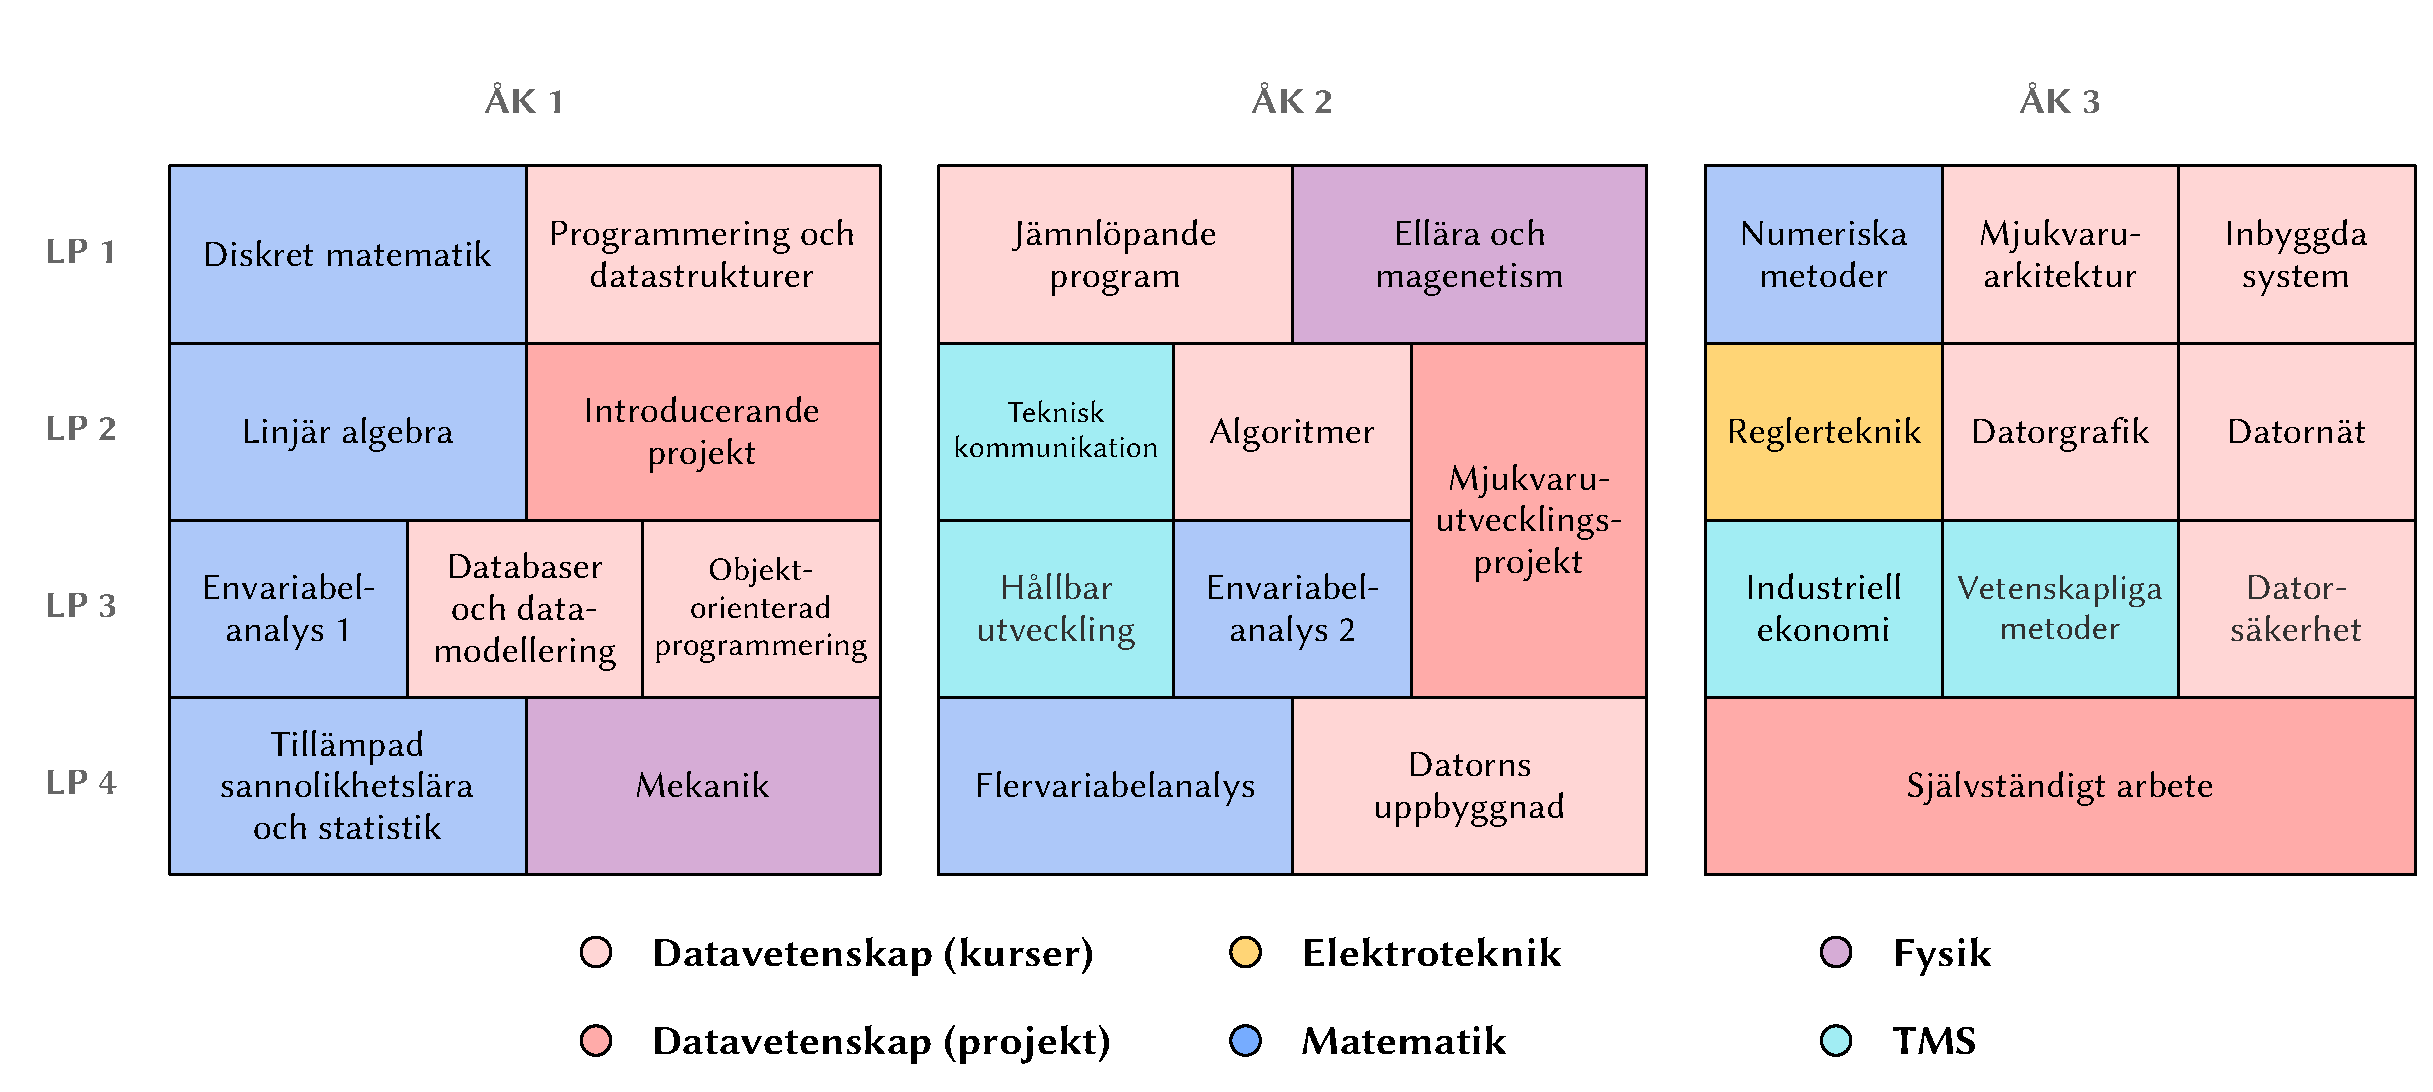
\includegraphics[width=\columnwidth]{images/bs13.eps}
\caption{Upplägg årskurs 1--3. Varje läsperiod omfattar 15 hp och kurserna omfattar 5, 7,5 eller 10 hp. Det självständiga arbetet omfattar 15 hp.\label{fig:bs13}}
\end{figure}

Årskurs 1--3 motsvarar innehållsmässigt en kandidatutbildning inom datavetenskap med särskilt fokus på yrkesmässighet och teknik, människa och samhälle. Figur~\ref{fig:bs13} beskriver innehåll och progression under årskurs 1--3. Det datavetenskapliga innehållet är upplagt enligt ACM och IEEE:s\footnote{Institute of Electrical and Electronics Engineers~(IEEE) (\url{https://www.ieee.org}), en internationell branchorganisation för ingenjörer inom elektroteknik, telekommunikation, och datateknik.} gemensamma rekommendationer för innehåll i utbildning på grundnivå (ACM CS2013)\footfullcite{cs2013}. Conceive-Design-Implement-Operate (CDIO)-konceptett\footfullcite{crawley2014rethinking} används för att säkerställa att utbildningen och dess kurser innehåller en hög nivå av ingenjörsmässighet. Innehållet i kurserna i matematik och fysik är valt för att ge en tillräcklig grund inom dessa ämnen samt stödja kurser i karaktärsämnet.

Då upplägget och kurserna bygger på ACM CS2013 påminner blockschemat om flera andra grundutbildningar inom datavetenskap vid Linnéuniversitetet. Under arbetet med det föreslagna utbildningsprogrammet har stor vikt lagts vid progression och färdighetsbyggande. Innehållet i årskurs 4 och 5 definierades först och sedan planerades årskurs 1–3 så att de bygger upp de färdigheter och kunskaper som behövs. Resterande delen av avsnittet fokuserar på de huvudsakliga progressionsspåren.

Det finns ett starkt samspel mellan datavetenskap och matematik, men detta är av erfarenhet svårt att kommunicera till studenterna. Det föreslagna programmet skapar därför tydliga kopplingar mellan kurserna i datavetenskap och matematik under årskurs 1. Under läsperiod 1 får studenterna se datastrukturer från ett datavetenskapligt perspektiv i \emph{Programmering och datastrukturer} och från ett matematiskt perspektiv i \emph{Diskret matematik}. Den senare innehåller inte någon undervisning i programmering, men kommer att ha frivilliga programmeringsuppgifter som studenterna kan göra för att utforska likheterna och för att ta sig an matematiken från ett datavetenskapligt perspektiv. I läsperiod 2 presenteras programmering i Matlab i kursen \emph{Linjär algebra} och studenterna kan direkt tillämpa färdigheter från datavetenskap. På liknande sätt tillämpas begrepp från matematiken, exempelvis funktionsbegreppet och matematisk logik, i kursen \emph{Databaser och datamodellering} i läsperiod 3. I övriga kurser i datavetenskap och matematik använder, när tillämpbart, exempel från det andra ämnet, det vill säga datavetenskapliga tillämpningar inom kurserna i matematik och matematiska problem i kurserna i datavetenskap. I kursen \emph{Numeriska metoder} i läsperiod 1, årskurs 3 studeras bland annat numeriska grafalgoritmer och Bézier-kurvor, som båda har flera tillämpningar inom datavetenskap.

Programmering är en grundläggande färdighet och utbildningen är byggd runt fyra programmeringsspråk: C, Java, Matlab och Python. En kurs kan, så länge den ges efter språket introducerats, välja att använda det av dessa som bäst lämpar sig för kursens innehåll eller låta studenterna välja fritt. Om en kurs behöver ett annat språk ingår det som lärandemål för kursen. Kursen \emph{Programmering och datastrukturer} lär ut grundläggande imperativ programmering och vissa koncept från funktionell programmering med hjälp av Python. Det föreslagna programmet börjar med ett programmeringsspråk som anses lätt att lära sig för att kunna lägga fokus på problemlösning och algoritmer. Kursen \emph{Objektorienterad programmering} bygger vidare på dessa färdigheter och lär ut objektorienterad programmering i Java medan kursen \emph{Datorns uppbyggnad} fokuserar på hårdvarunära programmering med C. Matlab ingår i kurserna i matematik och introduceras i kursen \emph{Linjär algebra}.

Vårt upplägg medför att studenterna får lära sig tre programmeringsspråk under årskurs 1. Detta upplägg har valts för att belysa att programmeringsspråket är ett verktyg och att olika språk är mera lämpliga än andra i vissa situationer. Vart och ett av språken kommer att användas i en rad kurser under utbildningen och på så sätt fördjupa studentens förståelse för och färdighet i språket.

En annan grundläggande färdighet är modellering och tänkande i modeller. Detta börjar ur ett mjukvaruutvecklingsperspektiv i kurserna \emph{Databaser och datamodellering} och \emph{Objektorienterad programmering} i årskurs 1, där studenterna får två olika perspektiv på objektorienterad modellering samt en introduktion till problemlösning på modellnivå med designmönster. Studenterna tillämpar dessa färdigheter i kursen \emph{Mjukvaruutvecklingsprojekt} i årskurs 2 och de fördjupas i kursen \emph{Mjukvaruarkitekturer} i årskurs 3.

Yrkesfärdigheter och ingenjörsmässighet undervisas genom kurser i teknik, människa och samhälle samt en serie projektkurser. Studenterna introduceras till yrkesrollen mjukvaruingenjör redan i kursen \emph{Programmering och datastrukturer}, genom de verktyg som används och enklare samarbetsformer (exempelvis parprogrammering). Detta byggs vidare i kursen \emph{Introducerande projekt}, där studenterna ges insikt i yrkesrollen genom bland annat gästföreläsningar och studiebesök. Projektarbetet sker under enkla men realistiska förhållande och täcker hela Concieve-Design-Implement-Operate-cykeln från CDIO-konceptet. Det ger på så sätt ytterligare insikt i de verktyg och arbetssätt som används och vikten av att förstå vilket problem ett mjukvarusystem skall lösa.

I årskurs 2 fångas erfarenheterna från tidigare ämnes- och projektkurser upp i \emph{Teknisk kommunikation} och \emph{ållbar utveckling}. Den första av dessa belyser rapportskrivande och muntlig presentation. Den senare belyser hållbarhet ur sociala, miljömässiga och ekonomiska perspektiv. I kursen \emph{Introducerande projekt} reflekterar studenterna över yrkesrollen mjukvaruingenjör från ett personligt perspektiv. Efter denna introduktion kan ett socialt perspektiv läggas till genom att studenterna exempelvis inom ramen för inlämningsuppgifter reflekterar över den ojämna könsfördelningen inom mjukvaruindustrin och vilken påverkan den har i stort. Kursen \emph{Mjukvaruutvecklingsprojekt} fördjupar förståelse för yrkesrollen, dels genom ytterligare gästföreläsningar eller studiebesök, men främst genom en fördjupning i de verktyg och de arbetssätt som används. Kursen består av ett realistiskt projekt där studenterna löser ett problem åt en kund genom att tillämpa en agil mjukvaruutvecklingsprocess. Kursen \emph{Industriell ekonomi} i årskurs 3 belyser ekonomi ur ett industriellt perspektiv och påvisar skillnader och likheter mellan exempelvis traditionell tillverkningsindustri och mjukvaruindustrin, såsom utvecklings- kontra tillverkningskostnad. Ekonomi beskrivs också ur ett samhällsperspektiv där exempelvis mjukvarans ökande roll diskuteras och hur det kommer att påverka samhälle och industri.

Kurserna inom teknik, människa och samhälle har utformats och placerats så att det ämne som behandlas inom en kurs kan introduceras innan kursen ges och sedan kan byggas vidare på och fördjupas. Hållbarhet lyfts fram ur olika perspektiv under kurserna i årskurs 1 på en ytlig nivå (Introduceras, enligt CDIO-terminologi) och dessa perspektiv fångas upp och fördjupas inom kursen hållbar utveckling (Undervisas). I efterföljande kurser behandlas hållbarhetsperspektiven djupare och erfarenheter och teorier används direkt (Undervisas och Används).

Årskurs 3 avslutas med två kurser som samlar upp erfarenheter och perspektiv från tidigare kurser. Den första av dessa är kursen \emph{Datorsäkerhet}, som diskuterar erfarenheter från bland annat kurserna \emph{Databaser och datamodellering} och \emph{Datornät} och belyser dem ur ett säkerhetsperspektiv. Frågeställningar såsom vilka problem som finns, hur de kan lösas, samt hur man tänker kring säkra system diskuteras. Dessa perspektiv kommer, likt perspektiv från kurserna i teknik, människa och samhälle, tas med i framtida kurser och beröras där det är tillämpligt. Den andra sammanfattande kursen är det självständiga arbetet, där studenterna tillämpar kunskaper och färdigheter från årskurs 1–3 för att formulera och lösa ett problem, samt beskriva och argumentera för lösningen. Dessa färdigheter är viktiga och det föreslagna programmet innehåller därför ett självständigt arbete om 15 hp i slutet av årskurs 3, för att sammanfatta och förbereda studenterna inför studier på avancerad nivå, där den vetenskapliga kopplingen och kraven på bland annat rapporter skärps.

\subsection{Utbildningens innehåll och progression årskurs 4--5}

\begin{figure}[tbp]
\centering
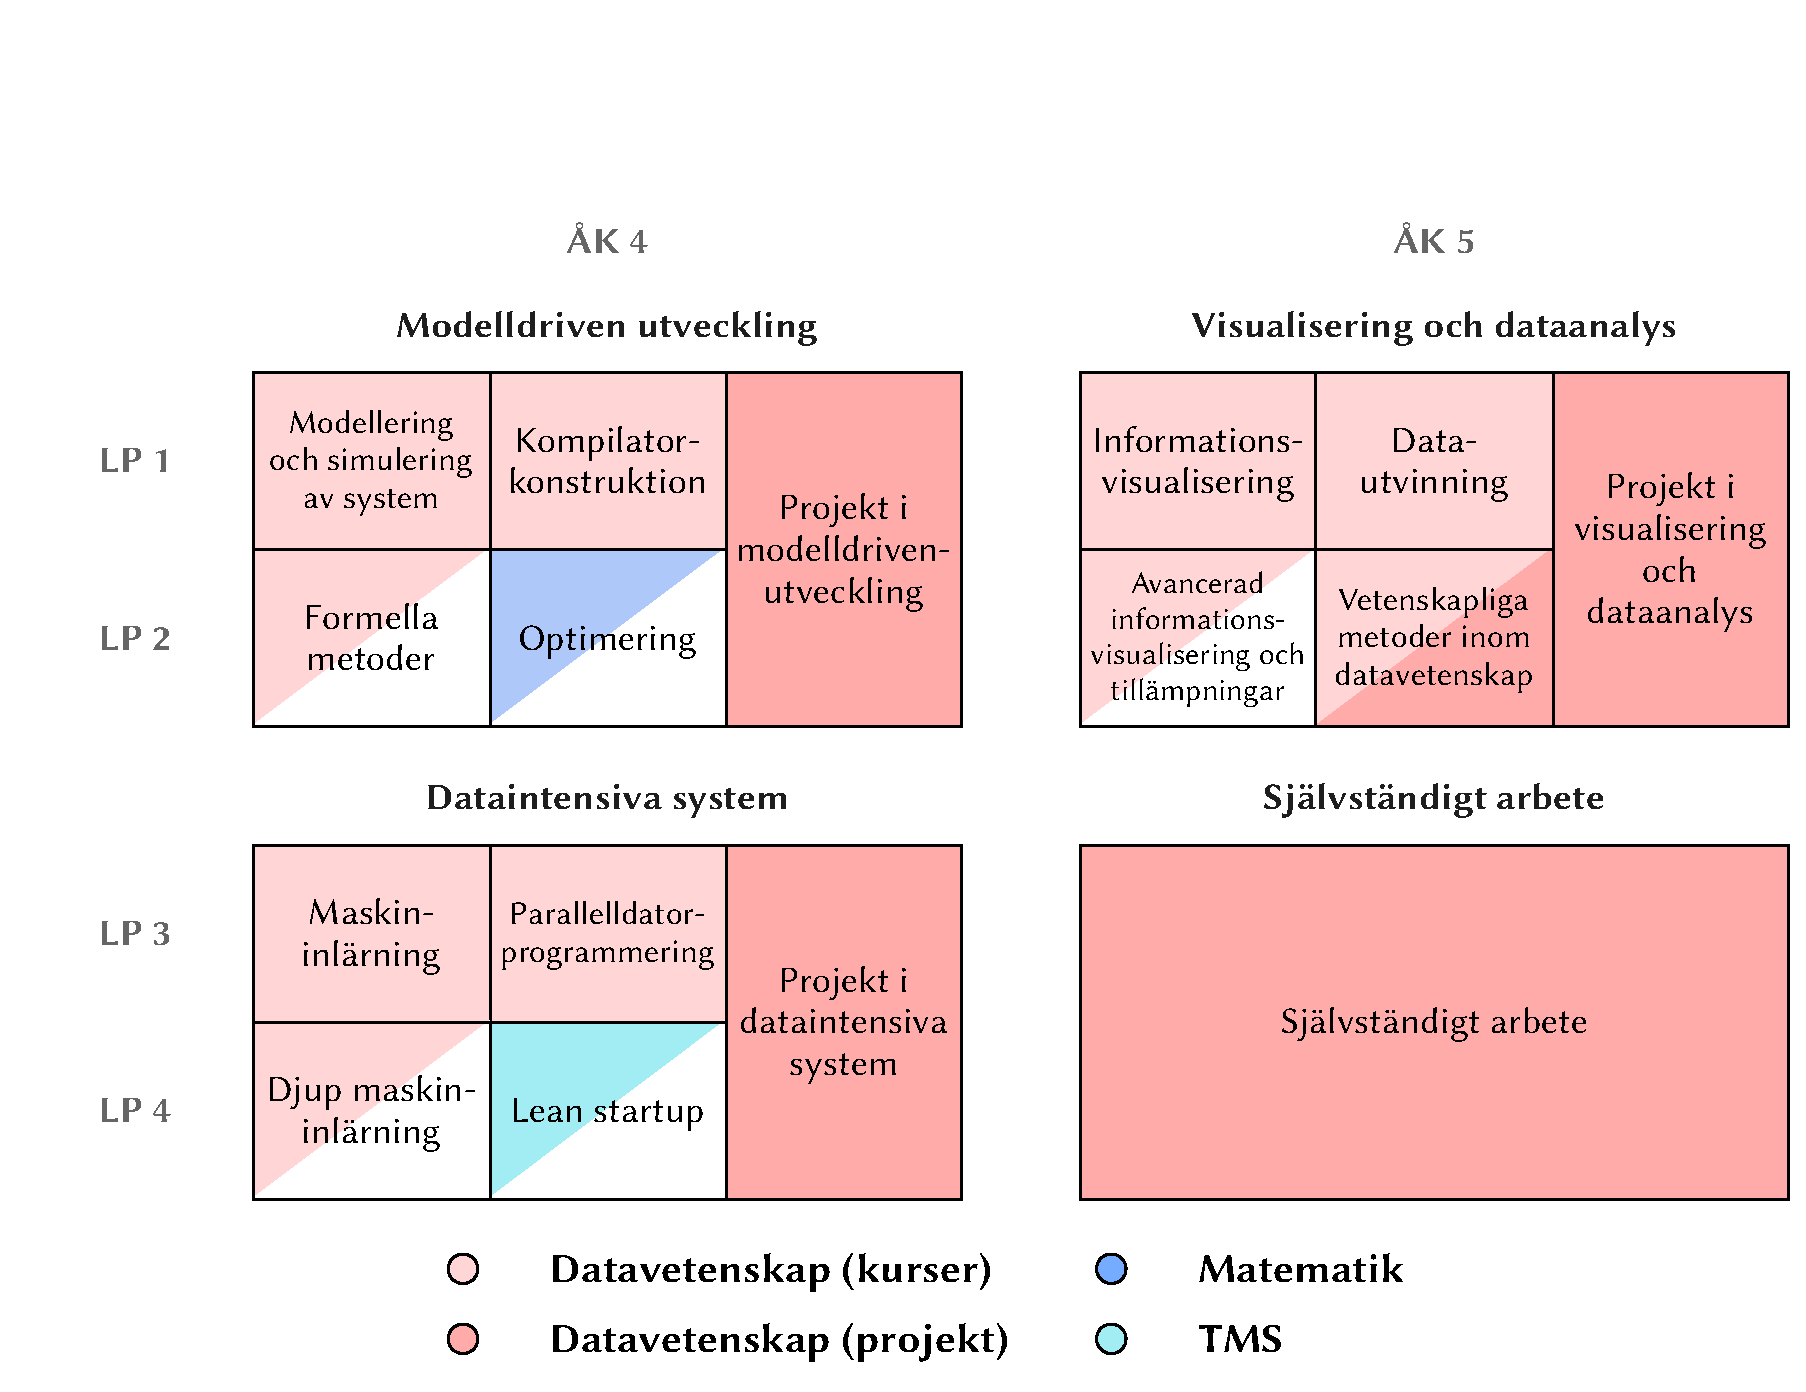
\includegraphics[width=\columnwidth]{images/bs45.eps}
\caption{Upplägg årskurs 4--5. Termin 7--9 består vardera av fyra kurser och ett projekt och termin 10 består av ett självständigt arbete.\label{fig:bs45}}
\end{figure}

Årskurs 4 och 5 ger en fördjupning i karaktärsämnen och yrkesrollen. Figur~\ref{fig:bs45} beskriver innehåll och progression under årskurs 4 och 5. Under termin 7–9 läser studenterna fyra kurser (5 hp vardera) och ett projekt (10 hp) varje termin. De fyra kurserna ger en teoretisk fördjupning och projektet, som täcker hela CDIO-cykeln, ger praktiska färdigheter och fördjupning inom yrkesrollen. Det ger även studenterna möjlighet att snabbt omsätta de mera teoretiska kunskaperna och frågeställningarna från kurserna inom exempelvis etik eller mjukvarans roll i samhället i ett praktiskt projekt. Under termin 10 genomför studenterna ett självständigt arbete som omfattar 30 hp. Termin 7–9 kommer att ha terminskoordinatorer som ansvarar för att skapa ett sammanhang mellan kurser och projekt. Terminskoordinatorn kommer att vara en senior forskare från aktuellt fördjupningsområde som tillsammans med en expert på projekt och projektmetodik ansvarar för terminens projekt.

Varje termin har ett fördjupningsområde inom det övergripande temat modellens roll i mjukvaruutveckling och ger något eller några perspektiv på hur modeller används. De tre fördjupningsområdena är starkt kopplade till forskning inom datavetenskap. Den forskargrupp som står närmast ett område ansvarar för projektet och en majoritet av kurserna.

Termin 7, \emph{Modellbaserad utveckling}, fokuserar på hur modeller kan användas för att utveckla eller testa egenskaper hos system. Terminen börjar med kurserna \emph{Modellering och simulering av system} och \emph{Kompilatorkonstruktion}. Den första av dessa två diskuterar hur man kan modellera och simulera ett system för att exempelvis testa egenskaper hos systemet innan implementationen i något programspråk påbörjas. Den senare kursen fokuserar på datorspråk och översättningar mellan dessa och belyser hur modellbeskrivningsspråk kan översättas till programspråkskod eller exekverbar kod. Under projektkursen kommer studenterna att tillämpa modellbaserad utveckling för att lösa ett öppet problem i en realistisk miljö, medan kurserna belyser den teori och de algoritmer som exempelvis de verktyg som används bygger på. Studenterna får i kurserna implementera enklare versioner av verktygen och i projektet använda verktyg som används i yrkeslivet. Terminen avslutas med kurserna \emph{Formella metoder} och \emph{Optimering} som fokuserar på hur egenskaper hos en modell kan formellt verifieras samt hur modeller kan optimeras.

Termin 8, \emph{Dataintensiva system}, fokuserar på hur modeller kan utvinnas och läras ur data. Terminen inleds med kurserna \emph{Maskininlärning} och \emph{Parallelldatorprogrammering}. I den första introduceras algoritmer för maskininlärning för att analysera och identifiera information i stora datamängder. I den senare ges en insikt i hur stora beräkningar kan utföras mer effektivt genom parallellbearbetning och vilka typer av utmaningar detta kan medföra. Projektkursen ger studenterna praktiska erfarenheter koppade till modellering och tillämpning av algoritmer för maskininlärning. Kursen \emph{Djup maskininlärning} är en fortsättningskurs som belyser aspekter som kräver viss erfarenhet såsom hur man utvärderar resultat, hur mycket data som behövs, eller när olika algoritmer är tillämpliga, vilket studenterna får i det pågående projektet.

Termin 9, \emph{Visualisering och dataanalys} fokuserar på visualisering och hur modeller kan kommuniceras till människor för vidare, fördjupad, analys. De två första kurserna \emph{Informationsvisualisering} och \emph{Datautvinning} ger grunderna i hur man visualiserar information samt hur man utvinner data ur ostrukturerade källor. Kurserna ger tillsammans den grundläggande förståelse som behövs i projektet som handlar om analys med stöd av visualiseringar, ett arbetssätt där människan med hjälp av avancerade flexibla visualiseringar försöker förstå komplexa modeller och den information som dessa innehåller. Kursen \emph{Avancerad informationsvisualisering} och tillämpningar bygger vidare på de inledande kurserna och på projektkursen och belyser hur visualisering tillämpas inom exempelvis bioinformation och geografi.

De tre projekten i termin 7–-9 ger förutom en möjlighet att tillämpa kunskaper från de olika fördjupningsområdena, även en progression i yrkesrollen och att arbeta i projekt. Det första av de tre projekten ger studenterna möjlighet att mera självständigt pröva några av de olika metoder och aktiviteter inom agila utvecklingsprocesser som introducerades i kursen \emph{Mjukvaruutvecklingsprojekt} i årskurs 2. I det andra projektet läggs fokus på att göra ett utvecklingsteam så effektivt som möjligt, genom att införa så kallade Lean agile-metoder. Här låter man studenterna arbeta under former som påminner om en startup, där tid och resurser är begränsade. I den tredje projektkursen skall studenterna självständigt genomföra ett agilt projekt.

Termin 10 består av ett självständigt arbete som avslutar och sammanfattar utbildningen. För att förbereda inför detta ges en fördjupning i \emph{Vetenskapliga metoder inom datavetenskap} i termin 9. Det är en seminariekurs där studenter läser, presenterar och diskuterar/opponerar på vetenskapliga artiklar, med fokus på vetenskapliga frågeställningar och metod. Studenterna väljer, i samråd med forskare från de olika fördjupningsområdena, lämpliga artiklar att läsa. En stor del av kursens examination är att ta fram ett planeringsdokument med frågeställningar och metod för det självständiga arbetet.

\subsection{Utbildningens vetenskapliga grund och forskningsanknytning}

 CDIO-konceptet används för att säkra att det föreslagna utbildningsprogrammet uppnår en hög nivå av ingenjörsmässighet. Det kan vara svårt att tydligt skilja vetenskap och ingenjörskonst, särskilt inom tillämpade vetenskaper. Det finns tillämpad forskning och grundläggande ingenjörskonst. Det är inte självklart att den ena står närmare forskning och vetenskap än den andra. De två likställs därför under programmets inledning och tidiga kurser fokuserar på att ta fram tekniska lösningar till komplexa problem och verifiera dessa lösningar samtidigt som ett helhetsperspektiv krävs. På liknande sätt övar bland annat kurserna \emph{Databaser och datamodellering} och \emph{Objektorienterad programmering} studenterna i att värdera och prioritera olika lösningar till ett problem, samt argumentera för dessa. Kursen \emph{Tillämpad sannolikhetslära och statistik} i slutet av årskurs 1 täcker hypoteser, experiment och hypotesprövning, som sedan kommer att tillämpas i kommande kurser.

I årskurs 3 ger kursen \emph{Vetenskapliga metoder} en introduktion till metodik och hur man genomför en vetenskaplig studie. Kursen belyser kopplingen till ingenjörsmässighet samt samspelet mellan vetenskap och ingenjörskonst. I det självständiga arbetet i slutet av årskurs 3 ska studenterna självständigt formulera ett problem i samråd med en handledare och en lösning till detta, samt påvisa att det är en lösning. De skall använda ingenjörsmässiga och/eller vetenskapliga metoder för det. Innan studenterna får lägga fram sitt självständiga arbete skall de ha auskulterat på tre andra framläggningar, på minst samma nivå. För att förbereda dem inför det egna självständiga arbetet uppmanas studenterna från och med termin 4 att börja auskultera på andra arbeten, främst på kandidatnivå. Det kan också göras vid arbeten på högre nivå till exempel masters, licentiat eller doktor. Studenterna skall även auskultera på tre arbeten på mastersnivå eller högre inför det självständiga arbetet i termin 10 och de kommer att uppmuntras göra detta från och med termin 6.

I årskurs 4 och 5 kopplas i princip samtliga kurser till den forskning som bedrivs inom Institutionen för datavetenskap och medieteknik såsom dataintensiv mjukvaruteknik och informationsvisualisering. Kurserna och projekten kommer under dessa årskurser att ha en väldigt tydlig anknytning till aktuell forskning och forskningsresultat. Många av de metoder och verktyg, samt den plattform som används för laborationer, kommer direkt från eller används inom forskningen vid institutionen.

Under årskurs 4 och 5 kommer en stor del av kurslitteraturen att bestå av vetenskapliga artiklar, men redan under årskurs 1 kommer vissa kurser att använda vetenskapliga artiklar som komplement till kurslitteraturen. Ett exempel på en sådan artikel är E.F. Codds ``A Relational Model of Data for Large Shared Data Banks'' från 1970 som introducerar relationsmodellen som fortfarande är den dominerande modellen för databaser. Syftet med artiklarna som används på kurserna under årskurs 1 är främst att öva studenterna på att söka efter och läsa vetenskapliga artiklar, samt påminna om att stora idéer ofta börjar som vetenskapliga resultat i artiklar. Under årskurs 2 och 3 ökar antalet kurser som använder vetenskapliga artiklar som komplement och syftet med artiklarna breddas till att också vara ett innehållsmässigt komplement till kurslitteraturen.

I kursen \emph{Teknisk kommunikation} i årskurs 2 undervisas i hur man söker efter information och artiklar, hur man läser en artikel, samt hur man analyserar och bedömer en artikels innehåll. I kursen \emph{Introducerade projekt} i årskurs 1 skall studenterna söka efter information för att lösa problem, men detta rör sig främst om teknisk information som snabbt kan utvärderas. Efter undervisning i hur man söker och analyserar artiklar kommer kurserna att ställa större krav på att självständigt söka information och ta ställning till denna. Denna färdighet byggs vidare på i kursen \emph{Vetenskapliga metoder}, där studenterna undervisas i att värdera metoder och hur dessa påverkar vilka frågor som kan besvaras samt hur tillförlitligt och generaliserbart resultatet är. Det självständiga arbetet i slutet av årskurs 3 är den första kursen där studenterna själva ska välja all litteratur (i samråd med handledare). I årskurs 4 och 5 skall studenterna självständigt söka efter och välja kompletterande litteratur i de flesta av kurserna, i synnerhet projektkurserna.

Under årskurs 1–3 kommer den programansvarige att ha det operativa ansvaret för att det finns forskningsanknytning och ett forskande perspektiv i utbildningen. Under termin 7–9 flyttas detta ansvar till terminskoordinatorerna, som är experter inom det området som fördjupningen berör. Under termin 10 delas det operativa ansvaret mellan handledarna och examinatorerna för de självständiga arbetena.

\section{Motivering för ansökan om examensrättigheter}

Linnéuniversitetet söker rättigheter att examinera civilingenjörer i mjukvaruteknik av tre skäl. Nedan följer bakgrund till, analys av och motivering för dessa.

\begin{itemize}
	\item Industrin, både i regionen och nationellt, har ett stort behov av att rekrytera kvalificerad arbetskraft och efterfrågar särskilt civilingenjörer inom data och informationsteknik.
	\item Linnéuniversitetet har en stark tradition av yrkesutbildning och strävar mot ett brett erbjudande med hög kvalitet. Universitetet har därför arbetat strategiskt för att utöka sitt erbjudande med en examensrättighet för civilingenjörer.
	\item Fakulteten för teknik vill erbjuda en spetsutbildning med högre grad av ingenjörsmässighet och yrkeslivskoppling inom datavetenskap.
\end{itemize}

Den regionala industrin har under flera år efterlyst en regional civilingenjörsutbildning inom data och informationsteknik då de upplever att det är väldigt svårt att rekrytera personer med civilingenjörsutbildning till regionen. Flera anger att de har slutat att försöka och överväger alternativa lösningar som att omlokalisera delar av eller hela sin verksamhet. Många företag och kommunerna i regionen anser att den föreslagna civilingenjörsutbildningen är avgörande för en fortsatt tillväxt i regionen och, i ett längre perspektiv, vissa verksamheters långsiktiga överlevnad. Till ansökan bifogas stödbrev och avsiktsförklaringar från industri och organisationer i regionen (Växjö och Kalmar) i appendix~\ref{app:stodbrev}. Stödbrev för att belysa deras behov och intresse av en civilingenjörsutbildning i regionen.

Att förse regionen och landet med kompetent arbetskraft är en av universitetets främsta uppgifter och därför framhålls detta som den främsta anledningen till att Linnéuniversitetet söker examensrättigheter. Den föreslagna utbildningen är dock inte avsedd som en regional utbildning utan är byggd för att motsvara det nationella behov som anges i avsnitt~\ref{sec:analysindbehov} och studenter kommer efter examen att kunna söka sig regionalt, nationellt och internationellt. Erfarenhet från befintliga längre yrkesutbildningar visar dock att några studenter antingen söker sig till utbildningen för att de inte vill lämna regionen eller under sin studietid rotar sig i regionen och således stannar kvar efter examen. Det stora inslaget av projekt som utförs tillsammans med näringslivet kommer troligtvis att leda till att studenter rekryteras av företag i regionen. Det här resonemanget stöds av en rapport från Teknikföretagen\footfullcite{teknikforetagen} som menar att det bästa sättet att rekytera utanför storstadsregionerna är att samarbeta med universitet och högskolor i regionen (se avsnitt~\ref{sec:analysindbehov}).

Nästa skäl till ansökan av examensrättigheter är att Linnéuniversitetet har en lång tradition av yrkesutbildningar, exempelvis högskoleingenjör och lärare. Samtidigt är universitetet idag ett av få svenska lärosäten som inte har rättigheter att examinera civilingenjörer. Då detta är en efterfrågad examen av både industri och studenter är det av strategisk vikt att erhålla rättigheter att erbjuda denna examen, för att säkerställa möjligheter att rekrytera studenter inom teknikområden i framtiden. Linnéuniversitetet tappar redan studenter som vill läsa vidare mot en civilingenjörsexamen efter sin högskoleingenjörsexamen, då en masterexamen inte uppfattas ha samma värde som en civilingenjörsexamen. Baserat på det söktryck och intresse som finns för de befintliga civilingenjörsutbildningarna inom data och informationsteknik (se avsnitt~\ref{sec:analysbefintnat}) anser Linnéuniversitetet att det finns utrymme för flera utbildningar.

De två skäl som anges ovan är viktiga, men de kräver att en utbildning av hög kvalitet kan erbjudas. Så, det sista skälet till att Linnéuniversitetet söker rättigheter är att det kan erbjuda en högkvalitativ utbildning som tillför något utöver det som erbjuds av de befintliga civilingenjörsutbildningarna inom data och informationsteknik. Det utbildningsprogram som föreslås i ansökan började som ett initiativ att göra det befintliga mastersprogrammet i mjukvaruteknik mera anpassat mot yrkeslivets behov, genom att bland annat öka inslag av projekt och ingenjörsmässighet. Samtidigt har programmets starka koppling mot forskning bibehållits. Arbetet resulterade bland annat i upplägget med tre korta fördjupningar med både en teoretisk och en praktisk fördjupning. Arbetet med att förändra mastersprogrammet finansierades av KK-stiftelsen\footnote{``Nyutveckling av masterprogrammet i datavetenskap'', KK-stiftelsen Dnr: 20150316} och skedde i samarbete med näringslivet i regionen (Kronoberg, Kalmar och Blekinge), exempelvis Combitech och IKEA. När årskurs 4 och 5 var klara skapades innehållet i årskurs 1–3 för att på bästa möjliga sätt förbereda studenterna. Det finns en tydlig progression genom programmet, där studenternas kunskaper, färdigheter och perspektiv inom och på datavetenskap, matematik, ingenjörsmässighet och vetenskaplighet utvecklas. Den stora andelen projektkurser kommer att förbereda studenterna för yrkeslivet, i linje med vad IT\&Telekombolagen\footfullcite{ittelekom} föreslår för att förbättra arbetslivsförberedelserna inom utbildningen.

\section{Analys av behov i ett regionalt och nationellt perspektiv}\label{sec:analysindbehov}

Teknikföretagen, IT\&Telekomföretagen och Swedsoft\footfullcite{swedsoft} har i slutet av 2017 och under inledningen av 2018 publicerat rapporter som kartlägger kompetensbehov inom data och informationsteknik i svensk industri. Man är överens om att mjukvara får en allt större roll i samhället och ekonomin. Dessutom finns det ett stort rekryteringsbehov av ingenjörer med mjukvaruspecialisering. Samtidigt visar rapporterna på att detta är en av de mest bekymmersamma kompetenserna att rekrytera; IT\&Telekombolagen benämner kompetensbristen inom IT-sektorn ``en av vår tids största utmaningar''.

Enligt Statistiska centralbyråns arbetskraftsbarometer för 2017 bedömer 8 av 10 arbetsgivare att de kommer att öka antalet anställda med civilingenjörsutbildning inom datateknik till 2020\footfullcite{barometern17}. Samtidigt bedömer mer än 60~\% av tillfrågade arbetsgivare att det finns en brist på nyutexaminerade och mer än 80~\% anser att det finns en brist på yrkeserfarna. I samma undersökning rapporteras en ännu större brist av programmerare och systemvetare; här anser nästan 80~\% av arbetsgivarna att det råder brist. Så även om civilingenjörsprognosen innefattar elektronik och automation är det rimligt att använda den för att dra slutsatser för datateknik och datavetenskap.

Swedsofts rapport menar att heterogeniteten i gruppen mjukvaruutvecklare medför att kompentenserna som krävs varierar från företag till företag. Den absolut viktigaste kompetensen är generell programmeringskompetens följd av specifik systemnära programmering. Viktiga kompletterande kompetenser som söks är bland annat system- och systemarkitekturkompetens och matematisk kompetens, medan kunskap inom ekonomi och affärsverksamhet anses minst viktigt av de som undersöks. Bland de viktiga kompletterande förmågor som söks står tre ut: logiskt analytisk förmåga (cirka 90~\% anser denna avgörande), kreativ och innovativ (cirka 80~\%), samt självledarskap och självkännedom (cirka 80~\%). Förmågor såsom ledarskap anses mindre avgörande (cirka 45~\%). Djupintervjuer med deltagare belyser särskilt behovet av samarbete mellan mjukvaruutvecklare och personer med andra kompetenser, exempelvis nämns fysiker och mekaniker som viktiga för automation och robotar.

Precis som i rapporten från Swedsoft menar IT\&Telekombolagen att generell programmeringskompetens är viktigare än specifik kunskap i ett särskilt språk. De efterlyser också bättre arbetslivsförberedelser från högskoleutbildningar genom fortlöpande färdighetsträning och arbetslivskontakter under utbildningstiden. De föreslår specifikt att det skall finnas två obligatoriska kursmoment i aktivt samarbete med tänkbara framtida arbetsgivare. De menar vidare att en sådan ansats även kan hjälpa till att öka kompetensen hos de arbetsgivare som medverkar i dessa moment, så att det blir en dubbelriktad satsning.

\section{Analys av befintligt regionalt och nationellt utbildningsutbud}\label{sec:analysbefintnat}

Hösten 2017 erbjöds det totalt 19 civilingenjörsutbildningar inom data och informationsvetenskap vid 13 lärosäten. En stor del av dessa har generella benämningar såsom Datateknik, Informationsteknik och Mjukvaruteknik. Innehållet i de flesta av programmen kan beskrivas som en kombination av, i ACM:s nomenklatur, Computer Science, Software Engineering och Computer Engineering. Majoriteten av programmen bedöms ha ett huvudsakligt fokus på datavetenskap (Computer Science). Programmen i Datorsäkerhet, Spel- och programvaruteknik och Robotik har mera specifika namn och i stor utsträckning även specifikt innehåll.

Den föreslagna utbildningen i mjukvaruteknik är en kombination av datavetenskap och mjukvaruteknik. Baserat på en analys av utbildningsplaner ligger den föreslagna utbildningen närmast de program som benämns Informationsteknik eller Mjukvaruteknik vid Linköping tekniska högskola, Chalmers tekniska högskola och Kungliga tekniska högskolan. Den föreslagna utbildningen skiljer sig dock från dessa på några punkter, bland annat det stora inslaget av projekt och de tre obligatoriska fördjupningsområdena. Programmet i Spel- och programvaruteknik vid Blekinge Tekniska Högskola har ett stort inslag av projekt och programvaruutveckling, men skiljer sig samtidigt då det har en fokus på datorspelsteknik.

Söktrycket för civilingenjörsutbildningar inom området är högt. Enligt UKÄ:s sök- och antagningsstatistik från 2016 och 2017 finns det fler sökande än platser. De olika programmen hade 2017 totalt nästan 14 000 sökande och nästan 2 400 förstahandssökande. De existerande program som mest liknar den föreslagna utbildningen hade totalt cirka 2 200 sökande, 640 förstahandssökande och 530 antagna.

Antalet sökande varierar stort mellan etablerade civilingenjörsutbildningar vid exempelvis Chalmers tekniska högskola och Kungliga tekniska högskolan och de nyare vid exempelvis Karlstads universitet och Örebro universitet. Det är dock endast en utbildning som 2017 inte hade några reserver, vilket tyder på att även de nyare utbildningarna fyller sina platser. Tidigare statistik visar dock på att det har tagit tid för de nyare utbildningarna att nå upp till dessa sök- och antagningstal.


\section{Analys av befintliga utbildningar inom data och informationsteknik vid Linnéuniversitetet}\label{sec:analysbefintlnu}

Linnéuniversitetet erbjuder ett högskoleexamensprogram, tre kandidatprogram, två högskoleingenjörsprogram, ett magisterprogram och ett mastersprogram inom datavetenskap och datateknik. Se tabell~\ref{tab:dvprogram} för en översikt. Utöver dessa erbjuds även utbildningar inom medieteknik och informatik på grund och avancerad nivå. De senare skiljer sig dock avsevärt från den föreslagna utbildningen och diskuteras därför inte.

\begin{table}
\centering
\caption{Utbildningsprogram inom datavetenskap och datateknik vid Linnéuniversitetet. Antagna anger det antal studenter som antogs inför läsåret 2017/2018.\label{tab:dvprogram}}
%\resizebox{\columnwidth}{!}{%
\begin{threeparttable}
\begin{tabular}{p{5cm}lrr}
\toprule
\textbf{\textsf{Namn}} & \textbf{\textsf{Examen}} & \textbf{\textsf{Hp}} & \textbf{\textsf{Antagna}}\tabularnewline
\midrule
Webbprogrammerare & Högskoleexamen & 120 & 125\tabularnewline
Datateknik & Högskoleingenjörsexamen & 180 & 39\tabularnewline
Mjukvaruteknik\tnote{1} & Högskoleingenjörsexamen & & \tabularnewline
Programvaruteknik & Kandidatexamen & 180 & 93\tabularnewline
Nätverkssäkerhet & Kandidatexamen & 180 & 64\tabularnewline
Utveckling och drift av mjukvarusystem & Kandidatexamen & 180 & 130\tabularnewline
Programvaruteknik & Magisterexamen & 60 & 24\tabularnewline
Programvaruteknik & Masterexamen & 120 & 23\tabularnewline
\bottomrule
\end{tabular}
\begin{tablenotes}
\item[1] Från och med läsåret 2018/2019.
\end{tablenotes}\end{threeparttable}
\end{table}

De befintliga utbildningarna på grundnivå täcker olika delar av datavetenskap och datateknik. Högskoleingenjörsprogrammet i datateknik täcker områdena mellan mjukvara och hårdvara och fokuserar i huvudsak på inbyggda system. Kandidatprogrammet i programvaruteknik är en traditionell datavetenskaplig utbildning med fokus på mjukvaruutveckling, medan kandidatprogrammen i \emph{Nätverkssäkerhet} och \emph{Utveckling och drift av mjukvarusystem} har en datavetenskaplig kärna men ett starkt fokus på tillämpningsområden. Nätverkssäkerhet fokuserar på datorsäkerhet med avseende på både mjukvara och datornät och innehåller bland annat kurser i kryptering och administration av nätverk. Utveckling och drift av mjukvarusystem fokuserar på området mellan mjukvaruutveckling och systemdrift, så kallade Development Operations (DevOps) och innehåller bland annat kurser i systemadministration, kontinuerlig leverans av mjukvara och konfigurationshantering. Högskoleprogrammet i webbprogrammering är en yrkesförberedande utbildning som fokuserar på utveckling av mjukvara för webben exempelvis webbplatser och backend-system.

I ansökningsomgången 2017 sökte totalt cirka 3 400 studenter, varav 587 förhandssökande, till våra fem utbildningar på grundnivå. De två mest populära programmen, \emph{Webbprogrammerare} och \emph{Utveckling och drift av mjukvarusystem} stod för över 70~\% av det totala söktrycket. Av de sökande antogs 428 och 313 registrerades.

Det föreslagna civilingenjörsprogrammet är innehållsmässigt mest likt \emph{Högskoleingenjörsprogrammet i datateknik} och \emph{Kandidatprogrammet i programvaruteknik}. Dessa hade totalt 518 sökande (99 i första hand) i ansökningsomgången 2017, varav 132 antogs och 98 registrerades.

Utbildningsutbudet inom datavetenskap vid Linnéuniversitetet ses kontinuerligt över och förändras efter behov. Inför läsåret 2018/2019 kommer exempelvis ett nytt högskoleingenjörsprogram i mjukvaruteknik startas i Kalmar och inför läsåret 2019/2020 kommer de befintliga utbildningarna på avancerad nivå förändras så att de tydligare följer det upplägg som föreslås för civilingenjörsprogrammet. Det möjliggör samläsning och medför ett större utbud av valbara kurser för den föreslagna utbildningen. Om rättigheter att examinera civilingenjörer erhålls kommer hänsyn att tas till detta vid framtida utbildningsöversyn.

\chapter{Lärarkompetens och lärarkapacitet\label{ch:personal}}

\begin{tcbdoublebox}
\emph{Avsnittet täcker aspekten Personal i den föreslagna ansökningsmallen. Här anges vilken kompetens som finns inom de institutioner som är inblandade i genomförandet av den föreslagna utbildningen samt en analys om varför denna anses vara tillräcklig. Avsnittet innehåller även en diskussion kring lärarnas utrymme för och tillgång till kompetensutveckling.}
\end{tcbdoublebox}

\section{Lärarresurser för undervisning, handledning och examination}

Institutionen för datavetenskap och medieteknik kommer att få det direkta ansvaret för att genomföra det föreslagna civilingenjörsprogrammet. Institutionerna för matematik, fysik och elektroteknik samt maskinteknik är delaktiga i det föreslagna civilingenjörsprogrammet och ansvarar för kurser eller moment inom kurser. Kurserna i teknik, människa och samhälle hämtas från de institutioner som är bäst lämpade att tillsammans med lärare från Institutionen från datavetenskap och medieteknik undervisa inom ämnet, exempelvis Institutionen för byggd miljö och energiteknik när det gäller miljöaspekterna inom hållbar utveckling. En preliminär lista över kursansvariga och examinatorer anges i appendix~\ref{app:examinatorer} och en lärartabell bifogas ansökan som separat dokument.

Den formella kompetensen har både den bredd och det djup som behövs för att säkerställa att kompetenta lärarresurser finns att tillgå i alla utbildningens kurser för undervisning, handledning och examination. Nedan följer en översiktlig beskrivning över de institutioner som är involverade i utbildningen:

\begin{itemize}
	\item Institutionen för datavetenskap och medieteknik har 5 professorer, 5 docenter, 16 lektorer, 17 adjunkter varav 3 i forskarutbildning, 2 forskarassistenter, 2 postdoktorer och 17 doktorander.
	\item  Institutionen för matematik har 6 professorer samt 1 gästprofessor, 6 docenter, 5 lektorer, 14 adjunkter varav 3 i forskarutbildning, 1 postdoktor och 6 doktorander.
	\item  Institutionen för maskinteknik har 4 professorer, 2 docenter, 3 lektorer, 4 universitetsadjunkter och 4 doktorander.
	\item Institutionen för maskinteknik har 4 professorer, 2 docenter, 3 lektorer, 4 universitetsadjunkter och 4 doktorander.
\end{itemize}

Enligt de lokala reglerna för examinationer vid Linnéuniversitetet\footfullcite{lr_examination} skall examinator för kurser på grundnivå minst vara disputerad inom relevant ämne (motsvarande lektor i våra tabeller) och för kurser på avancerad nivå minst vara docent inom relevant ämne. Vad det gäller kompetens att undervisa på eller examinera en kurs används även följande principer: den som undervisar på kurs på grundnivå skall ha tillräcklig ämneskunskap och pedagogisk färdighet och den som undervisar kurs på avancerad nivå skall dessutom vara aktiv forskare inom ämnet för kursen eller ett närliggande ämne. För att skapa forskningskoppling och ett forskande arbetssätt på kurser på grundnivå väljs lärare som antingen är forskningsaktiva i ämnet eller ett närliggande ämne i så stor utsträckning som möjligt även för dessa kurser.

Enligt Högskoleförordningen måste man visa pedagogisk skicklighet för att vara behörig att anställas som lektor eller professor, så samtliga lektorer och professorer har bedömts ha tillräcklig pedagogisk färdighet. Appendix~\ref{app:kompetens} anger vilken pedagogisk utbildning samtliga lärare som anges i appendix~\ref{app:examinatorer} har, samt om de har minst fem års erfarenhet av att undervisa inom högre utbildning. I de flesta fall är den utbildning som anges den så kallade behörighetsgivande högskolepedagogiska utbildningen som erbjuds svenska lärosäten; i de fall där utbildningen skett utomlands anges omfattningen på utbildningen i dagar eller veckor. Observera att kortare utbildningar och seminarieserier, exempelvis utbildning inom CDIO eller i kursplansskrivande, inte ger högskolepoäng och därför inte syns i sammanställningen. Många av lärarna har en bred erfarenhet från undervisning inom professionsutbildning på olika nivåer vid lärosäten i flera länder och därför presenteras även undervisningserfarenhet (i år). En lärare som har minst fem års erfarenhet av undervisning till cirka 50~\% av heltid anses vara tillräckligt, så därför anges bara ``mer än'' om en lärare har mer än fem års erfarenhet. Kompetensen hos medarbetarna har både den nödvändiga bredden och djupet för att möta kraven från en utbildning på civilingenjörsnivå.

För att uppskatta de resurser som krävs används en modell som bygger på genomsnittlig lärarresurs per högskolepoäng. Varje högskolepoäng uppskattas kräva 40 lärartimmar. Det exakta behovet varierar naturligtvis från kurs till kurs, men baserat på erfarenhet från befintliga ingenjörsprogram är detta en rimlig genomsnittlig uppskattning. Enligt denna uppskattning kräver programmet i sin helhet 12 000 lärartimmar. Observera att denna beräkning innehåller de valbara kurserna i termin 7–9 och inte tar hänsyn till eventuell samläsning. Dessa 12 000 lärartimmar fördelar sig över de olika kurserna och de ansvariga institutionerna och grupperingarna (Teknik, människa och samhälle) enligt tabell~\ref{tab:larh}. 

\begin{table}[tbh]
\caption{Fördelning av lärartimmar mellan de olika ingående institutionerna.\label{tab:larh}}
\centering
\resizebox{\columnwidth}{!}{%
\begin{tabular}{lrrr}
\toprule
\textsf{\textbf{Institution/område}} & \textsf{\textbf{Högskolepoäng}} & \textsf{\textbf{Timmar}} & \textsf{\textbf{Andel}} \tabularnewline
\midrule
Datavetenskap och medieteknik & 205~hp & 8~200~h & 68~\%\tabularnewline
Matematik & 50~hp & 2~000~h & 17~\%\tabularnewline
Fysik och elektroteknik tillsammans med maskinteknik & 20~hp & 800~h & 7~\% \tabularnewline
Teknik, människa och samhälle & 25~hp & 1~000~h & 8~\%\tabularnewline
\bottomrule
\end{tabular}}
\end{table}

En tillsvidareanställd har normalt en årsarbetstid om 1 700 timmar. Detta medför att det behövs en lärarresurs som motsvarar fem heltidsanställda vid Institutionen för datavetenskap och medieteknik för att täcka kurserna i datavetenskap. Motsvarande siffror för övriga institutioner är en heltid för Institutionen för matematik och en halvtid för Institutionen för fysik och elektroteknik samt Institutionen för maskinteknik och avslutningsvis en halvtid för kurserna inom teknik, människa och samhälle.

Professorer, docenter och lektorer kommer bära huvudansvaret för kurserna i den föreslagna civilingenjörsutbildningen och även ansvara för merparten av undervisning och examination. I utbildningen kommer dessutom adjunkter och assistenter att vara verksamma, företrädelsevis med handledning vid exempelvis laborationer och övningar, men adjunkter kommer även ta ett visst ansvar för andra undervisningsaktiviteter såsom föreläsningar på vissa grundkurser. En rimlig uppskattning, något i överkant, av fördelningen är 70/30, det vill säga att professorer och lektorer kommer ansvara för 70~\% av aktiviteter kopplat till undervisning. Med det som utgångspunkt motsvarar den seniora lärarresursen på Institutionen för datavetenskap och medieteknik 3,5 heltider för professorer och lektorer. Resterande 1,5 heltider utförs av adjunkter och assistenter.

\section{Kompetensförsörjning}

Kompetensförsörjning avser säkerställa att rätt kompetens finns för att nå de berörda verksamheternas mål både på kort och på lång sikt. Universitetet har utarbetat ett universitetsövergripande instrument, kompetensförsörjningsplanen, vilken syftar till att ge en översikt av befintlig kompetens och tydliggöra kommande kompetensbehov. Befintligt och kommande behov beskriver ett möjligt kompetensgap som används för att strategiskt planera kompetensutvecklingsbehov av befintlig personal och rekryteringar. Planerna används även för att identifiera områden där viss kompetens inte längre behövs och därmed kan avvecklas. Arbetet med kompetensförsörjning har sin grund i Linnéuniversitetets styrdokument, främst dess strategidokument, men även i beslutade policys, planer och program. Även omvärlden påverkar, exempelvis demografi, politiska beslut och konjunkturen på arbetsmarknaden. Institutionernas personalkonsulter deltar som resurs i arbetsprocesser som rör kompetensförsörjning.

Institutionen för datavetenskap och medieteknik arbetar systematiskt och rutinmässigt med kompetensförsörjningsplaner för att identifiera kortsiktiga och mer långsiktiga behov kopplade till både utbildning och forskning, både på kollegial och individuell nivå. Institutionens prefekt, ämnesansvariga och studierektor analyserar kontinuerligt behov på kort och lång sikt och dokumenterar detta i kompetensförsörjningsplanerna. Kompetensförsörjningsplanen för Institutionen för datavetenskap och medieteknik bifogas i appendix~\ref{app:kompetensplan}.

\section{Kompetensutveckling}

Kompetensförsörjningsplaner arbetas fram på institutionsnivå och kopplas således direkt till behov inom grundutbildning, forskarutbildning och forskning. Det kollegiala behovet analyseras och hanteras strategiskt via de ovan nämnda kompetensförsörjningsplanerna. I samband med årliga medarbetarsamtal och uppföljningssamtal planeras kompetensutvecklingsaktiviteter i samverkan med medarbetare. Kompetensutvecklingstiden planeras inom ramen för årsarbetstiden. Vid Institutionen för datavetenskap och medieteknik avsätts i regel 20~\% av årsarbetstiden för planerad kompetensutveckling för lektorer. Genom att aktiviteterna planeras i samverkan och dessutom följs upp kontinuerligt säkerställs såväl det kollegiala som det individuella kompetensförsörjningsbehovet vid institutionen. Kompetensutvecklingstiden kan överstiga 20~\% för vissa medarbetare under kortare eller längre tid om det är strategiskt motiverat eller om man i planen har identifierat ett akut behov som snabbt måste åtgärdas. Kompetensutveckling sker inom flera områden, exempelvis högskolepedagogik och språk, men merparten av aktiviteterna sker inom det egna ämnesområdet. Exempel på aktiviteter inom det egna området är breddning eller fördjupning för att hantera teknikutveckling som påverkar en kurs. För lektorer utgör forskning en naturlig del av kompetensutvecklingsarbetet. Flera adjunkter erbjuds forskarutbildning och de tre som för tillfället är aktiva beräknas att disputera under 2018–2019. För adjunkter i forskarutbildning överstiger kompetensutvecklingstiden ofta 50~\% av tjänst. Lektorer och adjunkter bereds sedan möjlighet till kompetensutveckling inom ordinarie tjänst i enlighet med planen.

Ett problem som identifierats inom arbetet med kompetensförsörjning är den relativt låga andel av docenter inom Institutionen för datavetenskap och medieteknik. Institutionen jobbar där strategiskt med att öka andelen docenter genom individuell karriärplanering där yngre lektorer tillsammans med ämnesansvarig och prefekt diskuterar och planerar karriärval som leder till docentkompetens.

Linnéuniversitetet har under senare år omorganiserat det centrala arbetet med kompetensutveckling avseende högskolepedagogik och handledning och en operativ enhet för högskolepedagogik har inrättats vid universitetsbiblioteket\footnote{\url{https://medarbetare.lnu.se/social/groups/linneuniversitetets-nyhetsbrev/posts/65293}}. En verksamhetsledare kommer att ansvara för arbetet vid den nyinrättade enheten som samordnas av Rådet för utbildning och lärande~\footnote{\url{https://medarbetare.lnu.se/medarbetare/organisation/rad-for-utbildning-och-larande/}}. Enheten kommer även att ansvara för universitetets strategi för digitalt lärande och hur denna integreras i det högskolepedagogiska arbetet. Institutionen för datavetenskap och medieteknik avser att samarbeta med den nya enheten för att ta fram kurser och seminarieserier som berör vad som identifierat som viktiga pedagogiska färdigheter, exempelvis hur man arbetar med jämställdhet inom kurser och projektbaserat lärande.

Fakulteten för teknik har sedan beslut togs om att införa CDIO-konceptet i juni 2017 en grupp som regelbundet genomför utbildningar, seminarier och arbetsmöten kring CDIO och hur man inför det i en utbildning. Att utbilda lärare i detta koncept är en viktig kompetensutveckling för lärare som förväntas undervisa på det föreslagna civilingenjörsprogrammet. De exakta kraven på utbildning i CDIO varierar beroende på vilka kurser en lärare är inblandad i, den som ger exempelvis tidiga projektkurser skall ha mera utbildning. Ungefär hälften av de lärarna som anges i appendix~\ref{app:examinatorer} har deltagit i något av de utbildningstillfällen som anordnats och samtliga planeras göra det innan den föreslagna civilingenjörsutbildningen inleds.
\chapter{Utbildningsmiljö\label{ch:miljo}}

\begin{tcbdoublebox}
\emph{Avsnittet täcker aspekten Utbildningsmiljö i den föreslagna ansökningsmallen. Här anges vilken typ av forskning som bedrivs inom de institutioner som är inblandade i genomförandet av den föreslagna utbildningen samt hur utbildningen och dess innehåll formas av forskningen. Avsnittet beskriver även samverkan med det omgivande samhället.}
\end{tcbdoublebox}

\section{Utbildnings- och forskningsmiljön inom datavetenskap och
medieteknik}

Utbildningsmiljön inom datavetenskap och medieteknik är uppbyggd kring de ämnen som institutionen ansvarar för: datavetenskap, medieteknik och datateknik.

Institutionen har en omfattande forskningsverksamhet som spänner över en stor del av det datavetenskapliga fältet med flera tillämpningsområden. Varje forskningsprofil består av en eller flera forskargrupper och bildar en komplett kunskapsmiljö med ansvar för forskning och utbildning inom aktuellt område. Miljöerna består av flera seniora och juniora forskare, doktorander samt i viss utsträckning även adjunkter. Inom varje miljö bedrivs omfattande anslags- och externfinansierad forskning och forskarutbildning inom respektive område.

Institutionen har fyra forskningsområden som lyfts fram för att ytterligare profilera forskningen vid institutionen:

\begin{itemize}
\item
  CPS (Cyber-fysiska System) och AdaptWise -- Mjukvara för självanpassande cyber-fysiska
  system.
\item
  DISTA -- Teknologi för dataintensiva mjukvarusystem.
\item
  ISOVIS -- Informations- och mjukvaruvisualisering.
\item
  CeLeKT -- Teknologi för interaktiva lärmiljöer som stödjer kollaborativ, upptäcktsbaserad inlärning inom
  komplexa ämnen. 
\end{itemize}

Kunskapsmiljön \emph{Cyber-fysiska System} består av två forskargrupper som i samverkan studerar system med inbyggda mjukvarukomponenter (cyber) och fysiska komponenter, exempelvis mekaniska delsystem, energisystem, mänskliga aktiviteter och som en konsekvens den omgivande miljön. Denna typ av system kräver att hänsyn tas till flera faktorer utöver systemets huvudsakliga funktionalitet, såsom realtidsaspekter, energiförbrukning, tillförlitlighet, tillgänglighet och säkerhet. Forskargruppen, AdaptWise, studerar metoder och tekniker för självanpassande mjukvarusystem, vilket har flera tillämpningar inom cyber-fysiska system. Gruppen studerar mjukvarutekniker som skapar förutsättningar för att konstruera system som uppfyller efterfrågade systemfaktorer även om någon förutsättning ändras. Självanpassning är en princip för att hantera osäkerheter i driftsatta system genom kontinuerlig anpassning av mjukvaran, exempelvis vid dynamisk resurstillgång eller förändringar av systemets krav. De personer som ingår i miljön och deras fält anges i tabell~\ref{tab:kmcpsaw}. Observera att samma person kan vara del av flera miljöer.

\begin{table}
\centering
\caption{Kunskapsmiljön CPS\label{tab:kmcpsaw}}
\begin{tabular}{@{}llp{8cm}@{}}
\toprule
\textbf{\textsf{Titel}} & \textbf{\textsf{Namn}} & \textbf{\textsf{Område}}\tabularnewline
\midrule
Professor & Shiyan Hu & Cyber-fysiska system och säkerhet.\tabularnewline
Professor & Danny Weyns & Systemarkitektur och formell
verifiering.\tabularnewline
Professor & Welf Löwe & Kompilatorer och optimering.\tabularnewline
Docent & Mauro Caporuscio & Arkitektur och modellering.\tabularnewline
Lektor & Narges Khakpour & Säkerhet, mjukvarusäkerhet och formella
metoder.\tabularnewline
Lektor & Diego Perez & Modellering, prestandamodellering och modellbaserad
utveckling.\tabularnewline
Lektor & Francesco Flammini & Modellering av cyber-fysiska system,
tillförlitlighet och säkerhet.\tabularnewline
Lektor & Jesper Andersson & Systemarkitektur, modellering och modellbaserad
utveckling.\tabularnewline
Lektor & Jonas Lundberg & Kompilatorer och optimering.\tabularnewline
\bottomrule
\end{tabular}
\end{table}

Den andra forskargruppen studerar hur ingenjörer kan hantera den komplexitet som de möter vid utvecklingen av cyberfysiska system. För detta krävs en samlad kompetens med flera specialiseringar för konkreta systemfaktorer. Några av utmaningarna finns inom det som populärt kallas modellbaserad utveckling i och med modellering av de cyberfysiska systemen för vidare analys, simulering och transformationer. I modellbaserad utveckling tillkommer även olika typer av verifieringar och realtidsanalyser.

Den samlade miljön ansvarar tillsammans med resurser från Institutionen för matematik för kurser och projekt inom Fördjupningsområdet \emph{Modelldriven utveckling} under termin 7 på den föreslagna utbildningen.

Inom kunskapsmiljön \emph{Data Intensive Software Technology and Applications (DISTA)} studeras teknologier för dataintensiva mjukvarusystem. Dataintensiva mjukvarusystem omvandlar olika typer av data till information och vidare konverteras information till kunskap. Artificiell intelligens är ett viktigt område då maskininlärning används för att automatisera transformationer av data och information till kunskap i form av prognoser, resonemang, planering och beslutsstöd baserat på stora datamängder. Ett annat område av central betydelse är skalbara beräkningsteknologier som möjliggör en hantering av stora datavolymer från exempelvis dataströmmar i realtid. Miljön studerar därför effektiva tekniker för parallellbearbetning dels på kraftfulla specialiserade parallelldatorer dels på mer generella molnbaserade infrastrukturer.

Kunskapsmiljön driver forskningscentret \emph{Data Intensive Sciences and Applications (DISA)}, en av universitetets inrättade spetsmiljöer, ett så kallat Linnaeus University Center (LNUC). DISA har ett tvärvetenskapligt perspektiv och samarbete med forskare från universitetets samtliga fakulteter och flera aktörer från det omgivande samhället. DISA arbetar således med ett antal konkreta applikationsområden där samverkan sker tvärvetenskapligt och med det omgivande samhället.

Kunskapsmiljön är ansvarig för fördjupningsområdet \emph{Dataintensiva system} som förläggs till termin 8 i det föreslagna civilingenjörsprogrammet. De personer som ingår i miljön och deras fält anges i tabell~\ref{tab:kmdista}. Fördjupningsområdet genomförs tillsammans med resurser från institutionen för matematik och andra forskare verksamma inom DISA.

\begin{table}
\centering
\caption{Kunskapsmiljön DISTA\label{tab:kmdista}}
\begin{tabular}{@{}llp{8cm}@{}}
\toprule
\textbf{\textsf{Titel}} & \textbf{\textsf{Namn}} & \textbf{\textsf{Område}}\tabularnewline
\midrule
Professor & Welf Löwe & Parallellbearbetning, maskininlärning och dataintensiva
tillämpningar.\tabularnewline
Docent & Morgan Ericsson & Datautvinning och dataintensiva tillämpningar.\tabularnewline
Lektor & Johan Hagelbäck & Maskininlärning och AI. \tabularnewline
Lektor & Jonas Lundberg & Optimering och dataintensiva
tillämpningar.\tabularnewline
Lektor & Sabri Pllana & Parallellbearbetning, optimering och maskininlärning.\tabularnewline
Lektor & Juwel Rana & Maskininlärning och stora datamängder.\tabularnewline
Lektor & Diego Perez & Molninfrastruktur.\tabularnewline
\bottomrule
\end{tabular}
\end{table}

\emph{Information and Software Visualisation (ISOVIS)} omfattar informationsvisualisering för en så kallad explorativ analys av komplexa informationsmängder, exempelvis inom biovetenskap, humaniora eller mjukvaruutveckling. Inom kunskapsmiljön studeras utmaningar kopplade till hur stora datamängder med en kombination av individcentrerad dataanalys och interaktiv visualisering kan skapa förutsättningar för en förbättrad förståelse och därmed ett förbättrat beslutsstöd. En interaktiv visualisering och visuell analys ger effektivare och mer tillförlitliga analyser av de komplexa datamängder som samlas in från anpassningsbara och dataintensiva system. Genom en bättre förståelse av information från system skapas bättre förutsättningar för att förstå och utveckla komplexa system. Kunskapsmiljön ansvarar för det föreslagna civilingenjörsprogrammets tredje fördjupningsområde, \emph{Visualisering och dataanalys}, som förlagts till termin 9. De personer som ingår i miljön och deras fält anges i tabell~\ref{tab:kmisovis}.

\begin{table}
\centering
\caption{Kunskapsmiljön ISOVIS\label{tab:kmisovis}}
\begin{tabular}{@{}llp{8cm}@{}}
\toprule
\textbf{\textsf{Titel}} & \textbf{\textsf{Namn}} & \textbf{\textsf{Område}}\tabularnewline
\midrule
Professor & Andreas Kerren & Informationsvisualisering och mjukvaruvisualisering.\tabularnewline
Lektor & Ilir Jusufi & Informationsvisualisering.\tabularnewline
Lektor & Aris Alissandrakis & Interaktion och virtuell verklighet.\tabularnewline
Lektor & Nuno Ortero & Kognition och interaktion.\tabularnewline
Lektor & Shahrouz Yousefi & Interaktion\tabularnewline
Postdoc. & Rafael Mattias & Informationsvisualisering och mjukvaruvisualisering.\tabularnewline
\bottomrule
\end{tabular}
\end{table}

De tre kunskapsmiljöerna ansvarar för varsitt fördjupningsområde inom det föreslagna programmet. Personer från de olika grupperna ansvarar även för kurser på grundnivå. Forskningsgruppen DISTA ansvarar bland annat för kursen \emph{Jämnlöpande programmering} i årskurs 2 och ISOVIS ansvarar bland annat för kursen \emph{Datorgrafik} i årskurs 3.

\subsection{Utbildnings- och forskningsmiljön inom matematik}

Institutionen för matematik ger kurser i matematik på grund- och avancerad nivå som har nära koppling till olika delar av datavetenskapen. Utbildningsmiljön matematik är till viss del gemensam med datavetenskapen. Kandidatprogrammet i matematik har ett starkt inslag av datavetenskap och därför har flera självständiga arbeten inom matematik på kandidatnivå en inriktning mot diskret matematik och andra till datavetenskapen närliggande områden.

Projekt- och självständiga arbeten i matematik har genomförts i samarbete med Institutionen för datavetenskap.

Forskning i matematik bedrivs i analys, algebra, talteori, matematisk fysik, matematisk statistik och matematisk modellering. Mer specifikt finns följande forskningsområden representerade: matematisk modellering i kvantfysik, vågutbredning, biologi, mikrolokal analys och pseudodifferentialkalkyl, stokastisk analys och finansmatematik, dynamiska system med biologiska tillämpningar, algebraisk dynamik och matematisk kryptering.

Nyligen har optimering och maskininlärning tillkommit som ämnen för såväl forskning som utbildning inom matematik. Dessa områden finns med under årskurs 4 i fördjupningsområdena Modellbaserad utveckling och Dataintensiva system. Institutionen kommer att delta i genomförandet av kurser och projekt. Forskargrupperna i matematik kommer att bidra med relevanta problemställningar och handledning i de avslutande självständiga arbetena inom programmet. Exempel på några problemområden är modellering och simulering samt maskininlärning och optimering.


\subsection{Utbildnings- och forskningsmiljön inom fysik och elektroteknik}

Institutionen för fysik och elektroteknik ansvarar för en kandidatutbildning och en utbildning på avancerad nivå inom fysik. Dessutom erbjuds ett högskoleingenjörsprogram i elektroteknik och två program på avancerad nivå inom signalbehandling och elkraftssystem.

Linnéuniversitetet har två forskargrupper i fysik, en grupp inom experimentell astropartikelfysik och en grupp inom den kondenserade materiens fysik. Astropartikelgruppen medverkar i flera större internationella samarbeten där gruppen bland annat bidrar med betydande instrumentutveckling och disponerar laborationslokaler med särskilda installationer. Gruppen bidrar även med betydande simulerings- och analysarbete till dessa samarbeten. Forskningsarbetet inom astropartikelfysik erbjuder många möjligheter till ingenjörsmässiga uppgifter både inom hårdvara och programmering. Speciellt finns ett samarbete med DISTA inom området dataintensiva system och det finns möjligheter för gruppen att medverka i undervisningen under termin 8. Gruppen inom kondenserade materians fysik bedriver huvudsakligen teoretiska studier av nanomagnetism, spinntronik och molekylär elektronik.

Samtliga forskare i grupperna deltar i betydande utsträckning i undervisningen, både på grundnivå och avancerad nivå. Flera har även en grundutbildning som civilingenjörer i teknisk fysik och har tidigare erfarenhet från utbildning på civilingenjörsutbildningar vid bland annat Uppsala universitet och Chalmers tekniska högskola. Experimentalisterna inom astropartikelgruppen har arbetat fram fysikkurserna på det föreslagna civilingenjörsprogrammet. Den experimentella verksamheten med sin betydande instrumentutveckling är därmed direkt kopplad till utbildningen. Forskningsverksamheten kommer att erbjuda många möjligheter till projekt inom ramen för projektkurser och självständiga arbeten. Dels kommer det att finnas uppgifter direkt kopplade till elektronik och styrning av instrument, dels olika typer av utmaningar med hantering av stora datamängder, visualisering och dataanalys.

\subsection{Utbildnings- och forskningsmiljön inom maskinteknik}

 Forskningsfokus vid institutionen är riktat mot innovationer och hållbar utveckling som tar sig uttryck i simuleringsdriven produktutveckling och produktion med fokus på produktivitet och kvalitet. Genom samverkan med industrin söks lösningar på industrinära problem. Forskning bedrivs för närvarande inom strukturdynamik, industriell ingenjörsvetenskap, materialteknik, övervakning och underhåll av maskinutrustning, tillämpad signalbehandling med fokus på mekaniska och akustiska system samt experiment genomförda på distans. Genom en nyligen genomförd rekrytering av ytterligare en professor i maskinteknik med inriktning mot industriella produktionssystem kommer forskningsfokus att tillföras områden som automation och robotteknik samt industrins digitalisering.

Forskningsverksamheten vid institutionen kommer att erbjuda många möjligheter till projekt inom ramen för projektkurser i termin 7--9 och självständiga arbeten. Industrins digitalisering och automation innehåller flera utmaningar kopplat till inbyggda system men framförallt olika typer av utmaningar med hantering av stora datamängder, visualisering och dataanalys. Detta gäller även institutionens övriga forskningsområden, exempelvis strukturdynamik.

\section{Utbildningens forskningsanknytning}

Som beskrivits ovan är den undervisande personalen på den föreslagna utbildningen till övervägande del aktiva forskare. Forskande lärare har kursansvar och ansvar för examination, samt ansvarar för att leda undervisning och handledning. Viss undervisning på grundnivå och handledning i kurser föreslås ske med resurser som inte är aktiva forskare, exempelvis adjunkter och assistenter.

På avancerad nivå, årskurs 4 och 5, har kurserna koppling till flera starka kunskapsmiljöer inom datavetenskap och matematik. Medarbetare från dessa miljöer leder undervisningen, handledningen och examinationen. På grundnivå finns det dock kurser som inte har en direkt koppling till forskning inom de identifierade starka miljöerna. Detta gäller framförallt generella kurser, exempelvis programmeringskurserna i årskurs 1.

Inom ramen för den kollegiala och individuella medarbetarens kompetensutveckling sker en kontinuerlig uppdatering kring aktuella forskningsfält som dessa kurser berörs av. Detta säkerställer en forskningsanknytning även i de fåtal grundläggande kurser som tar upp områden där institutionen inte i dagsläget bedriver aktiv forskning.

Kopplingen mellan forskning och undervisning genom aktiva forskande lärare skapar förutsättningar men ger inga garantier för en adekvat forskningsanknytning av utbildningen. Institutionen för datavetenskap och medieteknik säkerställer kopplingen genom en kontinuerlig uppföljning av kursplaner, lärandemål och kurslitteratur genom kursvärderingar. I den föreslagna utbildningen kopplas undervisningen specifikt i fördjupningsområdena till aktuell forskning men det finns även andra exempel på hur undervisningen förankras vetenskapligt.

Ett exempel är att tidigt i utbildningen skapa ett vetenskapligt synsätt med frågor, faktainsamling och analys innan beslutsfattande, vilket utgör en viktig del av utbildningens lärandemål under de första åren. I de flesta kurser utökas kurslitteraturen med någon eller några vetenskapliga publikationer under årskurs 3 samt i kurser under de två avslutande åren. Ju senare i utbildningen kursen ligger, desto mer djup och mångfald i publikationerna.

Ett exempel kan illustreras med hjälp av en grundkurs i databasteori. Studenterna läser där publikationer som ligger till grund för viktig teori, exempelvis relationsdatabaser. Liknande moment, med olika typer av examination, kommer att finnas som en del av examinationen på flertalet av kurserna senare i utbildningen.

Ett annat sätt att introducera studenterna till forskning är att aktivt låta dem delta i mindre omfattning i forskningsprojekt. Kurser som innehåller projekt eller större implementationsuppgifter kan kopplas mot behov som finns inom olika forskningsprojekt, exempelvis att implementera algoritmer eller tjänster som forskningsprojekt efterfrågar, exempelvis projekt i maskinteknik eller fysik. Kopplingen mot andra forskningsämnen ger studenterna en bredare förståelse för forskning i andra ämnen, exempelvis inom matematik eller elektroteknik eller ämnen på andra fakulteter på Linnéuniversitetet genom DISA. Ännu ett sätt att introducera forskningsresultat är att använda verktyg eller plattformar utvecklade inom forskningsprojekt som en del i examinationsuppgifter, exempelvis genom att studenterna lägger till funktionalitet eller samlar in eller visualiserar data.

Flera av kurserna, förutom projektkurserna, kommer att innehålla uppgifter som kräver att studenterna på egen hand söker information och litteratur för att kunna förstå, analysera och lösa problemen samt utvärdera lösningar. Redan den inledande projektkursen i årskurs 1 introducerar systematiska metoder för kunskapsinhämtning och problemlösning. Detta utgör en grund som stegvis byggs på i efterföljande kurser där fler, mer konkreta, aspekter av forskning, exempelvis källkritik, introduceras och diskuteras. Detta fördjupar studenternas förståelse för ämnet, även om själva problemen studenterna arbetar med, framför allt på grundnivå, inte alltid har en konkret stark koppling till aktuell forskning.

Som tidigare diskuterats kommer den föreslagna utbildningen att innehålla två kurser i vetenskaplig metod samt två självständiga uppsatsarbeten, ett i årskurs 3 och ett i årskurs 5. Den första av de två kurserna i vetenskapsmetodik introducerar bland annat vetenskapsfilosofi, grundläggande vetenskaplig metodik och etiska frågeställningar från ett generellt perspektiv. Som en del av examinationen bedöms studentens planeringsdokument med frågeställningar och metod för det självständiga arbetet, i slutet av årskurs 3. Studenterna ska sedan genomföra denna plan och dokumentera sina resultat i en rapport.

Den andra kursen i vetenskapsmetodik fokuserar på metoder som är specifika för datavetenskap framför allt med fokus på metoder som är relevanta för forskning inom utbildningens tre fördjupningsområden och de kurser som studenterna läst termin 7--9. Kursen är en fördjupning av den första kursen och vissa delar ges som en seminariekurs som anpassas efter studenternas avslutande självständiga arbete. Samtliga grupper kommer att handledas av en eller flera aktiva forskare som även förväntas vara handledare för respektive students avslutande arbete. Syftet med kursen i vetenskapsmetodik är att ge studenten tillräcklig kännedom kring och förståelse för ett specifikt forskningsproblem, men också att genom seminarier ge studenterna en förståelse för den bredd och variation som finns, både avseende problemställningar och motsvarande tillämpliga metoder inom datavetenskap.

\section{Samverkan med det omgivande samhället}

Samverkan med det omgivande samhället kommer att hanteras på tre nivåer: undervisningsaktiviteter, kvalitetsarbete och kompetenssamverkan.

Undervisningsaktiviteter där det omgivande samhället deltar eller där en samhällelig nytta kan påvisas utgör hörnstenar i all utbildning, men är kanske än viktigare i yrkesexamina som i en civilingenjörsexamen. Vår erfarenhet visar att ett aktivt deltagande från det omgivande samhället ger inspiration till studenter. Det skapar bland annat en bättre förståelse för yrkesrollen efter examen och de utmaningar de kommer att ställas inför.

Aktiviteter som främjar samverkan med det omgivande samhället utgör viktiga återkommande moment i den föreslagna utbildningen. Ett exempel är återkommande gästföreläsningar på flera olika kurser de första åren men även under de avslutande fördjupningsåren. Föreläsningarna kan handla om generella frågeställningar, att beskriva yrkesrollen och speciellt hur det är att arbeta som ingenjör inom mjukvaruindustrin. En annan inriktning är föreläsningar som tar upp och diskuterar konkreta problemställningar, teori och tillämpning i industrin kopplat till kunskaps- och färdighetsmål för en kurs. I utbildningen kommer studenterna även att aktivt arbeta med problemställningar hämtade från det omgivande samhället direkt eller genom olika forskningsmiljöer. Våra erfarenheter av detta arbetssätt visar att det ger relevanta problemställningar och ger kurser en trovärdighet. Det är eftersträvansvärt att skapa situationer i flera kurser där studenter tränas till att fungera som leverantörer till kunder, en roll som företag och andra organisationer agerar. Detta yrkesinriktade arbetssätt tränar studenternas professionalitet i kontakterna med kunder och det ger även erfarenheter som är direkt tillämpbara i studenternas framtida yrkesroll. Företag kan även med fördel delta i seminarier för att ta del av och ge återkoppling på muntliga presentationer, diskussioner och skriftliga rapporter. Under årskurs 3 och 5 erbjuds externa aktörer möjligheter att presentera problemställningar för studenterna som kan utgöra grunden för självständiga arbeten. Företag kan fungera som värd och handleda självständiga arbeten tillsammans med den akademiska handledaren. På så sätt skapas förutsättningar för ett arbete som dels uppfyller kraven på ett självständigt arbete och företagets önskemål. Framförallt kommer det att ge studenterna insikter kring hur de kan arbeta med komplexa problemställningar i industrin och det omgivande samhället och hur de kan tillämpa de teoretiska såväl som de praktiska kunskaper och förmågor de tillägnat sig under utbildningen.

Sammantaget stärker samverkan kring utbildningsaktiviteter utbildningens relevans och ger studenterna erfarenheter och förstärker egenskaper som är viktiga i deras framtida yrkesroller. Flera möjligheter att träffa yrkesverksamma ingenjörer ger studenterna ytterligare möjligheter att bättre förstå deras kommande yrkesroll.

En annan viktig aktivitet som sker i samverkan med det omgivande samhället är utvärderingar av utbildningsprogram vilket beskrivs i avsnitt~\ref{ch:perspektiv}.

Kompetenssamverkan IT är ett nätverk inom aktuellt område för den sökta utbildningen som består av arbetsgivare från både privat och offentlig sektor, utbildningsanordnare (gymnasium, yrkeshögskolor, universitet samt arbetsmarknadsutbildningar), Arbetsförmedlingen och bemanningsföretag. Syftet är att kontinuerligt informera om och analysera nuvarande och framtida kompetensförsörjningsbehov både inom universitetet utifrån utbildningens behov men framför allt det omgivande samhällets behov. Målen för Kompetenssamverkan IT:s arbete är dels att den digitala sektorn får god tillgång till den arbetskraft som efterfrågas, dels att regionen Kalmar/Kronoberg har en effektiv utbildningsverksamhet som motsvarar arbetslivets kompetensbehov. Återkommande aktiviteter som genomförs inom ramen för Kompetenssamverkan IT och som påverkat och även fortsättningsvis kommer att påverka den föreslagna utbildningen är:

\begin{itemize}
\item
  \textbf{Stora IT-kompetensdagen} är en kombinerad karriärdag och ``exjobbsmässa'' där studenter förbereds för steget från utbildning till arbetsliv. Studenter får möjlighet att träffa företag och organisationer för självständiga arbeten, praktik eller annan studierelaterad samverkan.
\item
  \textbf{Stärkt samverkan mellan utbildningsanordnare} för att skapa ett utbildningslandskap med kompletterande utbildningar snarare än konkurrerande. Samarbeten mellan utbildningar på olika nivåer för att exempelvis underlätta för övergången mellan gymnasiet och universitetet.
\item
  \textbf{Utveckling av utbildningar.} Företag ger feedback på utbildningar, hjälper till med inspel för nya utbildningar och diskuterar framtida kompetensbehov. Istället för att skapa separata programråd kan denna gruppering nyttjas för ett flertal utbildningar.
\item
  \textbf{Ökat intresse för IT bland unga.} Grupperingen arbetar med olika initiativ för att öka intresset för IT bland barn och ungdomar.
\end{itemize}
\chapter{Studiemiljö\label{ch:resurser}}

\begin{tcbdoublebox}
\emph{Avsnittet täcker aspekten Resurser i den föreslagna ansökningsmallen. Här anges den infrastruktur som finns för att stödja studenterna under deras studier, såsom bibliotek och laborationssalar. Avsnittet täcker även andra funktioner som till exempel det studiestöd biblioteket och studenthälsan erbjuder.}
\end{tcbdoublebox}

\section{Lokaler för undervisning}

Utbildningen kommer att förläggas till Linnéuniversitetets campus i Växjö. Där finns moderna undervisningssalar av varierande storlek som vanligtvis är utrustade med whiteboardtavlor och AV-utrustning (projektor, dator och ljudsystem). Vissa lokaler har även utrustning för inspelning och livesändning, så att en föreläsning eller ett föredrag genom en knapptryckning kan sändas direkt via exempelvis YouTube eller Zoom. Trådlöst nätverk via Eduroam finns tillgängligt för studenter över hela campusområdet.

Universitetet arbetar aktivt och systematiskt, enligt diskrimineringsombudsmannens modell, för att universitetets lokaler ska vara tillgängliga för alla och att ingen diskriminering ska förekomma. Det erbjuds centralt stöd för tillgänglighetsinsatser som riktar sig till både studenter och undervisande personal. Undervisningslokalerna är anpassade för att vara tillgängliga för alla och flera lokaler har förutom den tekniska utrustning som beskrivs ovan även hörslingor.

\section{Universitetsbiblioteket}

Universitetsbiblioteket tillhandahåller litteratur och textdatabaser. I lokalerna finns även studieplatser och grupprum samt ett antal rum anpassade för distansutbildning. Biblioteket har öppet 8-22 måndag till torsdag, 8-18 på fredagar samt 8-17 på helger.

Biblioteket ansvarar för den universitetsgemensamma lärplattformen Moodle samt IT-system för exempelvis kursvärderingar. Inom ramen för bibliotekets verksamhet erbjuds utbildning i informationssökning, informationshantering, akademiskt skrivande och textgranskning.
 
\subsection{Litteratur och databaser}

Universitetsbibliotekets samling uppgår till cirka 320 000 tryckta böcker och cirka 160 000 e-böcker. Årligen köps cirka 10 000 nya tryckta böcker in. Biblioteket prenumererar på fler än 100 olika databaser\footnote{\url{https://lnu.se/ub/soka-och-vardera/artiklar--databaser/}}(genom avtal med Bibsamkonsortiet) inom olika ämnesområden. Tillgången på litteratur och prenumerationer på databaser bedöms i nuläget vara fullgott och täcka det behov av böcker och vetenskapliga publikationer som den föreslagna utbildningen har. Behovet analyseras kontinuerligt och eventuella behov kommer att tillgodoses inom ramen för bibliotekets ordinarie processer.

\subsection{Studieplatser}

Det finns 840 arbets- och studieplatser på universitetsbiblioteket. Dessa är fördelade över tre zoner (ljudlösa, lugna och livfulla) som styr vilka aktiviteter som är lämpliga vid platserna\footnote{\url{https://lnu.se/globalassets/dokument---gemensamma/bibliotek/pa-biblioteket/aktivitetszoner-ubvaxjo.pdf}}. Dessutom finns en pauszon med pentryn och ett café.

Det finns 50 grupprum på biblioteket, varav 15 är bokningsbara. Varje grupprum har plats för 4-8 studenter och flera av dem har skrivtavlor och bildskärm eller projektor. Det finns även soffgrupper med avskärmningar som kan användas för grupparbeten. Utöver grupprummen på biblioteket finns även cirka 30 bokningsbara grupprum i andra lokaler på campus i Växjö. Det finns utöver studieplatserna och grupprummen cirka 80 datorarbetsplatser på biblioteket som samtliga studenter har tillgång till.

\subsection{Studiestöd}

Universitetsbiblioteket erbjuder flera mindre moment i exempelvis informationssökning, akademiskt skrivande och studieteknik, som kan ingå i ordinarie kurser. Personal från biblioteket och kursansvariga för en dialog kring kursens innehåll och studenternas behov. På så sätt anpassas kursmomenten så att de blir ändamålsenliga. Vid särskilda behov kan biblioteket producera anpassade digitala läromedel för dessa moment. Universitetsbiblioteket erbjuder även öppna föreläsningar som studenter kan gå på samt digitala läromedel via websidorna kring dessa ämnen.

Studieverkstaden\footnote{\url{https://lnu.se/ub/skriva-och-referera/studieverkstaden/}} vid universitetsbiblioteket erbjuder handledning i akademiskt skrivande på både svenska och engelska. Studenter kan kontakta verkstaden när som helst i skrivprocessen för att boka handledning. De kan bland annat hjälpa till med hur en text skall struktureras och hur referenshantering går till. Utöver handledning i akademiskt skrivande erbjuder verkstaden även vägledning och stöd i studieteknik, inom till exempel studieplanering och hur studenterna kan effektivisera sitt antecknande från föreläsningar.

\section{Dator- och laborationssalar}

Institutionen för datavetenskap och medieteknik har under de senaste åren noterat att användningen av allmänna arbetsplatser i datorlaborationssalar minskat drastiskt. Detta beror främst på att de flesta studenterna har tillgång till en egen bärbar dator och att de föredrar att kunna arbeta i sin egen miljö, när och var de vill. En stor del av den mjukvara som behövs för studierna, såsom utvecklingsmiljöer, är antingen fritt tillgängligt eller kan installeras via campuslicenser.

Den minskade användningen av datorlaborationssalarna har medfört att institutionen:

\begin{itemize}
\item Tillhandahåller studieplatser med utrustning såsom bildskärmar, tangentbord och pekdon som studenterna kan använda tillsammans med sina egna datorer för att skapa en bra studiemiljö.
\item Skapat en virtuell laborationsmiljö, en molninfrastruktur, som kan användas när laborationsbehoven överstiger vad studenter kan göra på sina egna datorer, exempelvis i fall då särskild programvara eller särskilda tjänster krävs för att genomföra studieuppgifter.
\item Skapat specialiserade laborationssalar med utrustning för specifika kurser och/eller moment, såsom robotar och 3D-skrivare.
\end{itemize}

I de fall en student inte har tillgång till egen dator finns 30 kompletta datorarbetsplatser att tillgå. Satsningen på den virtuella laborationsmiljön gör det också möjligt att i stor utsträckning använda allmänna datorarbetsplatser för laborationsmoment exempelvis de cirka 80 datorarbetsplatser som finns på biblioteket.

Arbetet med att erbjuda de bästa förutsättningarna avseende lokaler och resurser kopplade till den föreslagna civilingenjörsutbildningen kommer att fortgå kontinuerligt under de närmsta åren och under utbildningens uppbyggnadsår.

\subsection{Molninfrastruktur}

Flera kurser, främst inom datavetenskap, har laborationsmoment som kan vara svåra att genomföra på en enskild persondator eller arbetsstation. Det finns situationer där en speciell miljö, som kan vara svår att installera krävs, eller då flera datorer krävs för att genomföra laborationer. Institutionen för datavetenskap och medieteknik har under flera år arbetat med att bygga upp en miljö där studenterna kan arbeta med virtuella maskiner och nätverk för att utföra laborationer och under 2017 investerade Institutionen för datavetenskap och medieteknik 3 MSEK på utrustning för detta. Den nuvarande molninfrastrukturen kan hantera hundratals samtidiga användare och har visst stöd för särskilda typer av laborationer och projekt, bland annat grafikprocessorer och acceleratorer. Systemet kommer att byggas ut och uppdateras efter behov.

Molninfrastrukturen ger lärare och studenter möjligheter att arbeta med virtuella maskiner och nätverk som kan användas på flera olika sätt. En lärare kan skapa en miljö med specifik mjukvara för att genomföra en laboration och dela denna med studenterna som sedan startar sina egna kopior och genomför laborationerna på detta sätt. Alternativt kan studenterna få mer fria händer och skapa sina egna miljöer med exempelvis databashanterare och webbservrar.

Molninfrastrukturen bygger på öppna standarder och ett flertal av studenterna kommer med stor sannolikhet att stöta på motsvarande lösningar i arbetslivet, exempelvis Amazon Web Services eller Google Cloud Platform. Så, förutom den flexibilitet infrastrukturen erbjuder inom utbildningen, får studenterna även med sig värdefulla erfarenheter och färdigheter kring exempelvis hur man driftsätter och underhåller mjukvarutjänster.

Molninfrastrukturen används även av forskare som studieobjekt och för att genomföra experiment. Detta bidrar till en tydlig koppling mellan undervisning och forskning, studenterna kan på detta sätt använda i princip samma miljöer och verktyg som används i forskningen. I kurser som behandlar olika aspekter av datorsystem såsom \emph{Datorns uppbyggnad} eller \emph{Datornät} kan infrastrukturen studeras för att exemplifiera koncept, exempelvis virtualisering och ``Software-defined networking''. Studenterna kommer också tidigt i studieförloppet i kontakt med den molninfrastruktur som de kan dra nytta av i sina självständiga arbeten.

\subsection{Övriga resurser för laborativa moment}

Vissa laborationsmoment kräver särskilda, ofta fysiska resurser såsom robotar. Det finns ett antal mindre specialiserade laborationssalar vid Linnéuniversitetet med exempelvis automationsutrustning med avancerade robotar och AGV:er (Automated Guided Vehicle), 3D-skrivare, utrustning för virtual reality, stora skärmar för visualiseringar samt verktyg för ögonföljning.

Kurserna \emph{Mekanik}, \emph{Ellära och magnetism} och \emph{Reglerteknik} ställer särskilda krav på laborationsutrustning. Det finns laborationssalar med olika uppställningar med datorstödd mätutrustning som i första hand används för laborationer i mekanik och laseroptik. Det finns även utrustning för laborationer i atom- och kärnfysik med spektrometrar för olika energiområden och olika datorstödda mätningar, samt en neutronkälla för experiment med neutronaktivering. Den senare laborationsutrustningen kan exempelvis användas i projektkurserna under årskurs 4 och 5.

En sal är specialdesignad för laborationer i elektronik och har uppställningar med olika standardutrustningar såsom oscilloskop (4-kanaler, 1 GSa/s), signalgenerator, multimeter, symmetriska spänningsaggregat, samt dator med LabView och Matlab. Det finns också en sal för laborationer i elkraft med Terco SD1500 Scan Drive system. Institutionen för fysik och elektroteknik har även utrustning för experiment med ``Software-defined radio''.

\subsection{Laborationsresurser i vår närhet}

EPIC-laboratoriet (Entrepreneurship Production Innovation Communication) är ett samverkansprojekt mellan Linnéuniversitetet, Växjö kommun och näringslivet i regionen för att stärka industrinära utbildning och forskning. EPIC invigs under 2018 och har utrustning för bland annat automation och produktionssystem, tillverkningsprocesser, strukturdynamik (inkluderande ljud och vibrationer) och icke-förstörande provning, mät- och styrsystem, IT-relaterad utrustning som sensorer, IT-infrastruktur och styrning.

EPIC kommer långsiktigt att vara en viktig resurs för den föreslagna utbildningen. Även om vissa av ovan beskrivna resurser inte direkt kopplas till utbildningens grundläggande behov, kommer studenter att komma i kontakt med dessa i samband med både fördjupningsprojekt och självständiga arbeten.


Nätverket Videum VR\footnote{\url{https://www.videum.se/videum-vr}}  har en demonstrationsmiljö och en laborationsyta med avancerad utrustning för virtual reality, som förutom datorer och headsets även har ett ``rullande golv'' som gör det möjligt att fritt röra sig i den virtuella rymden.

\section{Studenthälsan}

Studenthälsan är en viktig resurs för att hjälpa studenterna under studietiden med att till exempel hantera stress. De erbjuder kontinuerligt ett antal föreläsningar och workshops i stresshantering, mindfulness och prokrastination, samt lunchmeditation en gång i veckan.

De håller även ett flertal kurser såsom \emph{Första hjälpen till psykisk hälsa} och \emph{Att våga tala}. Den första kursen utbildar frivilliga studenter i att känna igen tecken på psykisk ohälsa hos sina studiekamrater (och sig själva), samt hur de kan bemöta och hjälpa varandra. Den senare är en kurs som hjälper studenter möta rädslan och obehaget kring att tala offentligt. För studenter som inte är redo att delta i en kurs tillsammans med andra erbjuds även individuella stödsamtal.
\chapter{Säkring av styrdokument\label{ch:styrdokument}}

\begin{tcbdoublebox}
\emph{Avsnittet täcker aspekten Styrdokument i den föreslagna ansökningsmallen. Här anges hur styrdokument tas fram, följs upp, utvecklas och kvalitetssäkras av olika instanser vid Linnéuniversitetet.}
\end{tcbdoublebox}

Utbildningsplan för den föreslagna utbildningen bifogas i appendix~\ref{app:utbplan} och samtliga kursplaner bifogas i appendix ~\ref{app:kursplaner}. Appendix~\ref{app:progstrukt} visar strukturen hos programmet samt hur förkunskaper kopplar samman kurserna.
 
Styrdokument för utbildning hanteras inom Linnéuniversitetet på tre olika nivåer: universitet, fakultet och institution. Något förenklat hanteras regler kring och processer för styrdokumenten på universitetsnivå, programplaner samt nya kursplaner på fakultetsnivå och reviderade kursplaner på institutionsnivå. Den huvudsakliga granskningen av program- och kursplaner sker alltså på fakultetsnivå. Utöver dessa tillkommer en fjärde nivå, program, då samtliga kursplaner, nya och reviderade, inom det föreslagna civilingenjörsprogrammet måste godkännas av programansvarig innan de behandlas på övriga nivåer.

\section{Universitetsnivå}

Rådet för utbildning och lärande inrättades av rektor 1 april 2018 och har som övergripande uppgift att samordna det fakultetsövergripande arbetet och stödja fakulteternas arbete med utbildningsutbud och utbildningskvalitet. Som diskuterades i avsnitt~\ref{ch:personal} ska rådet även samordna och utveckla universitetets högskolepedagogiska arbete. Rådet leds av vicerektor med särskilt ansvar för frågor om utbildning och lärande och består av fakulteternas dekaner eller prodekaner samt två studeranderepresentanter.

Som stöd för rådets arbete har rektor inrättat ett kvalitetsutskott som har i uppdrag att samordna universitetets arbete med utbildningskvalitet, exempelvis följa och utveckla universitetets systematiska arbete med utbildningskvalitet och koordinera samarbetet inom Treklöverprojektet och UKÄ:s utvärderingar. Utskottet består av en representant från varje fakultet samt två studeranderepresentanter.

Rådet för utbildning och lärande bereder styr- och kvalitetsdokument inom utbildningsområdet inför rektorsbeslut. Detta innefattar Linnéuniversitetets flera övergripande styrdokument för utbildning\footnote{\url{https://medarbetare.lnu.se/medarbetare/styrning-och-regelverk/styrdokument/utbildning}} som bland annat innehåller principer vid prövning av nya utbildningsprogram för generell examen och för yrkesexamen, lokala regler för vad som gäller för utbildningsprogram och för kurser inom universitetet.

\section{Fakultetsnivå vid Fakulteten för teknik}

Utifrån Linnéuniversitetets styrdokument har Fakulteten för teknik fastställt specifika handläggningsrutiner för fastställande och revidering av både kurs- och utbildningsplaner\footnote{\url{https://medarbetare.lnu.se/medarbetare/organisation/ftk/beslut/kurs--och-utbildningsplaner-pa-ftk/}}. Rektors besluts- och delegationsordning\footnote{\url{https://lnu.se/contentassets/3dec6ef953444afd995da189b4ab8359/rektors-besluts--och-delegationsordning.pdf}} delegerar till dekan att besluta om kursplaner för nya kurser samt till fakultetsstyrelsen att besluta om utbildningsplaner för utbildning på grund- och avancerad nivå.

Arbetet med att säkerställa kurs- och utbildningsplaner fördelas operativt till Fakulteten för tekniks utbildningsråd och dess kursplaneutskott. Utbildningsrådet består av prodekan, två studeranderepresentanter och fyra studierektorer som representerar fakultetens huvudsakliga utbildningsområden, varav data och informationsteknik är ett. Rådets huvudsakliga uppgift är att samordna utvecklings- och kvalitetssäkringsarbetet och bereda nya och reviderade utbildningsplaner. Under beredningen granskas utbildningsplanen gentemot universitetets lokala regler för utbildningsprogram. Utbildningsrådet tillser att programmets kurser sammantaget svarar för att studenterna uppnår de nationella examensmålen och lokala gemensamma och utbildningsspecifika programmål som specificerats i utbildningsplanen. Detta sker i samråd med berörd studierektor och programansvarig. I och med införandet av CDIO vid fakulteten kommer utbildningsrådet att begära att matriser som kopplar kurser mot examensmål finns bifogade till samtliga ingenjörsutbildningars utbildningsplaner.

Kursplaneutskottet bereder och kvalitetssäkrar nya kursplaner utifrån lokala regler för kurser och kursplaner samt kontrollerar att det finns en konstruktiv länkning mellan angivna kursmål, undervisningsformer och examination i de fall detta efterfrågas. Utskottet består av fyra lärarrepresentanter, en från varje utbildningsområde samt en studeranderepresentant.

Varje studierektor och utbildningsområde har en programkommitté, som förutom studierektor består av samtliga programansvariga inom utbildningsområdet, minst två studeranderepresentanter, samt två till tre externa ledamöter. Programkommitténs huvudsakliga uppdrag är att kvalitetssäkra utbildningsprogrammen samt övervaka vilka behov som finns i samråd med näringslivet. Detta innebär att nya utbildningar och förändringar av befintliga ofta bereds av programkommittén innan de skickas till fakultetsstyrelsen och utbildningsrådet.

\section{Institutions och programnivå}

Reviderade kursplaner fastställs av prefekt. Dessa bereds ofta av programkommittén och/eller programansvarig innan de skickas till prefekten för fastställande. Vad det gäller kursplaner inom det föreslagna civilingenjörsprogrammet så kommer en ny process att införas där alla förändringar först måste godkännas av programansvarig. Det måste för varje kurs finnas en så kallad Introducera-Använda-Undervisa-Examinera-matris som kopplar kursens innehåll och examination mot mål i CDIO. Detta dokument beskrivs i mera detalj i avsnitt~\ref{ch:sakring} och ett exempel bifogas i appendix~\ref{app:itue-exempel}. I samband med i princip varje förändring av en kurs måste detta dokument uppdateras och innan ändring kan godkännas måste dess konsekvenser för utbildningen analyseras (med hjälp av Introducera-Använda-Undervisa-matrisen för programmet). För kurser i karaktärsämnet datavetenskap måste även dokumentet som kopplar innehållet i ACM:s curriculum för datavetenskap mot kurser i programmet (se exempel i appendix~\ref{app:acm-exempel}) uppdateras och konsekvenserna för programmet analyseras. Om ändringarna leder till att programmet inte längre uppfyller examensmålen, CDIO-målen eller målen i ACM:s curriculum kan förändringen inte godkännas och en process för att hitta lämpliga lösningar, såsom att även förändra andra kurser, måste inledas.

\section{Arbetsprocessen med förändring av styrdokument}

Behovet att ändra en kursplan kommer främst från lärare, studenter och/eller programkommittén. Det kan till exempel röra sig om att ett behov uppkommit i kursvärderingen eller att de externa representanterna i programkommittén tycker att något bör förändras för att förbättra kopplingen mot arbetslivets behov. Om det rör sig om en revision av en befintlig kursplan börjar lärarna på kursen arbetet och genomför ändringen i samråd med programansvarig. När programansvarig godkänner revisionen diskuteras den i programkommittén och när denna är nöjd med revisionen fastställs den nya kursplanen av prefekten för berörd institution. Om det rör sig om en ny kursplan är de första stegen på processen detsamma, men den går sedan till kursplaneutskottet istället för till prefekten och fastställs slutligen av dekan. Om ändringen kräver att utbildningsplanen ändras är de första stegen samma, men istället för kursplaneutskottet går utbildningsplanen vidare till utbildningsrådet vid Fakulteten för teknik och sedan fastställs den av fakultetsstyrelsen. I varje led granskas kursplanen enligt det regelverk som gäller, om det exempelvis rör sig om en reviderad kursplan säkerställer programkommittén och prefekten att kursen uppfyller målen och att examinationen är lämplig.
\chapter{Säkring av examensmålen\label{ch:sakring}}

\begin{tcbdoublebox}
\emph{Avsnittet täcker aspekten Säkring av examensmålen i den föreslagna ansökningsmallen. Här anges utbildningens examensmål, samt de verktyg som används för att följa upp och säkra att utbildningen uppfyller dessa mål. Avsnittet innehåller även en diskussion om hur progression säkras genom utbildningen och hur den anpassats för att främja studenters lärande och ta hänsyn till deras förutsättningar.}
\end{tcbdoublebox}

Den föreslagna utbildningen är en sammanhållen femårig utbildning med tydlig uppdelning mellan grund- och avancerad nivå. För att förtydliga denna uppdelning anges ett etappmål (se figur~\ref{fig:etmal}) som en student ska uppfylla efter årskurs 3 utöver de mål som Högskoleförordningen anger för civilingenjörsexamen. Detta etappmål säkerställer att årskurs 1-3 har det innehåll och den progression en grundutbildning i datavetenskap ska ha samt att en tillräcklig nivå av ingenjörsmässighet uppnås. Etappmålen kontrollerar även att studenterna är redo att påbörja studier på avancerad nivå.

Examensmålen för civilingenjör i mjukvaruteknik~\ref{fig:exmal}) är formulerade så att de täcker examensmålen för civilingenjörs- och masterexamen för att utöver yrkesmässighet säkerställa det vetenskapliga djupet i utbildningen.

Etapp- och examensmålen är inspirerade av den utredning av examensmål för civilingenjörsutbildningar som Kungliga tekniska högskolan genomförde inför införandet av Bolognamodellen\footfullcite{rosen2011}.

\begin{figure}[tp]
\begin{tcbframe}
\begin{enumerate}
\def\labelenumi{\emph{\Alph{enumi}.}}
\item \emph{Kunskap och förståelse}
  \begin{enumerate}
  \def\labelenumii{\Alph{enumi}\arabic{enumii}.}
  \tightlist
  \item
    Visa brett kunnande och förståelse inom det valda teknikområdets
    (mjukvaruteknik) vetenskapliga grund och beprövade erfarenhet,
    inbegripet kunskaper i matematik och naturvetenskap, väsentligt
    fördjupade kunskaper inom vissa delar av området, samt fördjupad
    insikt i aktuellt forsknings‐ och utvecklingsarbete, samt
  \item
    visa fördjupad metodkunskap inom huvudområdet för utbildningen
    (datavetenskap).
  \end{enumerate}
\item \emph{Färdighet och förmåga}
  \begin{enumerate}
  \def\labelenumii{\Alph{enumi}\arabic{enumii}.}
  \tightlist
  \item
    Visa förmåga att med helhetssyn kritiskt, självständigt och kreativt
    identifiera, formulera och hantera komplexa frågeställningar, 
  \item
    visa förmåga att skapa, analysera och kritiskt utvärdera olika
    tekniska lösningar, 
  \item
    visa förmåga att planera och med adekvata metoder genomföra
    kvalificerade uppgifter inom givna ramar samt att utvärdera detta
    arbete, 
  \item
    visa sådan färdighet som fordras för att delta i forsknings‐ och
    utvecklingsarbete eller för att självständigt arbeta i annan
    kvalificerad verksamhet och därigenom bidra till
    kunskapsutvecklingen, 
  \item
    visa förmåga att kritiskt och systematiskt integrera kunskap och att
    analysera, bedöma och hantera komplexa företeelser, frågeställningar
    och situationer även med begränsad information samt visa förmåga att
    modellera, simulera, förutsäga och utvärdera skeenden även med
    begränsad information, 
  \item
    visa förmåga att utveckla och utforma produkter, processer och
    system med hänsyn till människors förutsättningar och behov och
    samhällets mål för ekonomiskt, socialt och ekologiskt hållbar
    utveckling, 
  \item
    visa förmåga till lagarbete och samverkan i grupper med olika
    sammansättning, samt
  \item
    visa förmåga att i såväl nationella som internationella sammanhang
    muntligt och skriftligt i dialog med olika grupper klart redogöra
    för och diskutera sina slutsatser och den kunskap och de argument
    som ligger till grund för dessa.
  \end{enumerate}
\item \emph{Värderingsförmåga och förhållningssätt}
  \begin{enumerate}
  \def\labelenumii{\Alph{enumi}\arabic{enumii}.}
  \tightlist
  \item
    Visa förmåga att göra bedömningar med hänsyn till relevanta
    vetenskapliga, samhälleliga och etiska aspekter samt visa
    medvetenhet om etiska aspekter på forsknings‐ och utvecklingsarbete, 
  \item
    visa insikt i vetenskapens och teknikens möjligheter och
    begränsningar, dess roll i samhället och människors ansvar för hur
    den används, inbegripet sociala och ekonomiska aspekter samt miljö‐
    och arbetsmiljöaspekter, samt
  \item
    visa förmåga att identifiera sitt behov av ytterligare kunskap och
    att ta ansvar för att fortlöpande utveckla sin kunskap och kompetens.
  \end{enumerate}
\end{enumerate}
\end{tcbframe}
\caption{Examensmål för civilingenjör i mjukvaruteknik\label{fig:exmal}}
\end{figure}

\begin{figure}[tp]
\begin{tcbframe}
\begin{enumerate}
\def\labelenumi{\emph{\Alph{enumi}.}}
\item \emph{Kunskap och förståelse}
  \begin{enumerate}
  \def\labelenumii{\Alph{enumi}\arabic{enumii}.}
  \tightlist
  \item
    Visa kunskap och förståelse inom huvudområdet, inbegripet kunskap om
    områdets vetenskapliga grund, kunskap om tillämpliga metoder inom
    området, fördjupning inom någon del av området samt orientering om
    aktuellt forsknings‐ och utvecklingsarbete, samt
  \item
    visa kunskap i matematik och naturvetenskap.
  \end{enumerate}
\item \emph{Färdighet och förmåga}
  \begin{enumerate}
  \def\labelenumii{\Alph{enumi}\arabic{enumii}.}
  \tightlist
  \item
    Visa förmåga att söka, samla, värdera och kritiskt tolka relevant
    information i en problemställning samt att kritiskt diskutera
    företeelser, frågeställningar och situationer,
  \item
    visa förmåga att självständigt identifiera, formulera och lösa
    problem samt att analysera och utvärdera olika tekniska lösningar,
  \item
    visa förmåga att självständigt planera, genomföra, och redovisa
    uppgifter inom givna ramar,
  \item
    visa sådan färdighet som fordras för att självständigt arbeta inom
    det område som utbildningen avser,
  \item
    visa förmåga att integrera och använda kunskap,
  \item
    visa förmåga att kritiskt diskutera företeelser, frågeställningar
    och situationer, samt modellera skeenden med utgångspunkt i relevant
    information,
  \item
    visa förmåga att beskriva och utveckla förslag till enklare
    produkter, processer och system med hänsyn till människors
    förutsättningar och behov och samhällets mål för ekonomiskt, socialt
    och ekologiskt hållbar utveckling,
  \item
    visa förmåga att i samarbete planera, genomföra och redovisa givna
    uppgifter,
  \item
    visa förmåga att på svenska, och i viss mån även på engelska,
    muntligt och skriftligt redogöra för och diskutera information,
    problem och lösningar i dialog med olika grupper.
  \end{enumerate}
\item \emph{Värderingsförmåga och förhållningssätt}
  \begin{enumerate}
  \def\labelenumii{\Alph{enumi}\arabic{enumii}.}
  \tightlist
  \item
    Visa förmåga att inom huvudområdet för utbildningen göra bedömningar
    med hänsyn till relevanta vetenskapliga, samhälleliga och etiska
    aspekter,
  \item
    visa insikt om kunskapens och teknikens roll i samhället, och om
    människors ansvar för hur de används, samt
  \item
    visa förmåga att identifiera sitt behov av ytterligare kunskap och
    att utveckla sin kompetens.
  \end{enumerate}
\end{enumerate}
\end{tcbframe}
\caption{Etappmål som en student skall uppfylla efter årskurs 3.\label{fig:etmal}}
\end{figure}

\section{Säkerställande av examensmål inom utbildningen}

Examensmålen ger en övergripande bild av vad en student ska kunna efter genomförd utbildning. Två verktyg kommer att användas för att säkerställa att den föreslagna utbildningens innehåll lever upp till dessa mål: CDIO Syllabus\footfullcite{crawley2011cdio} och ACM:s Computer Science Curricula (CS2013)\footfullcite{cs2013}.

CDIO Syllabus är ett strukturerat sätt att beskriva vilka kunskaper och färdigheter en ingenjör ska ha:

\begin{itemize}
\tightlist
\item
  Ämnes-, matematiska, tekniska- och naturvetenskapliga kunskaper,
\item
  individuella och yrkesmässiga färdigheter och förhållningssätt,
\item
  förmåga att arbeta i grupp och kommunicera,
\item
  förmåga att planera, designa, implementera, samt
\item
  driftsätta system med hänsyn till affärsmässiga och samhälleliga behov
  och krav.
\end{itemize}

Då CDIO Syllabus beskriver vad en civilingenjörsutbildning ska innehålla används denna både för att säkerställa målen för hela programmet och för att säkerställa utbildningens ingenjörsmässighet.

De ämnesmässiga kunskaperna skiljer sig åt för olika civilingenjörsutbildningar. Av denna anledning ger CDIO Syllabus inte några riktlinjer kring ämnesinnehållet. Då ACM CS2013 ger råd och riktlinjer för vad en grundutbildning i datavetenskap bör innehålla samt hur mycket resurser och tid som bör ägnas åt varje moment kommer denna att användas för att säkerställa det datavetenskapliga innehållet i den föreslagna utbildningen.

\subsection{Koppling mellan examensmål, lärandemål, lärandeaktiviteter och examination}

Processen för att säkerställa examensmålen inom utbildningen utgår från en koppling av etapp- och examensmålen till CDIO Syllabus 2.0. Denna extra koppling görs främst då målen i CDIO förtydligar ingenjörsrollen och ämneskunskaperna och således ger ett mer konkret verktyg att arbeta med. Det är enklare att göra en koppling mot CDIO på kursnivå och via sambandet mellan CDIO och examensmålen kan kopplingarna på kursnivå översättas och kopplas till etapp- och examensmålen.

Målen i CDIO Syllabus räknas upp under punkt 1--4 i figur~\ref{fig:cdiosyll}. Då CDIO Syllabus främst fokuserar på ingenjörsrollen har denna utökats för att även täcka de examensmål som rör vetenskap och forskning. De extra mål som lagts till är de som anges under punkt 5 i figur~\ref{fig:cdiosyll}, ``Planering, genomförande och presentation av forskningsprojekt med hänsyn till vetenskapliga och samhälleliga behov och krav''. Denna utökning är inspirerad av Linköpings tekniska högskolas version av CDIO Syllabus från 2007.

\begin{figure}[tp]
\begin{tcbframe}
\begin{enumerate}
\def\labelenumi{\arabic{enumi}.}
\item \emph{Ämneskunskaper.}
\tightlist
  \begin{enumerate}
  \def\labelenumii{\arabic{enumi}.\arabic{enumii}.}
  \tightlist
   \item
    Kunskaper i grundläggande matematiska och naturvetenskapliga ämnen.
  \item
    Kunskaper i grundläggande teknikvetenskapliga ämnen.
  \item
    Fördjupade kunskaper, metoder och verktyg inom något/några
    teknikvetenskapliga ämnen.
  \end{enumerate}
\item
  \emph{Individuella och yrkesmässiga färdigheter och förhållningssätt.}

  \begin{enumerate}
  \def\labelenumii{\arabic{enumi}.\arabic{enumii}.}
  \tightlist
   \item
    Analytiskt tänkande och problemlösning.
  \item 
    Experimenterande och undersökande arbetssätt samt kunskapsbildning.  
  \item
    Systemtänkande.
  \item
    Förhållningssätt, tänkande och lärande.
  \item
    Etik, likabehandling och ansvarstagande.
  \end{enumerate}
\item
  \emph{Förmåga att arbeta i grupp och att kommunicera.}

  \begin{enumerate}
  \def\labelenumii{\arabic{enumi}.\arabic{enumii}.}
  \tightlist
   \item
    Arbete i grupp.
  \item
    Kommunikation.
  \item
    Kommunikation på främmande språk.
  \end{enumerate}
\item
  \emph{Planering, utveckling, realisering och drift av tekniska produkter och
  system med hänsyn till affärsmässiga och samhälleliga behov och krav -- innovationsprocessen.}

  \begin{enumerate}
   \def\labelenumii{\arabic{enumi}.\arabic{enumii}.}
  \tightlist
  \item
    Samhälleliga och miljömässiga villkor.
  \item
    Företags- och affärsmässiga villkor.
  \item
    Att identifiera behov samt strukturera och planera utveckling av
    produkter och system.
  \item
    Att konstruera produkter och system.
  \item
    Att realisera produkter och system.
  \item
    Att ta i drift och använda produkter och system.
  \end{enumerate}
\item
  \emph{Planering, genomförande och presentation av forskningsprojekt med
  hänsyn till vetenskapliga och samhälleliga behov och krav.}
  \begin{enumerate}
  \def\labelenumii{\arabic{enumi}.\arabic{enumii}.}
  \tightlist
   \item
    Samhälleliga villkor, inklusive ekonomiskt, socialt och ekologiskt
    hållbar utveckling.
  \item
    Ekonomiska villkor för forskning och utveckling.
  \item
    Att planera forsknings- och utvecklingsprojekt.
  \item
    Att genomföra forsknings- och utvecklingsprojekt.
  \item
    Att rapportera och redovisa forsknings- och utvecklingsprojekt.
  \item
    Fördjupad insikt i aktuellt forsknings- och utvecklingsarbete.
  \end{enumerate}
\end{enumerate}
\end{tcbframe}
\caption{CDIO Syllabus 2.0 utökat med mål som rör forskning och vetenskap.\label{fig:cdiosyll}}
\end{figure}

Appendix~\ref{app:maltillcdio}  visar kopplingen mellan examensmålen för programmet och den utökade CDIO Syllabus. Motsvarande koppling finns även för det sammanhållna etappmålet. Varje examensmål är i kopplingen en konjunktion av CDIO-mål, där samtliga måste vara uppfyllda på programnivå för att examensmålet ska vara uppfyllt. Målen kan uppfyllas av flera olika kurser.

\begin{table}[t]
\caption{IUA-matris (Introducera, Undervisa, Använda) för årskurs 1 på programmet. Observera att målen under punkt 5 i den utökade CDIO Syllabus utelämnats då kurserna i årskurs 1 inte berör dessa.\label{tab:iua-ar1}}
\resizebox{\columnwidth}{!}{%
\begin{tabular}{lccccccccccccccccc}
\toprule
 \textsf{\textbf{Kurs}}    & \textsf{\textbf{1.1}} & \textsf{\textbf{1.2}} & \textsf{\textbf{1.3}} & \textsf{\textbf{2.1}} & \textsf{\textbf{2.2}} & \textsf{\textbf{2.3}} & \textsf{\textbf{2.4}} & \textsf{\textbf{2.5}} & \textsf{\textbf{3.1}} & \textsf{\textbf{3.2}} & \textsf{\textbf{3.3}} & \textsf{\textbf{4.1}} & \textsf{\textbf{4.2}} & \textsf{\textbf{4.3}} & \textsf{\textbf{4.4}} & \textsf{\textbf{4.5}} & \textsf{\textbf{4.6}} \tabularnewline
\midrule
Diskret matematik                        & \texttt{\texttt{U}}   &     &     & \texttt{UA}  & \texttt{A}   &     & \texttt{UA}  &     &     & \texttt{A}   &     &     &     &     &     &     &     \tabularnewline
Programmering och datastrukturer         & \texttt{U}   & \texttt{IU}  &     & \texttt{IU}  & \texttt{I}   &     & \texttt{I}   &     & \texttt{U}   & \texttt{IU}  & \texttt{A}   &     &     & \texttt{I}   &     & \texttt{I}   &     \tabularnewline
Linjär algebra                           & \texttt{U}   &     & \texttt{U}   & \texttt{UA}  & \texttt{A}   &     & \texttt{UA}  &     &     & \texttt{A}   &     &     &     &     &     &     &     \tabularnewline
Introducerande projekt                   & \texttt{A}   & \texttt{IUA} &     & \texttt{U}   &     & \texttt{U}   & \texttt{UA}  & \texttt{U}   & \texttt{UA}  & \texttt{UA}  &     & \texttt{U}   & \texttt{U}   & \texttt{IU}  & \texttt{I}   & \texttt{U}   & \texttt{I}   \tabularnewline
Envariabelanalys 1                       & \texttt{UA}  &     & \texttt{A}   & \texttt{UA}  & \texttt{A}   &     & \texttt{UA}  &     &     & \texttt{A}   &     &     &     &     &     &     &     \tabularnewline
Databaser och datamodellering            & \texttt{A}   & \texttt{IUA} &     & \texttt{U}   & \texttt{UA}  & \texttt{U}   & \texttt{U}   & \texttt{I}   & \texttt{A}   & \texttt{UA}  & \texttt{A}   & \texttt{I}   & \texttt{I}   & \texttt{UA}  & \texttt{I}   & \texttt{U}   &     \tabularnewline
Objekt-orienterad programmering          & \texttt{A}   & \texttt{UA}  &     & \texttt{U}   &     & \texttt{U}   & \texttt{U}   &     & \texttt{A}   & \texttt{UA}  &     &     &     & \texttt{U}   & \texttt{U}   & \texttt{IU}  &     \tabularnewline
Tillämpad sannolikhetslära och statistik & \texttt{UA}  &     & \texttt{A}   & \texttt{UA}  & \texttt{UA}  &     & \texttt{UA}  &     &     & \texttt{A}   &     &     &     &     &     &     &     \tabularnewline
Mekanik                                  & \texttt{UA}  &     &     & \texttt{UA}  & \texttt{UA}  &     & \texttt{UA}  &     &     &     &     &     &     &     &     &     &     \tabularnewline
\bottomrule
\end{tabular}}
\end{table}

För varje kurs finns utöver kursplanen en så kallad IUAE-matris (Introducera, Undervisa, Använda, Examinera), där kursens lärandemål kopplas till målen i CDIO Syllabus. Mål som \emph{undervisas} kopplas till examination, mål som \emph{används} kopplas till tidigare kurser och så vidare. Från matriserna på kursnivå kan en IUA-matris (Introducera, Undervisa, Använda) för programmet upprättas, som via kopplingen mellan CDIO Syllabus och examensmålen ger en bild över hur väl programmet uppfyller sina mål. Tabell~\ref{tab:iua-ar1} visar IUA-matrisen för årskurs 1 på programmet. Den fullständiga IUA-matrisen för programmet redovisas i appendixå~\ref{app:iuaprogram}.

Tabell~\ref{tab:exkoppling}visar kopplingen mellan examensmålen och kurserna i årskurs 1, för att illustrera hur kopplingen ser ut. En fullständig koppling mellan examensmål och kurser inom programmet bifogas som appendix~\ref{app:kursmal}. Beakta till exempel examensmål B1 (``Visa förmåga att skapa, analysera och kritiskt utvärdera olika tekniska lösningar''), som kopplas mot mål 2.1--2.4 i CDIO enligt tabell~\ref{tab:maltillcdio} i appendix~\ref{app:maltillcdio}. Av kurserna i årskurs 1 är det endast kursen \emph{Databaser och datamodellering} som berör samtliga examensmål, medan övriga kurser bidrar till måluppfyllelsen till olika grad. Observera att endast kurser som undervisar (och såldes examinerar) ett CDIO-mål kan kopplas.

Det är sällan så att en kurs helt ska uppfylla ett examensmål, däremot är det viktigt att ha ett antal kurser som tillsammans bidrar till att uppfylla examensmålen. Kopplingarna mellan examensmål och IUA-matriser på programnivå visar att de tre första åren väl uppfyller etappmålen och att hela programmet väl uppfyller examensmålen för civilingenjörs- och mastersexamen. Den fullständiga IUA-matrisen som bifogas kan tillsammans med tabell~\ref{tab:maltillcdio} användas för att skapa en bättre förståelse av exakt vilka kurser som uppfyller vilka mål och hur.

IUAE-matriser på kursnivå och IUA-matrisen på programnivå har använts för att utveckla programmet och kommer att användas löpande för att följa upp och utvärdera både kurser och programmet i sin helhet. Sammankopplingen ger en struktur för att utvärdera hur väl de olika examinationsmomenten på en kurs uppfyller mål på både kurs- och programnivå och kan på så sätt används som underlag till frågor på kurs- och programutvärderingar.


\begin{table}
\caption{Koppling mellan examensmål och kurser för årskurs 1. \faCircleO\ indikerar att en kurs delvis uppfyller ett mål och \faCircle\ indikerar att den helt uppfyller målet.\label{tab:exkoppling}}
\resizebox{\columnwidth}{!}{%
\begin{tabular}{lccccccccccccc}
\toprule
\textbf{\textsf{Kurs}}                   & \textbf{\textsf{A.1}}          & \textbf{\textsf{A.2}}         & \textbf{\textsf{B.1}}                          & \textbf{\textsf{B.2}} & \textbf{\textsf{B.3}} & \textbf{\textsf{B.4}} & \textbf{\textsf{B.5}} & \textbf{\textsf{B.6}} & \textbf{\textsf{B.7}} & \textbf{\textsf{B.8}} & \textbf{\textsf{C.1}} & \textbf{\textsf{C.2}} & \textbf{\textsf{C.3}} \tabularnewline
\midrule
Diskret matematik & \faCircleO & \faCircleO & \faCircleO & \faCircleO & \faCircleO & \faCircleO & \faCircleO &&&&&& \faCircleO \tabularnewline 
Programmering och datastrukturer & \faCircleO & \faCircleO & \faCircleO & \faCircleO & \faCircleO & \faCircleO & \faCircleO && \faCircle & \faCircleO && \faCircleO & \tabularnewline            
Linjär algebra & \faCircleO & \faCircleO & \faCircleO & \faCircleO & \faCircleO & \faCircleO & \faCircleO &&&&&& \faCircleO \tabularnewline 
Introducerande projekt & \faCircleO & \faCircleO & \faCircleO & \faCircleO & \faCircleO & \faCircleO & \faCircleO & \faCircleO & \faCircle & \faCircleO & \faCircleO & \faCircleO & \faCircleO \tabularnewline 
Envariabelanalys 1 & \faCircleO & \faCircleO & \faCircleO & \faCircleO & \faCircleO & \faCircleO & \faCircleO &&&&&& \faCircleO \tabularnewline 
Databaser och datamodellering & \faCircleO & \faCircleO & \faCircle  & \faCircleO & \faCircleO & \faCircleO & \faCircleO & \faCircleO && \faCircleO &            & \faCircleO & \faCircleO \tabularnewline 
Objekt-orienterade programmering & \faCircleO & \faCircleO & \faCircleO & \faCircleO & \faCircleO & \faCircleO & \faCircleO & \faCircleO && \faCircleO && \faCircleO & \faCircleO \tabularnewline 
Tillämpad sannolikhetslära och statistik & \faCircleO & \faCircleO & \faCircleO & \faCircleO & \faCircleO & \faCircleO & \faCircleO &&&&&& \faCircleO \tabularnewline 
Mekanik & \faCircleO & \faCircleO & \faCircleO & \faCircleO & \faCircleO & \faCircleO & \faCircleO &&&&&& \faCircleO \tabularnewline 
\bottomrule
\end{tabular}%
}
\end{table}

\subsection{Säkerställande av utbildningens datavetenskapliga innehåll}

 ACM:s rekommendationer i CS2013 används för att säkerställa det datavetenskapliga innehållet i den föreslagna utbildningen. ACM CS2013 består av 18 kunskapsområden (Knowledge Areas) som i sin tur delas upp i kunskapsenheter (Knowledge Units). Ett kunskapsområde kan och bör spänna över flera kurser. Varje kunskapsenhet anger innehåll genom en lista av ämnen som ska beröras samt ett antal lärandemål och till vilken nivå studenten ska uppfylla dessa. Då nivåerna anges som Familiarity, Usage och Assessment har dessa kopplats till de tre nivåer som anges i exempelvis examensmålen: Kunskap och förståelse, färdighet och förmåga samt värderingsförmåga och förhållningssätt.

Varje ämne inom ett kunskapsområde klassificeras som Tier-1, Tier-2 eller valbart. Tier-1-kunskaper är något alla ska ha medan vissa Tier-2-kunskaper kan utlämnas beroende på utbildningens övergripande inriktning. För varje ämne anges hur många undervisningstimmar som bör läggas under en utbildning, fördelat över Tier-1, Tier-2 och valbart. ACM rekommenderar att en grundutbildning i datavetenskap bör ha 100~\% av Tier-1 och minst 80~\% av Tier-2, men helst 90–-100~\%.

När kurserna i datavetenskap och diskret matematik inom den föreslagna utbildningen togs fram gjordes först en koppling mot kunskapsområden och kunskapsenheterna för varje kurs. Sedan fördelades ämnen och lärandemål över kurser tillsammans med vilken nivå det berörs på. Till sist gjordes en uppskattning av i vilken utsträckning varje kurs täcker ett ämne som sedan omvandlades till timmar för att kunna jämföras med ACM:s riktvärden. Kopplingen mellan varje kurs och ACM CS2013 anges i ett dokument som är kopplat till kursplanen. Ett utdrag ur detta dokument redovisas i appendix~\ref{app:acm-exempel}. Dessa kopplingar uppdateras när kurser ändras och kan användas som verktyg för att till exempel följa upp innehåll och examination i kursen eller som underlag till kurs- och programutvärderingar.

Det föreslagna programmet i sin helhet täcker 100~\% av Tier-1 och cirka 95~\% av Tier-2 och uppfyller således ACM:s riktlinjer. Det finns ett stort överlapp mellan målen i CDIO Syllabus och de i kunskapsområdet \emph{Social Issues and Professional Practice} exempelvis avseende kommunikation och professionell etik. Kunskaper som berörs av detta område spänner ofta över flera kurser, så för att förenkla kan man se att Tier-1 och Tier-2 uppfylls av att CDIO Syllabus uppfylls.

De delar av Tier-2 som inte täcks rör främst kunskapsområdet \emph{Intelligent Systems}. Det föreslagna programmet innehåller inte någon generell kurs i artificiell intelligens, utan fokuserar istället på kunskapsenheten maskininlärning. Detta medför att några algoritmer såsom vissa typer av sökalgoritmer inte tas upp i den föreslagna utbildningen.

Den föreslagna utbildningen täcker även över 40~\% av de valfria kunskapsenheter som beskrivs i ACM CS2013.


\section{Utbildningens progression}

Progression i ämneskunskaper följer av att kurser bygger på varandra och använder kunskaper och färdigheter från tidigare kurser. Kursen \emph{Databaser och datamodellering} kräver programmeringsfärdigheter och ger progression, dels genom tillämpning av dessa färdigheter men även fördjupning i hur studenten använder de tillägg som krävs för att koppla upp sig mot databasen. På liknande sätt tillämpar kursen funktions- och relationsbegreppen från matematik och fördjupar förståelsen för dessa genom att relatera dem till datamodellering och de problem som detta medför. IUAE-matriserna på kursnivå har använts för att detaljerat beskriva vilka kunskaper och färdigheter som används inom varje kurs. Dessa har sedan via undervisning och examination (i matriserna) kopplats till kurser. För att förtydliga detta anges samtliga av dessa kurser som förkunskaper, oavsett eventuella förkunskapskrav. Exempelvis anges både \emph{Diskret matematik} och \emph{Linjär algebra} om en kurs använder färdigheter från båda, trots att \emph{Diskret matematik} är ett förkunskapskrav för \emph{Linjär algebra}.

Vad det gäller övriga färdigheter såsom kommunikation eller arbete i grupp, så fördelas dessa efter vad en kurs bäst kan bidra med. I ovan nämnda kurs i \emph{Databaser och datamodellering} är datamodellering en viktig del, vilken kräver att studenterna gör antaganden och tar beslut som behöver motiveras och förklaras. Detta moment kan examineras genom diskussion, vilket övar studenterna i muntlig kommunikation och att förklara krav, antaganden och resonemang. Dessa färdigheter kan sedan fångas upp i efterföljande kurser, till exempel i \emph{Mjukvaruutvecklingsprojekt}, där studenter behöver resonera kring krav och designbeslut gentemot en kund.

I vissa fall finns det inte någon kurs där kombinationer av övriga färdigheter passar in, exempelvis kommunikation och arbete i grupp. I dessa fall har särskilda kurser skapats. Dessa kurser är främst projektkurserna i det föreslagna programmet, där hela CDIO-konceptet belyses. Dessa projektkurser bidrar till en progression av färdigheter genom att varje kurs antingen belyser aspekter av färdighetskombinationerna eller genom att kraven på uppgiften som ska lösas ökar. Vad det gäller färdigheter i arbete i grupp så introduceras detta först i ett mindre projekt i den inledande kursen \emph{Programmering och datastrukturer}, där studenterna lär sig att samarbeta kring utveckling av en mjukvara. Fokus i denna kurs läggs på hur uppgifter kan fördelas, hur mjukvaruartefakter såsom källkod kan delas och så vidare. I den följande projektkursen \emph{Introducerande projekt} är problemet som ska lösas mer öppet och studenterna måste själva definiera krav. Storleken på grupperna ökar till cirka fyra personer per grupp och mer fokus läggs på hur studenterna samarbetar i en grupp, vilka skyldigheter en individ har, hur de kan hantera konflikter och så vidare. I kursen \emph{Mjukvaruutvecklingsprojekt} i årskurs 2 kommer gruppstorleken istället vara cirka sex personer per grupp och undervisningen fokuserar på hur mjukvaruvecklingsprojekt leds och utförs. Industriella (agila) processmodeller införs och studenterna kommer att arbeta i enlighet med dessa. Problemställningen begränsas, men en kund som studenterna måste interagera med införs, vilket kan försvåra hantering av krav under projekttiden, vilket studenterna då får träning i.

De två avslutande åren fokuserar vidare på progression inom CDIO-cykeln i verklighetsliknande scenarion. Termin 7-9 innehåller projekt där studenterna under realistiska förhållande avseende både problem och verktyg genomgår hela cykeln. Kurserna fokuserar på att ge teoretiska grunder för delar av cykeln; de två i terminens första läsperiod fokuserar främst på Conceive och Design, det vill säga grundläggande teori inom området som belyses i projekten. För projektet \emph{Modelldriven utveckling} i termin 7 innefattar detta hur mjukvarusystem kan modelleras och simuleras innan de implementeras, samt hur modeller representeras av språk och hur dessa kan översättas till programkod. Kurserna i terminens andra läsperiod fokuserar främst på teori och metoder för Implement och Operate, för att fördjupa studenternas förståelse. I projektet som diskuteras ovan handlar dessa om hur modeller kan verifieras och egenskaper hos dem bevisas samt hur de kan optimeras.

De tre projekten i termin 7-9 förutsätter att studenterna har tillgodogjort sig grunderna i att arbeta i ett mjukvaruprojekt. Detta ger progression i projektarbetet och ämneskunskaperna genom att introducera nya domäner, problemställningar och verktyg. Projektet i termin 7 fokuserar på att fördjupa studenternas förståelse för olika aktiviteter inom agila metoder såsom sätt att fånga krav och ger dem större möjlighet att pröva och skräddarsy dem jämfört med projektet i kursen \emph{Mjukvaruutvecklingsprojekt} som främst fokuserar på att lära ut dessa. Projektet i termin 8 fokuserar på hur man gör ett agilt projekt effektivt genom idéer från lean agile. Upplägget på projektet simulerar en startup med begränsade resurser, som studenterna ska göra det mesta av. I det sista projektet i termin 9 testas studenternas förmåga att självständigt genomföra ett agilt projekt och de ska där på egen hand driva projektet.

Under utbildningens utveckling användes erfarenheter kring i vilken ordning kurser/ kunskapsenheter normalt presenteras som riktlinjer när kurserna placerades ut i ett blockschema. Sedan skapades IUAE-matriser på kursnivå där mål och behov tydligt specificerades (exempelvis ``Studenten ska kunna utföra en kortast-väg-beräkning på en graf''), både kring ämneskunskaper och övriga färdigheter. Utifrån dessa matriser skapades en partiell ordning av kurser, med cykler (cirkulära beroenden mellan kurser), som fångar förkunskaper oberoende av blockschemat. Utifrån denna ordning genomfördes en revision av kurser och mål, genom förtydligande, införande eller flyttande, tills alla cykler var borttagna. Ett exempel på mål som infördes under denna process är kunskapsenheten kring filsystem (\emph{OS/File systems} i ACM CS2013), som krävdes i kursen \emph{Inbyggda system}, men inte undervisades av någon kurs i programmet. Efter diskussion ansågs kursen \emph{Databaser och datamodellering} mest lämplig att beröra denna kunskapsenhet, då den redan tar upp hur tabeller lagras i minne och på hårddiskar. Särskilda ansträngningar gjordes för de ingenjörsmässiga färdigheterna där det för varje kurs diskuterades vilka färdigheter som bör användas.

Efter att samtliga kurser kunde placeras in i ordningen, det vill säga att samtliga kursmål uppfylldes samt att alla cykler var borttagna skapades det blockschema för utbildningen som visas av figur~\ref{fig:bs13} på sidan~\pageref{fig:bs13} och figur~\ref{fig:bs45} på sidan~\pageref{fig:bs45}.

\section{Hänsyn och främjande av studenternas lärande}

CDIO-Standards beskriver 12 olika särdrag som karakteriserar en CDIO-utbildning. Dessa standarder beskriver inte i första hand mål som studenten bör uppnå, något som finns i CDIO Syllabus, eller utbildningens huvudsakliga innehåll utan CDIO-Standards beskriver istället utbildningens grundfilosofi i termer av helhet, integration, undervisningssätt, kunskapssyn, kvalitetssäkring etcetera. De 12 standarderna är:

\begin{enumerate}
\tightlist
\item Utbildningens syfte.
\item Lärandemål för ingenjörsfärdigheter och ämneskunskaper.
\item Integrerad utbildning.
\item Introduktion till ingenjörsarbete.
\item Utvecklingsprojekt.
\item Lärmiljöer för praktiskt lärande.
\item Integrerat lärande.
\item Aktivt lärande.
\item Utveckling av lärarkollegiets ingenjörskompetens.
\item Utveckling av lärarkollegiets pedagogiska kompetens.
\item Bedömning och examination.
\item Programutvärdering.
\end{enumerate}

Fem av CDIO:s Standards avser kursutveckling eller studenternas förutsättningar och lärande. Den första av dessa, Standard 4, rör det inledande ingenjörsprojektet. Det föreslagna programmet innehåller ett sådant projekt, kursen \emph{Introducerande projekt}, i årskurs 1. I detta projekt kommer studenterna att introduceras till ingenjörsrollen och med vad och hur en mjukvaruingenjör arbetar. Projektet ska skapa intresse för ämnet och rollen, samt visa på den mångfald som finns i mjukvaruingenjörsrollen och på så sätt motivera de olika kurser som ingår i programmet. Dessa kunskaper och färdigheter utvecklas vidare under kommande projekt.

Standard 6 berör laboration och arbetsytor. En del av laborationsmiljön för den föreslagna utbildningen är virtuell och således alltid tillgänglig för studenterna, oavsett var de befinner sig. Den kommer också att vara flexibel och studenterna kommer att uppmuntras att experimentera med olika sätt att lösa problem på, oavsett om det är en kurs i matematik där Matlab används eller en projektkurs senare i programmet. Då laborationsmiljön är virtuell kan studenterna komma åt den så länge de har en dator med nätverksuppkoppling. Detta gör att studenterna kan arbeta från olika platser, till exempel de många grupprum som erbjuds via biblioteket.

Standard 7 rör integrerat lärande, där bland annat ämneskunskap, yrkesmässiga färdigheter och systembyggande blandas inom kurser. Detta förekommer i samtliga projektkurser, men många av de renodlade ämneskurserna kommer också att innehålla denna typ av moment för att ge studenterna olika perspektiv på ämnesmässig kunskap och på så sätt uppmuntra och underlätta lärande. Ett exempel på detta är kursen \emph{Diskret matematik} som kommer att innehålla frivilliga programmeringsuppgifter för att hjälpa studenterna som har lättare för programmering än matematik. Skillnaderna och likheterna kan sedan belysas under föreläsningarna för att stödja studentens progression och lärande.

Ett annat sätt att främja lärande är Standard 8, aktivt lärande, enligt vilken lärsituationen förflyttas från ett passivt överförande av kunskap till en där studenterna aktiveras och engageras genom problemlösning. Även detta är något som återfinns i projektkurserna, där projektbaserat lärande kommer att tillämpas. Aktivt lärande kommer även att vara del av traditionella ämneskurser. I kurser som behandlar teknik och algoritmer kan så kallat ``flipped classroom'' användas, där läraren förbereder läsanvisningar och material, exempelvis inspelade föreläsningar och sedan ägnas lektionen till diskussion och gemensam problemlösning. Denna teknik används idag vid en rad kurser i datavetenskap och kommer även att tillämpas i den föreslagna utbildningen. Den virtuella laboratoriemiljön gör det enkelt för en lärare att skapa experiment under en lektion och genomföra dessa tillsammans med studenterna och diskutera olika strategier och utfall. Ett sådant upplägg används idag på en kurs i nätverksteknik, där ett mindre nätverk skapas och sedan kan applikationer startas och fel simuleras, baserat på frågeställningar och förslag från studenter.

Examinationstypen för varje kurs har valts så att den så väl som möjligt motsvarar lärandemålen. Vikten av olika examinationsformer diskuteras i Standard 11, bedömning och examination. Processen med att välja examinationsform började med en kartläggning av fördelar och nackdelar hos olika former och vad de bäst mäter. Sedan diskuterades syftet med de olika kurserna och målen grupperades och kopplades mot examinationsformer som bäst kontrollerar måluppfyllelse på ett sådant sätt att kursens syfte uppnås. Då många kurser har liknande syfte återkommer vissa examinationsformer; kurser som lär ut någon teknisk del av datavetenskap, såsom programmering, innehåller en examination där studenterna utvecklar datorprogram. På liknande sätt examineras ofta teoretiskt innehåll genom skriftlig tentamen. I fall där det är viktigt att som student kunna resonera kring och motivera används muntlig tentamen, exempelvis för kurserna \emph{Databaser och datamodellering} och \emph{Algoritmer}. Totalt används cirka tio olika examinationsformer inom programmet som dessutom anpassas efter kurs och mål. Däremot kan en presentation och exakt hur den bedöms variera stort beroende på om det är en mjukvara från ett projektarbete eller en vetenskaplig artikel som presenteras. På liknande sätt finns en progression i examinations formen, så tidiga rapporter kan vara enklare och bedöms inte enligt lika många kriterier. Examinationsformerna för varje kurs beskrivs i de bifogande kursplanerna.
\chapter{Integration av perspektiv i utbildningen\label{ch:perspektiv}}

\begin{tcbdoublebox}
\emph{Avsnittet täcker de perspektiv som anges i den föreslagna ansökningsmallen. Här anges hur utbildningen tar hänsyn till arbetslivets och studenternas perspektiv samt hur jämställdhet integreras i utbildningen och studiemiljön. Utöver de tre perspektiv diskuteras även internationaliserings- och hållbarhetsperspektiv på utbildningen.}
\end{tcbdoublebox}

\section{Arbetslivets perspektiv}

Man kan lägga flera olika perspektiv på en utbildnings användbarhet och hur väl den förbereder studenter för arbetslivet. Civilingenjörsexamen är en yrkesexamen och de generella examensmålen utgör en viktig del för att hantera bredden i en civilingenjörsexamen. För att civilingenjörsstudenter ska kunna fungera i dagens moderna arbetsliv behöver de även, utöver rent teknisk och ingenjörsmässig kompetens, även andra kunskaper och förmågor. Det föreslagna programmet använder CDIO-konceptet för att säkerställa att studenter som tar examen från programmet är ``Ready to engineer''. Under framtagandet av detta koncept lades stor vikt på att skapa en utbildning som motsvarar industrins behov av ingenjörer. Tanken var att utbildningar som följde konceptet skulle vara särskilt attraktiva att rekrytera från\footfullcite{crawley2014rethinking}.

En annan aspekt är det ämnesmässiga djup som utbildningen kan ge. ACM CS2013 används som utgångspunkt och ramar för det generella ämnesinnehållet i utbildningen. I styrgruppen för den senaste versionen fanns företag såsom Microsoft och ABB representerade och bland de personer som granskade och återkopplade kring förslaget fanns exempelvis Intel, NVIDIA, Google och IBM representerade. Examensmålen tillsammans med de mål som hämtas ur CDIO och ACM CS2013 utgör ett samlat teoretiskt perspektiv för den föreslagna utbildningens bredd och djup.

Koncept och rekommendationer är en utgångspunkt, men en avgörande faktor för relevansen av en utbildning är dess förankring lokalt, regionalt och nationellt. Den föreslagna civilingenjörsutbildningen har arbetats fram i samverkan med det omgivande samhället, framför allt genom samverkan med lokal och regional industri. Institutionen för datavetenskap och medieteknik har under en längre tid varit aktiva i ett antal akademi-företagsnätverk såsom Linnaeus Technical Center, Information Engineering Center, Föreningen Tunga Fordon samt den nationella branschföreningen Swedsoft som riktar sig till mjukvaruföretag. Under utbildningens framtagande hölls en serie av arbetsmöten med representanter från näringslivet. Det föreslagna civilingenjörsprogrammet har arbetats fram på GitHub~\footnote{\url{https://github.com/morganericsson/msengcs}}. Inför varje arbetsmöte skickades en hänvisning ut till GitHub tillsammans med en konkret frågeställning via några av dessa nätverk. Några exempel på frågeställningar var ``Hur ser ni på programmets kurser i matematik och fysik?'' och ``Ger grundkurserna i datavetenskap en tillräcklig grund?''. Arbetsmötena resulterade i några förändringar av upplägget, exempelvis valdes den version av programmet som innehöll mer matematik på inrådan av flera representanter från näringslivet. Under arbetsmötena diskuterades även hur näringslivet kunde vara delaktiga i utbildningen under dess genomförande, bland annat via gästföreläsningar eller som externa kunder i projektuppgifter, för att öka kopplingen mot arbetslivet. Flera av företagen och organisationerna som stödjer ansökan (se appendix~\ref{app:stodbrev}) anger på vilket sätt de kan vara delaktiga.

Flera av de organ som granskar styrdokumenten, exempelvis programkommittén för utbildningar inom data- och informationsteknik och fakultetsstyrelsen vid Fakulteten för teknik har externa ledamöter från näringslivet. De har möjlighet att granska vilken påverkan revisioner av exempelvis kursplaner kommer att ha på utbildningens användbarhet. Under det föreslagna programmets uppstart kommer ett programråd att inrättas där representanter från näringslivet, särskilt de som medverkade på arbetsmötena bjuds in. Rådet kommer att fungera som en rådgivande grupp till programansvarig och säkerställa bland annat användbarhet och koppling till arbetslivet. När utbildningen mognat kommer programrådets funktion att tas över av programkommittén. Linnéuniversitetet samverkar med Karlstad universitet och Mittuniversitetet kring ett system för regelbunden granskning av utbildningar, under namnet Treklövern\footnote{\url{https://medarbetare.lnu.se/medarbetare/styrning-och-regelverk/kvalitetsarbete/kvalitetsutvarderingar/kvalitetsutvarderingar/}}. Utvärderingarna ska ta fasta på resultat, förutsättningar och processer, liksom sådant utbildningsnära kvalitetssäkrings- och kvalitetsutvecklingsarbete, som anges i Standard and Guidelines for Quality Assurance in the European Higher Education Area (ESG)\footnote{\url{http://www.enqa.eu/wp-content/uploads/2015/11/ESG_2015.pdf}} samt Högskolelagen och Högskoleförordningen. Självvärderingar som görs inom Treklövern ska enligt ESG Standard 1.9 innehålla en värdering av utbildningens användbarhet för studenter och samhället. Det sker dessutom årliga utvärderingar av utbildningsprogrammet Linnébarometern, där studenter som går sista terminen på sitt program har möjlighet att lämna synpunkter på sin utbildning. En del av denna utvärdering fokuserar på hur användbar studenterna upplever sin utbildning, samt hur stort inslag arbetslivet har inom utbildningen, till exempel med avseende på gästföreläsningar och kontaktskapande.

Slutligen används alumner och alumnnätverk för att mäta utbildningens användbarhet. Linnéuniversitetet har ett alumnnätverk som omfattar alumner från Högskolan i Växjö, Växjö universitet, Högskolan i Kalmar och Linnéuniversitet. Utöver detta nätverk finns en rad specialiserade grupper på till exempel Facebook och LinkedIn, samt resurser kopplade till studerandeföreningarna, exempelvis KodKollektivet\footnote{\url{https://kodkollektivet.se/en/}}. 

\section{Studenters perspektiv}

\subsection{Studentinflytande i Linnéuniversitetets beslutsprocesser}

Studentkåren Linnéstudenterna representerar samtliga studenter vid Linnéuniversitetet och arbetar för att deras studietid ska vara så givande som möjligt. Linnéstudenterna representerar studenterna i kontakterna med universitetsledningen, fakulteter och institutioner och gentemot samhället. Förutom studiesociala verksamheter såsom bostadsförmedling och olika evenemang lägger Linnéstudenterna fokus på studieövervakning och kvalitetsarbete. De har flera anställda studieövervakare och studentombudsmän som erbjuder studenter råd och stöd när de anser att de behandlats orättvist av lärosätet.

Som nämnts i bland annat avsnitt~\ref{ch:styrdokument} har de studerande rätt att vara representerade i alla beslutande och beredande organ vid universitetet. Studenterna är representerade i universitetsstyrelsen, fakultetsstyrelsen, utbildningsråden, kursplaneutskottet, anställningsnämnd, programkommittén samt på dekans beslutsmöte på fakultetsnivån. Detta är en viktig komponent i studentinflytande och ett sätt för studenter att vara delaktiga i och påverka beslut som berör deras studier och studiesociala situation. Studeranderepresentanterna utses av medlemmarna i Linnéstudenterna.

Studenterna har varit representerade i framtagandet av det föreslagna civilingenjörsprogrammet. En student fanns representerad i gruppen som arbetat med bland annat blockschema och kursplaner. De arbetsmöten som hölls för näringslivet var också öppna för studenter. Under programmets uppstart kommer minst en studeranderepresentant att finnas representerad i programrådet. Utöver detta finns som tidigare nämnts studeranderepresentanter i programkommittén.

\subsection{Kurs- och programvärderingar}

En viktig del i arbetet med studentinflytandet är kurs- och programvärderingar. Programmet utvärderas av studenterna genom den årliga Linnébarometern. Resultat presenteras per program i det fall statistiskt signifikant underlag erhållits. Annars redovisas resultatet efter Fakulteten för teknik fyra olika utbildningsområden. Resultatet delges programansvariga och fakultetens utbildningsråd diskuterar den övergripande bilden av resultatet och inhämtar kommentarer samt åtgärdsplaner för program där behov eller brister identifierats. Linnébarometern ger en övergripande bild av studenternas syn på programmet som helhet och kan användas för att fokusera de programvärderingar som initieras på fakultet och institution.

Kursvärderingar regleras i högskoleförordningen och vidare internt i Linnéuniversitetets lokala regler för kurser\footnote{\url{https://lnu.se/contentassets/f292dcdf15c94c2ab0ef8245cd4a69ba/lokala-regler-for-kurs-pa-grundniva-och-avancerad-niva_galler-fr-150301.pdf}}. Enligt rektorsbeslut ska kursvärderingar genomföras via ett digitalt enkätsystem. Inom fakulteteten för teknik finns en fastställd handläggningsrutin: kursvärderingsenkäten öppnas upp för registrerade studenter i slutet av kursen, studenterna ges därefter två veckor på sig att svara (påminnelser skickas automatiskt) och därefter stängs enkäten. Enkätsvaren sammanställs och skickas till ansvarig lärare för analys och återkoppling. Fakulteteten för teknik har utarbetat ett processtöd för medarbetarna\footnote{\url{https://medarbetare.lnu.se/medarbetare/organisation/ftk/verksamhetsstod-ftk/ikt-stod/kursvardering-och-enkater/}}.

Förutom de förutbestämda enkätfrågorna utgår majoriteten av fakultetens kursvärderingar från en gemensam enkätmall. Frågorna behandlar kursplanens övergripande tydlighet avseende mål och innehåll i förhållande till genomförandet, betygskriterier, lärandesituation, studentinflytande, kursmomentens relevans samt studentens syn på kursens relevans i sin helhet. Studenterna kan även lämna mer utförliga synpunkter och ge direkta förslag på förbättringar i så kallade fritextfält. Enligt universitetets principer för det systematiska kvalitetsarbetet ska den ansvarige lärarens analys utgöra grunden för förnyelse och förbättringsförslag som återkopplas till studenterna.

På kurser på det föreslagna civilingenjörsprogrammet kommer ett antal kursrepresentanter att utses per kurs. Dessa kommer att fungera som ett komplement till det digitala enkätsystemet och har till uppgift att stämma av kursen med övriga studenter och sätta kursvärderingen i ett sammanhang, exempelvis genom att ge mer information om vissa svar. Efter avslutad kurs träffas programansvarig, ansvariga lärare och studeranderepresentanter för att diskutera utfallet av enkäten och tillsammans sammanfatta utfallet i en utvärderingsrapport och formulera en åtgärdsplan om sådan behövs. Om en åtgärdsplan formuleras skall programansvarig följa upp denna med ansvariga lärare, före kursen ges nästa gång och vid efterföljande utvärderingsmöte. Utvärderingsrapporter och åtgärdsrapporter från föregående år skall publiceras på kursens kursrum i Moodle och rapporter från tidigare år skall finnas arkiverade och tillgängliga för studenter som efterfrågar dessa.

Det systematiska kvalitetsarbetet kommer att vara intensivt under utbildningens uppbyggnad och de första åren för att säkerställa att utbildningen motsvarar de ställda kvalitetsmålen. Särskilda programvärderingar kommer att ske årligen dels baserat på kursvärderingar, utfall på kurser och andra uppgifter som samlas in. Särskilda programutvärderingar som distribueras till studenterna kommer också att finns med. Målsättningen är att snabbt etablera en kultur där ett systematiskt kvalitetsarbete ingår och som säkerställer studenters inflytande och att utbildningen möter de uppställda kvalitetsmålen.

\section{Jämställdhetsperspektiv}

Linnéuniversitetet tog under våren 2017 fram en plan för jämställdhetsintegrering vid lärosätet\footnote{\url{https://lnu.se/globalassets/ny-katalog/plan-for-jamstalldhetsintegrering1.pdf}}. Planen är en följd av det nationella uppdrag som beslutats av regeringen där lärosäten aktivt ska arbeta med att minska obalansen mellan män och kvinnor på alla nivåer i verksamheten. Centrala processer har initierats för att fullfölja planens tio förbättringsområden. De innehåller bland annat personalpolitik, rekrytering, kunskapslyft och jämställda styrdokument. Fakulteterna och institutionerna håller för närvarande på att analysera effekterna av planen på olika styrdokument, processer och i verksamheten. Universitetet har även en plan för lika rättigheter och möjligheter, som riktar sig mot att uppfylla de krav som diskrimineringslagen ställer. Denna plan innehåller exempelvis åtgärder för att minska risken för diskriminering och trakasserier. Universitetet har även en pågående kampanj mot sexuella trakasserier där studenter och medarbetare kan lämna in berättelser om upplevda sexuella trakasserier anonymt. Dessa berättelser kommer ligga till grund för framtida proaktiva åtgärder för att minska risker för sexuella trakasserier på universitetet.

Den föreslagna utbildningens miljö har idag en kraftig snedfördelning om man ser till kön, både avseende undervisande personal och studenter. Tekniska utbildningar har historiskt haft svårt att hitta en balans i representation mellan könen, så detta är på intet sätt ett problem som är specifikt för Linnéuniversitetet, utan samma tendenser återfinns på flera av de lärosäten som erbjuder ingenjörsutbildningar inom data- och informationsteknik.

Fakulteten för teknik och Institutionen för datavetenskap och medieteknik arbetar aktivt på två nivåer för att förändra situationen. Den första nivån handlar om rekrytering av medarbetare och studenter, den andra handlar om utbildningens organisation och genomförande. Kompetensförsörjningsplanen (se appendix~\ref{app:kompetensplan}) identifierar den sneda könsrepresentationen som ett problem och detta återspeglas i rekryteringsprocessen och anställningsprofiler. När det gäller rekrytering av studenter så är inspiration och intresse två grundpelare. Inspiration handlar om att synliggöra kvinnor och den kompetens som finns i branschen och intresse syftar till att öka intresset för branschen generellt hos flickor i skolan.

Avsaknaden av förebilder anses vara en viktig orsak till snedrekryteringen av studenter. Institutionen för datavetenskap och medieteknik har som en del i arbetet med att rekrytera och behålla en större andel kvinnliga studenter varit med och grundat WiTech\footnote{\url{www.witech.nu}}, ett nätverk för kvinnor inom IT, där studenter, forskare och yrkesverksamma från privat och offentlig sektor möts. Nätverket grundades i november 2017. Sedan dess har fler än 140 kvinnor från mer än 30 organisationer anslutit sig.

WiTech gör det möjligt för kvinnliga studenter att redan från början av sin utbildning komma i kontakt med kvinnor som är verksamma inom mjukvaruutveckling eller angränsade områden och tidigt bygga ett kontaktnätverk. Kontaktnätverket kan sedan användas för att exempelvis hitta handledare för självständiga arbeten eller mentorer. Nätverket skapar även möjligheter att nå ut till framtida studenter genom till exempel aktiviteter på skolor för att synliggöra kvinnor som arbetar inom data- och informationsteknik och göra flickor och unga kvinnor medvetna om möjligheter till en karriär inom området.

Utöver nätverket WiTech så driver och deltar institutionen i flera andra aktiviteter som riktas mot olika grupper för att väcka intresse för tekniska utbildningar, i synnerhet data- och informationsteknik.

Jämställdhetsarbetet inom det föreslagna civilingenjörsprogrammet har främst fokuserat på att arbeta fram lärsituationer som passar en större grupp studenter. Programmet innehåller till exempel flera projekt istället för traditionell katederundervisning, även om det senare fortfarande används. Tanken är att dessa ska skapa ett lärande som handlar mer om individens personliga utveckling i situationer som i så stor grad som möjligt liknar de som individen kommer att befinna sig i sitt yrkesliv; det finns en direkt koppling mellan kursens innehåll och dess framtida nytta.

Institutionen för datavetenskap och medieteknik kommer att sträva efter en jämn könsfördelning inom det föreslagna civilingenjörsprogrammet vad det gäller exempelvis externa representanter i programkommittén, gästföreläsare och externa kunder i projekt. Nätverket WiTech kommer att spela en viktig roll i att säkerställa detta. Minst en representant till programrådet kommer till exempel att hämtas från det.
 Minst en representant till programrådet kommer till exempel att hämtas från det. 

Inom ramen för jämställdhetsintegrering och lika villkor tas specifika moment fram som syftar till att utbilda medarbetare i hur man aktivt kan arbeta för mer jämställda kurser avseende innehåll, material och kommunikation. Denna process är viktig men har precis påbörjats och måste ses i ett längre tidsperspektiv. Den förväntas dock ge direkta avtryck i uppbyggnaden och genomförandet av de nya kurser som arbetats fram inom ramen för arbetet med det föreslagna civilingenjörsprogrammet. Ett konkret exempel på detta arbete är att kursplanerna för varje föreslagen kurs innehåller ett avsnitt under rubriken övrigt som betonar att kursen ska vara anpassad för både män och kvinnor. Denna text finns där för att påminna både lärare och studenter om jämställdhetsperspektivet och kommer konkret att medföra att kursansvarig eller examinator måste kunna resonera kring på vilket sätt kursen är anpassad i hänseende till detta. Anpassningen kommer att följas upp i kursvärderingen och i de fall det finns brister måste ansvarig lärare åtgärda dessa inför nästa kurstillfälle.

Jämställdhetsintegreringen kommer utgöra ett nyckelområde i det intensifierade systematiska kvalitetsarbetet som planerats under utbildningens uppbyggnad och genomförande. Nätverket WiTech kommer att fungera som en viktig part i utbildningens uppbyggnad men även vid utformning av annonser och annan marknadsföring.

\section{Internationaliseringsperspektiv}

Yrkeslivet är idag internationellt och framtidens ingenjörer kommer att arbeta i internationella miljöer, med projekt i flera länder. Behovet av förståelse för olika kulturer ökar och därför är internationalisering av utbildningen viktigt för att förbereda studenterna för deras yrkesroller. Linnéuniversitetet ser internationalisering som en strategisk del i all verksamhet. Historiskt har universitetet haft en stor andel utresande och inresande utbytesstudenter. Inresande studenter i kombination med internationell rekrytering av undervisande personal och internationella gästlärare skapar en miljö med internationalisering på hemmaplan. Exempelvis kommer samtliga kurser i årskurs 4 och 5 på det föreslagna civilingenjörer att ges på engelska. Detta skapar möjligheter att erbjuda kurserna för internationella studenter och på så sätt skapa en internationell miljö där studenter genom samarbeten lär känna andra kulturer, men lika viktigt är att de får erfarenheter från att samarbeta och skriva rapporter samt presentera dem på engelska.

En annan del av internationaliseringen av en utbildning är att skapa förutsättningar för studenter att studera utomlands inom ramen för utbildningen. Linnéniversitetet och Fakulteten för teknik rekommenderar att varje utbildning ger studenterna möjlighet att tillbringa en eller två terminer vid ett utländskt lärosäte. Det kommer att vara möjligt att studera vid en utländsk teknisk högskola eller universitet under termin 7--9. Ett antal strategiska samarbetsavtal kommer att etableras för att kvalitetsäkra att studenter som väljer att studera en eller två terminer vid ett utländskt lärosäte fortfarande uppfyller examensmålen.

\section{Hållbarhetsperspektiv}

En ingenjör kommer att i sin yrkesroll ställas inför utmaningar kopplat till olika aspekter av hållbar utveckling. Hållbarhet och hållbarutveckling utgör därför ett viktigt perspektiv och har integrerats i det föreslagna civilingenjörsprogrammet.

Linnéuniversitetets policy för hållbar utveckling slår fast att dagens och framtidens samhällsutmaningar efterfrågar nya perspektiv och nya sätt att tänka. Som kunskapsorganisation möter universitetet dessa utmaningar genom att erbjuda utbildning av nutida och kommande generationer och genom forskning generera kunskap för en förbättrad samhällsutveckling.

Med utgångspunkt i universitets vision ``Linnéuniversitetet --- en kreativ och internationell kunskapsmiljö som odlar nyfikenhet, nytänkande, nytta och närhet'' samt i FN:s hållbarhetsmål deltar universitetet i den samtida globala debatten för framtidsutveckling.

I Linnéuniversitetets vision och strategi 2015–2020, en resa in i framtiden\footnote{\url{https://lnu.se/globalassets/dokument---gemensamma/universitetsledningens-kansli/en_resa_in_i_framtiden_2015-2020.pdf}}, fastslås att alla studenter och medarbetare är bärare av tankar om hållbar utveckling. Genom att systematiskt integrera hållbar utveckling i all verksamhet kan universitetet direkt och indirekt bidra till en hållbar samhällsutveckling. Utmanande utbildningar och framstående forskning är tillsammans med samhällelig drivkraft och globala värden hörnstenar i en kreativ kunskapsmiljö. I ett hållbarhets perspektiv betyder det:

\begin{itemize}
\item
  Utmanande utbildningar --- Studenter vid Linnéuniversitetet skall ha en god bildning vad det gäller samhällsutmaningar samt den egna utbildningens betydelse i att möta dessa. Sådana kunskaper ger dem verktyg att anta samhällsutmaningar med ett hållbarhetsperspektiv.
\item
  Framstående forskning --- Linnéuniversitetet ska ha en framstående forskning som integrerar ekologiska, ekonomiska och sociala perspektiv för en hållbar utveckling.
\item
  Samhällelig drivkraft --- Linnéuniversitetet ska vara drivande i samverkan med det omgivande samhället för en hållbar utveckling från lokal till global nivå.
\item
  Globala värden --- I Linnéuniversitetets arbete med hållbar utveckling integreras värden inom internationalisering och lika villkor till en helhet i undervisning, forskning, samverkan och stödverksamhet.
\end{itemize}

I den föreslagna civilingenjörsutbildningen sker en integrering av framför allt kunskap men även förmågor och förhållningssätt kopplat till hållbarhet och hållbar utveckling. Detta sker dels genom kurser kopplade till deras framtida yrkesroll men även i de ämnesspecifika kurserna, projekt och de självständiga arbetena. Under årskurs 2 ges en kurs i hållbarhet och hållbar utveckling som ger en förståelse för begrepp men även färdigheter och värderingsförmåga kopplat till exempelvis resursanvändning och arbetsmiljö. I de ämnesspecifika kurserna finns ett flertal exempel kopplat till framför allt resursanvändning vid stora beräkningar men även kopplat till effektiv hantering och planering av personalresurser i projekt.

\appendix

\chapter{Kursansvariga och examinatorer\label{app:examinatorer}}

\begin{longtable}[]{@{}cp{6cm}ll@{}}
\toprule
\textsf{\textbf{Kurskod}} & \textsf{\textbf{Benämning}} & \textsf{\textbf{Examinator}} & \textsf{\textbf{Kursansvarig}} \tabularnewline
\midrule
\endhead
\texttt{1MA001} & Diskret matematik                                     & Torsten Lindström & Hans Frisk          \tabularnewline
\texttt{1DV001} & Programmering och datastrukturer                      & Morgan Ericsson   & Jonas Lundberg      \tabularnewline
\texttt{1MA002} & Linjär algebra                                        & Torsten Lindström & Marcus Nilsson      \tabularnewline
\texttt{1DV002} & Introducerande projekt                                & Morgan Ericsson   & Jonas Lundberg      \tabularnewline
\texttt{1MA003} & Envariabelanalys 1                                    & Håkan Sollervall  & Patrik Wahlberg     \tabularnewline
\texttt{1DV003} & Databaser och datamodellering                         & Ilir Jusufi       & Morgan Ericsson     \tabularnewline
\texttt{1DV004} & Objekt-orienterad programmering                       & Jesper Andersson  & Jonas Lundberg      \tabularnewline
\texttt{1MA004} & Tillämpad sannolikhetslära och statistik              & Astrid Hilbert    & Roger Pettersson    \tabularnewline
\texttt{1FY001} & Mekanik                                               & Staffan Carius    & Pieter Kuiper       \tabularnewline
\texttt{1DV005} & Jämnlöpande program                                   & Welf Löwe         & Sabri Pllana        \tabularnewline
\texttt{1FY002} & Ellära och magnetism                                  & Staffan Carius    & Pieter Kuiper       \tabularnewline
\texttt{1ZT001} & Teknisk kommunikation                                 & Åsa Bolmsvik      & Jan Oscarsson       \tabularnewline
\texttt{1DV006} & Algoritmer                                            & Shiyan Hu         & Diego Perez Palacin \tabularnewline
\texttt{1DV007} & Mjukvaruutvecklingsprojekt                            & Morgan Ericsson   & Jesper Andersson    \tabularnewline
\texttt{1ZT002} & Hållbar utveckling                                    & Jörgen Forss      & Katarina Rupar Gadd \tabularnewline
\texttt{1MA005} & Envariabelanalys2                                     & Joachim Toft      & Per-Anders Svensson \tabularnewline
\texttt{1MA006} & Flervariabelanalys                                    & Andrei Khrennikov & Patrik Wahlberg     \tabularnewline
\texttt{2DV001} & Datorns uppbyggnad                                    & Sven Nordebo      & Magnus Perninge     \tabularnewline
\texttt{1MA007} & Numeriska metoder                                     & Roger Pettersson  & Karl-Olof Lindahl   \tabularnewline
\texttt{2DV002} & Mjukvaruarkitektur                                    & Mauro Caporuscio  & Jesper Andersson    \tabularnewline
\texttt{2DV003} & Inbyggda system                                       & Shiyan Hu         & Francesco Flammini  \tabularnewline
\texttt{1ED001} & Reglerteknik                                          & Sabri Pllana      & Shiyan Hu           \tabularnewline
\texttt{2DV004} & Datorgrafik                                           & Andreas Kerren    & Ilir Jusufi         \tabularnewline
\texttt{2DV005} & Datornät                                              & Morgan Ericsson   & Diego Perez Palacin \tabularnewline
\texttt{1ZT003} & Industriell ekonomi och organisation                  & Gunnar Bolmsjö    & Tobias Schauerte    \tabularnewline
\texttt{2OT001} & Vetenskapliga metoder                                 & Danny Weyns       & Aris Allisandrakis  \tabularnewline
\texttt{2DV006} & Datorsäkerhet                                         & Shiyan Hu         & Narges Khakpour     \tabularnewline
\texttt{2DV007} & Självständigt arbete                                  & Mauro Caporuscio  & Johan Hagelbäck     \tabularnewline
\midrule
\texttt{4DV001} & Modellering och simulering av system                  & Mauro Caporuscio  & Diego Perez Palacin \tabularnewline
\texttt{4DV002} & Kompilatorkonstruktion                                & Welf Löwe         & Jonas Lundberg      \tabularnewline
\texttt{4DV003} & Formella metoder                                      & Shiyan Hu         & Narges Khakpour     \tabularnewline
\texttt{2MA001} & Optimering                                            & Patrik Wahlberg   & Roger Pettersson    \tabularnewline
\texttt{4DV004} & Projekt i modellbaserad utveckling                    & Mauro Caporuscio  & Jesper Andersson    \tabularnewline
\texttt{4DV005} & Maskininlärning                                       & Welf Löwe         & Jonas Lundberg      \tabularnewline
\texttt{4DV006} & Parallelldatorprogrammering                           & Morgan Ericsson   & Sabri Pllana        \tabularnewline
\texttt{2ZT002} & Lean startup                                          & Hans Lundberg     & Ola Pettersson      \tabularnewline
\texttt{4DV007} & Djup maskininlärning                                  & Welf Löwe         & Johan Hagelbäck     \tabularnewline
\texttt{4DV008} & Projekt i dataintensiva system                        & Welf Löwe         & Jesper Andersson    \tabularnewline
\texttt{4DV009} & Informationsvisualisering                             & Andreas Kerren    & Ilir Jusufi         \tabularnewline
\texttt{4DV010} & Datautvinning                                         & Morgan Ericsson   & Johan Hagelbäck     \tabularnewline
\texttt{4DV011} & Avancerad informationsvisualisering och tillämpningar & Andreas Kerren    & Ilir Jusufi         \tabularnewline
\texttt{4DV012} & Vetenskapliga metoder inom datavetenskap              & Danny Weyns       & Aris Allisandrakis  \tabularnewline
\texttt{4DV013} & Projekt i visualisering och dataanalys                & Andreas Kerren    & Jesper Andersson    \tabularnewline
\texttt{5DV001} & Självständigt arbete                                  & Welf Löwe         & Andreas Kerren      \tabularnewline
\bottomrule
\end{longtable}
\chapter{Undervisningserfarenhet och pedagogisk utbildning\label{app:kompetens}}

\begin{threeparttable}
\begin{longtable}[]{@{}lll@{}}
\toprule
\textsf{\textbf{Namn}}  & \textsf{\textbf{Undervisningserfarenhet (i år)}} & \textsf{\textbf{Pedagogisk utbildning}} \tabularnewline
\midrule
\endhead
Andreas Kerren               & mer än 5 år  &               \tabularnewline     
Andrei Khrennikov            & mer än 5 år  &               \tabularnewline     
Aris Allisandrakis           & mer än 5 år  &               \tabularnewline     
Astrid Hilbert\tnote{1}      & mer än 5 år  &               \tabularnewline     
Danny Weyns                  & mer än 5 år  & 1 år\tnote{3} \tabularnewline     
Diego Perez Palacin\tnote{2} & mer än 5 år  &               \tabularnewline     
Francesco Flammini           & mer än 5 år  & 16 veckor     \tabularnewline     
Gunnar Bolmsjö               & mer än 5 år  &               \tabularnewline     
Hans Frisk\tnote{1}          & mer än 5 år  &               \tabularnewline     
Hans Lundberg\tnote{1}       & mer än 5 år  & 15 hp         \tabularnewline     
Håkan Sollervall             & mer än 5 år  &               \tabularnewline     
Ilir Jusufi                  & mer än 5 år  & 3 hp          \tabularnewline     
Jan Oscarsson                & cirka 2 år   &               \tabularnewline      
Jesper Andersson\tnote{2}    & mer än 5 år  & 7,5 hp        \tabularnewline     
Joachim Toft                 & mer än 5 år  &               \tabularnewline     
Johan Hagelbäck              & mer än 5 år  & 15 hp         \tabularnewline     
Jonas Lundberg               & mer än 5 år  &               \tabularnewline     
Jörgen Forss\tnote{1}        & mer än 5 år  & 7,5 hp        \tabularnewline     
Karl-Olof Lindahl            & mer än 5 år  & 15 hp         \tabularnewline     
Katarina Rupar Gadd          & mer än 5 år  & 15 hp         \tabularnewline     
Magnus Perninge              & cirka 3 år   & 12,5 hp       \tabularnewline 
Marcus Nilsson               & mer än 5 år  & 15 hp         \tabularnewline     
Mauro Caporuscio             & mer än 5 år  &               \tabularnewline     
Morgan Ericsson\tnote{2}     & mer än 5 år  & 7,5 hp        \tabularnewline     
Narges Khakpour              & cirka 3,5 år &               \tabularnewline 
Ola Pettersson               & mer än 5 år  &               \tabularnewline     
Patrik Wahlberg              & mer än 5 år  & 15 hp         \tabularnewline     
Per-Anders Svensson          & mer än 5 år  & 15 hp         \tabularnewline     
Pieter Kuiper\tnote{2}       & mer än 5 år  & 2 veckor      \tabularnewline     
Roger Pettersson             & mer än 5 år  & 4,5 hp        \tabularnewline     
Sabri Pllana                 & mer än 5 år  & 1 vecka       \tabularnewline     
Shiyan Hu                    & mer än 5 år  &               \tabularnewline     
Staffan Carius               & mer än 5 år  & 15 hp         \tabularnewline     
Sven Nordebo                 & mer än 5 år  &               \tabularnewline     
Tobias Schauerte             & mer än 5 år  & 21 hp         \tabularnewline     
Torsten Lindström\tnote{1}   & mer än 5 år  &               \tabularnewline     
Welf Löwe                    & mer än 5 år  &               \tabularnewline     
Åsa Bolmsvik                 & mer än 5 år  & 15hp          \tabularnewline     
\bottomrule
\end{longtable}
\begin{tablenotes}
\item[1] Lärarexamen.
\item[2] Publicerat på utbildningskonferenser eller i utbildningsjournaler, t.ex. ACM:s ``Conference on Innovation and Technology in Computer Science Education''.
\item[3] Cirka 5~h per vecka.
\end{tablenotes}
\end{threeparttable}
\chapter{Kompetensförsörjningsplan\label{app:kompetensplan}}

\chapter{Koppling av CDIO Syllabus och examensmål}\label{app:maltillcdio}

\begin{sidewaystable}[H]
\centering
\caption{Koppling mellan examensmål (rader) och vår utökade CDIO Syllabus (kolumner)\label{tab:maltillcdio}}
\resizebox{.9\linewidth}{!}{% 
\begin{tabular}{lp{16cm}ccccccccccccccccccccccc}

\toprule
& & \multicolumn{23}{c}{\textsf{\textbf{Mål enligt utökad CDIO Syllabus}}} \tabularnewline
 \multicolumn{2}{c}{\textsf{\textbf{Examensmål}}}                                                                                                                                                                                                                                                                                                                    & \textsf{\textbf{1.1}}      & \textsf{\textbf{1.2}}      & \textsf{\textbf{1.3}}      & \textsf{\textbf{2.1}}      & \textsf{\textbf{2.2}}      & \textsf{\textbf{2.3}}      & \textsf{\textbf{2.4}}      & \textsf{\textbf{2.5}}      & \textsf{\textbf{3.1}}      & \textsf{\textbf{3.2}}      & \textsf{\textbf{3.3}}      & \textsf{\textbf{4.1}}      & \textsf{\textbf{4.2}}      & \textsf{\textbf{4.3}}      & \textsf{\textbf{4.4}}      & \textsf{\textbf{4.5}}      & \textsf{\textbf{4.6}}      & \textsf{\textbf{5.1}}      & \textsf{\textbf{5.2}}      & \textsf{\textbf{5.3}}      & \textsf{\textbf{5.4}}      & \textsf{\textbf{5.5}}      & \textsf{\textbf{5.6}} \tabularnewline      
\midrule                                         
A.1 & Visa brett kunnande och förståelse inom det valda teknikområdets (huvudområdets) vetenskapliga grund och beprövade erfarenhet, inbegripet kunskaper i matematik och naturvetenskap, väsentligt fördjupade kunskaper inom vissa delar av området, samt fördjupad insikt i aktuellt forsknings‐ och utvecklingsarbete & \faCheck & \faCheck & \faCheck &          &          &          &          &          &          &          &          &          &          &          &          &          &          &          &          &          &          &          & \faCheck \tabularnewline 
A.2 & Visa fördjupad metodkunskap inom huvudområdet för utbildningen                                                                                                                                                                                                                                                      &          &          & \faCheck & \faCheck & \faCheck & \faCheck &          &          &          &          &          &          &          &          &          &          &          &          &          & \faCheck & \faCheck &          & \tabularnewline          
B.1 & Visa förmåga att med helhetssyn kritiskt, självständigt och kreativt identifiera, formulera och hantera komplexa frågeställningar                                                                                                                                                                                   &          &          &          & \faCheck & \faCheck & \faCheck & \faCheck &          &          &          &          &          &          & \faCheck &          &          &          &          &          & \faCheck &          &          & \tabularnewline          
B.2 & Visa förmåga att skapa, analysera och kritiskt utvärdera olika tekniska lösningar                                                                                                                                                                                                                                   &          &          & \faCheck & \faCheck & \faCheck & \faCheck & \faCheck &          &          &          &          &          &          & \faCheck & \faCheck & \faCheck &          &          &          &          &          &          & \tabularnewline          
B.3 & Visa förmåga att planera och med adekvata metoder genomföra kvalificerade uppgifter inom givna ramar samt att utvärdera detta arbete                                                                                                                                                                                &          &          & \faCheck & \faCheck & \faCheck & \faCheck & \faCheck &          &          &          &          &          &          & \faCheck &          & \faCheck &          &          &          & \faCheck & \faCheck &          & \tabularnewline          
B.4 & Visa sådan färdighet som fordras för att delta i forsknings‐ och utvecklings‐ arbete eller för att självständigt arbeta i annan kvalificerad verksamhet och därigenom bidra till kunskapsutvecklingen                                                                                                               &          & \faCheck & \faCheck & \faCheck & \faCheck & \faCheck & \faCheck &          & \faCheck &          &          &          &          & \faCheck & \faCheck & \faCheck &          &          & \faCheck & \faCheck & \faCheck & \faCheck & \faCheck \tabularnewline 
B.5 & Visa förmåga att kritiskt och systematiskt integrera kunskap och att analysera, bedöma och hantera komplexa företeelser, frågeställningar och situationer även med begränsad information samt visa förmåga att modellera, simulera, förutsäga och utvärdera skeenden även med begränsad information                 & \faCheck & \faCheck & \faCheck & \faCheck & \faCheck & \faCheck & \faCheck &          &          &          &          &          &          & \faCheck & \faCheck & \faCheck &          &          &          & \faCheck & \faCheck & \faCheck & \tabularnewline          
B.6 & Visa förmåga att utveckla och utforma produkter, processer och system med hänsyn till människors förutsättningar och behov och samhällets mål för ekonomiskt, socialt och ekologiskt hållbar utveckling                                                                                                             &          &          &          &          &          &          &          & \faCheck &          &          &          & \faCheck & \faCheck &          & \faCheck & \faCheck & \faCheck &          &          &          &          &          & \tabularnewline          
B.7 & Visa förmåga till lagarbete och samverkan i grupper med olika sammansättning                                                                                                                                                                                                                                        &          &          &          &          &          &          &          &          & \faCheck &          &          &          &          &          &          &          &          &          &          &          &          &          & \tabularnewline          
B.8 & Visa förmåga att i såväl nationella som internationella sammanhang muntligt och skriftligt i dialog med olika grupper klart redogöra för och diskutera sina slutsatser och den kunskap och de argument som ligger till grund för dessa                                                                              &          &          &          &          &          &          &          &          &          & \faCheck & \faCheck &          &          &          &          &          &          &          &          &          &          & \faCheck & \tabularnewline          
C.1 & Visa förmåga att göra bedömningar med hänsyn till relevanta vetenskapliga, samhälleliga och etiska aspekter samt visa medvetenhet om etiska aspekter på forsknings‐ och utvecklingsarbete                                                                                                                           &          &          &          &          &          &          & \faCheck & \faCheck &          &          &          & \faCheck &          &          &          &          &          & \faCheck &          &          &          &          & \faCheck \tabularnewline 
C.2 & Visa insikt i vetenskapens och teknikens möjligheter och begränsningar, dess roll i samhället och människors ansvar för hur den används, inbegripet sociala och ekonomiska aspekter samt miljö‐ och arbetsmiljöaspekter                                                                                             &          & \faCheck & \faCheck &          &          &          & \faCheck & \faCheck &          &          &          & \faCheck &          &          &          &          & \faCheck & \faCheck &          &          &          &          & \tabularnewline          
C.3 & Visa förmåga att identifiera sitt behov av ytterligare kunskap och att ta ansvar för att fortlöpande utveckla sin kunskap och kompetens                                                                                                                                                                             &          &          &          &          &          &          & \faCheck & \faCheck &          &          &          &          &          &          &          &          &          &          &          &          &          &          & \tabularnewline                 
\bottomrule
\end{tabular}}
\end{sidewaystable}
\chapter{\texttt{IUA}-matris för programmet\label{app:iuaprogram}}

\begin{sidewaystable}[H]
\centering
\caption{\texttt{IUA}-matris för årskurs 1--3.\label{tab:iuaprogram13}}
\resizebox{.9\linewidth}{!}{% 
\begin{tabular}{lccccccccccccccccccccccc}
\toprule
& \multicolumn{23}{c}{\textsf{\textbf{Mål enligt utökad CDIO Syllabus}}} \tabularnewline
\textsf{\textbf{Kurs}}                                          & \textsf{\textbf{1.1}} & \textsf{\textbf{1.2}} & \textsf{\textbf{1.3}} & \textsf{\textbf{2.1}} & \textsf{\textbf{2.2}} & \textsf{\textbf{2.3}} & \textsf{\textbf{2.4}} & \textsf{\textbf{2.5}} & \textsf{\textbf{3.1}} & \textsf{\textbf{3.2}} & \textsf{\textbf{3.3}} & \textsf{\textbf{4.1}} & \textsf{\textbf{4.2}} & \textsf{\textbf{4.3}} & \textsf{\textbf{4.4}} & \textsf{\textbf{4.5}} & \textsf{\textbf{4.6}} & \textsf{\textbf{5.1}} & \textsf{\textbf{5.2}} & \textsf{\textbf{5.3}} & \textsf{\textbf{5.4}} & \textsf{\textbf{5.5}} & \textsf{\textbf{5.6}} \tabularnewline
\midrule                                         
Diskret matematik                        & \texttt{U}   &     &     & \texttt{UA}  & \texttt{A}   &     & \texttt{UA}  &     &     & \texttt{A}   &     &     &     &     &     &     &     &     &     &     &     &     &     \tabularnewline
Programmering och datastrukturer         & \texttt{U}   & \texttt{IU}  &     & \texttt{IU}  & \texttt{I}   &     & \texttt{I}   &     & \texttt{U}   & \texttt{IU}  & \texttt{A}   &     &     & \texttt{I}   &     & \texttt{I}   &     &     &     &     &     &     &     \tabularnewline
Linjär algebra                           & \texttt{U}   &     & \texttt{U}   & \texttt{UA}  & \texttt{A}   &     & \texttt{UA}  &     &     & \texttt{A}   &     &     &     &     &     &     &     &     &     &     &     &     &     \tabularnewline
Introducerande projekt                   & \texttt{A}   & \texttt{IUA} &     & \texttt{U}   &     & \texttt{U}   & \texttt{UA}  & \texttt{U}   & \texttt{UA}  & \texttt{UA}  &     & \texttt{U}   & \texttt{U}   & \texttt{IU}  & \texttt{I}   & \texttt{U}   & \texttt{I}   &     &     &     &     &     &     \tabularnewline
Envariabelanalys 1                       & \texttt{UA}  &     & \texttt{A}   & \texttt{UA}  & \texttt{A}   &     & \texttt{UA}  &     &     & \texttt{A}   &     &     &     &     &     &     &     &     &     &     &     &     &     \tabularnewline
Databaser och datamodellering            & \texttt{A}   & \texttt{IUA} &     & \texttt{U}   & \texttt{UA}  & \texttt{U}   & \texttt{U}   & \texttt{I}   & \texttt{A}   & \texttt{UA}  & \texttt{A}   & \texttt{I}   & \texttt{I}   & \texttt{UA}  & \texttt{I}   & \texttt{U}   &     &     &     &     &     &     &     \tabularnewline
Objektorienterad programmering          & \texttt{A}   & \texttt{UA}  &     & \texttt{U}   &     & \texttt{U}   & \texttt{U}   &     & \texttt{A}   & \texttt{UA}  &     &     &     & \texttt{U}   & \texttt{U}   & \texttt{IU}  &     &     &     &     &     &     &     \tabularnewline
Tillämpad sannolikhetslära och statistik & \texttt{UA}  &     & \texttt{A}   & \texttt{UA}  & \texttt{UA}  &     & \texttt{UA}  &     &     & \texttt{A}   &     &     &     &     &     &     &     &     &     &     &     &     &     \tabularnewline
Mekanik                                  & \texttt{UA}  &     &     & \texttt{UA}  & \texttt{UA}  &     & \texttt{UA}  &     &     &     &     &     &     &     &     &     &     &     &     &     &     &     &     \tabularnewline
\midrule
Jämnlöpande program                      & \texttt{A}   & \texttt{UA}  &     & \texttt{U}   &     & \texttt{U}   &     &     & \texttt{A}   &     & \texttt{A}   &     & \texttt{U}   & \texttt{I}   & \texttt{U}   &     & \texttt{I}   &     &     &     &     &     &     \tabularnewline
Ellära och magnetism                     & \texttt{UA}  & \texttt{U}   &     & \texttt{UA}  & \texttt{UA}  &     & \texttt{UA}  &     &     &     &     &     &     &     &     &     &     &     &     &     &     &     &     \tabularnewline
Teknisk kommunikation                    &     &     &     &     &     &     & \texttt{U}   &     &     & \texttt{UA}  & \texttt{UA}  &     &     &     &     &     &     &     &     &     &     &     &     \tabularnewline
Algoritmer                               & \texttt{IUA} & \texttt{IUA} &     & \texttt{U}   & \texttt{U}   & \texttt{U}   & \texttt{U}   &     & \texttt{A}   & \texttt{UA}  & \texttt{A}   & \texttt{U}   &     &     & \texttt{U}   & \texttt{IU}  &     &     &     &     &     &     &     \tabularnewline
Mjukvaruutvecklingsprojekt               & \texttt{A}   & \texttt{UA}  &     & \texttt{U}   &     & \texttt{U}   & \texttt{U}   & \texttt{U}   & \texttt{U}   & \texttt{UA}  & \texttt{A}   & \texttt{U}   & \texttt{AU}  & \texttt{IUA} & \texttt{IU}  & \texttt{U}   & \texttt{IU}  &     &     &     &     &     &     \tabularnewline
Hållbar utveckling                       &     & \texttt{A}   & \texttt{A}   &     &     & \texttt{UA}  &     &     &     &     &     & \texttt{UA}  &     &     &     &     &     &     &     &     &     &     &     \tabularnewline
Envariabelanalys2                       & \texttt{UA}  &     & \texttt{A}   & \texttt{UA}  & \texttt{A}   &     & \texttt{UA}  &     &     & \texttt{A}   &     &     &     &     &     &     &     &     &     &     &     &     &     \tabularnewline
Flervariabelanalys                       & \texttt{UA}  &     &     & \texttt{UA}  & \texttt{A}   &     & \texttt{UA}  &     &     & \texttt{A}   &     &     &     &     &     &     &     &     &     &     &     &     &     \tabularnewline
Datorns uppbyggnad                       & \texttt{UA}  & \texttt{UA}  &     & \texttt{U}   &     & \texttt{U}   &     &     &     &     &     & \texttt{I}   &     &     &     & \texttt{I}   &     &     &     &     &     &     &     \tabularnewline
\midrule
Numeriska metoder                        & \texttt{UA}  & \texttt{U}   & \texttt{UA}  & \texttt{UA}  & \texttt{A}   &     & \texttt{UA}  &     &     & \texttt{A}   &     &     &     &     &     &     &     &     &     &     &     &     &     \tabularnewline
Mjukvaruarkitektur                       &     & \texttt{UA}  &     & \texttt{UA}  &     & \texttt{U}   & \texttt{U}   &     & \texttt{UA}  & \texttt{UA}  & \texttt{A}   & \texttt{I}   & \texttt{U}   & \texttt{UA}  & \texttt{U}   & \texttt{I}   &     &     &     &     &     &     &     \tabularnewline
Inbyggda system                          & \texttt{UA}  & \texttt{UA}  &     & \texttt{U}   & \texttt{U}   & \texttt{U}   &     &     & \texttt{A}   &     & \texttt{A}   & \texttt{I}   &     & \texttt{U}   & \texttt{UA}  & \texttt{U}   &     &     &     &     &     &     &     \tabularnewline
Reglerteknik                             & \texttt{UA}  & \texttt{UA}  & \texttt{UA}  & \texttt{UA}  & \texttt{A}   & \texttt{UA}  &     &     &     &     &     &     &     &     &     &     &     &     &     &     &     &     &     \tabularnewline
Datorgrafik                              & \texttt{UA}  & \texttt{UA}  & \texttt{U}   & \texttt{UA}  & \texttt{A}   & \texttt{U}   & \texttt{A}   &     & \texttt{A}   &     & \texttt{A}   &     &     &     & \texttt{UA}  &     &     &     &     &     &     &     &     \tabularnewline
Datornät                                 & \texttt{UA}  & \texttt{UA}  & \texttt{U}   &     & \texttt{U}   & \texttt{U}   & \texttt{U}   &     & \texttt{A}   &     & \texttt{A}   & \texttt{U}   &     & \texttt{U}   & \texttt{U}   & \texttt{U}   &     &     &     &     &     &     &     \tabularnewline
Industriell ekonomi    & \texttt{A}   &     & \texttt{A}   &     &     &     &     &     &     &     &     & \texttt{UA}  & \texttt{U}   &     &     &     &     &     &     &     &     & \texttt{I}   &     \tabularnewline
Vetenskapliga metoder                    & \texttt{A}   &     & \texttt{UA}  & \texttt{UA}  & \texttt{UA}  & \texttt{UA}  & \texttt{UA}  & \texttt{UA}  &     &     &     & \texttt{UA}  & \texttt{UA}  &     &     &     &     & \texttt{U}   & \texttt{I}   & \texttt{U}   & \texttt{U}   & \texttt{U}   & \texttt{U}   \tabularnewline
Datorsäkerhet                            & \texttt{UA}  & \texttt{UA}  &     & \texttt{U}   & \texttt{U}   & \texttt{U}   & \texttt{U}   & \texttt{U}   &     & \texttt{UA}  & \texttt{A}   & \texttt{U}   & \texttt{U}   & \texttt{UA}  & \texttt{UA}  & \texttt{U}   & \texttt{U}   &     &     &     &     &     &     \tabularnewline
Självständigt arbete (G2E)               & \texttt{A}   & \texttt{A}   & \texttt{A}   & \texttt{A}   & \texttt{A}   & \texttt{A}   & \texttt{A}   & \texttt{A}   &     & \texttt{A}   & \texttt{A}   & \texttt{UA}  & \texttt{A}   & \texttt{A}   & \texttt{A}   & \texttt{A}   &     & \texttt{UA}  &     & \texttt{IUA} & \texttt{UA}  & \texttt{UA}  & \texttt{UA}  \tabularnewline
\bottomrule
\end{tabular}
}
\end{sidewaystable}

\begin{sidewaystable}
\centering
\caption{\texttt{IUA}-matris för årskurs 4 och 5.\label{tab:iuaprogram45}}
\resizebox{.9\linewidth}{!}{% 
\begin{tabular}{lccccccccccccccccccccccc}

\toprule
& \multicolumn{23}{c}{\textsf{\textbf{Mål enligt utökad CDIO Syllabus}}} \tabularnewline
 \textsf{\textbf{Kurs}}                                                     & \textsf{\textbf{1.1}} & \textsf{\textbf{1.2}} & \textsf{\textbf{1.3}} & \textsf{\textbf{2.1}} & \textsf{\textbf{2.2}} & \textsf{\textbf{2.3}} & \textsf{\textbf{2.4}} & \textsf{\textbf{2.5}} & \textsf{\textbf{3.1}} & \textsf{\textbf{3.2}} & \textsf{\textbf{3.3}} & \textsf{\textbf{4.1}} & \textsf{\textbf{4.2}} & \textsf{\textbf{4.3}} & \textsf{\textbf{4.4}} & \textsf{\textbf{4.5}} & \textsf{\textbf{4.6}} & \textsf{\textbf{5.1}} & \textsf{\textbf{5.2}} & \textsf{\textbf{5.3}} & \textsf{\textbf{5.4}} & \textsf{\textbf{5.5}} & \textsf{\textbf{5.6}} \tabularnewline 
\midrule                                         
Modellering och simulering av system                  & \texttt{A}   & \texttt{UA}  & \texttt{UA}  & \texttt{UA}  & \texttt{UA}  & \texttt{UA}  & \texttt{A}   &     &     &     & \texttt{A}   &     &     & \texttt{UA}  & \texttt{UA}  & \texttt{UA}  &     &     &     &     &     &     & \texttt{UA}                  \tabularnewline
Kompilatorkonstruktion                                & \texttt{A}   & \texttt{UA}  & \texttt{UA}  &     &     &     &     &     & \texttt{A}   &     & \texttt{A}   &     &     &     &     &     &     &     &     &     &     &     & \texttt{UA}                  \tabularnewline
Formella metoder                                      & \texttt{UA}  & \texttt{UA}  & \texttt{UA}  &     &     &     & \texttt{A}   &     &     &     & \texttt{A}   &     &     & \texttt{UA}  & \texttt{UA}  & \texttt{UA}  &     &     &     &     &     &     & \texttt{UA}                  \tabularnewline
Optimering                                            & \texttt{UA}  &     & \texttt{A}   & \texttt{UA}  & \texttt{A}   &     & \texttt{UA}  &     &     &     & \texttt{A}   &     &     &     &     &     &     &     &     &     &     &     & \texttt{UA}                  \tabularnewline
Projekt i modellbaserad utveckling                    & \texttt{UA}  & \texttt{UA}  & \texttt{UA}  & \texttt{UA}  &     & \texttt{UA}  & \texttt{UA}  & \texttt{UA}  & \texttt{UA}  & \texttt{UA}  & \texttt{UA}  & \texttt{UA}  & \texttt{UA}  & \texttt{UA}  & \texttt{UA}  & \texttt{UA}  & \texttt{UA}  &     &     & \texttt{UA}  & \texttt{UA}  &     & \texttt{UA}                  \tabularnewline
Maskininlärning                                       & \texttt{UA}  & \texttt{UA}  & \texttt{UA}  & \texttt{U}   & \texttt{U}   & \texttt{U}   & \texttt{A}   & \texttt{I}   & \texttt{A}   & \texttt{UA}  & \texttt{A}   & \texttt{I}   & \texttt{U}   & \texttt{U}   & \texttt{U}   &     & \texttt{I}   &     &     &     &     &     & \texttt{UA}                  \tabularnewline
Parallelldatorprogrammering                           &     & \texttt{UA}  & \texttt{U}   & \texttt{UA}  & \texttt{UA}  & \texttt{UA}  & \texttt{A}   &     & \texttt{A}   & \texttt{UA}  & \texttt{A}   & \texttt{I}   & \texttt{I}   & \texttt{U}   & \texttt{UA}  & \texttt{U}   & \texttt{U}   &     &     &     &     &     & \texttt{UA}                  \tabularnewline
Djup maskininlärning                                  & \texttt{A}   & \texttt{UA}  & \texttt{U}   & \texttt{UA}  & \texttt{UA}  & \texttt{UA}  & \texttt{A}   &     & \texttt{A}   & \texttt{U}   & \texttt{UA}  & \texttt{I}   &     & \texttt{A}   & \texttt{A}   & \texttt{U}   & \texttt{U}   &     &     &     &     &     & \texttt{UA}                  \tabularnewline
Lean startup    & \texttt{A}   &     & \texttt{A}   &     &     &     &     &  \texttt{UA}   &  \texttt{A}   &  \texttt{UA}   &  \texttt{UA}   & \texttt{UA}  & \texttt{UA}   &   \texttt{U}  &     &     &     &     &     &     &     & \texttt{I}   &     \tabularnewline
Projekt i dataintensiva system                        &     & \texttt{UA}  & \texttt{UA}  & \texttt{UA}  &     & \texttt{UA}  & \texttt{UA}  & \texttt{UA}  & \texttt{UA}  & \texttt{A}   & \texttt{A}   & \texttt{UA}  & \texttt{UA}  & \texttt{UA}  & \texttt{UA}  & \texttt{UA}  & \texttt{UA}  & \texttt{UA}  & \texttt{I}   & \texttt{UA}  & \texttt{UA}  & \texttt{I}   & \texttt{UA}                  \tabularnewline
\midrule
Informationsvisualisering                             & \texttt{A}   & \texttt{UA}  & \texttt{UA}  & \texttt{A}   & \texttt{A}   & \texttt{A}   & \texttt{A}   & \texttt{UA}  &     &     & \texttt{A}   & \texttt{U}   &     &     &     &     &     &     &     &     &     &     & \texttt{UA}                  \tabularnewline
Datautvinning                                         & \texttt{UA}  & \texttt{UA}  & \texttt{UA}  & \texttt{A}   & \texttt{A}   & \texttt{A}   & \texttt{A}   & \texttt{UA}  &     &     & \texttt{A}   & \texttt{UA}  &     &     &     &     &     & \texttt{UA}  &     &     &     &     & \texttt{UA}                  \tabularnewline
Avancerad informationsvisualisering och tillämpningar & \texttt{A}   & \texttt{UA}  & \texttt{UA}  & \texttt{A}   & \texttt{A}   & \texttt{A}   & \texttt{A}   & \texttt{UA}  &     &     & \texttt{A}   & \texttt{UA}  &     &     &     &     &     &     &     &     &     &     & \texttt{UA}                  \tabularnewline
Vetenskapliga metoder inom datavetenskap              & \texttt{A}   &     & \texttt{UA}  & \texttt{UA}  & \texttt{UA}  & \texttt{UA}  & \texttt{UA}  & \texttt{UA}  &     & \texttt{UA}  & \texttt{UA}  & \texttt{UA}  &     &     &     &     &     & \texttt{UA}  & \texttt{U}   & \texttt{UA}  & \texttt{UA}  & \texttt{UA}  & \texttt{UA}                  \tabularnewline
Projekt i visualisering och dataanalys                & \texttt{A}   & \texttt{UA}  & \texttt{UA}  & \texttt{UA}  &     & \texttt{UA}  & \texttt{UA}  & \texttt{UA}  & \texttt{A}   & \texttt{A}   & \texttt{A}   & \texttt{UA}  & \texttt{UA}  & \texttt{UA}  & \texttt{UA}  & \texttt{UA}  & \texttt{UA}  &     &     & \texttt{UA}  & \texttt{UA}  &     & \texttt{UA}                  \tabularnewline
Självständigt arbete (A2E)                            & \texttt{A}   & \texttt{A}   & \texttt{A}   & \texttt{A}   & \texttt{A}   & \texttt{A}   & \texttt{A}   &     &     & \texttt{A}   & \texttt{A}   & \texttt{UA}  & \texttt{A}   & \texttt{A}   & \texttt{A}   & \texttt{A}   &     & \texttt{UA}  & \texttt{UA}  & \texttt{UA}  & \texttt{UA}  & \texttt{UA}  & \texttt{UA}                  \tabularnewline
\bottomrule
\end{tabular}}
\end{sidewaystable}
\chapter{Koppling av kurser och examensmål\label{app:kursmal}}

Kurserna på det föreslagna civilingenjörprogrammet kopplas i första hand mot mål i CDIO Syllabus. För att säkerställa att examensmålen uppfylls används en koppling mellan målen i CDIO Syllabus och examensmålen (se tabell~\ref{tab:maltillcdio}). Denna koppling används för att översätta kopplingen mellan kurser och mål i CDIO Syllabus till en koppling mellan kurser och examensmål. 

Tabell~\ref{tab:appkmd1} anger hur varje kurs i årskurs 1--3 uppfyller examensmålen. En kurs kan helt (\faCircle) eller delvis (\faCircleO) uppfylla ett mål. Det senare är en konsekvens av översättningen, då en flera mål i CDIO Syllabus kopplas till varje examensmål, och en kurs uppfyller nödvändigtvis inte samtliga av dessa mål i CDIO Syllabus. Kursen ``Diskret matematik'' uppfyller exempelvis delvis mål A.1, då mål A.1 är kopplat till mål 1.1--1.3 och 5.6 i CDIO Syllabus och kursen uppfyller mål 1.1. Tabell~\ref{tab:appkmr1} anger till vilken grad (i procent) varje kurs i årskurs 1--3 uppfyller examensmålen. Då kursen ``Diskret matematik'' uppfyller ett av de fyra mål i CDIO Syllabus som kopplas till A.1 uppfyller den målet till 25~\%. Tabellerna~\ref{tab:appkmd2} och~\ref{tab:appkmr2} innehåller kopplingar mellan examensmålen och kurserna i årskurs 4 och 5.

Samtliga examensmål uppfylls av kurserna på det föreslagna programmet. I många fall uppfylls ett mål delvis av flera kurser, men tillsammans uppfyller de målet helt. Observera att kopplingen som redovisas här innehåller de valbara kurserna i årskurs 4 och 5. I de fall en student vill läsa en annan kurs istället för dessa måste valet diskuteras med programansvarig, som då kontrollerar att examensmålen fortfarande uppfylls.

\begin{sidewaystable}[H]
\centering
\caption{Koppling mellan examensmål och kurser i årskurs 1--3. För varje kurs och examensmål anges om målet uppfylls helt (\faCircle) eller delvis (\faCircleO).\label{tab:appkmd1}}
\resizebox{.9\linewidth}{!}{% 
\begin{tabular}{p{10cm}ccccccccccccc}
\toprule
\textsf{\textbf{Kurs}} & \textsf{\textbf{A.1}} & \textsf{\textbf{A.2}} & \textsf{\textbf{B.1}} & \textsf{\textbf{B.2}} & \textsf{\textbf{B.3}} & \textsf{\textbf{B.4}} & \textsf{\textbf{B.5}} & \textsf{\textbf{B.6}} & \textsf{\textbf{B.7}} & \textsf{\textbf{B.8}} & \textsf{\textbf{C.1}} & \textsf{\textbf{C.2}} & \textsf{\textbf{C.3}} \tabularnewline
\midrule
Diskret matematik & \faCircleO & \faCircleO & \faCircleO & \faCircleO & \faCircleO & \faCircleO & \faCircleO &   &   &   & \faCircleO & \faCircleO & \faCircleO\tabularnewline
Programmering och datastrukturer & \faCircleO & \faCircleO & \faCircleO & \faCircleO & \faCircleO & \faCircleO & \faCircleO &   & \faCircle & \faCircleO &   & \faCircleO &  \tabularnewline
Linjär algebra & \faCircleO & \faCircleO & \faCircleO & \faCircleO & \faCircleO & \faCircleO & \faCircleO &   &   &   & \faCircleO & \faCircleO & \faCircleO\tabularnewline
Introducerande projekt & \faCircleO & \faCircleO & \faCircleO & \faCircleO & \faCircleO & \faCircleO & \faCircleO & \faCircleO & \faCircle & \faCircleO & \faCircleO & \faCircleO & \faCircle\tabularnewline
Envariabelanalys 1 & \faCircleO & \faCircleO & \faCircleO & \faCircleO & \faCircleO & \faCircleO & \faCircleO &   &   &   & \faCircleO & \faCircleO & \faCircleO\tabularnewline
Databaser och datamodellering & \faCircleO & \faCircleO & \faCircleO & \faCircleO & \faCircleO & \faCircleO & \faCircleO & \faCircleO &   & \faCircleO & \faCircleO & \faCircleO & \faCircleO\tabularnewline
Objektorienterad programmering & \faCircleO & \faCircleO & \faCircleO & \faCircleO & \faCircleO & \faCircleO & \faCircleO & \faCircleO &   & \faCircleO & \faCircleO & \faCircleO & \faCircleO\tabularnewline
Tillämpad sannolikhetslära och statistik & \faCircleO & \faCircleO & \faCircleO & \faCircleO & \faCircleO & \faCircleO & \faCircleO &   &   &   & \faCircleO & \faCircleO & \faCircleO\tabularnewline
Mekanik & \faCircleO & \faCircleO & \faCircleO & \faCircleO & \faCircleO & \faCircleO & \faCircleO &   &   &   & \faCircleO & \faCircleO & \faCircleO\tabularnewline
Jämnlöpande program & \faCircleO & \faCircleO & \faCircleO & \faCircleO & \faCircleO & \faCircleO & \faCircleO & \faCircleO &   &   &   & \faCircleO &  \tabularnewline
Ellära och magnetism & \faCircleO & \faCircleO & \faCircleO & \faCircleO & \faCircleO & \faCircleO & \faCircleO &   &   &   & \faCircleO & \faCircleO & \faCircleO\tabularnewline
Teknisk kommunikation &   &   & \faCircleO & \faCircleO & \faCircleO & \faCircleO & \faCircleO &   &   & \faCircleO & \faCircleO & \faCircleO & \faCircleO\tabularnewline
Algoritmer & \faCircleO & \faCircleO & \faCircleO & \faCircleO & \faCircleO & \faCircleO & \faCircleO & \faCircleO &   & \faCircleO & \faCircleO & \faCircleO & \faCircleO\tabularnewline
Mjukvaruutvecklingsprojekt & \faCircleO & \faCircleO & \faCircleO & \faCircleO & \faCircleO & \faCircleO & \faCircleO & \faCircle & \faCircle & \faCircleO & \faCircleO & \faCircleO & \faCircle\tabularnewline
Hållbar utveckling &   & \faCircleO & \faCircleO & \faCircleO & \faCircleO & \faCircleO & \faCircleO & \faCircleO &   &   & \faCircleO & \faCircleO &  \tabularnewline
Envariabelanalys 2 & \faCircleO & \faCircleO & \faCircleO & \faCircleO & \faCircleO & \faCircleO & \faCircleO &   &   &   & \faCircleO & \faCircleO & \faCircleO\tabularnewline
Flervariabelanalys & \faCircleO & \faCircleO & \faCircleO & \faCircleO & \faCircleO & \faCircleO & \faCircleO &   &   &   & \faCircleO & \faCircleO & \faCircleO\tabularnewline
Datorns uppbyggnad & \faCircleO & \faCircleO & \faCircleO & \faCircleO & \faCircleO & \faCircleO & \faCircleO &   &   &   &   & \faCircleO &  \tabularnewline
Numeriska metoder & \faCircleO & \faCircleO & \faCircleO & \faCircleO & \faCircleO & \faCircleO & \faCircleO &   &   &   & \faCircleO & \faCircleO & \faCircleO\tabularnewline
Mjukvaruarkitektur & \faCircleO & \faCircleO & \faCircleO & \faCircleO & \faCircleO & \faCircleO & \faCircleO & \faCircleO & \faCircle & \faCircleO & \faCircleO & \faCircleO & \faCircleO\tabularnewline
Inbyggda system & \faCircleO & \faCircleO & \faCircleO & \faCircleO & \faCircleO & \faCircleO & \faCircleO & \faCircleO &   &   &   & \faCircleO &  \tabularnewline
Reglerteknik & \faCircleO & \faCircleO & \faCircleO & \faCircleO & \faCircleO & \faCircleO & \faCircleO &   &   &   &   & \faCircleO &  \tabularnewline
Datorgrafik & \faCircleO & \faCircleO & \faCircleO & \faCircleO & \faCircleO & \faCircleO & \faCircleO & \faCircleO &   &   &   & \faCircleO &  \tabularnewline
Datornät & \faCircleO & \faCircleO & \faCircleO & \faCircleO & \faCircleO & \faCircleO & \faCircleO & \faCircleO &   &   & \faCircleO & \faCircleO & \faCircleO\tabularnewline
Industriell ekonomi &   &   &   &   &   &   &   & \faCircleO &   &   & \faCircleO & \faCircleO &  \tabularnewline
Vetenskapliga metoder & \faCircleO & \faCircle & \faCircleO & \faCircleO & \faCircleO & \faCircleO & \faCircleO & \faCircleO &   & \faCircleO & \faCircle & \faCircleO & \faCircle\tabularnewline
Datorsäkerhet & \faCircleO & \faCircleO & \faCircleO & \faCircleO & \faCircleO & \faCircleO & \faCircleO & \faCircle &   & \faCircleO & \faCircleO & \faCircleO & \faCircle\tabularnewline
Självständigt arbete (G2E) & \faCircleO & \faCircleO & \faCircleO &   & \faCircleO & \faCircleO & \faCircleO & \faCircleO &   & \faCircleO & \faCircleO & \faCircleO &  \tabularnewline
\bottomrule
\end{tabular}
}
\end{sidewaystable}

\begin{sidewaystable}[H]
\centering
\caption{Koppling mellan examensmål och kurser i årskurs 1--3. För varje kurs och examensmål anges i vilken grad (procent) kursen uppfyller målet.\label{tab:appkmr1}}
\resizebox{.9\linewidth}{!}{~\% 
\begin{tabular}{p{10cm}lllllllllllll}
\toprule
\textsf{\textbf{Kurs}} & \textsf{\textbf{A.1}} & \textsf{\textbf{A.2}} & \textsf{\textbf{B.1}} & \textsf{\textbf{B.2}} & \textsf{\textbf{B.3}} & \textsf{\textbf{B.4}} & \textsf{\textbf{B.5}} & \textsf{\textbf{B.6}} & \textsf{\textbf{B.7}} & \textsf{\textbf{B.8}} & \textsf{\textbf{C.1}} & \textsf{\textbf{C.2}} & \textsf{\textbf{C.3}} \tabularnewline
\midrule
Diskret matematik&25~\%&17~\%&33~\%&25~\%&22~\%&13~\%&23~\%&0~\%&0~\%&0~\%&20~\%&14~\%&50~\% \tabularnewline
Programmering och datastrukturer&50~\%&17~\%&17~\%&13~\%&11~\%&20~\%&23~\%&0~\%&100~\%&33~\%&0~\%&14~\%&0~\% \tabularnewline
Linjär algebra&50~\%&33~\%&33~\%&38~\%&33~\%&20~\%&31~\%&0~\%&0~\%&0~\%&20~\%&29~\%&50~\% \tabularnewline
Introducerande projekt&25~\%&33~\%&67~\%&63~\%&56~\%&47~\%&46~\%&67~\%&100~\%&33~\%&60~\%&57~\%&100~\% \tabularnewline
Envariabelanalys 1&25~\%&17~\%&33~\%&25~\%&22~\%&13~\%&23~\%&0~\%&0~\%&0~\%&20~\%&14~\%&50~\% \tabularnewline
Databaser och datamodellering&25~\%&50~\%&83~\%&75~\%&67~\%&47~\%&54~\%&17~\%&0~\%&33~\%&20~\%&29~\%&50~\% \tabularnewline
Objektorienterad programmering&25~\%&33~\%&67~\%&75~\%&56~\%&47~\%&54~\%&33~\%&0~\%&33~\%&20~\%&29~\%&50~\% \tabularnewline
Tillämpad sannolikhetslära och statistik&25~\%&33~\%&50~\%&38~\%&33~\%&20~\%&31~\%&0~\%&0~\%&0~\%&20~\%&14~\%&50~\% \tabularnewline
Mekanik&25~\%&33~\%&50~\%&38~\%&33~\%&20~\%&31~\%&0~\%&0~\%&0~\%&20~\%&14~\%&50~\% \tabularnewline
Jämnlöpande program&25~\%&33~\%&33~\%&38~\%&22~\%&27~\%&31~\%&33~\%&0~\%&0~\%&0~\%&14~\%&0~\% \tabularnewline
Ellära och magnetism&50~\%&33~\%&50~\%&38~\%&33~\%&27~\%&38~\%&0~\%&0~\%&0~\%&20~\%&29~\%&50~\% \tabularnewline
Teknisk kommunikation&0~\%&0~\%&17~\%&13~\%&11~\%&7~\%&8~\%&0~\%&0~\%&67~\%&20~\%&14~\%&50~\% \tabularnewline
Algoritmer&50~\%&50~\%&67~\%&75~\%&56~\%&47~\%&62~\%&50~\%&0~\%&33~\%&40~\%&43~\%&50~\% \tabularnewline
Mjukvaruutvecklingsprojekt&25~\%&33~\%&67~\%&75~\%&56~\%&53~\%&54~\%&100~\%&100~\%&33~\%&60~\%&71~\%&100~\% \tabularnewline
Hållbar utveckling&0~\%&17~\%&17~\%&13~\%&11~\%&7~\%&8~\%&17~\%&0~\%&0~\%&20~\%&14~\%&0~\% \tabularnewline
Envariabelanalys2&25~\%&17~\%&33~\%&25~\%&22~\%&13~\%&23~\%&0~\%&0~\%&0~\%&20~\%&14~\%&50~\% \tabularnewline
Flervariabelanalys&25~\%&17~\%&33~\%&25~\%&22~\%&13~\%&23~\%&0~\%&0~\%&0~\%&20~\%&14~\%&50~\% \tabularnewline
Datorns uppbyggnad&50~\%&33~\%&33~\%&25~\%&22~\%&20~\%&31~\%&0~\%&0~\%&0~\%&0~\%&14~\%&0~\% \tabularnewline
Numeriska metoder&75~\%&33~\%&33~\%&38~\%&33~\%&27~\%&38~\%&0~\%&0~\%&0~\%&20~\%&43~\%&50~\% \tabularnewline
Mjukvaruarkitektur&25~\%&33~\%&67~\%&63~\%&44~\%&47~\%&46~\%&33~\%&100~\%&33~\%&20~\%&29~\%&50~\% \tabularnewline
Inbyggda system&50~\%&50~\%&67~\%&75~\%&56~\%&47~\%&62~\%&33~\%&0~\%&0~\%&0~\%&14~\%&0~\% \tabularnewline
Reglerteknik&75~\%&50~\%&33~\%&38~\%&33~\%&27~\%&38~\%&0~\%&0~\%&0~\%&0~\%&29~\%&0~\% \tabularnewline
Datorgrafik&75~\%&50~\%&33~\%&50~\%&33~\%&33~\%&46~\%&17~\%&0~\%&0~\%&0~\%&29~\%&0~\% \tabularnewline
Datornät&75~\%&50~\%&67~\%&88~\%&67~\%&53~\%&69~\%&50~\%&0~\%&0~\%&40~\%&57~\%&50~\% \tabularnewline
Industriell ekonomi&0~\%&0~\%&0~\%&0~\%&0~\%&0~\%&0~\%&33~\%&0~\%&0~\%&20~\%&14~\%&0~\% \tabularnewline
Vetenskapliga metoder&50~\%&100~\%&83~\%&63~\%&78~\%&60~\%&62~\%&50~\%&0~\%&33~\%&100~\%&71~\%&100~\% \tabularnewline
Datorsäkerhet&50~\%&50~\%&83~\%&88~\%&67~\%&53~\%&69~\%&100~\%&0~\%&33~\%&60~\%&71~\%&100~\% \tabularnewline
Självständigt arbete (G2E)&25~\%&33~\%&17~\%&0~\%&22~\%&27~\%&23~\%&17~\%&0~\%&33~\%&60~\%&29~\%&0~\% \tabularnewline
\tabularnewline
\bottomrule
\end{tabular}
}
\end{sidewaystable}

\begin{sidewaystable}[H]
\centering
\caption{Koppling mellan examensmål och kurser i årskurs 4 och 5. För varje kurs och examensmål anges om målet uppfylls helt (\faCircle) eller delvis (\faCircleO).\label{tab:appkmd2}}
\resizebox{.9\linewidth}{!}{% 
\begin{tabular}{p{10cm}ccccccccccccc}
\toprule
\textsf{\textbf{Kurs}} & \textsf{\textbf{A.1}} & \textsf{\textbf{A.2}} & \textsf{\textbf{B.1}} & \textsf{\textbf{B.2}} & \textsf{\textbf{B.3}} & \textsf{\textbf{B.4}} & \textsf{\textbf{B.5}} & \textsf{\textbf{B.6}} & \textsf{\textbf{B.7}} & \textsf{\textbf{B.8}} & \textsf{\textbf{C.1}} & \textsf{\textbf{C.2}} & \textsf{\textbf{C.3}} \tabularnewline
\midrule
Modellering och simulering av system & \faCircleO & \faCircleO & \faCircleO & \faCircleO & \faCircleO & \faCircleO & \faCircleO & \faCircleO &   &   & \faCircleO & \faCircleO &  \tabularnewline
Kompilatorkonstruktion & \faCircleO & \faCircleO &   & \faCircleO & \faCircleO & \faCircleO & \faCircleO &   &   &   & \faCircleO & \faCircleO &  \tabularnewline
Formella metoder & \faCircle & \faCircleO & \faCircleO & \faCircleO & \faCircleO & \faCircleO & \faCircleO & \faCircleO &   &   & \faCircleO & \faCircleO &  \tabularnewline
Optimering & \faCircleO & \faCircleO & \faCircleO & \faCircleO & \faCircleO & \faCircleO & \faCircleO &   &   &   & \faCircleO & \faCircleO & \faCircleO\tabularnewline
Projekt i modellbaserad utveckling & \faCircle & \faCircleO & \faCircleO & \faCircleO & \faCircleO & \faCircleO & \faCircleO & \faCircle & \faCircle & \faCircleO & \faCircleO & \faCircleO & \faCircle\tabularnewline
Maskininlärning & \faCircle & \faCircleO & \faCircleO & \faCircleO & \faCircleO & \faCircleO & \faCircleO & \faCircleO &   & \faCircleO & \faCircleO & \faCircleO &  \tabularnewline
Parallelldatorprogrammering & \faCircleO & \faCircleO & \faCircleO & \faCircleO & \faCircleO & \faCircleO & \faCircleO & \faCircleO &   & \faCircleO & \faCircleO & \faCircleO &  \tabularnewline
Djup maskininlärning & \faCircleO & \faCircleO & \faCircleO & \faCircleO & \faCircleO & \faCircleO & \faCircleO & \faCircleO &   & \faCircleO & \faCircleO & \faCircleO &  \tabularnewline
Lean startup &   &   & \faCircleO & \faCircleO & \faCircleO & \faCircleO & \faCircleO & \faCircleO &   & \faCircleO & \faCircleO & \faCircleO & \faCircleO\tabularnewline
Projekt i dataintensiva system & \faCircleO & \faCircleO & \faCircleO & \faCircleO & \faCircleO & \faCircleO & \faCircleO & \faCircle & \faCircle &   & \faCircle & \faCircle & \faCircle\tabularnewline
Informationsvisualisering & \faCircleO & \faCircleO &   & \faCircleO & \faCircleO & \faCircleO & \faCircleO & \faCircleO &   &   & \faCircleO & \faCircleO & \faCircleO\tabularnewline
Datautvinning & \faCircle & \faCircleO &   & \faCircleO & \faCircleO & \faCircleO & \faCircleO & \faCircleO &   &   & \faCircleO & \faCircleO & \faCircleO\tabularnewline
Avancerad informationsvisualisering och tillämpningar & \faCircleO & \faCircleO &   & \faCircleO & \faCircleO & \faCircleO & \faCircleO & \faCircleO &   &   & \faCircleO & \faCircleO & \faCircleO\tabularnewline
Vetenskapliga metoder inom datavetenskap & \faCircleO & \faCircle & \faCircleO & \faCircleO & \faCircleO & \faCircleO & \faCircleO & \faCircleO &   & \faCircle & \faCircle & \faCircleO & \faCircle\tabularnewline
Projekt i visualisering och dataanalys & \faCircleO & \faCircleO & \faCircleO & \faCircleO & \faCircleO & \faCircleO & \faCircleO & \faCircle &   &   & \faCircleO & \faCircleO & \faCircle\tabularnewline
Självständigt arbete (A2E) & \faCircleO & \faCircleO & \faCircleO &   & \faCircleO & \faCircleO & \faCircleO & \faCircleO &   & \faCircleO & \faCircleO & \faCircleO &  \tabularnewline
\bottomrule
\end{tabular}
}
\end{sidewaystable}

\begin{sidewaystable}[H]
\centering
\caption{Koppling mellan examensmål och kurser i årskurs 4 och 5. För varje kurs och examensmål anges i vilken grad (procent) kursen uppfyller målet.\label{tab:appkmr2}}
\resizebox{.9\linewidth}{!}{% 
\begin{tabular}{p{10cm}ccccccccccccc}
\toprule
\textsf{\textbf{Kurs}} & \textsf{\textbf{A.1}} & \textsf{\textbf{A.2}} & \textsf{\textbf{B.1}} & \textsf{\textbf{B.2}} & \textsf{\textbf{B.3}} & \textsf{\textbf{B.4}} & \textsf{\textbf{B.5}} & \textsf{\textbf{B.6}} & \textsf{\textbf{B.7}} & \textsf{\textbf{B.8}} & \textsf{\textbf{C.1}} & \textsf{\textbf{C.2}} & \textsf{\textbf{C.3}} \tabularnewline
\midrule
Modellering och simulering av system&75~\%&67~\%&67~\%&88~\%&67~\%&60~\%&62~\%&33~\%&0~\%&0~\%&20~\%&29~\%&0~\% \tabularnewline
Kompilatorkonstruktion&75~\%&17~\%&0~\%&13~\%&11~\%&20~\%&15~\%&0~\%&0~\%&0~\%&20~\%&29~\%&0~\% \tabularnewline
Formella metoder&100~\%&17~\%&17~\%&50~\%&33~\%&40~\%&46~\%&33~\%&0~\%&0~\%&20~\%&29~\%&0~\% \tabularnewline
Optimering&50~\%&17~\%&33~\%&25~\%&22~\%&20~\%&23~\%&0~\%&0~\%&0~\%&40~\%&14~\%&50~\% \tabularnewline
Projekt i modellbaserad utveckling&100~\%&83~\%&83~\%&88~\%&89~\%&80~\%&85~\%&100~\%&100~\%&67~\%&80~\%&86~\%&100~\% \tabularnewline
Maskininlärning&100~\%&67~\%&67~\%&75~\%&56~\%&53~\%&62~\%&33~\%&0~\%&33~\%&20~\%&29~\%&0~\% \tabularnewline
Parallelldatorprogrammering&75~\%&67~\%&67~\%&88~\%&67~\%&60~\%&62~\%&50~\%&0~\%&33~\%&20~\%&43~\%&0~\% \tabularnewline
Djup maskininlärning&75~\%&67~\%&50~\%&63~\%&56~\%&47~\%&46~\%&33~\%&0~\%&67~\%&20~\%&43~\%&0~\% \tabularnewline
Lean startup&0~\%&0~\%&17~\%&13~\%&11~\%&7~\%&8~\%&50~\%&0~\%&67~\%&40~\%&29~\%&50~\% \tabularnewline
Projekt i dataintensiva system&75~\%&83~\%&83~\%&88~\%&89~\%&80~\%&77~\%&100~\%&100~\%&0~\%&100~\%&100~\%&100~\% \tabularnewline
Informationsvisualisering&75~\%&17~\%&0~\%&13~\%&11~\%&20~\%&15~\%&33~\%&0~\%&0~\%&60~\%&57~\%&50~\% \tabularnewline
Datautvinning&100~\%&17~\%&0~\%&13~\%&11~\%&20~\%&23~\%&33~\%&0~\%&0~\%&80~\%&71~\%&50~\% \tabularnewline
Avancerad informationsvisualisering och tillämpningar&75~\%&17~\%&0~\%&13~\%&11~\%&20~\%&15~\%&33~\%&0~\%&0~\%&60~\%&57~\%&50~\% \tabularnewline
Vetenskapliga metoder inom datavetenskap&50~\%&100~\%&83~\%&63~\%&78~\%&67~\%&62~\%&33~\%&0~\%&100~\%&100~\%&71~\%&100~\% \tabularnewline
Projekt i visualisering och dataanalys&75~\%&83~\%&83~\%&88~\%&89~\%&73~\%&77~\%&100~\%&0~\%&0~\%&80~\%&86~\%&100~\% \tabularnewline
Självständigt arbete (A2E)&25~\%&33~\%&17~\%&0~\%&22~\%&33~\%&23~\%&17~\%&0~\%&33~\%&60~\%&29~\%&0~\% \tabularnewline
\bottomrule
\end{tabular}
}
\end{sidewaystable}


\chapter{Exempel på ITUE-matris på kursnivå\label{app:itue-exempel}}

\begin{sidewaystable}[H]
\centering
\caption{IUAE-matris för kursen ``Djup maskininlärning''.\label{tab:itue-exempel}}
\resizebox{.8\linewidth}{!}{% 
\begin{tabular}{cccclp{20cm}}
\toprule
\textsf{\textbf{Mål}} & \textsf{\textbf{Introducera}} & \textsf{\textbf{Undervisa}} & \textsf{\textbf{Använda}}&  \textsf{\textbf{Examinera}} & \textsf{\textbf{Kommentar}} \tabularnewline
\midrule
1.1 &   &   & \faCheck &                  & Vektorer och matriser, sannolikhetsfördelningar, vektorvärda funktioner, kedjereglen, partiella derivator \tabularnewline
1.2 &   & \faCheck & \faCheck & \texttt{TEN1}, \texttt{LAB1}, \texttt{PRS1} & \textbf{U}:  neuronnät, faltningsneuronnät, återkommande nätverk, anpassning av hyperparametrar, reglering, långt korttidsminne (LTSM), reinforcement learning.  \textbf{A}: Statistisk maskininläning programmering \tabularnewline
1.3 &   & \faCheck & \faCheck & \texttt{LAB1}, \texttt{PRS1}       & \textbf{U}: Fördjuping i olika arkitkturer för neurala nät och deras tillämpning, verktyg för att skapa neural nät, t.ex. tensorflow. \textbf{A}: Python, programmering för grafikprocessorer (CUDA). \tabularnewline
\midrule
2.1 &   & \faCheck & \faCheck & \texttt{TEN1}, \texttt{LAB1}       & \textbf{U}: Identifiera vilken typ av neuronnät/lärande som bäst lämpar sig för ett problem. Jämför mot  inlärningsmetoder som inte baseras på neuronnät och optimeringsmetoder. Implementation på grafikprocessor, vilka vinster, när lämpar det sig bäst. Uppskattning av hur mycket minne som behövs, etc. \textbf{A}: metoder från problem från den tidigare kursen i maskininlärning. \tabularnewline
2.2 &   & \faCheck & \faCheck & \texttt{LAB1}             & \textbf{U}: Experimentera med olika arkitekturer för neuronnät. \textbf{A}: Dataanvändning (träningsset/test, osv), validering. \tabularnewline
2.3 &   & \faCheck & \faCheck & \texttt{TEN1}             & \textbf{U}: val/motivering av arkitektur. Fördelar och nackdelar med olika val. \textbf{A}: var/hur maskininlärning kan användas i ett system. \tabularnewline
2.4 &   & \faCheck &   & \texttt{PRS1}             & Förmåga att tillgodose sig forskningsresultat inom maskininlärning samt att kritiskt granska dessa.\tabularnewline
2.5 &   &   &   &                  & \tabularnewline
\midrule
3.1 &   &   & \faCheck & \texttt{LAB1}, \texttt{PRS1}       & Arbete sker i grupp \tabularnewline
3.2 &   & \faCheck &   & \texttt{PRS1}             & Presentation av vetenskaplig artikel inom maskininlärning. Opponering på annan artikel/presentation. \tabularnewline
3.3 &   & \faCheck & \faCheck & \texttt{PRS1}             & \textbf{U}: Presentation på engelska \textbf{A}: Kursen ges på engelska \tabularnewline
4.1 & \faCheck &   &   &                  & Maskininlärnings påverkan på samhället, vad blir konsekvenserna av utbredd artificiell intelligens, vilka faror finns osv. Hur regleras det, bör det regleras, osv. \tabularnewline
4.2 &   &   &   &                  & \tabularnewline
4.3 &   &   & \faCheck &                  & Förmåga att planera maskininlärningsstrategier och pipeline för projekt. \tabularnewline
4.4 &   &   & \faCheck &                  & Förmåga att modellera hur maskininlärniningen skall se hur och hur den placeras inom projektet. \tabularnewline
4.5 &   & \faCheck &   & \texttt{LAB1}             & Effektiv implementation av olika algoritmer på hårdvara. Test och verifikation av  prestanda hos systemet. \tabularnewline
4.6 &   & \faCheck &   & \texttt{LAB1}             & Optimering och förbättring av maskininlärningen baserat på systemets prestanda, tillgänglig data, osv. \tabularnewline
\midrule
5.1 & \faCheck &   &   &                  & Maskininlärnings påverkan på samhället, vad blir konsekvenserna av utbredd artificiell intelligens, vilka faror finns osv. Hur regleras det, bör det regleras, osv. \tabularnewline
5.2 &   &   &   &                  & \tabularnewline
5.3 &   &   &   &                  & \tabularnewline
5.4 &   &   &   &                  & \tabularnewline
5.5 & \faCheck &   &   &                  & Presentation av vetenskaplig artikel\tabularnewline
5.6 & \faCheck &   &   &                  & Presentation av vetenskaplig artikel\tabularnewline
\bottomrule
\end{tabular}
}
\end{sidewaystable}
\chapter{Exempel på koppling mot ACM CS 2013\label{app:acm-exempel}}

\begin{sidewaystable}[H]
\centering
\caption{Koppling av kunskapsområdet Algorithms and Complexity (AL) mot kurser i programmet.\label{tab:acm-exempel}}
\resizebox{.8\linewidth}{!}{% 
\begin{tabular}{lcclcp{15cm}}
\toprule

\textsf{\textbf{Kunskapsenhet}} & \textsf{\textbf{Tier-1 (h)}} & \textsf{\textbf{Tier-2 (h)}} & \textsf{\textbf{Valfria}} & \textsf{\textbf{Kurs}} & \textsf{\textbf{Kommentar}} \tabularnewline
\midrule                                                                                   
\multirow{2}{*}{Basic Analysis} & 1      &        & & \texttt{1DV001} & Intro till skillnad i prestanda, bästa, värsta mellan. Nämna O. \tabularnewline
                                & 1      & 2      &          & \texttt{1DV006} \tabularnewline
\midrule                                                   
\multirow{2}{*}{Algorithmic Strategies} & 1      &        &          & \texttt{1DV001} & Brute force och divide and conquer (SDF/Algorithms and Design/Problem-solving strategies). \tabularnewline
                                        & 4      & 1      &          & \texttt{1DV006} & \tabularnewline
\midrule
\multirow{3}{*}{Fundamental Data Structures and Algorithms} & 5      &        &          & \texttt{1DV001} & Sortering, sökning, numeriska alg. hashtabeller, träd. \tabularnewline
                                                            & 3      & 2      &          & \texttt{1DV006} & \tabularnewline
                                                            & 1      & 1      &          & \texttt{1MA001} & Grafalgoritmer, träd. \tabularnewline
\midrule
\multirow{2}{*}{Basic Automata, Computability and Complexity} & 3      & 2      &          & \texttt{1DV006} & \tabularnewline
                                                              &        & 1      &          & \texttt{4DV002} & CFG \tabularnewline
\midrule
Advanced Computational Complexity &        &        & 5 av 5      & \texttt{1DV006} & \tabularnewline
\midrule
\multirow{4}{*}{Advanced Automata Theory and Computability} &        &        & 4 av 10     & \texttt{1DV006} & \tabularnewline
                                                            &        &        & 3 av 10     & \texttt{4DV002} & \tabularnewline
                                                            &        &        & 6 av 14     & \texttt{1DV006} & \tabularnewline
                                                            &        &        & 1 av 14     & \texttt{1DV003} & B-tree. \tabularnewline
\midrule
Advanced Data Structures, Algorithms, and Analysis &        &        & 1 av 14     & \texttt{2DV004} & geometriska algoritmer. \tabularnewline
\bottomrule
\end{tabular}
}
\end{sidewaystable}

\chapter{Utbildningsplan\label{app:utbplan}}

\section*{Civilingenjör i mjukvaruteknik, 300 hp}

\subsection*{Nivå}

Grundnivå och avancerad nivå.

\subsection*{Förkunskaper}

Grundläggande behörighet samt Fysik 2, Kemi 1 och Matematik 4
(områdesbehörighet A9)

\subsection*{Programbeskrivning}

Mjukvara kan ses som den osynliga infrastrukturen i den digitaliserade
ekonomin, och finns överallt, från självständiga produkter till inbäddad
i och en allt viktigare del av traditionella produkter. Det finns därför
ett behov av välutbildad personal för utveckling av den mjukvara som
styr dagens och morgondagens system.

Utbildningen ger goda kunskaper i datavetenskap samt mjukvaruutveckling och metoder för detta. Studierna skall
förbereda för arbete i verksamheter där mjukvara används och
utvecklas, och en utexaminerad civilingenjör förväntas efter en tid kunna
gå in i samtliga utvecklingsrelaterade roller i ett
mjukvaruutvecklingsprojekt, från teknisk expert till projektledare.
Utbildningen ger en bra grund för att starta och driva egen
verksamhet samt för en akademisk karriär med forskning inom datavetenskap.

Förutom goda kunskaper i datavetenskap ger utbildningen även en bred
matematisk grund och goda kunskaper i ingenjörsmässigt tänkande och
problemlösning. Utbildningen är projektdriven och innehåller stora
inslag av arbeten i grupp, där kommunikation, professionella
färdigheter och förhållningssätt samt systemtänkande tränas. De fyra
större projekten täcker hela utvecklingscykeln, från behov och idé till
operation, i realistiska miljöer och ofta i samarbete med näringslivet.

År 4 och 5 innehåller tre fördjupningsterminer där studenten fördjupar sig inom
modelldriven utveckling, dataintensiva system samt visualisering och
dataanalys.

\subsection*{Mål}

För civilingenjörsexamen skall studenten visa sådan kunskap och förmåga
som krävs för att självständigt arbeta som civilingenjör.

\subsubsection*{A. Kunskap och förståelse}

För civilingenjörsexamen i mjukvaruteknik skall studenten:

\begin{enumerate}
\def\labelenumi{A.\arabic{enumi}.}
\tightlist
\item
  Visa brett kunnande och förståelse inom det valda teknikområdets
  (mjukvaruteknik) vetenskapliga grund och beprövade erfarenhet,
  inbegripet kunskaper i matematik och naturvetenskap, väsentligt
  fördjupade kunskaper inom vissa delar av området, samt fördjupad
  insikt i aktuellt forsknings‐ och utvecklingsarbete, samt
\item
  visa fördjupad metodkunskap inom huvudområdet för utbildningen.
\end{enumerate}

\subsubsection*{B. Färdighet och förmåga}

För civilingenjörsexamen i mjukvaruteknik skall studenten:

\begin{enumerate}
\def\labelenumi{B.\arabic{enumi}.}
\tightlist
\item
  Visa förmåga att med helhetssyn kritiskt, självständigt och kreativt
  identifiera, formulera och hantera komplexa frågeställningar,
\item
  visa förmåga att skapa, analysera och kritiskt utvärdera olika
  tekniska lösningar,
\item
  visa förmåga att planera och med adekvata metoder genomföra
  kvalificerade uppgifter inom givna ramar samt att utvärdera detta
  arbete,
\item
  visa sådan färdighet som fordras för att delta i forsknings‐ och
  utvecklingsarbete eller för att självständigt arbeta i annan
  kvalificerad verksamhet och därigenom bidra till kunskapsutvecklingen,
\item
  visa förmåga att kritiskt och systematiskt integrera kunskap och att
  analysera, bedöma och hantera komplexa företeelser, frågeställningar
  och situationer även med begränsad information samt visa förmåga att
  modellera, simulera, förutsäga och utvärdera skeenden även med
  begränsad information,
\item
  visa förmåga att utveckla och utforma produkter, processer och system
  med hänsyn till människors förutsättningar och behov och samhällets
  mål för ekonomiskt, socialt och ekologiskt hållbar utveckling,
\item
  visa förmåga till lagarbete och samverkan i grupper med olika
  sammansättning, samt
\item
  visa förmåga att i såväl nationella som internationella sammanhang
  muntligt och skriftligt i dialog med olika grupper klart redogöra för
  och diskutera sina slutsatser och den kunskap och de argument som
  ligger till grund för dessa,
\end{enumerate}

\subsubsection*{C. Värderingsförmåga och förhållningssätt}

För civilingenjörsexamen i mjukvaruteknik skall studenten:

\begin{enumerate}
\def\labelenumi{C.\arabic{enumi}.}
\tightlist
\item
  Visa förmåga att göra bedömningar med hänsyn till relevanta
  vetenskapliga, samhälleliga och etiska aspekter samt visa medvetenhet
  om etiska aspekter på forsknings‐ och utvecklingsarbete,
\item
  visa insikt i vetenskapens och teknikens möjligheter och
  begränsningar, dess roll i samhället och människors ansvar för hur den
  används, inbegripet sociala och ekonomiska aspekter samt miljö‐ och
  arbetsmiljöaspekter, samt
\item
  visa förmåga att identifiera sitt behov av ytterligare kunskap och att
  ta ansvar för att fortlöpande utveckla sin kunskap och kompetens.
\end{enumerate}

\subsection*{Innehåll och struktur}

\subsubsection*{Organisation}

Programmet administreras av en programansvarig. Ett programråd finns
inrättat som står för programmets kvalitet, dess utveckling och koppling
till arbetslivet. Programrådet består av programansvarig,
lärarrepresentanter, studeranderepresentanter, samt representanter från
näringslivet.

\subsubsection*{Programöversikt}

Utbildningen omfattar fem år och 300 högskolepoäng (hp). De tre första
årskurserna är på grundnivå och de avslutande två är på avancerad nivå.
Utbildningen innehåller två självständiga arbeten, ett omfattande 15 hp
i slutet av årskurs 3 och ett omfattande 30 hp i slutet av årskurs 5.

Utbildningens 300 hp är fördelade enligt följande: 190
hp datavetenskap, 45 hp matematik, 15 hp fysik, 5 hp elektroteknik.
Utbildningen innehåller även 20 hp kurser inom teknik, människa och samhälle
samt 25 hp valbara kurser. Utbildningen innehåller sammanlagt 32,5 hp
projektarbeten.

Årskurs 1--3 består av obligatoriska kurser. Dessa är schemalagda
på ett sådant sätt att två eller tre kurser läses samtidigt och tenteras
i samma period. Årskurs 4 och 5 består av obligatoriska och
villkorligt valfria kurser och projekt. Varje termin består av fyra
kurser och ett projekt. Kurserna är schemalagda så att projektet går
över hela terminen och två kurser läses samtidigt med projektet.

\subsubsection*{Kurser i programmet}

\paragraph*{Årskurs 1}

\begin{itemize}
\tightlist
\item
  \emph{\textbf{Diskret matematik}, 7,5 hp (G1N)}. Inledande kurs i
  matematik som behandlar diskreta strukturer, såsom träd och grafer,
  logik och kombinatorik.
\item
  \emph{\textbf{Programmering och datastrukturer}$^*$, 7,5 hp (G1N)}.
  Inledande kurs i programmering och datastrukturer i
  programmeringsspråket Python.
\item
  \emph{\textbf{Linjär algebra}, 7,5 hp (G1F)}. Inledande kurs i linjär
  algebra som behandlar vektorer i planet och rummet, lösning av linjära
  ekvationssystem och egenvektorer. Kursen behandlar även programmering
  i Matlab.
\item
  \emph{\textbf{Introducerande projekt}$^*$, 7,5 hp (G1F)}. Kurs som
  introducerar hur man arbetar i mjukvaruutvecklingsprojekt och
  yrkesrollen mjukvaruingenjör. Särskilt fokus läggs på krav, verktyg
  och grupparbete.
\item
  \emph{\textbf{Envariabelanalys 1}, 5 hp (G1F)}. Inledande kurs i
  analys som behandlar gränsvärde och kontinuitet, derivator och
  integraler, samt matematisk modellering med differentialekvationer.
\item
  \emph{\textbf{Databaser och datamodellering}$^*$, 5 hp (G1F)}. Kurs som behandlar hur data
  modelleras och lagras i, och hämtas ur databaser. Behandlar
  frågespråket SQL samt hur program i Python kan kopplas mot databaser.
\item
  \emph{\textbf{Objektorienterad programmering}$^*$, 5 hp (G1F)}.
  Fortsättningskurs i programmering som behandlar objekt-orienterad
  modellering i UML och implementation i Java.
\item
  \emph{\textbf{Tillämpad sannolikhetslära och statistik}, 7,5 hp
  (G1F)}. Inledande kurs i sannolikhetslära och statistik som behandlar
  dataanalys och hur slutsatser kan dras ut observerad data.
\item
  \emph{\textbf{Mekanik}, 7,5 hp (G1F)}. Inledande kurs i fysik som
  behandlar mekanik.
\end{itemize}

\paragraph*{Årskurs 2}

\begin{itemize}
\tightlist
\item
  \emph{\textbf{Jämnlöpande program}$^*$, 7,5 hp (G1F)}. Fortsättningskurs i
  programmering som behandlar jämnlöpande (concurrent) program och
  trådprogrammering i Java, de problem som kan uppstå när resurser
  delas, samt lösningar såsom låsningsalgoritmer.
\item
  \emph{\textbf{Ellära och magnetism}, 7,5 hp (G1F)}. Inledande kurs i
  fysik som behandlar ellära och magnetism, med viss fokus på
  kretselektronik.
\item
  \emph{\textbf{Teknisk kommunikation}, 5 hp (G1N)}. Inledande kurs som
  behandlar muntlig och skriftlig kommunikation exempelvis hur man
  presenterar en lösning till ett tekniskt problem eller skriver en
  teknisk rapport.
\item
  \emph{\textbf{Algoritmer}$^*$, 5 hp (G1F)}. Fortsättningskurs i algoritmer
  som behandlar komplexitetsananlys och komplexitetsklasser, strategier
  för algoritmdesign, samt vanliga algoritmer.
\item
  \emph{\textbf{Mjukvaruutvecklingsprojekt}$^*$, 10 hp (G1F)}. Inledande
  kurs i mjukvaruutveckling och det första i en serie av fyra projekt
  som behandlar hela utvecklingscykeln, från idé och behov till
  operation. Kursen lägger särskilt fokus på agila metoder och arbete i
  grupp.
\item
  \emph{\textbf{Hållbar utveckling}, 5 hp (G1N)}. Inledande kurs i
  hållbar utveckling som behandlar hållbar utveckling ur såväl
  ekologiska, sociala, och ekonomiska aspekter, samt ur ett globalt,
  lokalt respektive industriellt perspektiv.
\item
  \emph{\textbf{Envariabelanalys 2}, 5 hp (G1F)}. Fortsättningskurs i
  analys som behandlar talföljder och serier samt fortsätter
  behandlingen av integraler.
\item
  \emph{\textbf{Flervariabelanalys}, 7,5 hp (G1F)}. Fortsättningskurs i
  analys som behandlar analys i flera variabler och dess tillämpningar
  inom datavetenskap.
\item
  \emph{\textbf{Datorns uppbyggnad}$^*$, 7,5 hp (G2F)}. Inledande kurs i
  datorteknik som behandlar hur en dator är uppbyggd, från kretsar till
  avbrott och minneshantering, samt hårdvarunära programmering i
  assembler och C.
\end{itemize}

\paragraph*{Årskurs 3}

\begin{itemize}
\tightlist
\item
  \emph{\textbf{Numeriska metoder}, 5 hp (G1F)}. Fortsättningskurs i
  matematik som behandlar numeriska metoder och hur de kan användas för
  att lösa problem inom datavetskap, till exempel grafproblem.
\item
  \emph{\textbf{Mjukvaruarkitektur}$^*$, 5 hp (G2F)}. Fortsättningskurs i
  mjukvaruutveckling som behandlar mjukvaruarkitektur och dess roll i
  utvecklingsprocessen exempelvis med avseende på krav.
\item
  \emph{\textbf{Inbyggda system}$^*$, 5 hp (G2F)}. Inledande kurs i inbyggda
  system som behandlar realtidssystemsproblematik såsom schemaläggning
  och garantier, gränsytan mellan hårdvara och mjukvara, exempelvis
  drivrutiner, samt mjukvara i industriella tillämpningar.
\item
  \emph{\textbf{Reglerteknik}, 5 hp (G1F)}. Inledande kurs i
  reglerteknik som behandlar hur system kan styras trots störningar,
  samt tillämpningar av detta inom datavetenskap.
\item
  \emph{\textbf{Datorgrafik}$^*$, 5 hp (G2F)}. Inledande kurs i datorgrafik
  som behandlar bland annat algoritmer för att rita objekt i rastergrafik,
  färgmodeller, samt rendrering av och belysningsmodeller för 3D-objekt.
\item
  \emph{\textbf{Datornät}$^*$, 5 hp (G2F)}. Inledande kurs som behandlar
  datakommunikation och datornät med fokus på TCP/IP-modellen och
  nätverksprogrammering.
\item
  \emph{\textbf{Industriell ekonomi}, 5 hp (G1N)}. Inledande kurs i ekonomi som behandlar industriell och företagsekonomi, exempelvis ekonomiska modeller, ekonomisk analys och verksamhetsstyrning. Ekonomi behandlas även ur ett samhällsperspektiv.  
\item
  \emph{\textbf{Vetenskapliga metoder}, 5 hp (G2F)}. Inledande kurs i vetenskapliga metoder som behandlar vetenskapsteori och dess historia,
samt olika vetenskapliga metoder, t.ex. systematiska textstudier och hypotesprövning. Metoderna exemplifieras och fördjupas med
mjukvarutekniska frågeställningar.
\item
  \emph{\textbf{Datorsäkerhet}$^*$, 5 hp (G1N)}. Inledande kurs i datorsäkerhet som behandlar
  datorsäkerhet utifrån tidigare kurser inom datavetenskap, exempelvis inom
  nätverk och databaser, och belyser deras innehåll ur ett
  säkerhetsperspektiv.
\item
  \emph{\textbf{Självständigt arbete}$^*$, 15 hp (G2E)}. Kurs där studenten självständigt förväntas formulera ett problem
  inom mjukvaruteknik samt presentera och utvärdera en lösning till
  detta.
\end{itemize}

\paragraph*{Årskurs 4}

\begin{itemize}
\tightlist
\item
  \emph{\textbf{Modellering och simulering av system}$^*$, 5 hp (A1N)}.
  Fördjupningskurs i modelldriven utveckling som behandlar hur system
  med stora krav på säkerhet och tillförlitlighet kan modelleras
  och simuleras för att verifiera egenskaper innan de implementeras.
\item
  \emph{\textbf{Kompilatorkonstruktion}$^*$, 5 hp (A1N)}. Fördjupningskurs i
  modelldriven utveckling som behandlar hur datorspråk kan formuleras
  och hur de kan översättas, exempelvis från Java till exekverbar kod.
  Kursen introducerar ett antal viktiga principer såsom grammatiker,
  typinferens, semantisk analys, och en fördjupning i
  tillståndsmaskiner.
\item
  \emph{\textbf{Projekt i modellbaserad utveckling}$^*$, 10 hp (A1N)}. Projektkurs
  i modelldriven utveckling där studenterna tillämpar kunskaper i
  modellering, arkitektur, och simulering för att genomföra ett agilt
  utvecklingsprojekt i en realistisk miljö och med ett öppet problem.
  Särskild fokus läggs på att tillämpa agila metoder.
\item
  \emph{\textbf{Formella metoder}$^*$, 5 hp (A1F)} (kan ersättas av valbar
  kurs). Fördjupningskurs i modelldriven utveckling som behandlar hur
  egenskaper hos modeller och program kan formellt verifieras, exempelvis med
  avseende på säkerhet.
\item
  \emph{\textbf{Optimering}, 5 hp (G2F)} (kan ersättas av valbar kurs).
  Fördjupningskurs i modelldriven utveckling som behandlar hur modeller
  kan optimeras. Kursen ges av matematik med fokus på tillämpningar inom
  datavetenskap såsom approximeringsalgoritmer och heltalsprogrammerings.
\item
  \emph{\textbf{Maskininlärning}$^*$, 5 hp (A1N)}. Fördjupningskurs i
  dataintensiva system som behandlar artificiell intelligens och lärande
  system, med fokus på statistisk maskininlärning och klustering.
\item
  \emph{\textbf{Parallelldatorprogrammering}$^*$, 5 hp (A1N)}. Fördjupningskurs i
  dataintensiva system som behandlar hur parallella datorsystem och
  acceleratorer kan användas för att lösa problem som behandlar stora
  datamängder. Vanliga arkitekturer och metoder för att dela upp problem
  behandlar och särskild fokus läggs på grafikprocessorer och lösningar
  till problem inom linjär algebra.
\item
  \emph{\textbf{Projekt i dataintensiva system}$^*$, 10 hp (A1N)}
  Projektkurs i dataintensiva system där studenterna tillämpar kunskaper
  i maskininlärning och parallellprogrammering för att genomföra
  ett agilt utvecklingsprojekt i en realistisk miljö och med ett öppet
  problem. Särskild fokus läggs på effektiva agila metoder, så kallad
  lean agile.
\item
  \emph{\textbf{Djup maskininlärning}$^*$, 5 hp (A1F) (kan ersättas av valbar kurs)}. Fördjupningskurs i dataintensiva system som behandlar
  så kallad djup maskininlärning och artificiella neuronnät.
\item
  \emph{\textbf{Lean startup}, 5 hp (G2F) (kan ersättas av valbar kurs)}. Fortsättningskurs i ekonomi som behandlar entreprenörsskap och innovation, samt hur man startar, driver och förändrar verksamheter. Kursen tar en praktiskt ansats och tidigare erfarenheter från lean och agil sätts i sammanhang.
\end{itemize}

\paragraph*{Årskurs 5}

\begin{itemize}
\tightlist
\item
  \emph{\textbf{Informationsvisualisering}$^*$, 5 hp (A1N)}.
  Fördjupningskurs i visualisering och dataanalys som behandlar hur
  visualisering kan hjälpa människor att analysera och förstå abstrakt
  data. Interaktion och användarupplevelse behandlas också.
\item
  \emph{\textbf{Datautvinning}$^*$, 5 hp (A1F)}. Fördjupningskurs i
  visualisering och dataanalys som behandlar metoder för att skapa
  mening i ostrukturerad data, exempelvis metoder för analys av (sociala)
  nätverk.
\item
  \emph{\textbf{Projekt i visualisering och dataanalys}$^*$, 10 hp (A1F)}.
  Projektkurs i visualisering och dataanalys där studenterna tillämpar
  kunskaper i visualisering och datautvinning för att genomföra
  ett agilt utvecklingsprojekt i en realistisk miljö och med ett öppet
  problem. Särskild fokus läggs på att självständigt genomföra ett agilt
  projekt.
\item
  \emph{\textbf{Avancerad informationsvisualisering och tillämpningar}$^*$,
  5 hp (A1F) (kan ersättas av valbar kurs).} Fördjupningskurs i
  visualisering och dataanalys som behandlar hur
  informationsvisualisering kan användas för en rad tillämpningar 
  inom exempelvis bioinformatik, geografi och mjukvaruutveckling.
\item
  \emph{\textbf{Vetenskapliga metoder inom datavetenskap}$^*$, 5 hp (A1F)}.
  Fördjupningskurs i vetenskapliga metoder som behandlar aktuell
  forsknings och metoder inom datavetenskap. Kursen är en seminariekurs
  där studenterna presenterar och opponerar på publicerade vetenskapliga
  arbeten.
\item
  \emph{\textbf{Självständigt arbete}$^*$, 30 hp (A2E)}. Kursen är ett
  självständigt arbete där studenten skall utveckla fördjupade
  kunskaper, förståelse, förmågor och förhållningssätt inom
  utbildningens sammanhang. Examensarbetet skall ligga i slutet av
  utbildningen och innebära en fördjupning och syntes av tidigare
  förvärvade kunskaper.
\end{itemize}

$*$ anger kurs inom huvudområdet datavetenskap.

Närmare beskrivning av i programmet ingående kurser ges i separata
kursplaner.

\subsubsection*{Samhällsrelevans}

Programmets studenter får vid flera tillfällen under programmets gång
möta representanter från arbetslivet, till exempel innehåller flera kurser
gästföreläsare eller studiebesök. Programmet innehåller fem projekt och
två självständiga arbeten som kan vara förlagda till eller genomföras
tillsammans med företag eller andra organisationer. Kurserna utformas i
samråd med näringslivet för att säkerställa att realistiska problem och
frågeställningar används.

\subsection*{Internationalisering}

Det finns under termin 7--9 möjlighet att läsa en eller två terminer vid
en utländsk teknisk högskola eller universitet. Lärosäte och studieplan
bestäms i samråd med programansvarig.

\subsubsection*{Perspektiv i utbildningen}

Mjukvara finns i princip över allt och är en allt viktigare del av traditionella produkter. Då mjukvara är
ett tvärsnitt av samhället måste ett antal perspektiv belysas inom
utbildningen.

En stor del av mjukvaruutveckling sker i stora, ofta internationella
team. Detta medför att begrepp som (social) hållbar utveckling, genus,
mångfald osv måste beröras i utbildningen.

Då mjukvara är en viktig del av samhället måste denna roll och
konsekvenserna av den diskuteras. Vilka risker medför datalagring
och vilka konsekvenser kan säkerhets- och tillförlitlighetsproblem få?
Vilken roll har den enskilde mjukvaruingenjören i detta, vilka etiska
frågeställningar finns? Detta perspektiv innehåller även resonemang
kring teknisk hållbarhet, dvs hur utvecklar man mjukvarusystem med lång
livslängd, exempelvis TCP/IP, och vad måste man tänka på.

Att mjukvara används i en allt större omfattning måste ännu större fokus
läggas på användbarhet, användarupplevelse och tillgänglighet, både i
samhället och i utbildningen.

Utbildningen lägger stor vikt vid dessa perspektiv, som belyses i
teoretiska kurser och praktiseras i projektkurser.

\subsection*{Kvalitetsutveckling}

Ett antal studenter utses vid varje kurs till kursrepresentanter som
skall representeras studentgruppen vid utvärderingen. Dessa träffar
lärare/kursansvarig vid några tillfällen under kursens gång. Kurserna
utvärderas genom skriftlig enkät, och efter att denna samställts
sammanträder programansvarig, ansvarig lärare och kursrepresentanterna för
att skapa en en utvärderingsrapport och en åtgärdsplan för nästa gång
kursen ges (om sådan behövs). Utvärderingsrapport och åtgärdsplan från
föregående år skall finnas tillgänglig i kursens kursrum eller via
kursens webbplats.

Programmet utvärderas årligen av programrådet utifrån kursvärderingar,
styrdokument, näringslivet, och alumner. Resultatet av denna utvärdering
presenteras för studenter och lärare vid ett seminarium under
vårterminen. Föregående års utvärderingsrapport skall finns tillgänglig
via programmets programrum eller programmets webbplats.

\subsection*{Examen}

Efter avklarade studier på programmet samt då avklarade studier
motsvarar de fordringar som finns angivna i Högskoleförordningens
examensordning samt i den lokala examensordningen för Linnéuniversitetet
kan studenten ansöka om examen.

Examen benämns Civilingenjörsexamen med inriktning mot mjukvaruteknik.
Examens engelska översättning är Master of Science in Engineering with a
specialization in Software Technology.

Efter den grundläggande delen på 180 hp kan delexamen utfärdas.
Examensbenämningen är Filosofie kandidatexamen, huvudområde
Datavetenskap (Bachelor of Science, major subject Computer Science).

\subsection*{Övrigt}

Det krävs minst 90 hp godkända kurser inom programmet för att få påbörja
det självständiga arbetet i termin 6. Detta krav måste vara uppfyllt vid
starten på termin 5. För tillträde till termin 7 krävs minst 150 hp inom
programmet vid terminsstart. För tillträde till det självständiga
arbetet i termin 10 krävs minst 240 hp inom programmet, samtliga kurser
årskurs 1--3 samt 30 hp på avancerad nivå inom huvudämnet.

Studenter som inte uppfyller dessa krav skall vända sig till programmets
studievägledare och programansvarig för att göra en plan för kommande
studier.

\chapter{Programstruktur\label{app:progstrukt}}


\begin{figure}[h]
\centering
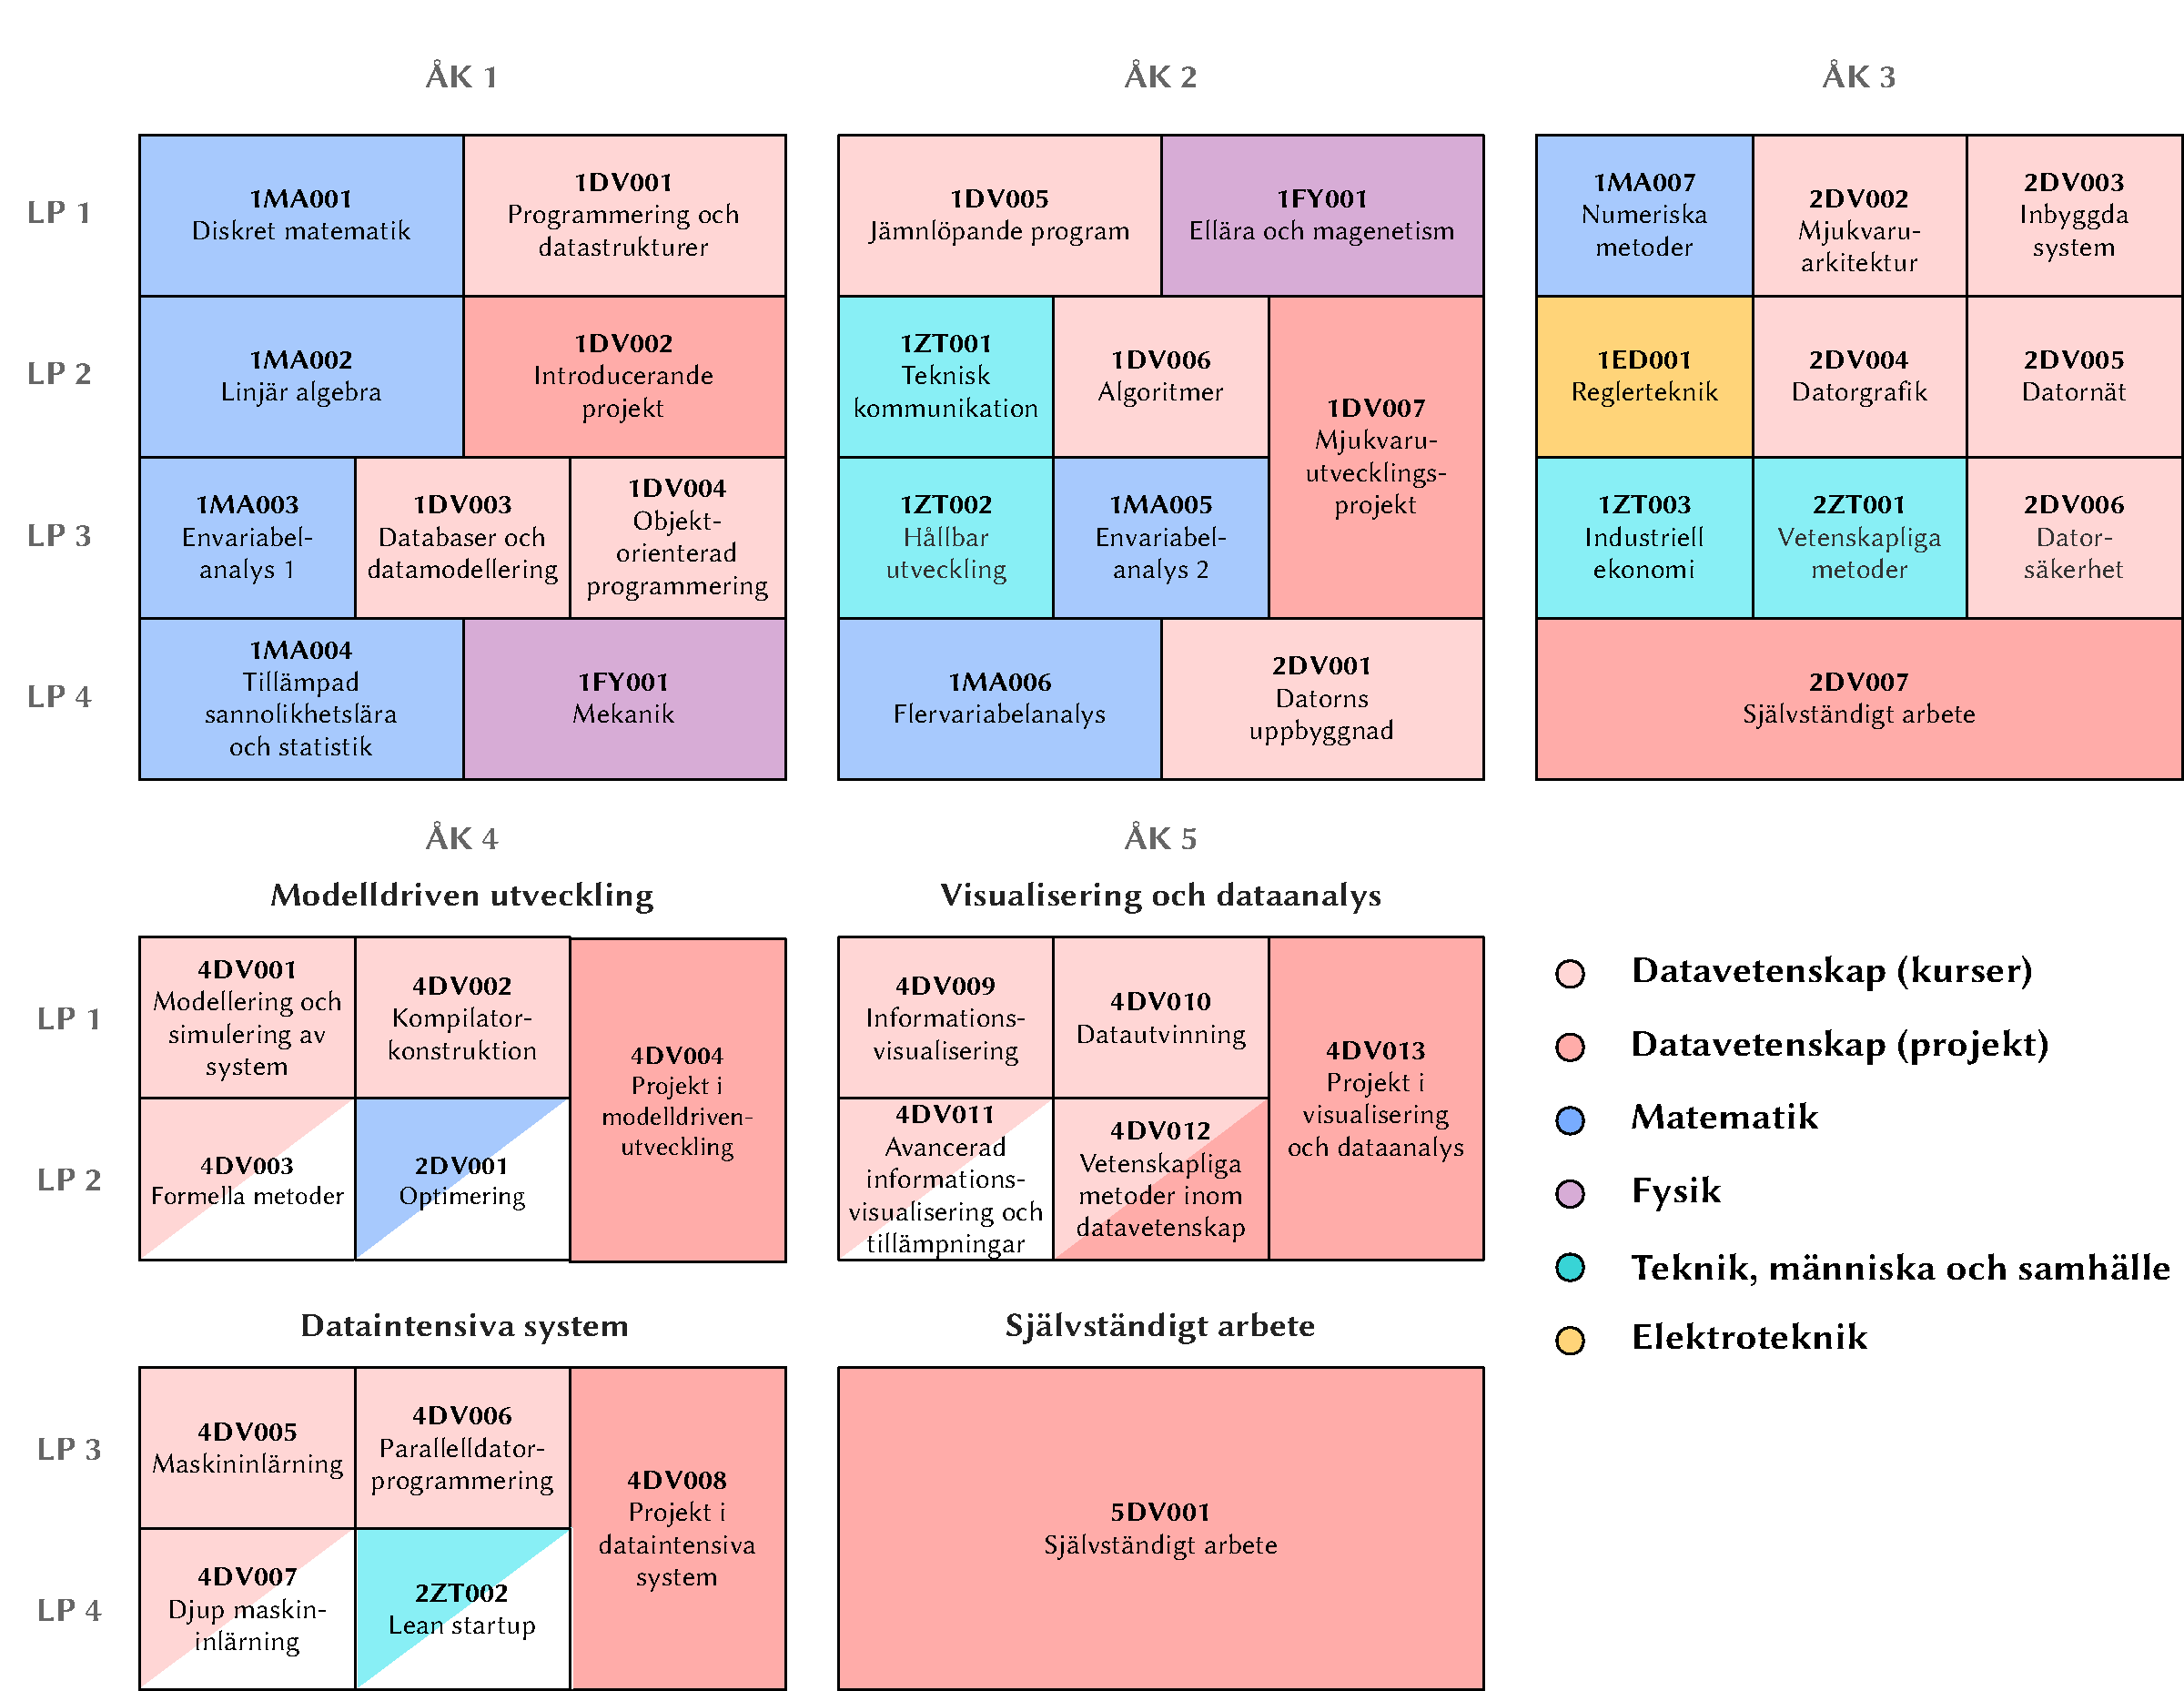
\includegraphics[width=\columnwidth]{images/bs15kk.pdf}
\caption{Programmets upplägg. Varje läsperiod omfattar 15 hp och kurserna omfattar 5, 7,5 eller 10 hp. Det självständiga arbetet i termin 6 omfattar 15 hp och det i termin 10 30 hp. Termin 7--9 består vardera av fyra kurser och ett projekt.}
\end{figure}

\begin{sidewaysfigure}[p]
\centering
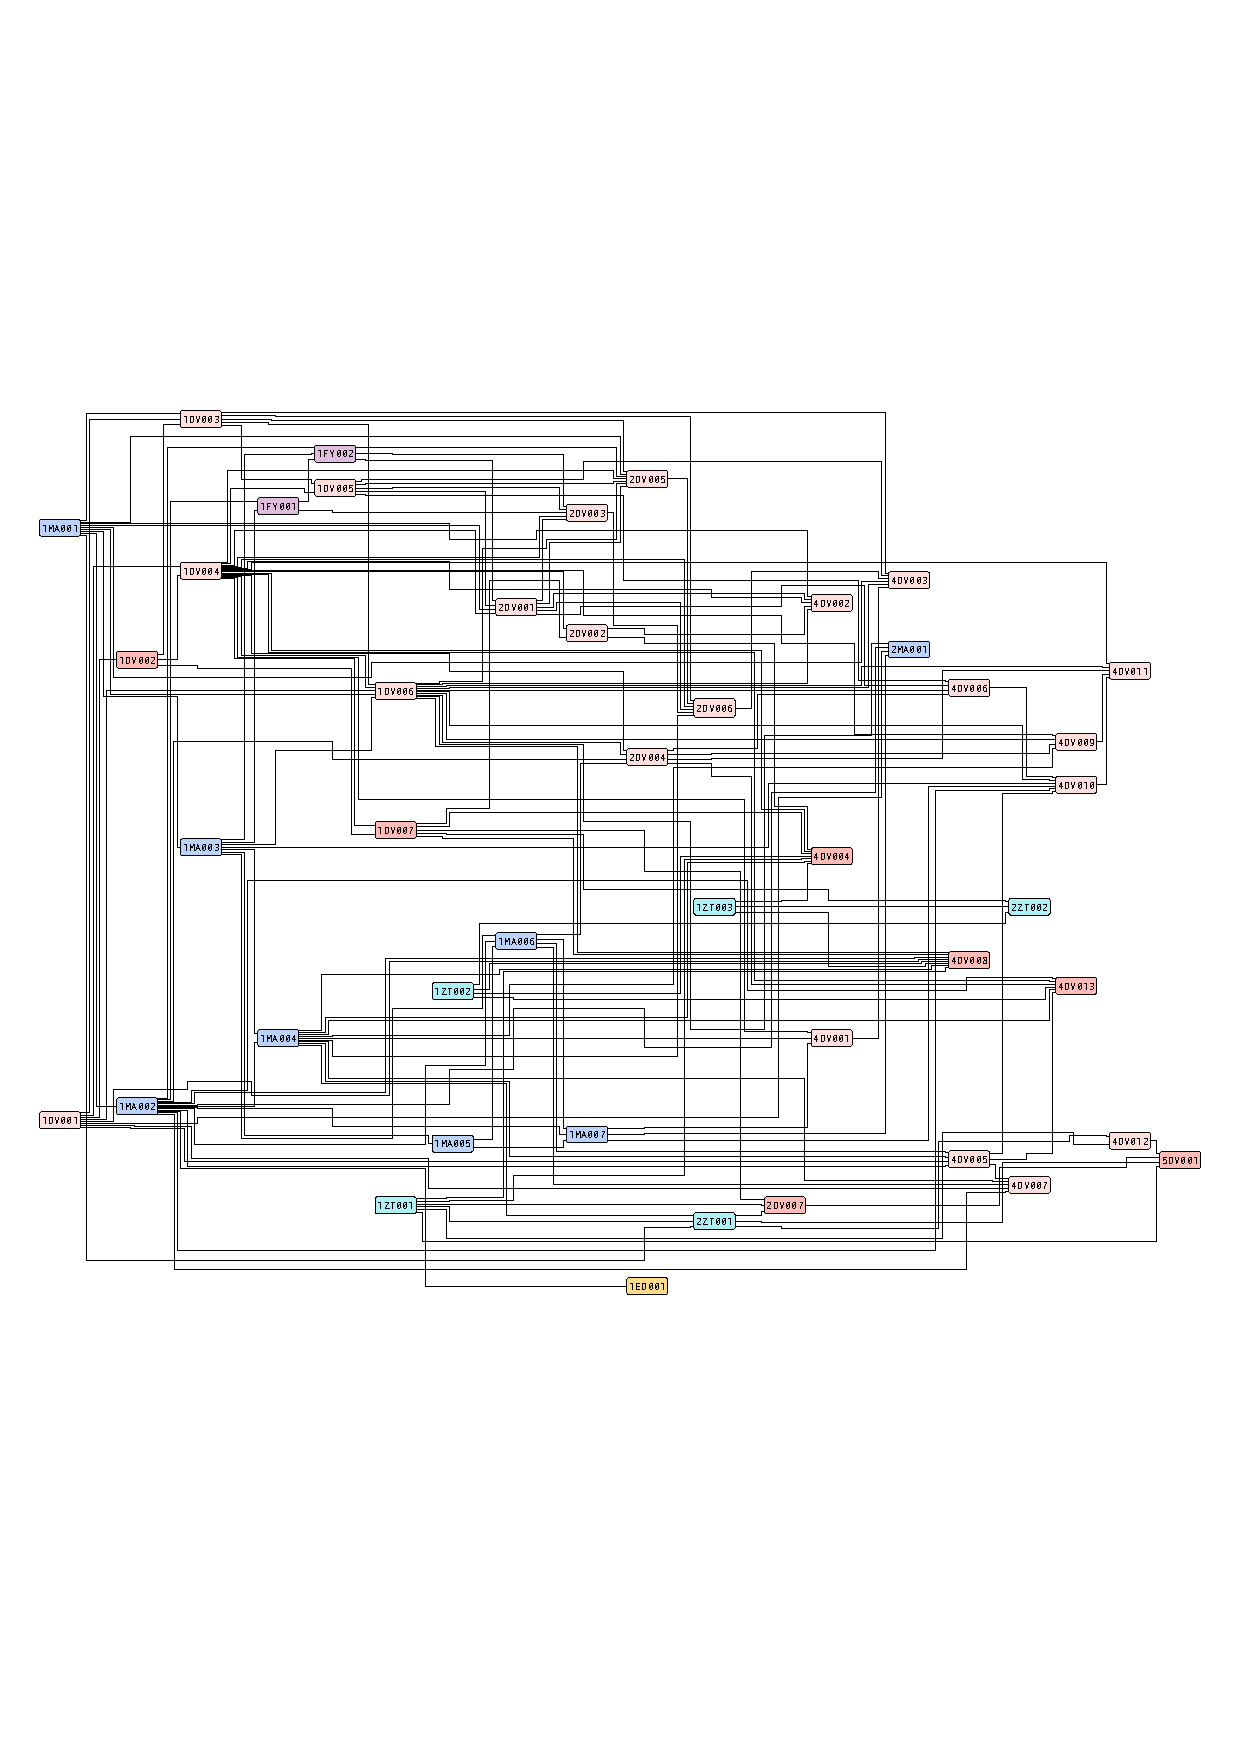
\includegraphics[width=.9\columnwidth]{images/prereq.pdf}
\caption{Förkunskaper.}
\end{sidewaysfigure}


\chapter{Kursplaner}\label{app:kursplaner}

Preliminära kursplaner för samtliga kurser i det föreslagna programmet följer. Varje kursplan är indelad i följande underrubriker. Nivå och och huvudämne, för de kurser som har ett huvudämne anges i början av kursplanen. Observera att de kurskoder som anges är fiktiva och kommer att ändras innan kursplanerna tas. 

\begin{itemize}
	\tightlist
\item Förkunskaper
\item Lärandemål
\item Kursinnehåll
\item Undervisnings- och arbetsformer
\item Examination
\item Måluppfyllelse
\item Kurslitteratur
\item Övrigt
\end{itemize}

Under Förkunskaper anges samtliga kurser som är förkunskaper, oavsett inbördes förkunskaper mellan dessa. Eventuella krav på poäng inom programmet, t.ex. för att få påbörja det självständiga arbetet anges i utbildningsplanen i bilaga~\ref{app:utbplan}.

Måluppfyllelse kopplar samman kursens lärandemål med dess examination. En markering (\faCheck) skall tolkas som att lärandemålet examineras helt eller delvis genom examinationsmomentet. I ansökan används generella namn på examinationsmomenten, t.ex. \texttt{RAP1}. Dessa kommer att ändras till faktiska provmoment när kursplanerna är tagna. Löpnumret används för att särskilja om kursen har flera examinationsmoment av samma typ, t.ex. individuella och gruppinlämningsuppgifter. Vi använder följande typer av examinationsmoment:

\begin{itemize}
\item \texttt{ASK} -- Auskultation på framläggning av andra studenters självständiga arbeten.
\item \texttt{DAT} -- Datortentamen, en tentamen som fokuserar på tekniska färdigheter, t.ex. förmåga att implementera enklare algoritmer i ett programmeringsspråk.
\item \texttt{HEM} -- Hemtentamen, en tentamen som utföras under en eller flera dagar, med full tillgång till kursmaterial, Internet, osv. 
\item \texttt{LAB} -- Laborationsuppgifter, t.ex. programmeringsuppgifter. Redovisas oftast genom en enkel laborationsrapport eller genom att lösningen (t.ex. källkoden) skickas in.
\item \texttt{MUN} -- Muntlig tentamen, en (individuell) tentamen som genomförs muntligt, ofta med hjälp av skrivtavla eller dator. 
\item \texttt{OPP} -- Opponering på en annan students eller grupps inlämning, t.ex. självständigt arbete, projektrapport, osv.
\item \texttt{PRJ} -- Projekt, där arbetet och leverablerna från projektet bedöms, t.ex. arbetet i grupp, hanteringen av vissa moment, osv.
\item \texttt{PRS} -- Presentation, där förmågan att presentera t.ex. muntligt bedöms. 
\item \texttt{RAP} -- Skriftlig rapport där något, t.ex. ett projektarbete rapporteras kring.
\item \texttt{SEM} -- Seminarie och debatt, där aktivt deltagande krävs och bedöms.
\item \texttt{TEN} -- Skriftlig salstentamen. Kan utföras med hjälp av dator.
\item \texttt{UPG} -- Inlämningsuppgift, t.ex. räkneuppgifter eller enklare modelleringsuppgifter. Redovisas oftast genom en enkel rapport.
\end{itemize}

Vi ser en progression mellan typerna, en \texttt{RAP} förväntas vara mera omfattande än en \texttt{UPG} och större fokus läggs vid t.ex. upplägg och struktur. I vissa fall finns en synergi mellan de olika typerna; t.ex. kan \texttt{PRJ} användas för att omfatta mindre projekt, men när projekten växer och större fokus läggs vid t.ex. genomförande kompletteras den med en eller flera \texttt{RAP} som fokuserar på olika aspekter av projektet. \texttt{PRJ} förväntas fortfarande innehålla samtliga leverabler som är viktiga för projektet, t.ex. tidsrapporter. I de fall där olika moment används för triangulering, dvs för att belysa olika aspekter av något eller några moment har stor vikt lags vid att göra det möjligt för en student att vid ett senare tillfälle komplettera eller genomföra examinationen på nytt utan att behöva göra om ett examinationsmoment den redan är godkänd på. 

De olika typerna av tentamen examinerar förutom kursens innehåll något olika aspekter; \texttt{MUN} kan t.ex. testa studentents förmåga att muntligt förklara och resonera sig fram till en lösning, medan \texttt{HEM} kan användas för ämnen som kräver ett större djup i svaren. \texttt{DAT} används främst som ett komplement till \texttt{LAB} och \texttt{UPG}, och ger tillfälle att observera studenten när den löser programmeringsuppgifter samt begränsa vad den har tillgång till, t.ex. med avseende på böcker eller Internet.

Examinationsmomenten kommer att förtydligas i kursernas ``KursPM''.


{\centering\small
\begin{tabular}[]{@{}lllll@{}}
\toprule
\textbf{\textsf{Kod}} & \textbf{\textsf{Benämning}} & \textbf{\textsf{Poäng}} & \textbf{\textsf{Nivå}} & \textbf{\textsf{Huvudområde}} \tabularnewline
\midrule
\texttt{1MA001} & Diskret matematik                                     & 7,5 & G1N & Matematik \tabularnewline     
\texttt{1DV001} & Programmering och datastrukturer                      & 7,5 & G1N & Datavetenskap \tabularnewline 
\texttt{1MA002} & Linjär algebra                                        & 7,5 & G1F & Matematik \tabularnewline     
\texttt{1DV002} & Introducerande projekt                                & 7,5 & G1F & Datavetenskap \tabularnewline 
\texttt{1MA003} & Envariabelanalys 1                                    & 5   & G1F & Matematik \tabularnewline     
\texttt{1DV003} & Databaser och datamodellering                         & 5   & G1F & Datavetenskap \tabularnewline 
\texttt{1DV004} & Objektorienterad programmering                        & 5   & G1F & Datavetenskap \tabularnewline 
\texttt{1MA004} & Tillämpad sannolikhetslära och statistik              & 7,5 & G1F & Matematik \tabularnewline     
\texttt{1FY001} & Mekanik                                               & 7,5 & G1F & Fysik \tabularnewline         
\midrule
\texttt{1DV005} & Jämnlöpande program                                   & 7,5 & G1F & Datavetenskap \tabularnewline 
\texttt{1FY002} & Ellära och magnetism                                  & 7,5 & G1F & Fysik \tabularnewline         
\texttt{1ZT001} & Teknisk kommunikation                                 & 5   & G1N & \tabularnewline           
\texttt{1DV006} & Algoritmer                                            & 5   & G1F & Datavetenskap \tabularnewline 
\texttt{1DV007} & Mjukvaruutvecklingsprojekt                            & 10  & G1F & Datavetenskap \tabularnewline 
\texttt{1ZT002} & Hållbar utveckling                                    & 5   & G1N & \tabularnewline           
\texttt{1MA005} & Envariabelanalys 2                                    & 5   & G1F & Matematik \tabularnewline     
\texttt{1MA006} & Flervariabelanalys                                    & 7,5 & G1F & Matematik \tabularnewline     
\texttt{2DV001} & Datorns uppbyggnad                                    & 7,5 & G2F & Datavetenskap \tabularnewline 
\midrule
\texttt{1MA007} & Numeriska metoder                                     & 5   & G1F & Matematik \tabularnewline     
\texttt{2DV002} & Mjukvaruarkitektur                                    & 5   & G2F & Datavetenskap \tabularnewline 
\texttt{2DV003} & Inbyggda system                                       & 5   & G2F & Datavetenskap \tabularnewline 
\texttt{1ED001} & Reglerteknik                                          & 5   & G1F & Elektroteknik \tabularnewline 
\texttt{2DV004} & Datorgrafik                                           & 5   & G2F & Datavetenskap \tabularnewline 
\texttt{2DV005} & Datornät                                              & 5   & G2F & Datavetenskap \tabularnewline 
\texttt{1ZT003} & Industriell ekonomi                                   & 5   & G1N & \tabularnewline           
\texttt{2ZT001} & Vetenskapliga metoder                                 & 5   & G2F & \tabularnewline               
\texttt{2DV006} & Datorsäkerhet                                         & 5   & G2F & Datavetenskap \tabularnewline 
\texttt{2DV007} & Självständigt arbete                                  & 15  & G2E & Datavetenskap \tabularnewline 
\midrule
\texttt{4DV001} & Modellering och simulering av system                  & 5   & A1N & Datavetenskap \tabularnewline 
\texttt{4DV002} & Kompilatorkonstruktion                                & 5   & A1N & Datavetenskap \tabularnewline 
\texttt{4DV003} & Formella metoder                                      & 5   & A1F & Datavetenskap \tabularnewline 
\texttt{2MA001} & Optimering                                            & 5   & G2F & Matematik \tabularnewline     
\texttt{4DV004} & Projekt i modellbaserad utveckling                    & 10  & A1N & Datavetenskap \tabularnewline 
\texttt{4DV005} & Maskininlärning                                       & 5   & A1N & Datavetenskap \tabularnewline 
\texttt{4DV006} & Parallelldatorprogrammering                           & 5   & A1N & Datavetenskap \tabularnewline 
\texttt{4DV007} & Djup maskininlärning                                  & 5   & A1F & Datavetenskap \tabularnewline 
\texttt{2ZT002} & Lean startup                                          & 5   & G2F &  \tabularnewline 
\texttt{4DV008} & Projekt i dataintensiva system                        & 10  & A1N & Datavetenskap \tabularnewline 
\midrule
\texttt{4DV009} & Informationsvisualisering                             & 5   & A1N & Datavetenskap \tabularnewline 
\texttt{4DV010} & Datautvinning                                         & 5   & A1F & Datavetenskap \tabularnewline 
\texttt{4DV011} & Avancerad informationsvisualisering och tillämpningar & 5   & A1F & Datavetenskap \tabularnewline 
\texttt{4DV012} & Vetenskapliga metoder inom datavetenskap              & 5   & A1F & Datavetenskap \tabularnewline 
\texttt{4DV013} & Projekt i visualisering och dataanalys                & 10  & A1F & Datavetenskap \tabularnewline 
\texttt{5DV001} & Självständigt arbete                                  & 30  & A2E & Datavetenskap \tabularnewline 
\bottomrule
\end{tabular}
}
\pagebreak 

\section*{1MA001 - Diskret matematik (7,5 hp)}

\begin{tabular}{ll}\emph{Huvudområde}: & Datavetenskap\tabularnewline\emph{Fördjupning}: & G1N\tabularnewline\end{tabular}

\subsection*{Förkunskaper}

Grundläggande behörighet samt Matematik D eller Matematik 4
(områdesbehörighet 9/A9).

\subsection*{Lärandemål}

Efter slutförd kurs skall studenten kunna:

\begin{enumerate}
\def\labelenumi{\Alph{enumi}.}
\tightlist
\item
  \emph{Kunskap och förståelse}

  \begin{enumerate}
  \def\labelenumii{\Alph{enumi}.\arabic{enumii}.}
  \tightlist
  \item
    Förklara begrepp i logik, mängdlära, algebra och diskret matematik,
    samt
  \item
    redogöra för definitioner samt formulera och bevisa teorem som är
    centrala i diskret matematik.
  \end{enumerate}
\item
  \emph{Färdighet och förmåga}

  \begin{enumerate}
  \def\labelenumii{\Alph{enumi}.\arabic{enumii}.}
  \tightlist
  \item
    Använda resultat i logik, mängdlära och diskreta matematiska
    modeller,
  \item
    hantera logisk och algebraisk formalism,
  \item
    lösa problem, utföra beräkningar och föra resonemang i diskret
    matematik,
  \item
    skriftligt presentera beräkningar och resonemang inom diskret
    matematik så att de kan följas av den som inte är insatt i
    problemet, samt
  \item
    tillämpa diskreta matematiska modeller på datavetenskapliga problem.
  \end{enumerate}
\item
  \emph{Värderingsförmåga och förhållningssätt}

  \begin{enumerate}
  \def\labelenumii{\Alph{enumi}.\arabic{enumii}.}
  \tightlist
  \item
    Diskutera relevans, räckvidd och noggrannhet av matematiska modeller
    såsom grafer och differensekvationer.
  \end{enumerate}
\end{enumerate}

\subsection*{Kursinnehåll}

Kursen ger en introduktion till diskret matematik, logik och
kombinatorik. Följande moment behandlas:

\begin{itemize}
\tightlist
\item
  Logik: sanningsvärdestabeller, härledningar, disjunktiv och konjunktiv
  normalform, satslogik, predikatlogisk formalism.
\item
  Mängdlära: dualitetsprincipen, de Morgans lagar, principen för
  inklusion och exklusion.
\item
  Boolesk algebra.
\item
  Relationer och funktioner: funktionslära, egenskaper hos relationer,
  ekvivalensrelationer, ordningsrelationer, matris- och
  grafrepresentation av relationer.
\item
  Induktion: välordningsprincipen, matematisk induktion, rekursion.
\item
  Genererande funktioner.
\item
  Modulär aritmetik.
\item
  Kombinatorik.
\item
  Differensekvationer.
\item
  Grafteori: Eulerkretsar, Hamiltonbanor, plana grafer, färgläggning av
  grafer och kromatiska polynom, träd.
\end{itemize}

\subsection*{Undervisnings- och arbetsformer}

Föreläsningar, lärarledda räkneövningar och lärarledda möten relaterade
till inlämningsuppgifterna.

\subsection*{Examination}

Examinationen av kursen delas in i följande moment:

\begin{longtable}[]{@{}llcc@{}}
\toprule
\textsf{Kod} & \textsf{Benämning} & \textsf{Betyg} & \textsf{Poäng}\tabularnewline
\midrule
\endhead
\texttt{TEN1} & Tentamen: Problemlösning & A-F & 5\tabularnewline
\texttt{TEN2} & Tentamen: Teori & G-U & 1,5\tabularnewline
\texttt{UPG1} & Inlämningsuppgift & G-U & 1,0\tabularnewline
\bottomrule
\end{longtable}

För godkänt betyg på kursen krävs minst betyg E på \texttt{TEN1} samt betyg G på
\texttt{TEN2} och \texttt{UPG1}. Slutbetyget bestäms från \texttt{TEN1}.

\subsection*{Måluppfyllelse}

Examinationsmomenten kopplas till lärandemålen enligt följande:

\begin{longtable}[]{@{}lccc@{}}
\toprule
\textsf{Lärandemål} & \texttt{TEN1} & \texttt{TEN2} & \texttt{UPG1}\tabularnewline
\midrule
\endhead
A.1 & & \faCheck &\tabularnewline
A.2 & & \faCheck &\tabularnewline
B.1 & \faCheck & &\tabularnewline
B.2 & \faCheck & &\tabularnewline
B.3 & \faCheck & \faCheck &\tabularnewline
B.4 & \faCheck & & \faCheck\tabularnewline
B.5 & & & \faCheck\tabularnewline
C.1 & & & \faCheck\tabularnewline
\bottomrule
\end{longtable}

\subsection*{Kurslitteratur}

Obligatorisk litteratur:

\begin{itemize}
\tightlist
\item
  Rosen, K H, \emph{Discrete mathematics and its applications},
  McGraw-Hill, 2012. Antal sidor: 250 av 1024.
\end{itemize}

\subsection*{Övrigt}

Kursen genomförs på ett sätt sådant att både kvinnor och mäns kunskap och erfarenhet utvecklas och görs synlig.
\pagebreak

\section*{1DV001 - Programmering och datastrukturer (7,5 hp)}

\begin{tabular}{ll}\emph{Huvudområde}: & Datavetenskap\tabularnewline\emph{Fördjupning}: & G1N\tabularnewline\end{tabular}

\subsection*{Förkunskaper}

Grundläggande behörighet samt Matematik D eller Matematik 4
(områdesbehörighet 9/A9).

\subsection*{Lärandemål}

Efter slutförd kurs skall studenten kunna:

\begin{enumerate}
\def\labelenumi{\Alph{enumi}.}
\tightlist
\item
  \emph{Kunskap och förståelse}

  \begin{enumerate}
  \def\labelenumii{\Alph{enumi}.\arabic{enumii}.}
  \tightlist
  \item
    Förklara grundläggande programspråkskonstruktioner som t.ex.
    variabler, typer, styrande satser och funktioner, samt
  \item
    förklara grundläggande algoritmer och datastrukturer, samt
    exemplifiera hur och när de bör användas.
  \end{enumerate}
\item
  \emph{Färdighet och förmåga}

  \begin{enumerate}
  \def\labelenumii{\Alph{enumi}.\arabic{enumii}.}
  \tightlist
  \item
    Skapa och implementera en lösning till ett givet problem i
    programmeringsspråket Python,
  \item
    implementera givna algoritmer för att lösa kända typer av problem
    (t.ex. sortering och sökning) och analysera deras tidskomplexitet,
  \item
    installera och använda verktyg och bibliotek som används vid
    programmering,
  \item
    strukturera och genomföra korta muntliga och skriftliga
    presentationer av mindre programmeringsprojekt, samt
  \item
    dokumentera program och följa programkodskonventioner.
  \end{enumerate}
\item
  \emph{Värderingsförmåga och förhållningssätt}

  \begin{enumerate}
  \def\labelenumii{\Alph{enumi}.\arabic{enumii}.}
  \tightlist
  \item
    Resonera kring hur välstrukturerat och lättförstått ett program är,
    samt
  \item
    göra att motiverat val av datastrukturer och algoritmer i olika
    scenarier, t.ex. med avseende på prestanda.
  \end{enumerate}
\end{enumerate}

\subsection*{Kursinnehåll}

Kursen är en inledande programmeringskurs i programspråket Python.
Kursens första del fokuserar på programmeringsfärdigheter och vanliga
programspråkskonstruktioner (t.ex. variabler, typer, styrande satser och
funktioner). Under kursens andra halva introduceras algoritmer och
datastrukturer med exempel från t.ex. sökning och sortering. Egenskap
hos och analys av dessa, t.ex. med avseende på tidskomplexitet
diskuteras.

Följande moment behandlas:

\begin{itemize}
\tightlist
\item
  Introduktion till labbmiljön och andra resurser, t.ex. lärplattformen.
\item
  En dators uppbyggnad och hur program exekveras.
\item
  Introduktion till utvecklingsmiljöer, t.ex. editor, interpretator,
  osv.
\item
  Problemlösning.
\item
  Att formulera lösningar på problem så att datorer kan hantera dem.
\item
  Grundläggande programspråkskonstruktioner.
\item
  Filhantering.
\item
  Att använda externa programvarubibliotek.
\item
  Att använda klasser, objekt och moduler.
\item
  Vanliga datastrukturer (t.ex. listor, mängder, tabeller och träd).
\item
  Vanliga algoritmer för sökning och sortering.
\item
  Enkla uppskattningar av bästa, värsta och genomsnittlig
  tidskomplexitet.
\item
  Dokumentation av kod och kodkonventioner.
\item
  Parvist arbete, problemlösning och kommunikationsfärdigheter.
\end{itemize}

\subsection*{Undervisnings- och arbetsformer}

Undervisningen sker i form av föreläsningar, lärarledda laborationer,
projekt med regelbundna handledning. Kursen avslutas med en muntlig och
skriftlig projektredovisning. Laborationerna är individuella, projekt
och presentationer sker i par.

\subsection*{Examination}

Examinationen av kursen delas in i följande moment:

\begin{longtable}[]{@{}llcc@{}}
\toprule
\textsf{Kod} & \textsf{Benämning} & \textsf{Betyg} & \textsf{Poäng}\tabularnewline
\midrule
\endhead
\texttt{LAB1} & Programmeringsuppgifter & A-F & 3\tabularnewline
\texttt{DAT1} & Datortentamen & G-U & 1\tabularnewline
\texttt{PRJ1} & Projekt i algoritmer och datastrukturer & A-F &
3,5\tabularnewline
\bottomrule
\end{longtable}

För godkänt betyg på kursen krävs betyg G på \texttt{DAT1} och minst betyg E på
övriga moment. Slutbetyget bestäms från: \texttt{LAB1} (50~\%) och \texttt{PRJ1} (50~\%).

\subsection*{Måluppfyllelse}

Examinationsmomenten kopplas till lärandemålen enligt följande:

\begin{longtable}[]{@{}lccc@{}}
\toprule
\textsf{Lärandemål} & \texttt{LAB1} & \texttt{DAT1} & \texttt{PRJ1}\tabularnewline
\midrule
\endhead
A.1 & \faCheck & \faCheck &\tabularnewline
A.2 & \faCheck & \faCheck & \faCheck\tabularnewline
B.1 & \faCheck & \faCheck & \faCheck\tabularnewline
B.2 & \faCheck & \faCheck & \faCheck\tabularnewline
B.3 & \faCheck & & \faCheck\tabularnewline
B.4 & & & \faCheck\tabularnewline
B.5 & \faCheck & & \faCheck\tabularnewline
C.1 & \faCheck & &\tabularnewline
C.2 & & & \faCheck\tabularnewline
\bottomrule
\end{longtable}

\subsection*{Kurslitteratur}

Obligatorisk litteratur:

\begin{itemize}
\tightlist
\item
  Zelle, J. M., \emph{Python Programming: An Introduction to Computer
  Science}, tredje utgåvan, Franklin, Beedle \& Associates, 2016. Antal
  sidor: 450 av 812.
\end{itemize}

\subsection*{Övrigt}

Kursen genomförs på ett sätt sådant att både kvinnor och mäns kunskap och erfarenhet utvecklas och görs synlig.
\pagebreak

\section*{1MA002 - Linjär algebra (7,5 hp)}

\begin{tabular}{ll}\emph{Huvudområde}: & Matematik\tabularnewline\emph{Fördjupning}: & G1F\tabularnewline\end{tabular}

\subsection*{Förkunskaper}

\begin{itemize}
\tightlist
\item
  1MA001 - Diskret matematik
\end{itemize}

\subsection*{Lärandemål}

Efter slutförd kurs skall studenten kunna:

\begin{enumerate}
\def\labelenumi{\Alph{enumi}.}
\tightlist
\item
  \emph{Kunskap och förståelse}

  \begin{enumerate}
  \def\labelenumii{\Alph{enumi}.\arabic{enumii}.}
  \tightlist
  \item
    Redogöra för linjära algebrans grundläggande begrepp och
    operationer, kunna utföra dessa operationer och utnyttja detta i
    problemlösning, samt
  \item
    redogöra för sambanden mellan linjära algebrans grundläggande
    begrepp och utnyttja dessa samband i problemlösning.
  \end{enumerate}
\item
  \emph{Färdighet och förmåga}

  \begin{enumerate}
  \def\labelenumii{\Alph{enumi}.\arabic{enumii}.}
  \tightlist
  \item
    Kombinera kunskaper om olika begrepp, operationer och metoder från
    linjära algebran i problemlösning,
  \item
    redogöra för matematiska resonemang på ett strukturerat och logiskt
    sammanhängande sätt, samt
  \item
    använda programspråket Matlab i problemlösning.
  \end{enumerate}
\item
  \emph{Värderingsförmåga och förhållningssätt}

  \begin{enumerate}
  \def\labelenumii{\Alph{enumi}.\arabic{enumii}.}
  \tightlist
  \item
    Visa förmåga att bedöma rimligheten i resultat av beräkningar.
  \end{enumerate}
\end{enumerate}

\subsection*{Kursinnehåll}

Det övergripande syftet med kursen är att ge en sammanhållen begreppsram
från linjär algebra med tillämpningar inom analys, grafteori,
datorgrafik, mekanik, numerisk analys, matematisk statistik,
reglerteknik, ekonomi och linjär optimering m.fl. ämnen.

\begin{itemize}
\tightlist
\item
  Linjära ekvationssystem.
\item
  Geometriska vektorer, räta linjer och plan.\\
\item
  Linjära rum, euklidiska rum, koordinatsystem, underrum, linjärt
  oberoende, baser, basbyte, skalärprodukt, ortogonalitet,
  vektorprodukt, volymfunktion.
\item
  Matriser: Matrisalgebra, invers matris och linjära ekvationssystem,
  determinant, rang, egenvärde, egenvektor och diagonalisering.
\item
  Linjära avbildningar: Matrisframställnig, nollrum, värderum,
  dimensionssatsen.
\item
  Tillämpningar på projektioner, speglingar och rotationer.
\item
  Introduktion till minsta kvadratmetoden. Gram-Schmidts
  ortogonaliseringsmetod.
\item
  Linjära algebrans tillämpningar inom diskret matematik, analys,
  teknik, fysik och ekonomi.
\item
  Problemlösning med hjälp av programvaran Matlab.
\end{itemize}

\subsection*{Undervisnings- och arbetsformer}

Undervisningen sker i form av föreläsningar, lärarledda räkneövningar
och datorlaborationer. Inlämningsuppgifter sker i par. Obligatorisk
närvaro kan förekomma på vissa moment.

\subsection*{Examination}

Examinationen av kursen delas in i följande moment:

\begin{longtable}[]{@{}llcc@{}}
\toprule
\textsf{Kod} & \textsf{Benämning} & \textsf{Betyg} & \textsf{Poäng}\tabularnewline
\midrule
\endhead
\texttt{LAB1} & Laborationer i Matlab & A-F & 1,5\tabularnewline
\texttt{TEN1} & Skriftlig tentamen & A-F & 6\tabularnewline
\bottomrule
\end{longtable}

För godkänt betyg på kursen krävs minst betyg E på samtliga moment.
Slutbetyget bestäms från: \texttt{LAB1} (20~\%) och \texttt{TEN1} (80~\%).

\subsection*{Måluppfyllelse}

Examinationsmomenten kopplas till lärandemålen enligt följande:

\begin{longtable}[]{@{}lcc@{}}
\toprule
\textsf{Lärandemål} & \texttt{LAB1} & \texttt{TEN1}\tabularnewline
\midrule
\endhead
A.1 & \faCheck & \faCheck\tabularnewline
A.2 & \faCheck & \faCheck\tabularnewline
B.1 & \faCheck & \faCheck\tabularnewline
B.2 & \faCheck & \faCheck\tabularnewline
B.3 & \faCheck &\tabularnewline
C.1 & \faCheck & \faCheck\tabularnewline
\bottomrule
\end{longtable}

\subsection*{Kurslitteratur}

Obligatorisk litteratur:

\begin{itemize}
\tightlist
\item
  Lindstöm, T., \emph{Med fokus på linjär algebra}, tredje upplagan,
  Studentlitteratur, 2017. Antal sidor: 270 av 336.
\end{itemize}

\subsection*{Övrigt}

Kursen genomförs på ett sätt sådant att både kvinnor och mäns kunskap och erfarenhet utvecklas och görs synlig.
\pagebreak

\section*{1DV002 - Introducerande projekt (7,5 hp)}

\begin{tabular}{ll}\emph{Huvudområde}: & Datavetenskap\tabularnewline\emph{Fördjupning}: & G1F\tabularnewline\end{tabular}

\subsection*{Förkunskaper}

\begin{itemize}
\tightlist
\item
  1DV001 - Programmering och datastrukturer
\end{itemize}

\subsection*{Lärandemål}

Efter slutförd kurs skall studenten kunna:

\begin{enumerate}
\def\labelenumi{\Alph{enumi}.}
\tightlist
\item
  \emph{Kunskap och förståelse}

  \begin{enumerate}
  \def\labelenumii{\Alph{enumi}.\arabic{enumii}.}
  \tightlist
  \item
    Namnge och förklara funktionen hos de viktigaste komponenterna i en
    Raspberry Pi,
  \item
    förklara hur man skriver, installerar och exekverar Python-program
    på en Raspberry Pi,
  \item
    förklara hur systemkrav tas fram, specificeras och testas,
  \item
    översiktligt redogöra för vad projektledning och kvalitetsarbete
    innebär i praktiken, samt
  \item
    redogöra för mjukvaruindustrins olika sektorer och olika
    arbetsuppgifter.
  \end{enumerate}
\item
  \emph{Färdighet och förmåga}

  \begin{enumerate}
  \def\labelenumii{\Alph{enumi}.\arabic{enumii}.}
  \tightlist
  \item
    Utveckla Pythonprogram för Raspberry Pi med externa enheter (t.ex.
    sensorer) och nätverkskoppling,
  \item
    analysera ett problem, skapa en kravspecifikation, designa och
    implementera lösningar, och verifiera att lösningen uppfyller alla
    krav,
  \item
    använda vanliga tekniska projektverktyg (tex versionshantering med
    Git),
  \item
    självständigt söka efter och värdera information,
  \item
    strukturera och genomföra en skriftlig och muntlig presentation av
    genomförda laborationer och projekt, samt
  \item
    genomföra ett projekt i grupp under begränsad tid och där tillämpa
    en arbetsform som presenterats i kursen.
  \end{enumerate}
\item
  \emph{Värderingsförmåga och förhållningssätt}

  \begin{enumerate}
  \def\labelenumii{\Alph{enumi}.\arabic{enumii}.}
  \tightlist
  \item
    Reflektera över och värdera en given ansats att lösa ett problem,
  \item
    reflektera över relationen mellan ämneskunskap, ingenjörsfärdigheter
    och yrkesrollen ingenjör, samt
  \item
    reflektera över och värdera sin egen kontra gruppens insats vid
    laborations- och projektarbete.
  \end{enumerate}
\end{enumerate}

\subsection*{Kursinnehåll}

Kursen har två parallella spår: Det första introducerar kort Internet of
Things och det introducerar studenten till yrkesrollen samt fördjupas
dess ämneskunskaper. Inom det första spåret presentation en enkel dator,
Raspberry Pi, och hur man kan skriva program i Python som interagerar
med externa enheter, sensorer och tjänster över Internet. Inom det andra
spåret introduceras hur man arbetar i projekt och grupp, samt
yrkesrollen (mjukvaru)ingenjör.

Följande moment behandlas:

\begin{itemize}
\tightlist
\item
  Introduktion till Internet of Things.
\item
  Introduktion till Raspberry Pi (hårdvara och mjukvara).
\item
  Implementera och exekvera Pythonprogram på Raspberry Pi.
\item
  Interagera med externa enheter (t.ex. sensorer).
\item
  Interagera med nätverkskopplade enheter/Internet.
\item
  Fördjupning av labbmiljön.
\item
  Introduktion till kravhantering, mjukvarudesign och testning.
\item
  Introduktion av verktyg och metoder som används inom ett projekt,
  t.ex. versionshantering, kravhantering, kommunikation, osv..
\item
  Projektmetodik och projektdynamik.
\item
  Hur man arbetar i grupp, vilka roller som finns, vilket ansvar
  individen har, osv.
\item
  Informationssökning.
\item
  Hur man skriver enklare projektdokumentation.
\item
  Muntlig presentation av tekniskt material.
\item
  Skriftlig presentation av tekniskt material.
\item
  Ingenjörens yrkesroll, arbetsuppgifter och förhållningssätt.
\item
  Ingenjörens ansvar och arbetsmiljö.
\end{itemize}

\subsection*{Undervisnings- och arbetsformer}

Undervisningen sker i form av föreläsningar, lärarledda laborationer,
handledning i projektgrupp och en slutpresentation. Laborationerna sker
i par och projekt och presentationer sker i grupper om 4 studenter.
Yrkesrollen ingenjör presenteras via gästföreläsningar och/eller
studiebesök.

\subsection*{Examination}

Examinationen av kursen delas in i följande moment:

\begin{longtable}[]{@{}llcc@{}}
\toprule
\textsf{Kod} & \textsf{Benämning} & \textsf{Betyg} & \textsf{Poäng}\tabularnewline
\midrule
\endhead
\texttt{LAB1} & Programmeringsuppgifter & G-U & 1,5\tabularnewline
\texttt{PRJ1} & Projekt & A-F & 4\tabularnewline
\texttt{PRS1} & Presentation & A-F & 1\tabularnewline
\texttt{UPG1} & Uppgifter om yrkesrollen ingenjör & G-U & 1\tabularnewline
\bottomrule
\end{longtable}

För godkänt betyg på kursen krävs betyg G på \texttt{LAB1} och \texttt{UPG1} samt minst
betyg E på övriga moment. Slutbetyget bestäms från: \texttt{PRJ1} (75~\%) och \texttt{PRS1}
(25~\%).

\subsection*{Måluppfyllelse}

Examinationsmomenten kopplas till lärandemålen enligt följande:

\begin{longtable}[]{@{}lcccc@{}}
\toprule
\textsf{Lärandemål} & \texttt{LAB1} & \texttt{PRJ1} & \texttt{PRS1} & \texttt{UPG1}\tabularnewline
\midrule
\endhead
A.1 & \faCheck & & &\tabularnewline
A.2 & \faCheck & & &\tabularnewline
A.3 & & \faCheck & \faCheck &\tabularnewline
A.4 & & \faCheck & \faCheck & \faCheck\tabularnewline
A.5 & & & & \faCheck\tabularnewline
B.1 & \faCheck & \faCheck & &\tabularnewline
B.2 & & \faCheck & \faCheck &\tabularnewline
B.3 & & \faCheck & &\tabularnewline
B.4 & \faCheck & \faCheck & &\tabularnewline
B.5 & \faCheck & & \faCheck &\tabularnewline
B.6 & & & \faCheck &\tabularnewline
C.1 & & \faCheck & \faCheck &\tabularnewline
C.2 & & & \faCheck & \faCheck\tabularnewline
C.3 & \faCheck & \faCheck & &\tabularnewline
\bottomrule
\end{longtable}

\subsection*{Kurslitteratur}

Kurslitteratur bestäms i samråd med handledare.

\subsection*{Övrigt}

Kursen genomförs på ett sätt sådant att både kvinnor och mäns kunskap och erfarenhet utvecklas och görs synlig.
\pagebreak

\section*{1MA003 - Envariabelanalys 1 (5 hp)}

\begin{tabular}{ll}\emph{Huvudområde}: & Matematik\tabularnewline\emph{Fördjupning}: & G1F\tabularnewline\end{tabular}

\subsection*{Förkunskaper}

\begin{itemize}
\tightlist
\item
  1MA001 - Diskret matematik
\end{itemize}

\subsection*{Lärandemål}

Efter slutförd kurs skall studenten kunna:

\begin{enumerate}
\def\labelenumi{\Alph{enumi}.}
\tightlist
\item
  \emph{Kunskap och förståelse}

  \begin{enumerate}
  \def\labelenumii{\Alph{enumi}.\arabic{enumii}.}
  \tightlist
  \item
    Förklara analytiska begrepp såsom gränsvärden och kontinuitet, samt
  \item
    redogöra för definitioner samt formulera och bevisa teorem som är
    centrala i analys, såsom medelvärdessatsen och analysens huvudsats.
  \end{enumerate}
\item
  \emph{Färdighet och förmåga}

  \begin{enumerate}
  \def\labelenumii{\Alph{enumi}.\arabic{enumii}.}
  \tightlist
  \item
    Hantera elementära funktioner algebraiskt och analytiskt,
  \item
    använda differential- och integralkalkyl i en variabel,
  \item
    lösa problem, utföra beräkningar och föra resonemang i analys,
  \item
    skriftligt presentera beräkningar och resonemang så att de kan
    följas av den som inte är insatt i problemet,
  \item
    tillämpa differential- och integralkalkyl på tekniska, fysikaliska
    och datavetenskapliga problem, samt
  \item
    visualisera resultat såsom grafer till funktioner.
  \end{enumerate}
\item
  \emph{Värderingsförmåga och förhållningssätt}

  \begin{enumerate}
  \def\labelenumii{\Alph{enumi}.\arabic{enumii}.}
  \tightlist
  \item
    Diskutera relevans, räckvidd och noggrannhet av matematiska modeller
    såsom differentialekvationer.
  \end{enumerate}
\end{enumerate}

\subsection*{Kursinnehåll}

Kursen ger en introduktion till envariabelanalys. Följande moment
behandlas:

\begin{itemize}
\tightlist
\item
  Gränsvärden och kontinuitet: gränsvärdesdefinitionen, räkneregler,
  instängningssatsen, standardgränsvärden, talet e.
\item
  Derivata och funktionsstudier: derivatans definition, räkneregler, de
  elementära funktionernas derivator, medelvärdessatsen,
  extremvärdesproblem, kurvritning, asymptoter.
\item
  Integraler: primitiva funktioner, integralens definition, analysens
  huvudsats, integralkalkylens medelvärdessats, partiell integration,
  variabelbyte, integrering av rationella funktioner.
\item
  Differentialekvationer: linjära och separabla ekvationer av första
  ordningen, linjära ekvationer av andra ordningen med konstanta
  koefficienter.
\item
  Matematisk modellering med differentialekvationer.
\end{itemize}

\subsection*{Undervisnings- och
arbetsformer}

Föreläsningar och lärarledda räkneövningar.

\subsection*{Examination}

Examinationen av kursen delas in i följande moment:

\begin{longtable}[]{@{}llcc@{}}
\toprule
\textsf{Kod} & \textsf{Benämning} & \textsf{Betyg} & \textsf{Poäng}\tabularnewline
\midrule
\endhead
\texttt{TEN1} & Tentamen: Problemlösning & A-F & 4\tabularnewline
\texttt{TEN2} & Tentamen: Teori & G-U & 1\tabularnewline
\bottomrule
\end{longtable}

För godkänt betyg på kursen krävs minst betyg E på \texttt{TEN1} samt betyg G på
\texttt{TEN2}. Slutbetyget bestäms från \texttt{TEN1}.

\subsection*{Måluppfyllelse}

Examinationsmomenten kopplas till lärandemålen enligt följande:

\begin{longtable}[]{@{}lcc@{}}
\toprule
\textsf{Lärandemål} & \texttt{TEN1} & \texttt{TEN2}\tabularnewline
\midrule
\endhead
A.1 & & \faCheck\tabularnewline
A.2 & & \faCheck\tabularnewline
B.1 & \faCheck &\tabularnewline
B.2 & \faCheck &\tabularnewline
B.3 & \faCheck & \faCheck\tabularnewline
B.4 & \faCheck &\tabularnewline
B.5 & \faCheck &\tabularnewline
B.6 & \faCheck &\tabularnewline
C.1 & \faCheck &\tabularnewline
\bottomrule
\end{longtable}

\subsection*{Kurslitteratur}

Obligatorisk litteratur:

\begin{itemize}
\tightlist
\item
  Månsson, J. och Nordbeck, P., \emph{Endimensionell analys},
  Studentlitteratur, 2011. Antal sidor: 200 av 400.
\item
  Månsson, J. och Nordbeck, P., \emph{Övningar i endimensionell analys},
  Studentlitteratur, 2011. Antal sidor: 100 av 206.
\end{itemize}

\subsection*{Övrigt}

Kursen genomförs på ett sätt sådant att både kvinnor och mäns kunskap och erfarenhet utvecklas och görs synlig.
\pagebreak
\section*{1DV003 - Databaser och datamodellering (5 hp)}

\begin{tabular}{ll}\emph{Huvudområde}: & Datavetenskap\tabularnewline\emph{Fördjupning}: & G1F\tabularnewline\end{tabular}

\subsection*{Förkunskaper}

\begin{itemize}
\tightlist
\item
  1DV001 - Programmering och datastrukturer
\item
  1DV002 - Introducerande projekt
\item
  1MA001 - Diskret matematik
\end{itemize}

\subsection*{Lärandemål}

Efter slutförd kurs skall studenten kunna:

\begin{enumerate}
\def\labelenumi{\Alph{enumi}.}
\tightlist
\item
  \emph{Kunskap och förståelse}

  \begin{enumerate}
  \def\labelenumii{\Alph{enumi}.\arabic{enumii}.}
  \tightlist
  \item
    Förklara de grundläggande begreppen relaterade till datorbaserade
    informationssystem samt förklara de viktigaste problemen och
    regelverken i samband med datahantering i stora organisationer och
    företag,
  \item
    översiktligt redogöra för olika databastyper, t.ex. relations-,
    dokument- och objekt-baserade,
  \item
    förklara de olika typerna av modeller (konceptuell, logisk och
    fysisk) som används för att ta fram och resonera kring en databas,
  \item
    förklara relationsmodellen, relationsalgebra, kopplingen till
    predikatlogik och normalformer, samt
  \item
    redogöra för hur data, t.ex. tabeller, kan lagras på block-enheter,
    t.ex. hårddiskar, inklusive att kunna beskriva de algoritmer och
    datastrukturer som behövs.
  \end{enumerate}
\item
  \emph{Färdighet och förmåga}

  \begin{enumerate}
  \def\labelenumii{\Alph{enumi}.\arabic{enumii}.}
  \tightlist
  \item
    Utforma datamodeller på olika semantiska nivåer (begreppsmässig,
    logisk, fysisk) med hjälp av lämplig formalism, såsom
    Entity-Relationship och relationsmodeller,
  \item
    optimera en databasdesign genom att använda normalformer (1NF, 2NF,
    3NF, BCNF), med beaktande av egenskaperna hos de fysiska medier som
    används för datalagring, samt
  \item
    implementera relationsdatamodeller i en databashanterare samt skapa,
    fråga och manipulera data med hjälp av SQL via klientprogram och
    program implementerade i Python.
  \end{enumerate}
\item
  \emph{Värderingsförmåga och förhållningssätt}

  \begin{enumerate}
  \def\labelenumii{\Alph{enumi}.\arabic{enumii}.}
  \tightlist
  \item
    Analysera och värdera en domän och dess begränsningar som en
    datamodell samt muntligt och skriftligt diskutera fördelarna och
    nackdelarna med designen,
  \item
    reflektera över egenskaperna hos olika datamodeller och välja de som
    är mest lämpade för det problem som ska lösas, samt
  \item
    resonera om hur olika designalternativ påverkar databasens
    egenskaper, t.ex. prestanda och möjliga frågor.
  \end{enumerate}
\end{enumerate}

\subsection*{Kursinnehåll}

Kursen ger en introduktion till databaser och
informationshanteringssystem. Den utgår från grunderna i hur data kan
lagras, t.ex. via relationsmodellen eller via nätverksmodeller och
diskuterar hur frågespråk kan byggas ovanpå dessa. Bra design diskuteras
på flera olika nivåer, från logiska datamodeller, till t.ex.
relationsmodellen och normalformer och den faktiska fysiska lagringen.

Följande moment behandlas:

\begin{itemize}
\tightlist
\item
  Introduktion till datorbaserade informationshanteringssystem.
\item
  Vikten av databaser och informationshantering i samhället.
\item
  Vilken data kan, får och bör lagras. Vilka regelverk gäller, t.ex.
  GDPR.
\item
  Konceptuella, logiska och fysiska datamodeller.
\item
  Olika typer av databashanterare.
\item
  Diagram för att modellera data, t.ex. E/R.
\item
  Relationsmodeller och relationsalgebra.
\item
  Databasfrågor och databasmanipulation med SQL.
\item
  Funktionella beroenden och normalformer (1NF, 2NF, 3NF, BCNF).
\item
  Installation och användning av vanliga databashanterare, t.ex. MySQL i
  labbmiljön.
\item
  Utveckling av program som använder en databas.
\item
  Predikatlogik och dess relation till databaser.
\item
  Introduktion till samtidighet, låsning och hur transaktioner fungerar.
\item
  Filsystem och hur data lagras på blockenheter (t.ex. hårddiskar).
\end{itemize}

\subsection*{Undervisnings- och
arbetsformer}

Undervisningen sker i form av föreläsningar, lärarledda laborationer och
handledning av inlämningsuppgifter. Laborationer och inlämningsuppgifter
sker i par. I vissa moment av kursen förväntas studenten att på egen
hand söka den information som behövs för att lösa en uppgift.

\subsection*{Examination}

Examinationen av kursen delas in i följande moment:

\begin{longtable}[]{@{}llcc@{}}
\toprule
\textsf{Kod} & \textsf{Benämning} & \textsf{Betyg} & \textsf{Poäng}\tabularnewline
\midrule
\endhead
\texttt{MUN1} & Muntlig tentamen & A-F & 2\tabularnewline
\texttt{LAB1} & Programmeringsuppgifter & A-F & 2\tabularnewline
\texttt{UPG1} & Inlämningsuppgifter & A-F & 1\tabularnewline
\bottomrule
\end{longtable}

För godkänt betyg på kursen krävs minst betyg E på samtliga moment.
Slutbetyget bestäms från: \texttt{MUN1} (40~\%), \texttt{LAB1} (40~\%) och \texttt{UPG1} (20~\%).

\subsection*{Måluppfyllelse}

Examinationsmomenten kopplas till lärandemålen enligt följande:

\begin{longtable}[]{@{}lccc@{}}
\toprule
\textsf{Lärandemål} & \texttt{MUN1} & \texttt{LAB1} & \texttt{UPG1}\tabularnewline
\midrule
\endhead
A.1 & \faCheck & &\tabularnewline
A.2 & \faCheck & &\tabularnewline
A.3 & \faCheck & &\tabularnewline
A.4 & \faCheck & & \faCheck\tabularnewline
A.5 & \faCheck & & \faCheck\tabularnewline
B.1 & \faCheck & \faCheck & \faCheck\tabularnewline
B.2 & \faCheck & \faCheck & \faCheck\tabularnewline
B.3 & & \faCheck &\tabularnewline
C.1 & \faCheck & & \faCheck\tabularnewline
C.2 & \faCheck & \faCheck &\tabularnewline
C.3 & \faCheck & \faCheck &\tabularnewline
\bottomrule
\end{longtable}

\subsection*{Kurslitteratur}

Obligatorisk litteratur:

\begin{itemize}
\tightlist
\item
  Garcia-Molina, H., Ullman, J. D. och Widom, J., \emph{Database
  Systems: The Complete Book}, andra utgåvan, Pearson, 2013. Antal
  sidor: 700 av 1140.
\end{itemize}

\subsection*{Övrigt}

Kursen genomförs på ett sätt sådant att både kvinnor och mäns kunskap och erfarenhet utvecklas och görs synlig.
\pagebreak
\section*{1DV004 - Objektorienterad programmering (5 hp)}

\begin{tabular}{ll}\emph{Huvudområde}: & Datavetenskap\tabularnewline\emph{Fördjupning}: & G1F\tabularnewline\end{tabular}

\subsection*{Förkunskaper}

\begin{itemize}
\tightlist
\item
  1DV001 - Programmering och datastrukturer
\item
  1DV002 - Introducerande projekt
\end{itemize}

\subsection*{Lärandemål}

Efter slutförd kurs skall studenten kunna:

\begin{enumerate}
\def\labelenumi{\Alph{enumi}.}
\tightlist
\item
  \emph{Kunskap och förståelse}

  \begin{enumerate}
  \def\labelenumii{\Alph{enumi}.\arabic{enumii}.}
  \tightlist
  \item
    Förklara grundläggande begrepp inom objekt-orienterad programmering
    såsom klasser, objekt, meddelanden, metoder, arv och polymorfism,
  \item
    förklara begreppen modularisering, abstraktion och inkapsling,
  \item
    förklara och motivera användningen av några vanliga designmönster,
  \item
    förklara de vanligaste konstruktionerna som används i UML:s klass-
    och sekvensdiagram, samt
  \item
    redogör för hur och när modellering med t.ex. UML används inom
    systemutveckling.
  \end{enumerate}
\item
  \emph{Färdighet och förmåga}

  \begin{enumerate}
  \def\labelenumii{\Alph{enumi}.\arabic{enumii}.}
  \tightlist
  \item
    Implementera program med flera klasser i programspråket Java,
  \item
    utföra enhetstester med hjälp av JUnit,
  \item
    skapa klass- och sekvensdiagram enligt UML och kunna implementera
    och testa ett Java-program utifrån UML-modellen,
  \item
    implementera (i Java) några vanligt förekommande designmönster, samt
  \item
    strukturera och genomföra en muntlig och skriftlig presentation av
    ett designprojekt.
  \end{enumerate}
\item
  \emph{Värderingsförmåga och förhållningssätt}

  \begin{enumerate}
  \def\labelenumii{\Alph{enumi}.\arabic{enumii}.}
  \tightlist
  \item
    Resonera om olika designalternativ för ett givet problem, samt
  \item
    göra ett motiverat val av designmönster i olika problemscenarior
  \end{enumerate}
\end{enumerate}

\subsection*{Kursinnehåll}

Det är en inledande kurs i objekt-orienterad analys, design och
programmering. Kursens första del lär ut programmeringsspråket Java och
viktiga begrepp inom objekt-orienterad programmering (t.ex. klasser,
objekt, arv, polymorfism, inkapsling). Denna del förutsätter viss
erfarenhet av programmering, t.ex. från 1DV001 - Programmering och
datastrukturer. I kursens andra del presenteras objekt-orienterad analys
och design, samt UML.

Följande moment behandlas:

\begin{itemize}
\tightlist
\item
  Introduktion till mjukvaruutvecklingsprocessen och hur modellering
  passar in i processen.
\item
  Grundläggande programkonstruktioner i Java så som typer, styrande
  satser, klasser, metoder, fält och exceptions.
\item
  Objektorienterade begrepp såsom abstraktion, modularisering,
  inkapsling, arv, interfaces och polymorfism.
\item
  Enhetstestning med JUnit.
\item
  Objektorienterad modellering med UML klass- och sekvensdiagram.
\item
  Några vanliga designmönster t.ex. Singleton, Iterator, Observer och
  Factory.
\end{itemize}

\subsection*{Undervisnings- och
arbetsformer}

Undervisningen sker i form av föreläsningar, lärarledda laborationer,
handledning i grupp och en avslutande muntlig presentation.
Programmeringsuppgifterna är individuella och projekt och presentationer
sker i par. Obligatorisk närvaro kan förekomma på vissa moment.

\subsection*{Examination}

Examinationen av kursen delas in i följande moment:

\begin{longtable}[]{@{}llcc@{}}
\toprule
\textsf{Kod} & \textsf{Benämning} & \textsf{Betyg} & \textsf{Poäng}\tabularnewline
\midrule
\endhead
\texttt{LAB1} & Programmeringsuppgifter & A-F & 3\tabularnewline
\texttt{PRJ1} & Projekt designmönster & A-F & 2\tabularnewline
\bottomrule
\end{longtable}

För godkänt betyg på kursen krävs minst betyg E på samtliga moment.
Slutbetyget bestäms från: \texttt{LAB1} (60~\%) och \texttt{PRJ1} (40~\%).

\subsection*{Måluppfyllelse}

Examinationsmomenten kopplas till lärandemålen enligt följande:

\begin{longtable}[]{@{}lcc@{}}
\toprule
\textsf{Lärandemål} & \texttt{LAB1} & \texttt{PRJ1}\tabularnewline
\midrule
\endhead
A.1 & \faCheck & \faCheck\tabularnewline
A.2 & \faCheck & \faCheck\tabularnewline
A.3 & \faCheck & \faCheck\tabularnewline
A.4 & & \faCheck\tabularnewline
A.5 & & \faCheck\tabularnewline
B.1 & \faCheck &\tabularnewline
B.2 & \faCheck &\tabularnewline
B.3 & \faCheck & \faCheck\tabularnewline
B.4 & \faCheck & \faCheck\tabularnewline
B.5 & & \faCheck\tabularnewline
C.1 & & \faCheck\tabularnewline
C.2 & & \faCheck\tabularnewline
\bottomrule
\end{longtable}

\subsection*{Kurslitteratur}

Obligatorisk litteratur:

\begin{itemize}
\tightlist
\item
  Jia, X., \emph{Object-oriented Software Development Using Java}, andra
  utgåvan, Addison Wesley, 2003. Antal sidor: 380 av 550.
\end{itemize}

\subsection*{Övrigt}

Kursen genomförs på ett sätt sådant att både kvinnor och mäns kunskap och erfarenhet utvecklas och görs synlig.
\pagebreak
\section*{1MA004 - Tillämpad sannolikhetslära och statistik (7,5 hp)}

\begin{tabular}{ll}\emph{Huvudområde}: & Matematik\tabularnewline\emph{Fördjupning}: & G1F\tabularnewline\end{tabular}

\subsection*{Förkunskaper}

\begin{itemize}
\tightlist
\item
  1MA002 - Linjär algebra
\item
  1MA003 - Envariabelanalys 1
\end{itemize}

\subsection*{Lärandemål}

Efter slutförd kurs skall studenten kunna:

\begin{enumerate}
\def\labelenumi{\Alph{enumi}.}
\tightlist
\item
  \emph{Kunskap och förståelse}

  \begin{enumerate}
  \def\labelenumii{\Alph{enumi}.\arabic{enumii}.}
  \tightlist
  \item
    Redogöra för sannolikhetslärans och statistikens grundläggande
    begrepp, modeller och beräkningsmetoder,
  \item
    redogöra för matematiska resonemang på ett strukturerat och logiskt
    sammanhängande sätt, samt
  \item
    redogöra för problem inom teknik och ekonomi som är lämpliga att
    behandla med grundläggande begrepp och metoder inom sannolikhetslära
    och statistik.
  \end{enumerate}
\item
  \emph{Färdighet och förmåga}

  \begin{enumerate}
  \def\labelenumii{\Alph{enumi}.\arabic{enumii}.}
  \tightlist
  \item
    Kombinera kunskaper om olika begrepp, operationer, modeller och
    metoder från sannolikhetslära och statistik i problemlösning,
  \item
    identifiera en lämplig slumpmodell för att beskriva och analysera
    observerade data och dra slutsatser om intressanta parametrar, samt
  \item
    visa förmåga att utnyttja programspråket Matlab i problemlösning.
  \end{enumerate}
\item
  \emph{Värderingsförmåga och förhållningssätt}

  \begin{enumerate}
  \def\labelenumii{\Alph{enumi}.\arabic{enumii}.}
  \tightlist
  \item
    Visa förmåga att bedöma rimlighet och uppskatta osäkerhet i resultat
    av beräkningar och skattningar.
  \end{enumerate}
\end{enumerate}

\subsection*{Kursinnehåll}

Det övergripande syftet med kursen är att ge en introduktion till
sannolikhetslära och statistisk metodik med tillämpningar inom
dataanalys, teknik och ekonomi m.fl. ämnen. Detta avser bl.a. teoretiskt
arbete med slumpmodeller och utnyttjande av observerade data för att dra
slutsatser.

\begin{itemize}
\tightlist
\item
  Händelser och sannolikheter i utfallsrum.
\item
  Betingade sannolikheter.
\item
  Korrelation.
\item
  Stokastiska variabler, sannolikhetsfördelningar, väntevärden och
  standardavvikelser. Bl.a. behandlas likformig-, exponential-, normal-,
  binomial-, Poission- och Weibullfördelning.
\item
  Tvådimensionella stokastiska variabler.
\item
  Beroende och oberoende variabler.
\item
  Centrala gränsvärdessatsen och stora talens lag.
\item
  Punktskattningar och deras osäkerhet, maximum-likelihood -skattningar,
  momentskattningar och minsta kvadratskattningar.
\item
  Chi-två- och t-fördelning.
\item
  Intervallskattning.
\item
  Hypotestestning.
\item
  Enkel linjär regressionsanalys.
\item
  Problemlösning inriktad på problemställningar från teknik,
  naturvetenskap, kvalitetskontroll, ekonomi m.fl. ämnen.
\item
  Problemlösning med hjälp av programvaran Matlab.
\end{itemize}

\subsection*{Undervisnings- och
arbetsformer}

Undervisningen sker i form av föreläsningar, lärarledda räkneövningar
och datorlaborationer. Inlämningsuppgifter sker i par. Obligatorisk
närvaro kan förekomma på vissa moment.

\subsection*{Examination}

Examinationen av kursen delas in i följande moment:

\begin{longtable}[]{@{}llcc@{}}
\toprule
\textsf{Kod} & \textsf{Benämning} & \textsf{Betyg} & \textsf{Poäng}\tabularnewline
\midrule
\endhead
\texttt{LAB1} & Programmeringsuppgifter i Matlab & A-F & 1,5\tabularnewline
\texttt{TEN1} & Skriftlig tentamen & A-F & 6\tabularnewline
\bottomrule
\end{longtable}

För godkänt betyg på kursen krävs minst betyg E på samtliga moment.
Slutbetyget bestäms från: \texttt{LAB1} (20~\%) och \texttt{TEN1} (80~\%).

\subsection*{Måluppfyllelse}

Examinationsmomenten kopplas till lärandemålen enligt följande:

\begin{longtable}[]{@{}lcc@{}}
\toprule
\textsf{Lärandemål} & \texttt{LAB1} & \texttt{TEN1}\tabularnewline
\midrule
\endhead
A.1 & \faCheck & \faCheck\tabularnewline
A.2 & \faCheck & \faCheck\tabularnewline
A.3 & \faCheck & \faCheck\tabularnewline
B.1 & \faCheck & \faCheck\tabularnewline
B.2 & \faCheck & \faCheck\tabularnewline
B.3 & \faCheck &\tabularnewline
C.1 & \faCheck & \faCheck\tabularnewline
\bottomrule
\end{longtable}

\subsection*{Kurslitteratur}

Obligatorisk litteratur:

\begin{itemize}
\tightlist
\item
  Walpole, R. E., Myers, R. H., Myers, S. L. och Ye, K.,
  \emph{Probability and Statistics for Engineers and Scientists}, nionde
  upplagan, Pearson, 2016. Antal sidor: 443 av 816.
\end{itemize}

\subsection*{Övrigt}

Kursen genomförs på ett sätt sådant att både kvinnor och mäns kunskap och erfarenhet utvecklas och görs synlig.
\pagebreak
\section*{1FY001 - Mekanik (7,5 hp)}

\begin{tabular}{ll}\emph{Huvudområde}: & Fysik\tabularnewline\emph{Fördjupning}: & G1F\tabularnewline\end{tabular}

\subsection*{Förkunskaper}

\begin{itemize}
\tightlist
\item
  1MA002 - Linjär algebra
\item
  1MA003 - Envariabelanalys 1
\end{itemize}

\subsection*{Lärandemål}

Efter slutförd kurs skall studenten kunna:

\begin{enumerate}
\def\labelenumi{\Alph{enumi}.}
\tightlist
\item
  \emph{Kunskap och förståelse}

  \begin{enumerate}
  \def\labelenumii{\Alph{enumi}.\arabic{enumii}.}
  \tightlist
  \item
    Beskriva övergripande den klassiska mekanikens förutsättningar,
  \item
    redogöra för den klassiska mekanikens huvudsakliga resultat och
    sammanhang,
  \item
    förklara hur den klassiska mekaniken kan tillämpas, samt
  \item
    beskriva tillämpning inom styrning av tekniska system.
  \end{enumerate}
\item
  \emph{Färdighet och förmåga}

  \begin{enumerate}
  \def\labelenumii{\Alph{enumi}.\arabic{enumii}.}
  \tightlist
  \item
    Tillämpa teoretiska samband för problemlösning,
  \item
    lösa problem genom tillämpning av matematiska metoder inom linjär
    algebra och differentialekvationer,
  \item
    analysera mekaniska system,
  \item
    planera och utföra mätningar av mekaniska storheter, samt
  \item
    uppskatta fel och precision i mätningar och felberäkna mätdata.
  \end{enumerate}
\item
  \emph{Värderingsförmåga och förhållningssätt}

  \begin{enumerate}
  \def\labelenumii{\Alph{enumi}.\arabic{enumii}.}
  \tightlist
  \item
    På en grundläggande nivå visa insikt om teorins begränsningar,
  \item
    på en grundläggande nivå bedöma tekniska tillämpningar med avseende
    på energiåtgång, stabilitet och kontrollerbarhet, samt
  \item
    på en grundläggande nivå bedöma tillförlitligheten hos vissa
    tekniska lösningar.
  \end{enumerate}
\end{enumerate}

\subsection*{Kursinnehåll}

Kursen behandlar klassisk mekanik enligt Newton baserad på
vektorbeskrivning i två och tre dimensioner. Kursens huvuddel behandlar
statik, dynamik, plan rotation samt enkel svängningsrörelse. Även
relativ rörelse ingår. Avslutningsvis ges en viss inblick i analytisk
mekanik och dess relevans inom automationsstyrning.

\begin{itemize}
\tightlist
\item
  Klassisk mekanik enligt Newton.

  \begin{itemize}
  \tightlist
  \item
    Statik: kraft- och momentjämvikt vid friläggning, masscentrum,
    friktion.
  \item
    Dynamik: kinematik och kinetik, olika koordinatsystem, arbete,
    energi och impuls, konserveringslagar.
  \item
    Svängningsrörelser: dämpad och odämpad svängning, resonans.
  \item
    Roterande objekt: tröghetsmoment och rörelsemängdsmoment.
  \item
    Relativ rörelse: fiktiva krafter, centrifugalkraft och
    Corioliseffekt.
  \end{itemize}
\item
  Analytisk mekanik.

  \begin{itemize}
  \tightlist
  \item
    Om den teoretiska bakgrunden: minsta verkans princip, Lagrange och
    Hamiltons formuleringar.
  \item
    Tillämpning inom automation: styrning av ett dynamiskt system.
  \end{itemize}
\end{itemize}

Kursen innehåller ett antal laborationer som förutom metoder för
behandling av mätdata och bedömning av mätnoggrannhet speciellt
behandlar roterande system, svängningsrörelse respektive styrning av en
dubbelpendel eller inverterad pendel. Dessutom ingår en datorsimulering.

\subsection*{Undervisnings- och
arbetsformer}

Undervisningen sker i form av föreläsningar, räkneövningar och
lärarledda laborationer. Huvuddelen av kursens innehåll presenteras och
förklaras under föreläsningarna. Under räkneövningarna kommer
studenterna sedan att få tillämpa teorin på tekniska problem. Metoder
för problemlösning kommer att demonstreras. Kursen omfattar även ett
antal laborationer, då både grundläggande fenomen och vissa tekniska
tillämpningar demonstreras. Laborationerna omfattar även mättekniska
övningar samt träning i rapportskrivning.

\subsection*{Examination}

Examinationen av kursen delas in i följande moment:

\begin{longtable}[]{@{}llcc@{}}
\toprule
\textsf{Kod} & \textsf{Benämning} & \textsf{Betyg} & \textsf{Poäng}\tabularnewline
\midrule
\endhead
\texttt{TEN1} & Skriftlig tentamen & A-F & 5,5\tabularnewline
\texttt{LAB1} & Laboration och rapport & G-U & 2\tabularnewline
\bottomrule
\end{longtable}

För godkänt betyg på kursen krävs betyg G på \texttt{LAB1} och minst betyg E på
\texttt{TEN1}. Slutbetyget bestäms från \texttt{TEN1}.

Inför varje laboration ska studenten ha gjort ett antal
förberedelseuppgifter. Under laborationen ska labbanteckningar föras.
Dessa och förberedelseuppgifterna ska studenten sedan utnyttja, för att
efter laborationen författa en labbrapport. Rapport (inklusive underlag)
lämnas sedan in för bedömning.

\subsection*{Måluppfyllelse}

Examinationsmoment kopplas till lärandemål enligt följande:

\begin{longtable}[]{@{}lcc@{}}
\toprule
\textsf{Lärandemål} & \texttt{TEN1} & \texttt{LAB1}\tabularnewline
\midrule
\endhead
A.1 & \faCheck &\tabularnewline
A.2 & \faCheck &\tabularnewline
A.3 & \faCheck & \faCheck\tabularnewline
A.4 & & \faCheck\tabularnewline
B.1 & \faCheck &\tabularnewline
B.2 & \faCheck & \faCheck\tabularnewline
B.3 & \faCheck & \faCheck\tabularnewline
B.4 & & \faCheck\tabularnewline
B.5 & & \faCheck\tabularnewline
C.1 & \faCheck &\tabularnewline
C.2 & \faCheck & \faCheck\tabularnewline
C.3 & \faCheck & \faCheck\tabularnewline
\bottomrule
\end{longtable}

\subsection*{Kurslitteratur}

Obligatorisk litteratur:

\begin{itemize}
\tightlist
\item
  McCall, M. W., \emph{Classical Mechanics}, Wiley, 2001. Antal sidor:
  236 av 268 sidor.
\end{itemize}

Referenslitteratur:

\begin{itemize}
\tightlist
\item
  Gamalath, K. A. I. L. W., \emph{Introduction to Analytical Mechanics},
  Alpha Science, 2011.
\end{itemize}

\subsection*{Övrigt}

Kursen genomförs på ett sätt sådant att både kvinnor och mäns kunskap och erfarenhet utvecklas och görs synlig.
\pagebreak
\section*{1DV005 - Jämnlöpande program (7,5 hp)}

\begin{tabular}{ll}\emph{Huvudområde}: & Datavetenskap\tabularnewline\emph{Fördjupning}: & G1F\tabularnewline\end{tabular}

\subsection*{Förkunskaper}

\begin{itemize}
\tightlist
\item
  1DV003 - Databaser och datamodellering
\item
  1DV004 - Objektorienterad programmering
\end{itemize}

\subsection*{Lärandemål}

Efter slutförd kurs skall studenten kunna:

\begin{enumerate}
\def\labelenumi{\Alph{enumi}.}
\tightlist
\item
  \emph{Kunskap och förståelse}

  \begin{enumerate}
  \def\labelenumii{\Alph{enumi}.\arabic{enumii}.}
  \tightlist
  \item
    Förklara problem med delade resurser såsom låsningar, svält och race
    conditions,
  \item
    förklara några vanliga metoder för att hantera låsningar (t.ex.
    semaforer) samt deras egenskaper och begränsningar,
  \item
    förklara olika konsistensmodeller,
  \item
    resonera om olika egenskaper hos jämnlöpande program såsom
    korrekthet och avslutning,
  \item
    förklara skillnaden mellan delat minne och meddelande, samt
  \item
    förklara skillnaden mellan parallellism, samtidighet och asynkron
    exekvering.
  \end{enumerate}
\item
  \emph{Färdighet och förmåga}

  \begin{enumerate}
  \def\labelenumii{\Alph{enumi}.\arabic{enumii}.}
  \tightlist
  \item
    Utveckla jämnlöpande program i Java för en dator med delat minne
    genom att använda trådar och låsning,
  \item
    implementera lås-fria datastrukturer i Java,
  \item
    bevisa att (enkla) jämnlöpande program är korrekta, samt
  \item
    analysera ett problem och implementera en lämplig jämnlöpande
    lösning som är korrekt synkroniserad.
  \end{enumerate}
\item
  \emph{Värderingsförmåga och förhållningssätt}

  \begin{enumerate}
  \def\labelenumii{\Alph{enumi}.\arabic{enumii}.}
  \tightlist
  \item
    Välja och föra ett resonemang om delat minne eller meddelanden är
    mest lämpligt vid ett givet problem.
  \end{enumerate}
\end{enumerate}

\subsection*{Kursinnehåll}

Kursen introducerar hur jämnlöpande programmering och de problem detta
medför, t.ex. låsningar och race-conditions. Olika sätt att hanteras
dessa problem, t.ex. låsningsalgoritmer och meddelande-hantering
diskuteras, samt vilka begränsningar dessa medför. Innehållet och
algoritmerna exemplifieras med hjälp av trådar i Java.

Följande moment behandlas:

\begin{itemize}
\tightlist
\item
  Processer och synkronisering.
\item
  Schemaläggning.
\item
  Delat minne och meddelanden.
\item
  Jämnlöpande programmering med trådar och delade variabler.
\item
  Kritiska sektioner.
\item
  Lås, barriärer, semaforer och monitors.
\item
  Distribuerade/jämnlöpande algoritmer.
\item
  Konsistensmodeller.
\item
  Jämnlöpande och låsfria datastrukturer.
\end{itemize}

\subsection*{Undervisnings- och
arbetsformer}

Undervisningen består av föreläsningar och lärarhandledda laborationer.
Programmeringsuppgifterna sker i par.

\subsection*{Examination}

Examinationen av kursen delas in i följande moment:

\begin{longtable}[]{@{}llcc@{}}
\toprule
\textsf{Kod} & \textsf{Benämning} & \textsf{Betyg} & \textsf{Poäng}\tabularnewline
\midrule
\endhead
\texttt{TEN1} & Skriftlig tentamen & A-F & 4\tabularnewline
\texttt{LAB1} & Programmeringsuppgifter & A-F & 3,5\tabularnewline
\bottomrule
\end{longtable}

För godkänt betyg på kursen krävs minst betyg E på samtliga moment.
Slutbetyget bestäms från: \texttt{TEN1} (60~\%) och \texttt{LAB1} (40~\%).

\subsection*{Måluppfyllelse}

Examinationsmomenten kopplas till lärandemålen enligt följande:

\begin{longtable}[]{@{}lcc@{}}
\toprule
\textsf{Lärandemål} & \texttt{TEN1} & \texttt{LAB1}\tabularnewline
\midrule
\endhead
A.1 & \faCheck &\tabularnewline
A.2 & \faCheck & \faCheck\tabularnewline
A.3 & \faCheck &\tabularnewline
A.4 & \faCheck & \faCheck\tabularnewline
A.5 & \faCheck &\tabularnewline
A.6 & \faCheck &\tabularnewline
B.1 & & \faCheck\tabularnewline
B.2 & & \faCheck\tabularnewline
B.3 & \faCheck &\tabularnewline
B.4 & \faCheck & \faCheck\tabularnewline
C.1 & & \faCheck\tabularnewline
\bottomrule
\end{longtable}

\subsection*{Kurslitteratur}

Obligatorisk litteratur:

\begin{itemize}
\tightlist
\item
  Herlihy, M. och Shavit N., \emph{The Art of Multiprocessor
  Programming}, Morgan Kaufmann, 2012. Antal sidor: 400 av 536.
\end{itemize}

\subsection*{Övrigt}

Kursen genomförs på ett sätt sådant att både kvinnor och mäns kunskap och erfarenhet utvecklas och görs synlig.
\pagebreak
\section*{1FY002 - Ellära och magnetism (7,5 hp)}

\begin{tabular}{ll}\emph{Huvudområde}: & Fysik\tabularnewline\emph{Fördjupning}: & G1F\tabularnewline\end{tabular}

\subsection*{Förkunskaper}

\begin{itemize}
\tightlist
\item
  1MA002 - Linjär algebra
\item
  1MA003 - Envariabelanalys 1
\item
  1FY001 - Mekanik
\end{itemize}

\subsection*{Lärandemål}

Efter slutförd kurs skall studenten kunna:

\begin{enumerate}
\def\labelenumi{\Alph{enumi}.}
\tightlist
\item
  \emph{Kunskap och förståelse}

  \begin{enumerate}
  \def\labelenumii{\Alph{enumi}.\arabic{enumii}.}
  \tightlist
  \item
    Beskriva övergripande elektromagnetismens förutsättningar,
  \item
    redogöra för elektromagnetismens huvudsakliga resultat och
    sammanhang,
  \item
    förklara hur elektromagnetismen kan tillämpas, samt
  \item
    beskriva tillämpning inom elektroniken.
  \end{enumerate}
\item
  \emph{Färdighet och förmåga}

  \begin{enumerate}
  \def\labelenumii{\Alph{enumi}.\arabic{enumii}.}
  \tightlist
  \item
    Tillämpa teoretiska samband för att lösa kretsproblem,
  \item
    analysera enkla kretsar, med t.ex. j-omega-metoden,
  \item
    planera och utföra elektriska mätningar och hantering av
    mätutrustning, samt
  \item
    beräkningar och mätfel och felpropagation.
  \end{enumerate}
\item
  \emph{Värderingsförmåga och förhållningssätt}

  \begin{enumerate}
  \def\labelenumii{\Alph{enumi}.\arabic{enumii}.}
  \tightlist
  \item
    På en grundläggande nivå bedöma tekniska tillämpningar med avseende
    på snabbhet och energiåtgång, samt
  \item
    på en grundläggande nivå bedöma risker och tillförlitlighet hos
    vissa elektrotekniska lösningar.
  \end{enumerate}
\end{enumerate}

\subsection*{Kursinnehåll}

Kursen innehåller två huvuddelar, dels behandlas grundläggande
elektromagnetism och, dels behandlas elektriska tillämpningar, särskilt
inom elektronik. Kursen innehåller ett antal laborationer som förutom
metoder för behandling av mätdata och bedömning av mätnoggrannhet också
omfattar vanliga mätinstrument, såsom multimetrar, oscilloskop och
funktionsgenerator. Speciellt behandlas olika typer av elektriska
kretstillämpningar inkluderande moment som mätning av
tillståndsvariabler och styrning av utrustning.

\begin{itemize}
\tightlist
\item
  Grundläggande elektromagnetism.

  \begin{itemize}
  \tightlist
  \item
    Elektrostatik: laddning och fält, potential och potentiell energi.
  \item
    Dielektriska material: polarisation, kapacitans, kondensatorer.
  \item
    Magnetism och induktion, induktans och spolar.
  \item
    Något om vågutbredning, vågledare och relativistisk dopplereffekt.
  \item
    Något om supraledning.
  \end{itemize}
\item
  Kretsteori.

  \begin{itemize}
  \tightlist
  \item
    Likström, tvåspolssatsen.
  \item
    Växelström: impedans, effekt, resonans.
  \item
    Elektrisk svängningskrets.
  \item
    Linjära kretsar: ingångs-/utgångsimpedans, låg-/högpassfilter.
  \item
    Halvledardioder, aktiva komponenter och sensorer.
  \end{itemize}
\item
  Digitala komponenter: grindar och grundläggande CMOS-kretsar.
\end{itemize}

\subsection*{Undervisnings- och
arbetsformer}

Undervisningen sker i form av föreläsningar, räkneövningar och
lärarledda laborationer. Huvuddelen av kursens innehåll presenteras och
förklaras under föreläsningarna. Under räkneövningarna kommer
studenterna sedan att få tillämpa teorin på tekniska problem. Metoder
för problemlösning kommer att demonstreras. Kursen omfattar även ett
antal laborationer, då både grundläggande fenomen och vissa tekniska
tillämpningar demonstreras. Laborationerna omfattar även mättekniska
övningar samt träning i rapportskrivning.

\subsection*{Examination}

Examinationen av kursen delas in i följande moment:

\begin{longtable}[]{@{}llcc@{}}
\toprule
\textsf{Kod} & \textsf{Benämning} & \textsf{Betyg} & \textsf{Poäng}\tabularnewline
\midrule
\endhead
\texttt{TEN1} & Skriftlig tentamen & A-F & 5,5\tabularnewline
\texttt{LAB1} & Laboration och rapport & G-U & 2\tabularnewline
\bottomrule
\end{longtable}

För godkänt betyg på kursen krävs betyg G på \texttt{LAB1} och minst betyg E på
\texttt{TEN1}. Slutbetyget bestäms från \texttt{TEN1}.

Inför varje laboration ska studenten ha gjort ett antal
förberedelseuppgifter. Under laborationen ska labbanteckningar föras.
Dessa och förberedelseuppgifterna ska studenten sedan utnyttja, för att
efter laborationen författa en labbrapport. Rapport (inklusive underlag)
lämnas sedan in för bedömning.

\subsection*{Måluppfyllelse}

Examinationsmoment kopplas till lärandemål enligt följande:

\begin{longtable}[]{@{}lcc@{}}
\toprule
\textsf{Lärandemål} & \texttt{TEN1} & \texttt{LAB1}\tabularnewline
\midrule
\endhead
A.1 & \faCheck & \faCheck\tabularnewline
A.2 & \faCheck &\tabularnewline
A.3 & \faCheck & \faCheck\tabularnewline
A.4 & & \faCheck\tabularnewline
B.1 & \faCheck & \faCheck\tabularnewline
B.2 & \faCheck &\tabularnewline
B.3 & & \faCheck\tabularnewline
B.4 & & \faCheck\tabularnewline
C.1 & \faCheck & \faCheck\tabularnewline
C.2 & & \faCheck\tabularnewline
\bottomrule
\end{longtable}

\subsection*{Kurslitteratur}

Obligatorisk litteratur:

\begin{itemize}
\tightlist
\item
  Ågren, O., \emph{Elektromagnetism}, Studentlitteratur, 2014. Antal
  sidor: 100 av 174 sidor.
\end{itemize}

Referenslitteratur:

\begin{itemize}
\tightlist
\item
  Hemert, L-H., \emph{Digitala kretsar}, tredje upplagan,
  Studentlitteratur, 2001.
\end{itemize}

\subsection*{Övrigt}

Kursen genomförs på ett sätt sådant att både kvinnor och mäns kunskap och erfarenhet utvecklas och görs synlig.
\pagebreak
\section*{1ZT001 - Teknisk kommunikation (5 hp)}

\begin{tabular}{ll}
\emph{Fördjupning}: & G1N\tabularnewline
\bottomrule
\end{tabular}

\subsection*{Förkunskaper}

Grundläggande behörighet samt Matematik D eller Matematik 4
(områdesbehörighet 9/A9).

\subsection*{Lärandemål}

Efter slutförd kurs skall studenten kunna:

\begin{enumerate}
\def\labelenumi{\Alph{enumi}.}
\tightlist
\item
  \emph{Kunskap och förståelse}

  \begin{enumerate}
  \def\labelenumii{\arabic{enumii}.}
  \tightlist
  \item
    Grundläggande begrepp och perspektiv rörande vetenskapligt
    arbetssätt,
  \item
    grunderna i akademiskt skrivande, samt
  \item
    grunderna i presentationsteknik och hur kroppsspråk samt röstteknik
    påverkar kontakten med publiken vid en muntlig presentation.
  \end{enumerate}
\item
  \emph{Färdighet och förmåga}

  \begin{enumerate}
  \def\labelenumii{\arabic{enumii}.}
  \tightlist
  \item
    Självständigt söka information i olika typer av
    informationsresurser,
  \item
    läsa, tillgodogöra, värdera och använda innehållet i tekniska
    artiklar inom ämnet,
  \item
    skriva mottagar- och genreanpassade texter,
  \item
    planera och genomföra muntliga strukturerade och situationsanpassade
    presentationer av olika slag inför grupp, både informerande och
    argumenterande presentationer,
  \item
    ge konstruktiv respons på andras muntliga och skriftliga
    presentationer,
  \item
    diskussionsteknik med fokus på kommunikationssituationer, samt
  \item
    genomföra uppgifter inom givna ramar och samarbeta med grupper från
    andra ämnen.
  \end{enumerate}
\item
  \emph{Värderingsförmåga och förhållningssätt}

  \begin{enumerate}
  \def\labelenumii{\arabic{enumii}.}
  \tightlist
  \item
    Återge och använda andras material och data på ett korrekt vis.
  \end{enumerate}
\end{enumerate}

\subsection*{Kursinnehåll}

I denna kurs kommer en kunskapsmässig grund till färdigheter inför
skriftliga och muntliga kommunikationssituationer anpassat till dig som
ingenjör ges. Kursen innehåller följande:

\begin{itemize}
\tightlist
\item
  Vetenskapligt arbetssätt.
\item
  Akademiska och populärvetenskapliga texttyper: utformning, analys och
  användande.
\item
  Akademisk skrivande: Grundläggande normer i svenska skrivregler,
  Akademiska texters struktur, Vetenskaplig stil.
\item
  Disposition och formalia rörande hantering av disposition,
  Referenshantering, Utformning och användning av figurer och tabeller.
\item
  Moderna verktyg för skapande av texter och presentationer.
\item
  Presentationsteknik: Retorik, kroppsspråk och röstteknik, Beskrivande
  och argumenterande presentationer, Kommunikationssituationer i
  yrkessammanhang.
\item
  Avancerad informationssökning.
\item
  Etik, upphovsrätt och plagiat.
\item
  Samarbete och gruppdynamik.
\item
  Tidsplanering.
\end{itemize}

\subsection*{Undervisnings- och
arbetsformer}

Undervisningen bedrivs i form av föreläsningar, praktiska övningar,
minikonferenser, möten och seminarier. Studenterna väljer under kursen
ett ämnesexempel utifrån studentens studieinriktning som man arbetar med
under kursens gång, vid flera moment mixas studenter från olika
studieinriktningar. Ämnesexemplet studeras och presenteras utifrån de
olika aspekter som tas upp under kursen.

I de praktiska delarna ingår att förbereda, muntligt framföra och
analysera olika typer av anföranden. I kursen ingår/görs
videoinspelning.

Genomförande av vissa praktiska övningar och seminarier samt
presentationstillfällen är obligatoriska.

\subsection*{Examination}

Examinationen av kursen delas in i följande moment:

\begin{longtable}[]{@{}llcc@{}}
\toprule
\textsf{Kod} & \textsf{Benämning} & \textsf{Betyg} & \textsf{Poäng}\tabularnewline
\midrule
\endhead
UPG1 & Skriftlig rapport & A-F & 2\tabularnewline
PRS1 & Muntlig presentation & G-U & 1\tabularnewline
PRS2 & Poster och opposition & G-U & 2\tabularnewline
\bottomrule
\end{longtable}

För godkänt betyg på kursen krävs betyg G på PRS1 och PRS2 samt minst
betyg E på UPG1. Slutbetyget bestäms från UPG1.

\subsection*{Måluppfyllelse}

Examinationsmomenten kopplas till lärandemålen enligt följande:

\begin{longtable}[]{@{}lccc@{}}
\toprule
Lärandemål & UPG1 & PRS1 & PRS2\tabularnewline
\midrule
\endhead
A.1 & \textbf{X} & \textbf{X} & \textbf{X}\tabularnewline
A.2 & \textbf{X} & &\tabularnewline
A.3 & & \textbf{X} &\tabularnewline
B.1 & \textbf{X} & &\tabularnewline
B.2 & \textbf{X} & &\tabularnewline
B.3 & \textbf{X} & & \textbf{X}\tabularnewline
B.4 & & \textbf{X} &\tabularnewline
B.5 & & & \textbf{X}\tabularnewline
B.6 & & \textbf{X} & \textbf{X}\tabularnewline
B.7 & \textbf{X} & \textbf{X} & \textbf{X}\tabularnewline
C.1 & \textbf{X} & & \textbf{X}\tabularnewline
\bottomrule
\end{longtable}

\subsection*{Kurslitteratur}

Obligatorisk litteratur:

\begin{itemize}
\tightlist
\item
  Eriksson, L-T. och Wiedersheim-Paul, F., \emph{Att utreda, forska och
  rapportera}, Liber, 2014. Antal sidor: 216 av 216 sidor.
\item
  Walla, E., \emph{Presentationsteknik och retorik}, Studentlitteratur,
  2011. Antal sidor: 174 av 174 sidor.
\item
  Schött, K., Hållsten, S., Moberg, B. och Strand, H., \emph{Studentens
  skrivhandbok}, Liber. Antal sidor: 192 av 192 sidor
\item
  Aktuella artiklar ur vetenskapliga tidskrifter, rapporter,
  branschtidningar och böcker tillgängliga via Internet, hänvisning ges
  på kursens webstudieplats.
\end{itemize}

Referenslitteratur:

\begin{itemize}
\tightlist
\item
  Blomström, V. och Persson, C., \emph{Muntlig interaktion},
  Studentlitteratur, 2014.
\item
  Rienecker, L., Stray Jørgense, P. och Gandil, P. \emph{Skriv en
  artikel}, Liber, 2009.
\item
  Blomkvist, P. och Hallin, A., \emph{Metod för teknologer
  --Examensarbete enligt 4-fasmodellen}, Studentlitteratur, 2014.
\item
  Bjork, L. A. och Raisanen, C., \emph{Academic Writing - a university
  writing course}, Studentlitteratur, 2003.
\end{itemize}

\subsection*{Övrigt}

Kursen genomförs på ett sätt sådant att både kvinnor och mäns kunskap och erfarenhet utvecklas och görs synlig.
\pagebreak
\section*{1DV006 - Algoritmer (5 hp)}

\begin{tabular}{ll}\emph{Huvudområde}: & Datavetenskap\tabularnewline\emph{Fördjupning}: & G1F\tabularnewline\end{tabular}

\subsection*{Förkunskaper}

\begin{itemize}
\tightlist
\item
  1DV001 - Programmering och datastrukturer
\item
  1DV003 - Databaser och datamodellering
\item
  1DV004 - Objektorienterad programmering
\item
  1MA001 - Diskret matematik
\item
  1MA003 - Envariabelanalys 1
\end{itemize}

\subsection*{Lärandemål}

Efter slutförd kurs skall studenten kunna:

\begin{enumerate}
\def\labelenumi{\Alph{enumi}.}
\tightlist
\item
  \emph{Kunskap och förståelse}

  \begin{enumerate}
  \def\labelenumii{\Alph{enumi}.\arabic{enumii}.}
  \tightlist
  \item
    Beskriva algoritmer och förklara dess egenskaper (t.ex.
    begränsningar och komplexitet),
  \item
    förklara olika komplexitetsklasser (t.ex. P och NP) och känna igen
    problem som tillhör dem, samt
  \item
    förklara begreppet ohanterbara problem (intractability) och kunna
    identifiera denna typ av problem.
  \end{enumerate}
\item
  \emph{Färdighet och förmåga}

  \begin{enumerate}
  \def\labelenumii{\Alph{enumi}.\arabic{enumii}.}
  \tightlist
  \item
    Bestämma tids- och minneskomplexiteten hos algoritmer och
    datastrukturer,
  \item
    implementera algoritmer och datastrukturer,
  \item
    utföra experiment som validerar en algoritms förväntade egenskaper,
  \item
    utföra reduktion av algoritmiska problem (i vissa enkla fall), samt
  \item
    tillämpa vanliga algoritmstrategier så som söndra-och-härska,
    dynamisk programmering och giriga algoritmer.
  \end{enumerate}
\item
  \emph{Värderingsförmåga och förhållningssätt}

  \begin{enumerate}
  \def\labelenumii{\Alph{enumi}.\arabic{enumii}.}
  \tightlist
  \item
    Resonera om vilken algoritm eller datastruktur som är mest lämpad i
    en given situation, samt
  \item
    resonera om en algoritm är korrekt och kunna identifiera vanligt
    förekommande fallgropar.
  \end{enumerate}
\end{enumerate}

\subsection*{Kursinnehåll}

Kursen ger en fördjupad bild av algoritmer, datastrukturer och
algoritmanalys.

Följande moment behandlas:

\begin{itemize}
\tightlist
\item
  Introduktion till beräkning, beräkningsbarhet och turing-maskiner.
\item
  Asymptotisk analys (big-O, Theta, Omega notation).
\item
  Algoritmanalys (värsta fall, medel, bästa fall).
\item
  Introduktion till skillnad i prestanda och kostnader av att välja
  sämre algoritmer.
\item
  Abstrakta datatyper: associativ lista (dictionary), prioritetskö,
  union-find.
\item
  Sorteringsalgoritmer.
\item
  Grafalgoritmer.
\item
  Strategier för algoritmdesign (söndra-och-härska, dynamisk
  programmering och giriga algoritmer).
\item
  Introduktion till komplexitetsteori: ohanterbara problem
  (intractability), komplexitetsklasser, fullständighet (completeness),
  reduktion.
\item
  Vad medför det att vissa problem inte kan lösas effektivt eller alls?
\end{itemize}

\subsection*{Undervisnings- och
arbetsformer}

Undervisningen sker i form av föreläsningar och lärarledda laborationer.
Laborationer är individuella.

\subsection*{Examination}

Examinationen av kursen delas in i följande moment:

\begin{longtable}[]{@{}llcc@{}}
\toprule
\textsf{Kod} & \textsf{Benämning} & \textsf{Betyg} & \textsf{Poäng}\tabularnewline
\midrule
\endhead
\texttt{MUN1} & Muntlig tentamen & A-F & 3\tabularnewline
\texttt{LAB1} & Programmeringsuppgifter & A-F & 2\tabularnewline
\bottomrule
\end{longtable}

För godkänt betyg på kursen krävs minst betyg E på samtliga moment.
Slutbetyget bestäms från: \texttt{MUN1} (60~\%) och \texttt{LAB1} (40~\%).

\subsection*{Måluppfyllelse}

Examinationsmomenten kopplas till lärandemålen enligt följande:

\begin{longtable}[]{@{}lcc@{}}
\toprule
\textsf{Lärandemål} & \texttt{MUN1} & \texttt{LAB1}\tabularnewline
\midrule
\endhead
A.1 & \faCheck &\tabularnewline
A.2 & \faCheck &\tabularnewline
A.3 & \faCheck &\tabularnewline
B.1 & \faCheck & \faCheck\tabularnewline
B.2 & & \faCheck\tabularnewline
B.3 & & \faCheck\tabularnewline
B.4 & \faCheck &\tabularnewline
B.5 & \faCheck & \faCheck\tabularnewline
C.1 & \faCheck &\tabularnewline
C.2 & \faCheck &\tabularnewline
\bottomrule
\end{longtable}

\subsection*{Kurslitteratur}

Obligatorisk litteratur:

\begin{itemize}
\tightlist
\item
  Weiss, M. A., \emph{Data Structures and Algorithm Analysis in Java},
  tredje utgåvan, Pearson Education, 2012. Antal sidor: 425 av 588.
\end{itemize}

\subsection*{Övrigt}

Kursen genomförs på ett sätt sådant att både kvinnor och mäns kunskap och erfarenhet utvecklas och görs synlig.
\pagebreak
\section*{1DV007 - Mjukvaruutvecklingsprojekt (10 hp)}

\begin{tabular}{ll}\emph{Huvudområde}: & Datavetenskap\tabularnewline\emph{Fördjupning}: & G1F\tabularnewline\end{tabular}

\subsection*{Förkunskaper}

\begin{itemize}
\tightlist
\item
  1DV002 - Introducerande projekt
\item
  1DV004 - Objektorienterad programmering
\end{itemize}

\subsection*{Lärandemål}

Efter slutförd kurs skall studenten kunna:

\begin{enumerate}
\def\labelenumi{\Alph{enumi}.}
\tightlist
\item
  \emph{Kunskap och förståelse}

  \begin{enumerate}
  \def\labelenumii{\Alph{enumi}.\arabic{enumii}.}
  \tightlist
  \item
    Känna till och räkna upp de faktorer som gör mjukvarudesign och
    utveckling komplext,
  \item
    beskriva grundläggande begrepp inom mjukvaruutveckling. Dess olika
    faser, roller, intressenter och metoder,
  \item
    beskriva principer för agila metoder för mjukvaruutveckling, deras
    syfte, och hur de skiljer sig från andra metoder, samt
  \item
    beskriva hur utvecklingsprojekt fungerar i industrin.
  \end{enumerate}
\item
  \emph{Färdighet och förmåga}

  \begin{enumerate}
  \def\labelenumii{\Alph{enumi}.\arabic{enumii}.}
  \tightlist
  \item
    Samla in och prioritera krav samt skapa en lösning till ett
    realistiskt problem,
  \item
    planera och genomföra ett agilt mjukvaruutvecklingsprojekt,
  \item
    självständigt lösa uppgifter med hjälp av för studenten nya verktyg
    och API:er, samt
  \item
    förmåga att arbeta i grupp och hantera de problem som kan uppstå,
    t.ex. konflikter.
  \end{enumerate}
\item
  \emph{Värderingsförmåga och förhållningssätt}

  \begin{enumerate}
  \def\labelenumii{\Alph{enumi}.\arabic{enumii}.}
  \tightlist
  \item
    Reflektera över val av mjukvaruutvecklingsmetoder för projektet,
  \item
    jämföra och resonera kring vilken metodik som är mest lämplig för
    ett givet projekt, samt
  \item
    reflektera över hur effektiva grupper skapas och vad som krävs av
    individ och övriga gruppmedlemmar.
  \end{enumerate}
\end{enumerate}

\subsection*{Kursinnehåll}

Kursen ger en introduktion till software engineering och agila metoder.
Yrkesrollen och vad den innebär diskuteras tillsammans med
mjukvaruutvecklingsindustrin och hur den fungerar.

\begin{itemize}
\tightlist
\item
  Introduktion till mjukvaruutvecklingsprocessen.
\item
  Kravinhämtning, kravbeskrivning och prioritering.
\item
  Metoder och principer för projektplanering.
\item
  Processstrategier och koncept, såsom risk, iterativ och inkrementell.
\item
  Mjukvarutestning, enhets- och intergrationstestning.
\item
  Agil projektledning: användarberättelser, planering, uppskattning.
\item
  Arbete i grupp, kommunikationsstrategier, ansvar och skyldigheter.
\item
  Mjukvaruindustrin och hur utvecklingsprojekt fungerar.
\item
  Organisation och gruppsammansättning i industrin.
\item
  Yrkesrollen mjukvaruutvecklare.
\item
  Verktyg för mjukvaruutveckling och projektledning.
\end{itemize}

\subsection*{Undervisnings- och
arbetsformer}

Undervisningen sker i form av föreläsningar och gästföreläsningar, samt
handledning i projektgrupper. Projektet sker i grupper om 6-7 studenter
enligt en given metodik och med fasta roller. Obligatorisk närvaro kan
förekomma på vissa moment.

\subsection*{Examination}

Examinationen av kursen delas in i följande moment:

\begin{longtable}[]{@{}llcc@{}}
\toprule
\textsf{Kod} & \textsf{Benämning} & \textsf{Betyg} & \textsf{Poäng}\tabularnewline
\midrule
\endhead
\texttt{UPG1} & Reflektionsrapport över projekt & A-F & 1,5\tabularnewline
\texttt{UPG2} & Reflektionsrapport över yrkesrollen & A-F & 1,5\tabularnewline
\texttt{PRJ1} & Projektarbete (inkl. leverabler) & A-F & 7\tabularnewline
\bottomrule
\end{longtable}

För godkänt betyg på kursen krävs minst betyg E på samtliga moment.
Slutbetyget bestäms från: \texttt{UPG1} (25~\%), \texttt{UPG2} (25~\%) och \texttt{PRJ1} (50~\%).

\subsection*{Måluppfyllelse}

Examinationsmomenten kopplas till lärandemålen enligt följande:

\begin{longtable}[]{@{}lccc@{}}
\toprule
\textsf{Lärandemål} & \texttt{UPG1} & \texttt{UPG2} & \texttt{PRJ1}\tabularnewline
\midrule
\endhead
A.1 & \faCheck & \faCheck & \faCheck\tabularnewline
A.2 & \faCheck & \faCheck & \faCheck\tabularnewline
A.3 & \faCheck & & \faCheck\tabularnewline
A.4 & & \faCheck &\tabularnewline
B.1 & & & \faCheck\tabularnewline
B.2 & & & \faCheck\tabularnewline
B.3 & & \faCheck & \faCheck\tabularnewline
B.4 & \faCheck & & \faCheck\tabularnewline
C.1 & \faCheck & & \faCheck\tabularnewline
C.2 & \faCheck & & \faCheck\tabularnewline
C.3 & \faCheck & & \faCheck\tabularnewline
\bottomrule
\end{longtable}

\subsection*{Kurslitteratur}

Obligatorisk litteratur:

\begin{itemize}
\tightlist
\item
  Sommerville, I., \emph{Software Engineering}, tionde utgåvan,
  Addison-Wesley, 2015. Antal sidor: 420 av 757.
\item
  Schwaber, K., \emph{Agile Project Management with Scrum (Developer
  Best Practices)}, Microsoft Press, 2004. Antal sidor: 155 av 155.
\end{itemize}

\subsection*{Övrigt}

Kursen genomförs på ett sätt sådant att både kvinnor och mäns kunskap och erfarenhet utvecklas och görs synlig.
\pagebreak
\section*{1ZT002 - Hållbar utveckling (5 hp)}

\begin{tabular}{ll}
\emph{Fördjupning}: & G1N\tabularnewline
\end{tabular}

\subsection*{Förkunskaper}

Grundläggande behörighet samt Matematik D eller Matematik 4
(områdesbehörighet 9/A9).

\subsection*{Lärandemål}

Efter slutförd kurs skall studenten kunna:

\begin{enumerate}
\def\labelenumi{\Alph{enumi}.}
\tightlist
\item
  \emph{Kunskap och förståelse}

  \begin{enumerate}
  \def\labelenumii{\Alph{enumi}.\arabic{enumii}.}
  \tightlist
  \item
    Redogöra för innebörden i begreppet hållbar utveckling ur såväl
    ekologiska, sociala och ekonomiska aspekter, samt ur ett globalt,
    lokalt respektive individuellt perspektiv,
  \item
    räkna upp några exempel på regler kring arbetsmiljö kopplat till din
    framtida ingenjörsyrkesutövning, samt
  \item
    redogöra för någon metod som används att kvantifiera produkters och
    tjänsters miljöpåverkan.
  \end{enumerate}
\item
  \emph{Färdighet och förmåga}

  \begin{enumerate}
  \def\labelenumii{\Alph{enumi}.\arabic{enumii}.}
  \tightlist
  \item
    Att föreslå och motivera strategier och åtgärder, nationellt och
    internationellt, för olika möjligheter att analysera och reducera
    miljöproblem utifrån ett systemanalytiskt perspektiv,
  \item
    föra ett resonemang runt etiska aspekter, riskhantering och
    ansvarsfrågor, samt
  \item
    analysera och diskutera olika hållbarhetsfrågor och inom givna
    ramar.
  \end{enumerate}
\item
  \emph{Värderingsförmåga och förhållningssätt}

  \begin{enumerate}
  \def\labelenumii{\Alph{enumi}.\arabic{enumii}.}
  \tightlist
  \item
    Föra ett kritiskt resonemang och reflektera över ingenjörens roll i
    ett hållbart samhälle och sitt eget ansvar inom sin egen yrkesroll
    för en hållbar utveckling, med hänsyn till ekologiska, sociala och
    ekonomiska aspekter.
  \end{enumerate}
\end{enumerate}

\subsection*{Kursinnehåll}

I denna kurs kommer en kunskapsmässig grund till begreppet hållbar
utveckling ur ett perspektiv anpassat till dig som ingenjör ges.
Följande moment behandlas:

\begin{itemize}
\tightlist
\item
  Innebörden av hållbar utveckling: ekologiska, sociala och ekonomiska
  förutsättningar, aspekter, definitioner, begrepp,
  kvantifieringsmetoder och praktisk tillämpning.
\item
  Teknikens roll och strategier för att uppnå en hållbar utveckling.
\item
  Globaliseringens påverkan på Hållbar utveckling.
\item
  Globala och nationella miljöhot.
\item
  Hot mot och åtgärder för hållbar utveckling kopplat till ämnesexempel.
\item
  Teknikens roll och påverkan av den egna livsstilen.
\item
  Arbetsmiljölagar.
\item
  Riskbedömning.
\item
  Etik.
\item
  Agenda 2030, roadmap 2050 och de 17 globala målen för hållbar
  utveckling,
\item
  Konsumtionsmönster, ekologiska fotavtryck, resursutnyttjande,
  transporter och avfall.
\item
  Ekonomiska och juridiska styrmedel och verktyg (Sveriges miljömål,
  miljöbalken, utsläppsrätter, ISO 14 000, EMAS mm).
\end{itemize}

\subsection*{Undervisnings- och
arbetsformer}

Undervisningen bedrivs i form av föreläsningar, projektarbete och
seminarier. Studenterna väljer under kursen ett teknikområde utifrån
studentens eget ämne som man arbetar med under kursens gång i olika
form, ämnet skall belysas utifrån de olika aspekter som tas upp under
kursen.

Genomförande av vissa seminarier är obligatoriskt.

\subsection*{Examination}

Examinationen av kursen delas in i följande moment:

\begin{longtable}[]{@{}llcc@{}}
\toprule
\textsf{Kod} & \textsf{Benämning} & \textsf{Betyg} & \textsf{Poäng}\tabularnewline
\midrule
\endhead
\texttt{PRJ1} & Projektarbete, reflektion, opponering & G-U & 3\tabularnewline
\texttt{TEN1} & Skriftlig tentamen & A-F & 2\tabularnewline
\bottomrule
\end{longtable}

För godkänt betyg på kursen krävs betyg G på \texttt{PRJ1} samt minst betyg E på
\texttt{TEN1}. Slutbetyget bestäms från \texttt{TEN1}.

\subsection*{Måluppfyllelse}

Examinationsmomenten kopplas till lärandemålen enligt följande:

\begin{longtable}[]{@{}lcc@{}}
\toprule
\textsf{Lärandemål} & \texttt{PRJ1} & \texttt{TEN1}\tabularnewline
\midrule
\endhead
A.1 & \faCheck & \faCheck\tabularnewline
A.2 & \faCheck & \faCheck\tabularnewline
A.3 & \faCheck & \faCheck\tabularnewline
B.1 & \faCheck &\tabularnewline
B.2 & \faCheck &\tabularnewline
B.3 & \faCheck & \faCheck\tabularnewline
C.1 & \faCheck &\tabularnewline
\bottomrule
\end{longtable}

\subsection*{Kurslitteratur}

Obligatorisk litteratur:

\begin{itemize}
\tightlist
\item
  Gröndahl, F. och Svanström, M., \emph{Hållbar Utveckling - en
  introduktion för ingenjörer och andra problemlösare}, Liber, 2011.
  Antal sidor: 299 av 299.
\item
  Globala målen och Agenda 2030,
  http://www.regeringen.se/regeringens-politik/globala-malen-och-agenda-2030/
\item
  Aktuella artiklar ur vetenskapliga tidskrifter, rapporter,
  branschtidningar och böcker tillgängliga via Internet, hänvisning ges
  på kursens webbplats.
\end{itemize}

\subsection*{Övrigt}

Kursen genomförs på ett sätt sådant att både kvinnor och mäns kunskap och erfarenhet utvecklas och görs synlig.
\pagebreak
\section*{1MA005 - Envariabelanalys 2 (5 hp)}

\begin{tabular}{ll}\emph{Huvudområde}: & Matematik\tabularnewline\emph{Fördjupning}: & G1F\tabularnewline\end{tabular}

\subsection*{Förkunskaper}

\begin{itemize}
\tightlist
\item
  1MA003 - Envariabelanalys 1
\end{itemize}

\subsection*{Lärandemål}

Efter slutförd kurs skall studenten kunna:

\begin{enumerate}
\def\labelenumi{\Alph{enumi}.}
\tightlist
\item
  \emph{Kunskap och förståelse}

  \begin{enumerate}
  \def\labelenumii{\Alph{enumi}.\arabic{enumii}.}
  \tightlist
  \item
    Förklara analytiska begrepp såsom följder, serier och konvergens,
    samt
  \item
    redogöra för definitioner samt formulera och bevisa teorem som är
    centrala i analys, såsom satser om talföljder och serier, samt
    Taylors sats.
  \end{enumerate}
\item
  \emph{Färdighet och förmåga}

  \begin{enumerate}
  \def\labelenumii{\Alph{enumi}.\arabic{enumii}.}
  \tightlist
  \item
    Använda avancerad differential- och integralkalkyl i en variabel,
  \item
    hantera serier och summor samt avgöra konvergens,
  \item
    lösa problem, utföra beräkningar och föra resonemang i avancerad
    analys,
  \item
    skriftligt presentera beräkningar och resonemang så att de kan
    följas av den som inte är insatt i problemet,
  \item
    tillämpa differential- och integralkalkyl, och serier på tekniska,
    fysikaliska och datavetenskapliga problem, samt
  \item
    visualisera resultat såsom tillämpningar av integraler (t ex
    rotationsvolym och -yta)
  \end{enumerate}
\item
  \emph{Värderingsförmåga och förhållningssätt}

  \begin{enumerate}
  \def\labelenumii{\Alph{enumi}.\arabic{enumii}.}
  \tightlist
  \item
    Diskutera relevans, räckvidd och noggrannhet av matematiska modeller
    såsom potensserier
  \end{enumerate}
\end{enumerate}

\subsection*{Kursinnehåll}

Kursen fortsätter introduktionen av analys. Följande moment behandlas:

\begin{itemize}
\tightlist
\item
  Integration av trigonometriska och irrationella funktioner.
\item
  Generaliserade integraler, konvergens, jämförelsekriteriet.
\item
  Tillämpningar av integralkalkyl.
\item
  Talföljder: definition, egenskaper, övre och undre gräns, gränsvärde,
  räkneregler för gränsvärden. Konvergens av monotona talföljder.
\item
  Kontinuerliga funktioner: satsen om mellanliggande värde, Weierstrass
  sats om maximalt och minimalt värde.
\item
  Serier: konvergens, egenskaper. Positiva serier: jämförelsekriterier,
  kvot- och rotkriterier, integralkriteriet. Alternerande serier,
  betingad konvergens och absolutkonvergens.
\item
  Potensserier, konvergensradie, konvergensintervall.
\item
  Maclaurins och Taylors formler med restterm, Taylors formel för de
  elementära funktionerna, beräkningar av gränsvärde och integraler med
  Taylors formel.
\end{itemize}

\subsection*{Undervisnings- och
arbetsformer}

Föreläsningar och lärarledda räkneövningar.

\subsection*{Examination}

Examinationen av kursen delas in i följande moment:

\begin{longtable}[]{@{}llcc@{}}
\toprule
\textsf{Kod} & \textsf{Benämning} & \textsf{Betyg} & \textsf{Poäng}\tabularnewline
\midrule
\endhead
\texttt{TEN1} & Tentamen: Problemlösning & A-F & 4\tabularnewline
\texttt{TEN2} & Tentamen: Teori & G-U & 1\tabularnewline
\bottomrule
\end{longtable}

För godkänt betyg på kursen krävs minst betyg E på \texttt{TEN1} samt betyg G på
\texttt{TEN2}. Slutbetyget bestäms från \texttt{TEN1}.

\subsection*{Måluppfyllelse}

Examinationsmomenten kopplas till lärandemålen enligt följande:

\begin{longtable}[]{@{}lcc@{}}
\toprule
\textsf{Lärandemål} & \texttt{TEN1} & \texttt{TEN2}\tabularnewline
\midrule
\endhead
A.1 & & \faCheck\tabularnewline
A.2 & & \faCheck\tabularnewline
B.1 & \faCheck &\tabularnewline
B.2 & \faCheck &\tabularnewline
B.3 & \faCheck & \faCheck\tabularnewline
B.4 & \faCheck &\tabularnewline
B.5 & \faCheck &\tabularnewline
B.6 & \faCheck &\tabularnewline
C.1 & \faCheck &\tabularnewline
\bottomrule
\end{longtable}

\subsection*{Kurslitteratur}

Obligatorisk litteratur:

\begin{itemize}
\tightlist
\item
  Månsson J, Nordbeck P, \emph{Endimensionell analys},
  Studentlitteratur, 2011. Antal sidor: 200 av 400.
\item
  Månsson J., Nordbeck P. \emph{Övningar i endimensionell analys},
  Studentlitteratur, 2011. Antal sidor: 100 av 206.
\end{itemize}

\subsection*{Övrigt}

Kursen genomförs på ett sätt sådant att både kvinnor och mäns kunskap och erfarenhet utvecklas och görs synlig.
\pagebreak
\section*{1MA006 - Flervariabelanalys (7,5 hp)}

\begin{tabular}{ll}\emph{Huvudområde}: & Matematik\tabularnewline\emph{Fördjupning}: & G1F\tabularnewline\end{tabular}

\subsection*{Förkunskaper}

\begin{itemize}
\tightlist
\item
  1MA002 - Linjär algebra
\item
  1MA003 - Envariabelanalys 1
\item
  1MA005 - Envariabelanalys 2
\end{itemize}

\subsection*{Lärandemål}

Efter slutförd kurs skall studenten kunna:

\begin{enumerate}
\def\labelenumi{\Alph{enumi}.}
\tightlist
\item
  \emph{Kunskap och förståelse}

  \begin{enumerate}
  \def\labelenumii{\Alph{enumi}.\arabic{enumii}.}
  \tightlist
  \item
    Förklara analytiska begrepp i flera variabler såsom kontinuitet och
    differentierbarhet, samt samspelet mellan analys och geometri, samt
  \item
    redogöra för definitioner samt formulera och bevisa teorem som är
    centrala i flervariabelanalys, såsom kedjeregeln och Greens formel.
  \end{enumerate}
\item
  \emph{Färdighet och förmåga}

  \begin{enumerate}
  \def\labelenumii{\Alph{enumi}.\arabic{enumii}.}
  \tightlist
  \item
    Använda differentialkalkyl i flera variabler,
  \item
    beräkna dubbel- och trippelintegraler samt linje- och ytintegraler,
  \item
    lösa problem, utföra beräkningar och föra resonemang i
    flerdimensionell analys,
  \item
    skriftligt presentera beräkningar och resonemang så att de kan
    följas av den som inte är insatt i problemet,
  \item
    tillämpa flerdimensionell differential- och integralkalkyl på
    tekniska, fysikaliska och datavetenskapliga problem, samt
  \item
    utföra beräkningar, approximera och visualisera resultat med hjälp
    av Matlab.
  \end{enumerate}
\item
  \emph{Värderingsförmåga och förhållningssätt}

  \begin{enumerate}
  \def\labelenumii{\Alph{enumi}.\arabic{enumii}.}
  \tightlist
  \item
    Diskutera relevans, räckvidd och noggrannhet av matematiska modeller
    såsom differentialekvationer och vektorfält.
  \end{enumerate}
\end{enumerate}

\subsection*{Kursinnehåll}

Följande moment behandlas:

\begin{itemize}
\tightlist
\item
  Vektorer och koordinatgeometri i R\^{}n, vektorvärda funktioner,
  kurvor och parametrisering.
\item
  Partiella derivator, gradient och riktningsderivata, tangentplan till
  ytor, normalriktning, kedjeregeln, inversa och implicita
  funktionssatsen, funktionalmatris, linjärisering.
\item
  Optimering på kompakta och allmänna områden.
\item
  Dubbel- och trippelintegraler, iterering av multipelintegraler,
  variabelbyte, tillämpning på volym och tyngdpunkt.
\item
  Vektorfält, linjeintegraler och ytintegraler med avseende på
  funktioner och vektorfält.
\item
  Divergens- och rotationsoperatorerna.
\item
  Greens formel i planet, potentialer.
\item
  Gauss sats och Stokes sats.
\item
  Matlab som ett verktyg i flervariabelanalys.
\end{itemize}

\subsection*{Undervisnings- och
arbetsformer}

Föreläsningar, lärarledda räkneövningar och laborationer.

\subsection*{Examination}

Examinationen av kursen delas in i följande moment:

\begin{longtable}[]{@{}llcc@{}}
\toprule
\textsf{Kod} & \textsf{Benämning} & \textsf{Betyg} & \textsf{Poäng}\tabularnewline
\midrule
\endhead
\texttt{TEN1} & Tentamen: Problemlösning & A-F & 5,0\tabularnewline
\texttt{TEN2} & Tentamen: Teori & G-U & 1,5\tabularnewline
\texttt{LAB1} & Laborationer i Matlab & G-U & 1\tabularnewline
\bottomrule
\end{longtable}

För godkänt betyg på kursen krävs minst betyg E på \texttt{TEN1} samt betyg G på
\texttt{TEN2} och \texttt{LAB1}. Slutbetyget bestäms från \texttt{TEN1}.

\subsection*{Måluppfyllelse}

Examinationsmomenten kopplas till lärandemålen enligt följande:

\begin{longtable}[]{@{}lccc@{}}
\toprule
\textsf{Lärandemål} & \texttt{TEN1} & \texttt{TEN2} & \texttt{LAB1}\tabularnewline
\midrule
\endhead
A.1 & & \faCheck &\tabularnewline
A.2 & & \faCheck &\tabularnewline
B.1 & \faCheck & &\tabularnewline
B.2 & \faCheck & &\tabularnewline
B.3 & \faCheck & \faCheck &\tabularnewline
B.4 & \faCheck & &\tabularnewline
B.5 & \faCheck & &\tabularnewline
B.6 & & & \faCheck\tabularnewline
C.1 & & & \faCheck\tabularnewline
\bottomrule
\end{longtable}

\subsection*{Kurslitteratur}

Obligatorisk litteratur:

\begin{itemize}
\tightlist
\item
  Månsson J, Nordbeck P, \emph{Flerdimensionell analys},
  Studentlitteratur, 2013. Antal sidor: 250 av 364.
\item
  Månsson J., Nordbeck P. \emph{Övningar i flerdimensionell analys},
  Studentlitteratur, 2013. Antal sidor: 120 av 173.
\end{itemize}

\subsection*{Övrigt}

Kursen genomförs på ett sätt sådant att både kvinnor och mäns kunskap och erfarenhet utvecklas och görs synlig.
\pagebreak
\section*{2DV001 - Datorns uppbyggnad (7,5 hp)}

\begin{tabular}{ll}\emph{Huvudområde}: & Datavetenskap\tabularnewline\emph{Fördjupning}: & G2F\tabularnewline\end{tabular}

\subsection*{Förkunskaper}

\begin{itemize}
\tightlist
\item
  1DV004 - Objektorienterad programmering
\item
  1DV005 - Jämnlöpande program
\item
  1FY002 - Ellära och magnetism
\item
  1MA001 - Diskret matematik
\end{itemize}

\subsection*{Lärandemål}

Efter slutförd kurs skall studenten kunna:

\begin{enumerate}
\def\labelenumi{\Alph{enumi}.}
\tightlist
\item
  \emph{Kunskap och förståelse}

  \begin{enumerate}
  \def\labelenumii{\Alph{enumi}.\arabic{enumii}.}
  \tightlist
  \item
    Förklara vikten av abstraktion i utformningen av digitala system,
  \item
    förklara de viktigaste mjukvaru- och hårdvaruabstraktionerna i
    dagens datorsystem,
  \item
    förklara funktionen hos måttligt komplexa digitala system, samt
  \item
    beskriva hur virtualisering och virtuellt minne fungerar.
  \end{enumerate}
\item
  \emph{Färdighet och förmåga}

  \begin{enumerate}
  \def\labelenumii{\Alph{enumi}.\arabic{enumii}.}
  \tightlist
  \item
    Analysera prestandan hos digitala system i termer av latens och
    kapacitet,
  \item
    utforma enkla hårdvarusystem baserat på olika digitala abstraktioner
    såsom minnen, logikkretsar, logiska träd, tillståndsmaskiner,
    pipelining och bussar,
  \item
    implementera hårdvarunära program i C, samt
  \item
    överföra enkla program skrivna i något högnivåspråk till maskinkod.
  \end{enumerate}
\item
  \emph{Värderingsförmåga och förhållningssätt}

  \begin{enumerate}
  \def\labelenumii{\Alph{enumi}.\arabic{enumii}.}
  \tightlist
  \item
    Bedöma hur olika hårdvarudesigner, t.ex. med avseende på cache och
    hitrate, påverkar prestanda för applikationsprogram.
  \end{enumerate}
\end{enumerate}

\subsection*{Kursinnehåll}

Kursen startar med olika systemkomponenter som mikrokontroller,
I/O-enheter och givare. För att uppnå förståelse för samspelet mellan
hård och mjukvara sker programmeringen i assembler.

I kursen senare del sätts systemkomponenterna ihop till ett komplett
system, och fokus flyttas till t.ex. virtualisering och virtuellt minne.
Programmering under denna del sker i C.

Följande moment behandlas:

\begin{itemize}
\tightlist
\item
  Digitala kretsar och CMOS.
\item
  Läsa, tolka och förstå datablad.
\item
  Kombinatorisk och sekventiell logik.
\item
  Tillståndsmaskiner.
\item
  Hårdvaruarkitekturer, t.ex. von Neumann.
\item
  Maskinkod och assemblerkod.
\item
  Hårdvarunära programmering i C.
\item
  Gränslandet mellan mjukvara och hårdvara.
\item
  Minneshierarkin.
\item
  Pipelines.
\item
  Virtuellt minne.
\item
  Enheter och avbrott.
\end{itemize}

\subsection*{Undervisnings- och
arbetsformer}

Undervisningen sker i form av föreläsningar och lärarledda laborationer.
Laborationsuppgifterna utförs i par.

Obligatorisk närvaro kan förekomma på vissa moment.

\subsection*{Examination}

Examinationen av kursen delas in i följande moment:

\begin{longtable}[]{@{}llcc@{}}
\toprule
\textsf{Kod} & \textsf{Benämning} & \textsf{Betyg} & \textsf{Poäng}\tabularnewline
\midrule
\endhead
\texttt{TEN1} & Skriftlig tentamen & A-F & 3,5\tabularnewline
\texttt{LAB1} & Programmeringsuppgifter & A-F & 4\tabularnewline
\bottomrule
\end{longtable}

För godkänt betyg på kursen krävs minst betyg E på samtliga moment.
Slutbetyget bestäms från: \texttt{TEN1} (40~\%) och \texttt{LAB1} (60~\%).

\subsection*{Måluppfyllelse}

Examinationsmomenten kopplas till lärandemålen enligt följande:

\begin{longtable}[]{@{}lcc@{}}
\toprule
\textsf{Lärandemål} & \texttt{TEN1} & \texttt{LAB1}\tabularnewline
\midrule
\endhead
A.1 & \faCheck &\tabularnewline
A.2 & \faCheck &\tabularnewline
A.3 & \faCheck & \faCheck\tabularnewline
A.4 & \faCheck &\tabularnewline
B.1 & \faCheck & \faCheck\tabularnewline
B.2 & & \faCheck\tabularnewline
B.3 & \faCheck & \faCheck\tabularnewline
B.4 & & \faCheck\tabularnewline
C.1 & \faCheck &\tabularnewline
\bottomrule
\end{longtable}

\subsection*{Kurslitteratur}

Obligatorisk litteratur:

\begin{itemize}
\tightlist
\item
  Patterson, D. A. och Hennessy, J. L., \emph{Computer Organization and
  Design - The Hardware/Software Interface}, femte utgåvan, Morgan
  Kaufmann, 2013. Antal sidor: 600 av 800.
\end{itemize}

\subsection*{Övrigt}

Kursen genomförs på ett sätt sådant att både kvinnor och mäns kunskap och erfarenhet utvecklas och görs synlig.
\pagebreak
\section*{1MA007 - Numeriska metoder (5 hp)}

\begin{tabular}{ll}\emph{Huvudområde}: & Matematik\tabularnewline\emph{Fördjupning}: & G1F\tabularnewline\end{tabular}

\subsection*{Förkunskaper}

\begin{itemize}
\tightlist
\item
  1MA002 - Linjär algebra
\item
  1MA005 - Envariabelanalys 2
\item
  1MA006 - Flervariabelanalys
\end{itemize}

\subsection*{Lärandemål}

Efter slutförd kurs skall studenten kunna:

\begin{enumerate}
\def\labelenumi{\Alph{enumi}.}
\tightlist
\item
  \emph{Kunskap och förståelse}

  \begin{enumerate}
  \def\labelenumii{\Alph{enumi}.\arabic{enumii}.}
  \tightlist
  \item
    Redogöra för och särskilja grundläggande begrepp och metoder inom
    beräkningsmatematik, samt
  \item
    redogöra för beräkningsmatematiska resonemang på ett strukturerat
    och logiskt sammanhängande sätt.
  \end{enumerate}
\item
  \emph{Färdighet och förmåga}

  \begin{enumerate}
  \def\labelenumii{\Alph{enumi}.\arabic{enumii}.}
  \tightlist
  \item
    Visa förmåga att kombinera kunskaper om olika begrepp, metoder och
    numeriska algoritmer i problemlösning,
  \item
    identifiera och använda lämpliga grundläggande numeriska algoritmer
    för att lösa givna matematiska problem med hjälp av miniräknare,
  \item
    kunna implementera och tillämpa sådana algoritmer med programpaketet
    Matlab, samt
  \item
    identifiera och använda lämpliga grundläggande numeriska metoder för
    att lösa och analysera givna verklighetsanknutna problem inom
    teknikområdet.
  \end{enumerate}
\item
  \emph{Värderingsförmåga och förhållningssätt}

  \begin{enumerate}
  \def\labelenumii{\Alph{enumi}.\arabic{enumii}.}
  \tightlist
  \item
    Bedöma relevans och noggrannhet för numeriska beräkningar, samt
  \item
    uppskatta resursbehov och jämföra och värdera olika numeriska
    algoritmer och metoder för att analysera givna tekniska problem och
    modeller.
  \end{enumerate}
\end{enumerate}

\subsection*{Kursinnehåll}

Det övergripande målet med kursen är att introducera grundläggande
numeriska metoder inom beräkningsmatematik.

Följande moment behandlas:

\begin{itemize}
\tightlist
\item
  Beräkningsmatematik.
\item
  Felanalys.
\item
  Numeriska metoder för linjära och icke-linjära ekvationssystem,
  konditionstal och matrisfaktorisering, minsta kvadratmetoden,
  polynominterpolation.
\item
  Numerisk derivering och integration.
\item
  Egenvärdesberäkning och singulärvärdesuppdelning.
\item
  Diskret Fouriertransform och diskret cosinustransform.\\
\item
  Tillämpningar inom datorgrafik, datakomprimering, sökmotorer,
  signalbehandling och mekanik mm.
\item
  Problemlösning med hjälp av programvaran Matlab.
\end{itemize}

\subsection*{Undervisnings- och
arbetsformer}

Undervisningen sker i form av föreläsningar, lärarledda räkneövningar
och datorlaborationer. Projektuppgifter sker i par. Obligatorisk närvaro
kan förekomma på vissa moment.

\subsection*{Examination}

Examinationen av kursen delas in i följande moment:

\begin{longtable}[]{@{}llcc@{}}
\toprule
\textsf{Kod} & \textsf{Benämning} & \textsf{Betyg} & \textsf{Poäng}\tabularnewline
\midrule
\endhead
\texttt{LAB1} & Laborationer i Matlab & A-F & 1,5\tabularnewline
\texttt{PRJ1} & Projektuppgift & A-F & 1\tabularnewline
\texttt{TEN1} & Skriftlig tentamen & A-F & 2,5\tabularnewline
\bottomrule
\end{longtable}

För godkänt betyg på kursen krävs minst betyg E på samtliga moment.
Slutbetyget bestäms från: \texttt{LAB1} (25~\%), \texttt{PRJ1} (25~\%) och \texttt{TEN1} (50~\%).

\subsection*{Måluppfyllelse}

Examinationsmomenten på kursen kopplas till lärandemålen enligt
följande:

\begin{longtable}[]{@{}lccc@{}}
\toprule
\textsf{Lärandemål} & \texttt{LAB1} & \texttt{PRJ1} & \texttt{TEN1}\tabularnewline
\midrule
\endhead
A.1 & \faCheck & \faCheck & \faCheck\tabularnewline
A.2 & & \faCheck & \faCheck\tabularnewline
B.1 & \faCheck & \faCheck & \faCheck\tabularnewline
B.2 & \faCheck & \faCheck & \faCheck\tabularnewline
B.3 & \faCheck & \faCheck &\tabularnewline
B.4 & \faCheck & \faCheck &\tabularnewline
C.1 & \faCheck & \faCheck & \faCheck\tabularnewline
C.2 & \faCheck & \faCheck &\tabularnewline
\bottomrule
\end{longtable}

\subsection*{Kurslitteratur}

Obligatorisk litteratur:

\begin{itemize}
\tightlist
\item
  Sauer, T., \emph{Numerical analysis}, andra upplagan, Pearson
  Education, 2013. Antal sidor: 350 av 607.
\end{itemize}

\subsection*{Övrigt}

Kursen genomförs på ett sätt sådant att både kvinnor och mäns kunskap och erfarenhet utvecklas och görs synlig.
\pagebreak
\section*{2DV002 - Mjukvaruarkitektur (5 hp)}

\begin{tabular}{ll}\emph{Huvudområde}: & Datavetenskap\tabularnewline\emph{Fördjupning}: & G2F\tabularnewline\end{tabular}

\subsection*{Förkunskaper}

\begin{itemize}
\tightlist
\item
  1DV004 - Objektorienterad programmering
\item
  1DV007 - Mjukvaruutvecklingsprojekt
\end{itemize}

\subsection*{Lärandemål}

Efter slutförd kurs skall studenten kunna:

\begin{enumerate}
\def\labelenumi{\Alph{enumi}.}
\tightlist
\item
  \emph{Kunskap och förståelse}

  \begin{enumerate}
  \def\labelenumii{\Alph{enumi}.\arabic{enumii}.}
  \tightlist
  \item
    Sammanfatta koncept inom mjukvaruarkitekturer,
  \item
    räkna upp och beskriva arkitektoniska mönster/stilar,
  \item
    förtydliga sambandet mellan mjukvaruarkitektur, designmönster,
    produktlinjer, programkvalitet och återanvändning av mjukvara, samt
  \item
    beskriva sambandet mellan mjukvaruarkitektur och dokumentation.
  \end{enumerate}
\item
  \emph{Färdighet och förmåga}

  \begin{enumerate}
  \def\labelenumii{\Alph{enumi}.\arabic{enumii}.}
  \tightlist
  \item
    Känna igen ett arkitektoniskt designproblem,
  \item
    klassificera mjukvaruarkitekturmönster och taktiker samt bestämma
    dess relevans med hänsyn till designproblemet,
  \item
    skapa en mjukvaruarkitektur för ett givet designproblem,
  \item
    skapa en plan för hur en arkitektur kan implementeras, t.ex. med
    avseende på beroenden och prioritet, samt
  \item
    använda verktyg och språk för att definiera en arkitektur och
    översätta den till programkod i t.ex. Java.
  \end{enumerate}
\item
  \emph{Värderingsförmåga och förhållningssätt}

  \begin{enumerate}
  \def\labelenumii{\Alph{enumi}.\arabic{enumii}.}
  \tightlist
  \item
    Välja lämpliga koncept och strategier för att dokumentera en
    mjukvaruarkitektur i en given situation eller för en given målgrupp,
    samt
  \item
    bedöma en mjukvaruarkitektur genom att mäta dess kvalitet med hänsyn
    till ett visst designproblem.
  \end{enumerate}
\end{enumerate}

\subsection*{Kursinnehåll}

Kursen ger en introduktion till mjukvaruarkitektur, arkitekturstilar och
hur arkitektur kan skapas för att stödja återanvändning av
mjukvarukomponents.

Följande moment behandlas:

\begin{itemize}
\tightlist
\item
  Introduktion till mjukvaruarkitektur och centrala begrepp.
\item
  Mjukvaruarkitekturens roll i systemutveckling.
\item
  Mjukvaruarkitektur kontra implementation.
\item
  Beskrivningsteknik av arkitekturer och arkitektoniska synvinklar.
\item
  Arkitektoniska stilar och mönster, samt hur de förhåller sig till
  designmönster.
\item
  Produktlinjer och dess arkitekturer.
\item
  Design och utvärdering av mjukvaruarkitekturer.
\item
  Kvalitet hos mjukvaruarkitekturer.
\item
  Hur arkitektur kan användas för att beskriva ett systems egenskaper.
\item
  Verktyg och språk för att beskriva arkitekturer.
\item
  Enklare transformationer mellan dessa språk och programmeringsspråk,
  t.ex. Java.
\end{itemize}

\subsection*{Undervisnings- och
arbetsformer}

Undervisningen sker i form av föreläsningar, projektarbete och
presentationer. Projekt och presentationer sker i grupper om 4
studenter.

Obligatorisk närvaro kan förekomma på vissa moment.

\subsection*{Examination}

Examinationen av kursen delas in i följande moment:

\begin{longtable}[]{@{}llcc@{}}
\toprule
\textsf{Kod} & \textsf{Benämning} & \textsf{Betyg} & \textsf{Poäng}\tabularnewline
\midrule
\endhead
\texttt{UPG1} & Inlämningsuppgifter & A-F & 1\tabularnewline
\texttt{PRJ1} & Projektuppgift & A-F & 2\tabularnewline
\texttt{HEM1} & Hemtentamen & A-F & 2\tabularnewline
\bottomrule
\end{longtable}

För godkänt betyg på kursen krävs minst betyg E på samtliga moment.
Slutbetyget bestäms från: \texttt{UPG1} (20~\%), \texttt{PRJ1} (40~\%) och \texttt{HEM1} (40~\%).

\subsection*{Måluppfyllelse}

Examinationsmomenten på kursen kopplas till lärandemålen enligt
följande:

\begin{longtable}[]{@{}lccc@{}}
\toprule
\textsf{Lärandemål} & \texttt{UPG1} & \texttt{PRJ1} & \texttt{HEM1}\tabularnewline
\midrule
\endhead
A.1 & & & \faCheck\tabularnewline
A.2 & & \faCheck & \faCheck\tabularnewline
A.3 & \faCheck & & \faCheck\tabularnewline
A.4 & & \faCheck & \faCheck\tabularnewline
B.1 & \faCheck & \faCheck &\tabularnewline
B.2 & \faCheck & \faCheck &\tabularnewline
B.3 & \faCheck & \faCheck & \faCheck\tabularnewline
B.4 & \faCheck & \faCheck &\tabularnewline
B.5 & \faCheck & \faCheck &\tabularnewline
C.1 & & \faCheck &\tabularnewline
C.2 & \faCheck & & \faCheck\tabularnewline
\bottomrule
\end{longtable}

\subsection*{Kurslitteratur}

Obligatorisk litteratur:

\begin{itemize}
\tightlist
\item
  Bass,~L., Clements, P. och Kazman, R.,
  \emph{Software~Architecture~in~Practice}, tredje utgåvan, Addison­
  Wesley,~2012. Antal sidor: 435 av 547.
\end{itemize}

\subsection*{Övrigt}

Kursen genomförs på ett sätt sådant att både kvinnor och mäns kunskap och erfarenhet utvecklas och görs synlig.
\pagebreak
\section*{2DV003 - Inbyggda system (5 hp)}

\begin{tabular}{ll}\emph{Huvudområde}: & Datavetenskap\tabularnewline\emph{Fördjupning}: & G2F\tabularnewline\end{tabular}

\subsection*{Förkunskaper}

\begin{itemize}
\tightlist
\item
  1DV004 - Objektorienterad programmering
\item
  1DV005 - Jämnlöpande program
\item
  2DV001 - Datorns uppbyggnad
\item
  1FY001 - Mekanik
\item
  1FY002 - Ellära och magnetism
\end{itemize}

\subsection*{Lärandemål}

Efter slutförd kurs skall studenten kunna:

\begin{enumerate}
\def\labelenumi{\Alph{enumi}.}
\tightlist
\item
  \emph{Kunskap och förståelse}

  \begin{enumerate}
  \def\labelenumii{\Alph{enumi}.\arabic{enumii}.}
  \tightlist
  \item
    Beskriva de huvudsakliga applikationerna och referensarkitekturerna
    (CPU, buss, gränssnitt etc.) för inbyggda system och
    realtidshantering,
  \item
    definiera gränssnittet mellan hårdvara och programvara och påvisa
    relaterade begränsningar och potentiella risker,
  \item
    sammanfatta hur inbyggda operativsystem är strukturerat och arbetar,
    särskilt när det gäller avbrott, processer, trådar och
    schemaläggare, samt
  \item
    förklara anomalier vid schemaläggning, deras orsaker och hur man
    hanterar dem.
  \end{enumerate}
\item
  \emph{Färdighet och förmåga}

  \begin{enumerate}
  \def\labelenumii{\Alph{enumi}.\arabic{enumii}.}
  \tightlist
  \item
    Använda olika metoder för att bestämma möjligheten att schemalägga
    en uppsättning periodiska uppgifter,
  \item
    använda effektiva språk och designmiljöer för inbyggda system,
  \item
    formge och implementera inbyggda program för att styra
    hårdvaruenheter, sensorer och manöverdon, samt
  \item
    implementera undantags- och avbrottsrutiner.
  \end{enumerate}
\item
  \emph{Värderingsförmåga och förhållningssätt}

  \begin{enumerate}
  \def\labelenumii{\Alph{enumi}.\arabic{enumii}.}
  \tightlist
  \item
    Bedöma för- och nackdelar för olika schemaläggningsmetoder, samt
  \item
    bedöma för- och nackdelar för olika synkroniseringsmetoder.
  \end{enumerate}
\end{enumerate}

\subsection*{Kursinnehåll}

Kursen ger en introduktion till inbyggda system, sensorer och
manöverdon, samt hur dessa nås från mjukvara. Kursen ger sedan en
fördjupning i schemaläggning för realtidssystem och vilka krav som olika
algoritmer kan uppfylla. Konsekvenser av att missa deadline diskuteras
också.

Följande moment behandlas:

\begin{itemize}
\tightlist
\item
  Introduktion till inbyggda system samt fysiska och simulerade miljöer.
\item
  Sensorer och manöverdon i inbyggda system.
\item
  Begreppen tid och tidshantering, monoton och icke-monoton tid samt
  fördröjningar.
\item
  Realtidsoperativsystem och schemaläggning av uppgifter.
\item
  Metoder för avbrottsstyrd schemaläggning.
\item
  Synkronisering av uppgifter, omkastad prioritet, prioritetsarv,
  begränsad prioritet.
\item
  Hantering av undantag och avbrott.
\end{itemize}

\subsection*{Undervisnings- och
arbetsformer}

Undervisningen sker i form av föreläsningar och lärarledda laborationer.
Laborationer är dels individuella, dels i form av grupparbeten.

Obligatorisk närvaro kan förekomma på vissa moment.

\subsection*{Examination}

Examinationen av kursen delas in i följande moment:

\begin{longtable}[]{@{}llcc@{}}
\toprule
\textsf{Kod} & \textsf{Benämning} & \textsf{Betyg} & \textsf{Poäng}\tabularnewline
\midrule
\endhead
\texttt{LAB1} & Programmeringsuppgifter & A-F & 1,5\tabularnewline
\texttt{PRJ1} & Projekt & A-F & 2\tabularnewline
\texttt{HEM1} & Hemtentamen & A-F & 1,5\tabularnewline
\bottomrule
\end{longtable}

För godkänt betyg på kursen krävs minst betyg E på samtliga moment.
Slutbetyget bestäms från: \texttt{LAB1} (25~\%), \texttt{PRJ1} (35~\%) och \texttt{HEM1} (40~\%).

\subsection*{Måluppfyllelse}

Examinationsmomenten på kursen kopplas till lärandemålen enligt
följande:

\begin{longtable}[]{@{}lccc@{}}
\toprule
\textsf{Lärandemål} & \texttt{LAB1} & \texttt{PRJ1} & \texttt{HEM1}\tabularnewline
\midrule
\endhead
A.1 & & & \faCheck\tabularnewline
A.2 & & & \faCheck\tabularnewline
A.3 & & & \faCheck\tabularnewline
A.4 & & & \faCheck\tabularnewline
B.1 & \faCheck & & \faCheck\tabularnewline
B.2 & \faCheck & \faCheck &\tabularnewline
B.3 & \faCheck & \faCheck &\tabularnewline
B.4 & \faCheck & &\tabularnewline
C.1 & & \faCheck & \faCheck\tabularnewline
C.2 & & \faCheck & \faCheck\tabularnewline
\bottomrule
\end{longtable}

\subsection*{Kurslitteratur}

Obligatorisk litteratur:

\begin{itemize}
\tightlist
\item
  Buttazzo, G., \emph{Hard real-time computing systems - predictable
  scheduling algorithms and applications}, Springer, 2011. Antal sidor:
  400 av 485.
\item
  Kopetz, H., \emph{Real-time systems: Design principles for distributed
  embedded applications}. Springer, 2011. Antal sidor: 300 av 339.
\end{itemize}

\subsection*{Övrigt}

Kursen genomförs på ett sätt sådant att både kvinnor och mäns kunskap och erfarenhet utvecklas och görs synlig.
\pagebreak
\section*{1ED001 - Reglerteknik (5 hp)}

\begin{tabular}{ll}\emph{Huvudområde}: & Elektroteknik\tabularnewline\emph{Fördjupning}: & G1F\tabularnewline\end{tabular}

\subsection*{Förkunskaper}

\begin{itemize}
\tightlist
\item
  1MA002 - Linjär algebra
\end{itemize}

\subsection*{Lärandemål}

Efter slutförd kurs skall studenten kunna:

\begin{enumerate}
\def\labelenumi{\Alph{enumi}.}
\tightlist
\item
  \emph{Kunskap och förståelse}

  \begin{enumerate}
  \def\labelenumii{\Alph{enumi}.\arabic{enumii}.}
  \tightlist
  \item
    Förklara syntesmetoderna: polplacering, kompensering, framkoppling
    och kaskadkoppling, samt
  \item
    redogöra för återkopplade systems stabilitetsegenskaper utifrån
    Bode- och Nyquistdiagram.
  \end{enumerate}
\item
  \emph{Färdighet och förmåga}

  \begin{enumerate}
  \def\labelenumii{\Alph{enumi}.\arabic{enumii}.}
  \tightlist
  \item
    Beskriva enkla dynamiska system med hjälp av matematiska modeller.
  \item
    i enkla fall kunna analysera såväl öppna som slutna reglersystem med
    avseende på systemets stabilitet
  \item
    specificera ett reglersystem i såväl tids- som frekvensplanet
  \item
    utifrån en systembeskrivning simulera tidsförlopp. Processparametrar
    ska kunna ändras och olika processvariabler ska kunna studeras,
  \item
    i enkla fall kunna specificera, modellera, konstruera och verifiera
    ett reglersystem för en labbprocess, samt
  \item
    från såväl slutna systemets polplacering som det öppna systemets
    frekvenskarakteristik göra rimliga bedömningar om hur snabbt och hur
    oscillativt det slutna systemet är samt beräkna stationära fel.
  \end{enumerate}
\item
  \emph{Värderingsförmåga och förhållningssätt}

  \begin{enumerate}
  \def\labelenumii{\Alph{enumi}.\arabic{enumii}.}
  \tightlist
  \item
    Utifrån en systembeskrivning kunna reflektera över och motivera
    vilken typ av regulator som är bäst lämpad för att erhålla t.ex.
    önskad robusthet.
  \end{enumerate}
\end{enumerate}

\subsection*{Kursinnehåll}

De dynamiska system som behandlas är samtliga tidskontinuerliga och
tidsinvarianta. Med några undantag är de även linjära.

Följande moment behandlas:

\begin{itemize}
\tightlist
\item
  Introduktion till reglertekniken: historia, exempel på reglersystem
  och reglerteknikens grundbegrepp.
\item
  Beskrivning av dynamiska system med hjälp av tidsinvarianta ordinära
  differentialekvationer.
\item
  Linjarisering, tillståndsbegreppet, viktfunktioner,
  Laplacetransformer, överföringsfunktioner, Nyquist- och Bodediagram.
\item
  Analys av system. Stabilitetsbegrepp.
\item
  Stabilitetsundersökningar med hjälp av rotortmetoden, Routh-Hurwitz
  kriterium, argumentvariationsprincipen och Nyquist-kriteriet. Fas- och
  amplitudmarginal. Syntes av reglersystem. Specifikationer,
  polplacering, kompenseringsfilter, PID-regulatorn, framkoppling,
  kaskadreglering, robusthet, känslighet för störningar och
  parameterändringar.
\item
  Implementering av regulatorer.
\end{itemize}

\subsection*{Undervisnings- och
arbetsformer}

Undervisningen består av föreläsningar, övningar och laborationer.
Övningar utförs i grupp. Deltagande vid vissa övningar kan vara
obligatoriska.

\subsection*{Examination}

Examinationen av kursen delas in följande moment:

\begin{longtable}[]{@{}llcc@{}}
\toprule
\textsf{Kod} & \textsf{Benämning} & \textsf{Betyg} & \textsf{Poäng}\tabularnewline
\midrule
\endhead
\texttt{TEN1} & Skriftlig tentamen & A-F & 3\tabularnewline
\texttt{LAB1} & Laboration och rapport & A-F & 2\tabularnewline
\bottomrule
\end{longtable}

För godkänt betyg på kursen krävs minst betyg E på samtliga moment.
Slutbetyget bestäms från \texttt{TEN1}.

\subsection*{Måluppfyllelse}

Examinationsmomenten kopplas till lärandemålen enligt följande:

\begin{longtable}[]{@{}lcc@{}}
\toprule
\textsf{Lärandemål} & \texttt{TEN1} & \texttt{LAB1}\tabularnewline
\midrule
\endhead
A.1 & \faCheck &\tabularnewline
A.2 & \faCheck &\tabularnewline
B.1 & & \faCheck\tabularnewline
B.2 & \faCheck &\tabularnewline
B.3 & \faCheck &\tabularnewline
B.4 & & \faCheck\tabularnewline
B.5 & &\tabularnewline
B.6 & \faCheck & \faCheck\tabularnewline
C.1 & \faCheck &\tabularnewline
\bottomrule
\end{longtable}

\subsection*{Kurslitteratur}

Obligatorisk litteratur:

\begin{itemize}
\tightlist
\item
  Glad, T. och Ljung, L., \emph{Reglerteknik: grundläggande teori},
  fjärde utgåvan, Studentlitteratur, 2006. Antal sidor: 244 av 244.
\end{itemize}

\subsection*{Övrigt}

Kursen genomförs på ett sätt sådant att både kvinnor och mäns kunskap och erfarenhet utvecklas och görs synlig.
\pagebreak
\section*{2DV004 - Datorgrafik (5 hp)}

\begin{tabular}{ll}\emph{Huvudområde}: & Datavetenskap\tabularnewline\emph{Fördjupning}: & G2F\tabularnewline\end{tabular}

\subsection*{Förkunskaper}

\begin{itemize}
\tightlist
\item
  1DV004 - Objektorienterad programmering
\item
  1DV006 - Algoritmer
\item
  1MA002 - Linjär algebra
\item
  1MA006 - Flervariabelanalys
\end{itemize}

\subsection*{Lärandemål}

Efter slutförd kurs skall studenten kunna:

\begin{enumerate}
\def\labelenumi{\Alph{enumi}.}
\tightlist
\item
  \emph{Kunskap och förståelse}

  \begin{enumerate}
  \def\labelenumii{\Alph{enumi}.\arabic{enumii}.}
  \tightlist
  \item
    Karaktärisera alla aspekter av datorgrafikpipelinjen, dvs de olika
    stegen och algoritmerna som krävs för att gå från en geometrisk
    3D-objektspecifikation till en motsvarande 2D-bild på en datorskärm,
  \item
    definiera och förklara olika typer av objektrepresentationer, samt
  \item
    definiera och förklara de viktigaste modellerna och algoritmerna för
    visning och lokal belysning.
  \end{enumerate}
\item
  \emph{Färdighet och förmåga}

  \begin{enumerate}
  \def\labelenumii{\Alph{enumi}.\arabic{enumii}.}
  \tightlist
  \item
    Utföra och implementera rasteriseringsalgoritmer för grundläggande
    grafiska primitiver,
  \item
    utför och implementera geometriska transformationer,
    kameratransformationer, projektionstransformationer och
    visningstransformationer, samt
  \item
    implementera grundläggande 2D/3D grafiklösningar med hjälp av
    OpenGL.
  \end{enumerate}
\item
  \emph{Värderingsförmåga och förhållningssätt}

  \begin{enumerate}
  \def\labelenumii{\Alph{enumi}.\arabic{enumii}.}
  \tightlist
  \item
    Reflektera över egenskaperna hos olika algoritmer och modeller samt
    välja dem som är lämpliga för det problem som ska lösas, samt
  \item
    reflektera över den inverkan som val av t.ex. specifika
    belysning/skuggning eller färgrepresentationer har på kvaliteten på
    slutresultatet.
  \end{enumerate}
\end{enumerate}

\subsection*{Kursinnehåll}

Kursen går igenom grundläggande tekniker som belysning och färgmodeller
samt diskuterar grundläggande tekniker och algoritmer som används i 2D
och 3D-grafik.

Följande moment behandlas:

\begin{itemize}
\tightlist
\item
  Definition av området datorgrafik och dess omfattning.
\item
  Översikt över visnings- och interaktionsenhetsteknik.
\item
  2D-primitiver och deras rasterisering.
\item
  Fyllningsalgoritmer och antialiasing.
\item
  3D-objektrepresentationer.
\item
  Geometriska transformationer.
\item
  Kamera-, projektions- och visningstransformationer.
\item
  Synlighet och klippningsalgoritmer.
\item
  Färgmodeller.
\item
  Belysning och skuggning, speciellt lokal belysning.
\item
  OpenGL.
\end{itemize}

\subsection*{Undervisnings- och
arbetsformer}

Undervisningen på kursen omfattar föreläsningar och lärarledd
handledning av laborationer och inlämningsuppgifter. Alla uppgifter i
kursen utförs parvis.

\subsection*{Examination}

Examinationen av kursen delas in i följande moment:

\begin{longtable}[]{@{}llcc@{}}
\toprule
\textsf{Kod} & \textsf{Benämning} & \textsf{Betyg} & \textsf{Poäng}\tabularnewline
\midrule
\endhead
\texttt{UPG1} & Inlämningsuppgifter & A-F & 2,5\tabularnewline
\texttt{LAB1} & Programmeringsuppgifter & A-F & 2,5\tabularnewline
\bottomrule
\end{longtable}

För godkänt betyg på kursen krävs minst betyg E på samtliga moment.
Slutbetyget bestäms från: \texttt{UPG1} (50~\%) och \texttt{LAB1} (50~\%).

\subsection*{Måluppfyllelse}

Examinationsmomenten på kursen kopplas till lärandemålen enligt
följande:

\begin{longtable}[]{@{}lcc@{}}
\toprule
\textsf{Lärandemål} & \texttt{UPG1} & \texttt{LAB1}\tabularnewline
\midrule
\endhead
A.1 & \faCheck & \faCheck\tabularnewline
A.2 & \faCheck &\tabularnewline
A.3 & \faCheck &\tabularnewline
B.1 & \faCheck & \faCheck\tabularnewline
B.2 & \faCheck & \faCheck\tabularnewline
B.3 & & \faCheck\tabularnewline
C.1 & & \faCheck\tabularnewline
C.2 & \faCheck &\tabularnewline
\bottomrule
\end{longtable}

\subsection*{Kurslitteratur}

Obligatorisk litteratur:

\begin{itemize}
\tightlist
\item
  Hearn, D. D., Baker, M. P. och Carithers, W., \emph{Computer Graphics
  with OpenGL}, fjärde utgåvan, Pearson, 2010. Antal sidor: 450 av 812.
\end{itemize}

\subsection*{Övrigt}

Kursen genomförs på ett sätt sådant att både kvinnor och mäns kunskap och erfarenhet utvecklas och görs synlig.
\pagebreak
\section*{2DV005 - Datornät (5 hp)}

\begin{tabular}{ll}\emph{Huvudområde}: & Datavetenskap\tabularnewline\emph{Fördjupning}: & G2F\tabularnewline\end{tabular}

\subsection*{Förkunskaper}

\begin{itemize}
\tightlist
\item
  1DV003 - Databaser och datamodellering
\item
  1DV004 - Objektorienterad programmering
\item
  1DV005 - Jämnlöpande program
\item
  1DV006 - Algoritmer
\item
  2DV001 - Datorns uppbyggnad
\item
  1FY002 - Ellära och magnetism
\item
  1MA001 - Diskret matematik
\end{itemize}

\subsection*{Lärandemål}

Efter slutförd kurs skall studenten kunna:

\begin{enumerate}
\def\labelenumi{\Alph{enumi}.}
\tightlist
\item
  \emph{Kunskap och förståelse}

  \begin{enumerate}
  \def\labelenumii{\Alph{enumi}.\arabic{enumii}.}
  \tightlist
  \item
    Beskriva lagren i en nätverksstack, t.ex. TCP/IP och diskutera deras
    syfte,
  \item
    beskriva hur lagren interagerar för att överföra data över ett
    nätverk, och hur varje funktion manipulerar data, t.ex. genom att
    lägga till pakethuvuden eller konvertera signalen,
  \item
    förklara hur routing fungerar i lokala nät och på internet,
  \item
    beskriva de olika typerna av adresser som används, samt
  \item
    beskriva några av de vanligare applikationsprotokollen, t.ex. DNS.
  \end{enumerate}
\item
  \emph{Färdighet och förmåga}

  \begin{enumerate}
  \def\labelenumii{\Alph{enumi}.\arabic{enumii}.}
  \tightlist
  \item
    Använda vanliga felsökningsverktyg för nätverk, t.ex. tcpdump, ping
    och traceroute,
  \item
    skriva program som kommunicerar över TCP/IP, samt
  \item
    konfigurera och administrera routrar enligt en specifikation.
  \item
    tolka standarder för nätverksprotokoll (RFC) och implementera dessa
    i programvara.
  \end{enumerate}
\item
  \emph{Värderingsförmåga och förhållningssätt}

  \begin{enumerate}
  \def\labelenumii{\Alph{enumi}.\arabic{enumii}.}
  \tightlist
  \item
    Givet en applikation och ett förslag på implementation (protokoll),
    resonera kring vilka egenskaper, t.ex. prestanda den kommer att ha
    samt vilka problem som kan uppstå, t.ex. med avseende på
    tillförlitlighet.
  \end{enumerate}
\end{enumerate}

\subsection*{Kursinnehåll}

Kursen ger en introduktion till datornät från ett Internet och
TCP/IP-perspektiv. Huvudsaklig fokus ligger på mjukvaruaspekter, men
grundläggande begrepp inom datakommunikation, t.ex. signaler och
modulering berörs.

Följande moment behandlas:

\begin{itemize}
\tightlist
\item
  Lagerindelade protokollmodeller, OSI och TCP/IP.
\item
  Paketförmedling.
\item
  Datakommunikation på fysisk nivå.
\item
  Datalänkprotokoll.
\item
  Lokala nätverk (t.ex. topologi, åtkomstkontroll, IEEE 802-standarder).
\item
  Transportprotokoll.
\item
  Applikationsprotokoll.
\item
  Standardgränssnitt för nätverksprogrammerings (t.ex. BSD Socket).
\item
  Ruttvalsalgoritmer.
\end{itemize}

\subsection*{Undervisnings- och
arbetsformer}

Undervisningen sker i form av föreläsningar och lärarledda laborationer.
Laborationer är dels individuella, dels i form av grupparbeten.
Laborationer rapporteras med skriftliga rapporter.

Obligatorisk närvaro kan förekomma på vissa moment.

\subsection*{Examination}

Examinationen av kursen delas in i följande moment:

\begin{longtable}[]{@{}llcc@{}}
\toprule
\textsf{Kod} & \textsf{Benämning} & \textsf{Betyg} & \textsf{Poäng}\tabularnewline
\midrule
\endhead
\texttt{TEN1} & Skriftlig tentamen & A-F & 3\tabularnewline
\texttt{LAB1} & Programmeringsuppgifter & A-F & 2\tabularnewline
\bottomrule
\end{longtable}

För godkänt betyg på kursen krävs minst betyg E på samtliga moment.
Slutbetyget bestäms från: \texttt{TEN1} (60~\%) och \texttt{LAB1} (40~\%).

\subsection*{Måluppfyllelse}

Examinationsmomenten kopplas till lärandemålen enligt följande:

\begin{longtable}[]{@{}lcc@{}}
\toprule
\textsf{Lärandemål} & \texttt{TEN1} & \texttt{LAB1}\tabularnewline
\midrule
\endhead
A.1 & \faCheck &\tabularnewline
A.2 & \faCheck &\tabularnewline
A.3 & \faCheck &\tabularnewline
A.4 & \faCheck &\tabularnewline
A.5 & \faCheck &\tabularnewline
B.1 & & \faCheck\tabularnewline
B.2 & \faCheck & \faCheck\tabularnewline
B.3 & & \faCheck\tabularnewline
B.4 & \faCheck & \faCheck\tabularnewline
C.1 & \faCheck & \faCheck\tabularnewline
\bottomrule
\end{longtable}

\subsection*{Kurslitteratur}

Obligatorisk litteratur:

\begin{itemize}
\tightlist
\item
  Comer, D., \emph{Computer Networks and Internets}, sjätte utgåvan,
  Pearson, 2015. Antal sidor: 640 / 667 sidor.
\end{itemize}

\subsection*{Övrigt}

Kursen genomförs på ett sätt sådant att både kvinnor och mäns kunskap och erfarenhet utvecklas och görs synlig.
\pagebreak
\section*{1ZT003 - Industriell ekonomi (5 hp)}

\begin{tabular}{ll}
\emph{Fördjupning}: & G1N\tabularnewline
\end{tabular}

\subsection*{Förkunskaper}

Grundläggande behörighet samt Matematik D eller Matematik 4
(områdesbehörighet 9/A9).

\subsection*{Lärandemål}

Efter slutförd kurs skall studenten kunna:

\begin{enumerate}
\def\labelenumi{\Alph{enumi}.}
\tightlist
\item
  \emph{Kunskap och förståelse}

  \begin{enumerate}
  \def\labelenumii{\Alph{enumi}.\arabic{enumii}.}
  \tightlist
  \item
    Förklara grundläggande ekonomiska konsekvenser av olika tekniska
    beslut och tekniska konsekvenser av olika ekonomiska beslut,
  \item
    redogöra för grundläggande ekonomiska begrepp, samt
  \item
    beskriva metoder för att kunna styra, planera och utveckla
    industriella verksamheter.
  \end{enumerate}
\item
  \emph{Färdighet och förmåga}

  \begin{enumerate}
  \def\labelenumii{\Alph{enumi}.\arabic{enumii}.}
  \tightlist
  \item
    Argumentera för en verksamhet i ekonomiska termer, samt
  \item
    på en grundläggande nivå kunna utföra kalkylering, redovisning och
    finansiering inom givna ramar,
  \end{enumerate}
\item
  \emph{Värderingsförmåga och förhållningssätt}

  \begin{enumerate}
  \def\labelenumii{\Alph{enumi}.\arabic{enumii}.}
  \tightlist
  \item
    Visa insikt i teknikens roll i samhället och människors ansvar för
    hur den används, utifrån ekonomiska aspekter.
  \end{enumerate}
\end{enumerate}

\subsection*{Kursinnehåll}

I denna kurs kommer en grundläggande förståelse av företagsekonomi och
baskunskaper i industriell ekonomi ges. Kursen innehåller följande:

\begin{itemize}
\tightlist
\item
  Ekonomiska begrepp.
\item
  Nyckeltal.
\item
  Ekonomiska modeller.
\item
  Ekonomisk analys.
\item
  Kalkylering på kort och lång sikt.
\item
  Rörelsekapitalbehov.
\item
  Tekniker för att utföra och göra lönsamhetsbedömning i företag.
\item
  Kapitalbindning.
\item
  Budgetering.
\item
  Årsredovisning, redovisning och bokföring.
\item
  Finansiering.
\item
  Ekonomi- och verksamhetsstyrning.
\end{itemize}

\subsection*{Undervisnings- och
arbetsformer}

Undervisningen bedrivs i form av föreläsningar och övningar/seminarier
med räkne- och diskussionskaraktär, där konkreta industri- och
samhällsexempel används för att åskådliggöra teoriernas relevans.

\subsection*{Examination}

Examinationen av kursen delas in i följande moment:

\begin{longtable}[]{@{}llcc@{}}
\toprule
\textsf{Kod} & \textsf{Benämning} & \textsf{Betyg} & \textsf{Poäng}\tabularnewline
\midrule
\endhead
\texttt{SEM1} & Seminarium och debatt & G-U & 1\tabularnewline
\texttt{TEN1} & Skriftlig tentamen & A-F & 4\tabularnewline
\bottomrule
\end{longtable}

För godkänt betyg på kursen krävs betyg G på \texttt{SEM1} och minst betyg E på
\texttt{TEN1}. Slutbetyget bestäms från \texttt{TEN1}.

\subsection*{Måluppfyllelse}

Examinationsmomenten kopplas till lärandemålen enligt följande:

\begin{longtable}[]{@{}lcc@{}}
\toprule
\textsf{Lärandemål} & \texttt{TEN1} & \texttt{SEM1}\tabularnewline
\midrule
\endhead
A.1 & \faCheck & \faCheck\tabularnewline
A.2 & \faCheck & \faCheck\tabularnewline
A.3 & & \faCheck\tabularnewline
B.1 & & \faCheck\tabularnewline
B.2 & \faCheck & \faCheck\tabularnewline
C.1 & & \faCheck\tabularnewline
\bottomrule
\end{longtable}

\subsection*{Kurslitteratur}

Obligatorisk litteratur:

\begin{itemize}
\tightlist
\item
  Lantz, B., Isaksson, A. och Löfsten, H., \emph{Industriell ekonomi --
  grundläggande ekonomisk analys}, Studentlitteratur, 2014. Antal sidor:
  376 av 376.
\item
  Aktuella artiklar ur vetenskapliga tidskrifter tillgängliga via
  Internet, hänvisning ges på kursens webbplats.
\end{itemize}

Referenslitteratur:

\begin{itemize}
\tightlist
\item
  Engwall, M. Jerbrant, A., Karlson, B. och Storm, P., \emph{Modern
  industriell ekonomi, Studentlitteratur}, 2017.
\item
  Skärvad, P-H. och Olsson, J., \emph{Företagsekonomi 100 Fakta}, Liber,
  2017.
\item
  Skärvad, P-H. och Olsson, J., \emph{Företagsekonomi 100 Övningsbok},
  Liber, 2017.
\item
  Skärvad, P-H. och Olsson, J., \emph{Företagsekonomi 100 Lösningar},
  Liber, 2017.
\end{itemize}

\subsection*{Övrigt}

Kursen genomförs på ett sätt sådant att både kvinnor och mäns kunskap och erfarenhet utvecklas och görs synlig.
\pagebreak
\section*{2ZT001 - Vetenskapliga metoder (5 hp)}

\begin{tabular}{ll}\emph{Fördjupning}: & G2F\tabularnewline\end{tabular}

\subsection*{Förkunskaper}

\begin{itemize}
\tightlist
\item
  1ZT001 - Teknisk kommunikation
\item
  1MA001 - Diskret matematik
\item
  1MA004 - Tillämpad sannolikhetslära och statistik
\end{itemize}

\subsection*{Lärandemål}

Efter genomförd kurs förväntas studenten kunna:

\begin{enumerate}
\def\labelenumi{\Alph{enumi}.}
\tightlist
\item
  \emph{Kunskap och förståelse}

  \begin{enumerate}
  \def\labelenumii{\Alph{enumi}.\arabic{enumii}.}
  \tightlist
  \item
    Beskriva olika synsätt på kunskap och vetenskap,
  \item
    beskriva grundläggande epistemologiska begränsningar, t.ex.
    problemen med observation och induktion, samt
  \item
    beskriva relationen mellan ingenjörskonst och vetenskapliga metoder.
  \end{enumerate}
\item
  \emph{Färdighet och förmåga}

  \begin{enumerate}
  \def\labelenumii{\Alph{enumi}.\arabic{enumii}.}
  \tightlist
  \item
    Formulera vetenskapliga frågeställningar,
  \item
    formulera syfte och omfattning hos en vetenskaplig studie,
  \item
    välja en lämplig vetenskaplig metod och genomföra denna på ett
    korrekt sätt, samt
  \item
    planera en vetenskaplig studie och resonera kring vilken relevans
    resultatet kommer att ha för akademi och industri.
  \end{enumerate}
\item
  \emph{Värderingsförmåga och förhållningssätt}

  \begin{enumerate}
  \def\labelenumii{\Alph{enumi}.\arabic{enumii}.}
  \tightlist
  \item
    Bedöma och hantera samhälleliga aspekter av och etiska
    frågeställningar kring vetenskapligt arbete, samt
  \item
    reflektera över likheter och skillnader i rollen som forskare och
    som ingenjör.
  \end{enumerate}
\end{enumerate}

\subsection*{Kursinnehåll}

Kurser ger en kort introduktion till vetenskapsteori och dess historia,
samt olika vetenskapliga metoder, t.ex. systematiska textstudier och
hypotesprövning. Metoderna exemplifieras och fördjupas med
mjukvarutekniska frågeställningar. Kursen syftar till att förbereda
studenterna för det självständiga arbetet samt påvisa samspelet mellan
vetenskaplig metodik och ingenjörskonst, samt hur en civilingenjör i
mjukvaruteknik behöver färdigheter i båda rollerna.

\begin{itemize}
\tightlist
\item
  Introduktion till vetenskapsteori och dess historia.
\item
  Vetenskaplighet och syftet med vetenskapliga metoder.
\item
  Ingenjörskonst och vetenskaplighet.
\item
  Kvantitativ och kvalitativ metod.
\item
  Vetenskapliga frågeställningar och hur sådana kan formuleras.
\item
  Planering och genomförande av ett forskningsprojekt.
\item
  Samspelet mellan forskning och teknisk utveckling, samt deras
  samhälleliga aspekter.
\item
  Forskningsetik.
\item
  Fördjupning i informationssökning.
\item
  Fördjupning i källkritik.
\item
  Fördjupning i vetenskapligt skrivande och referenshantering.
\end{itemize}

\subsection*{Undervisnings- och
arbetsformer}

Undervisningen består av föreläsningar och seminarier där tillämpning av
olika vetenskapliga metoder diskuteras utifrån ett problem. Kursen
innehåller även en serie gästföreläsningar där forskare från akademi och
industri presenterar sitt forskningsämne.

Planeringsrapporten skapas i samråd med och under handledning av en
forskare.

\subsection*{Examination}

Examinationen av kursen delas in i följande moment:

\begin{longtable}[]{@{}llcc@{}}
\toprule
\textsf{Kod} & \textsf{Benämning} & \textsf{Betyg} & \textsf{Poäng}\tabularnewline
\midrule
\endhead
\texttt{UPG1} & Inlämningsuppgifter & A-F & 3\tabularnewline
\texttt{UPG2} & Planeringsrapport & A-F & 2\tabularnewline
\bottomrule
\end{longtable}

För godkänt betyg på kursen krävs minst betyg E på samtliga moment.
Slutbetyget bestäms från: \texttt{UPG1} (50~\%) och \texttt{UPG2} (50~\%).

\subsection*{Måluppfyllelse}

Examinationsmomenten på kursen kopplas till lärandemålen enligt
följande:

\begin{longtable}[]{@{}lcc@{}}
\toprule
\textsf{Lärandemål} & \texttt{UPG1} & \texttt{UPG2}\tabularnewline
\midrule
\endhead
A.1 & \faCheck &\tabularnewline
A.2 & \faCheck &\tabularnewline
A.3 & \faCheck &\tabularnewline
B.1 & \faCheck & \faCheck\tabularnewline
B.2 & \faCheck & \faCheck\tabularnewline
B.3 & \faCheck & \faCheck\tabularnewline
B.4 & & \faCheck\tabularnewline
C.1 & \faCheck & \faCheck\tabularnewline
C.2 & \faCheck &\tabularnewline
\bottomrule
\end{longtable}

\subsection*{Kurslitteratur}

Obligatorisk litteratur:

\begin{itemize}
\tightlist
\item
  Chalmers, A., \emph{What Is This Thing Called Science?}, fjärde
  utgåvan, UQP, 2013. Antal sidor: 250 av 312.
\item
  Höst, M., Regnell, B. och Runeson, P., \emph{Att genomföra
  examensarbete}, Studentlitteratur, 2006. Antal sidor: 130 av 153.
\item
  Kompendium med vetenskapliga artiklar
\end{itemize}

\subsection*{Övrigt}

Kursen genomförs på ett sätt sådant att både kvinnor och mäns kunskap och erfarenhet utvecklas och görs synlig.
\pagebreak
\section*{2DV006 - Datorsäkerhet (5 hp)}

\begin{tabular}{ll}\emph{Huvudområde}: & Datavetenskap\tabularnewline\emph{Fördjupning}: & G2F\tabularnewline\end{tabular}

\subsection*{Förkunskaper}

\begin{itemize}
\tightlist
\item
  1DV003 - Databaser och datamodellering
\item
  1DV004 - Objektorienterad programmering
\item
  2DV001 - Datorns uppbyggnad
\item
  2DV003 - Inbyggda system
\item
  2DV005 - Datornät
\item
  1MA004 - Tillämpad sannolikhetslära och statistik
\end{itemize}

\subsection*{Lärandemål}

Efter genomförd kurs förväntas studenterna att kunna:

\begin{enumerate}
\def\labelenumi{\Alph{enumi}.}
\tightlist
\item
  \emph{Kunskap och förståelse}

  \begin{enumerate}
  \def\labelenumii{\Alph{enumi}.\arabic{enumii}.}
  \tightlist
  \item
    Redogöra för området IT­-säkerhet och dess olika inriktningar,
  \item
    förklara grundläggande säkerhetsmekanismer, samt
  \item
    beskriva de viktigaste hot mot dator- och nätverkssäkerhet och de
    metoder som finns tillgängliga för att motverka dem.
  \end{enumerate}
\item
  \emph{Färdighet och förmåga}

  \begin{enumerate}
  \def\labelenumii{\Alph{enumi}.\arabic{enumii}.}
  \tightlist
  \item
    Utföra en säkerhetsanalys i en organisation, samt
  \item
    upprätta säkerhets-policyer och -planer för en organisation.
  \end{enumerate}
\item
  \emph{Värderingsförmåga och förhållningssätt}

  \begin{enumerate}
  \def\labelenumii{\Alph{enumi}.\arabic{enumii}.}
  \tightlist
  \item
    Utvärdera och relatera till problem av etisk och moralisk natur
    relaterad till datakriminalitet, övervakning och integritet, samt
  \item
    bedöma konsekvenserna av IT-tillämpningar, t.ex. applikationer eller
    system, som inte uppnår en tillräckligt hög nivå av säkerhet.
  \end{enumerate}
\end{enumerate}

\subsection*{Kursinnehåll}

Kursen är en introduktionskurs i IT-säkerhet. Den ger grundläggande
förståelse för olika hot och möjligheter inom området samt kunskap om de
verktyg som kan används för att hantera säkerheten.

Följande moment behandlas:

\begin{itemize}
\tightlist
\item
  IT och samhällets sårbarhet.
\item
  Informationssäkerhet.
\item
  Informationsklassificering.
\item
  Etik och lagstiftning.
\item
  Sårbarhetsanalys på organisationsnivå.
\item
  Grundläggande säkerhetsmekanismer (kryptering, autentisering,
  åtkomstkontroll).
\item
  Programsäkerhet (Buffertöverskridning, säker programmering).
\item
  Säkerhet i operativsystem.
\item
  Säkerhet i databaser.
\item
  Nätverkssäkerhet.
\item
  Illasinnade program (virus / maskar / trojaner).
\end{itemize}

\subsection*{Undervisnings- och
arbetsformer}

Undervisningen sker i form av föreläsningar, lärarledda laborationer och
seminarier. Laborationer är dels individuella, dels i form av
grupparbeten. Laborationer rapporteras med skriftliga rapporter och i
några fall också med muntliga presentationer.

Obligatorisk närvaro kan förekomma på vissa moment.

\subsection*{Examination}

Examinationen av kursen delas in i följande moment:

\begin{longtable}[]{@{}llcc@{}}
\toprule
\textsf{Kod} & \textsf{Benämning} & \textsf{Betyg} & \textsf{Poäng}\tabularnewline
\midrule
\endhead
\texttt{TEN1} & Skriftlig tentamen & A-F & 2,5\tabularnewline
\texttt{UPG1} & Inlämningsuppgifter & A-F & 2,5\tabularnewline
\bottomrule
\end{longtable}

För godkänt betyg på kursen krävs minst betyg E på samtliga moment.
Slutbetyget bestäms från: \texttt{TEN1} (50~\%) och \texttt{UPG1} (50~\%).

\subsection*{Måluppfyllelse}

Examinationsmomenten kopplas till lärandemålen enligt följande:

\begin{longtable}[]{@{}lcc@{}}
\toprule
\textsf{Lärandemål} & \texttt{TEN1} & \texttt{UPG1}\tabularnewline
\midrule
\endhead
A.1 & \faCheck & \faCheck\tabularnewline
A.2 & \faCheck & \faCheck\tabularnewline
A.3 & \faCheck &\tabularnewline
B.1 & & \faCheck\tabularnewline
B.2 & \faCheck & \faCheck\tabularnewline
C.1 & & \faCheck\tabularnewline
C.2 & & \faCheck\tabularnewline
\bottomrule
\end{longtable}

\subsection*{Kurslitteratur}

Obligatorisk litteratur:

\begin{itemize}
\tightlist
\item
  Pfleeger, C., Pfleeger, S., Margulies, J., \emph{Security in
  Computing} femte utgåvan, Prentice Hall, 2015. Antal sidor: 760 av
  944.
\end{itemize}

\subsection*{Övrigt}

Kursen genomförs på ett sätt sådant att både kvinnor och mäns kunskap och erfarenhet utvecklas och görs synlig.
\pagebreak
\section*{2DV007 - Självständigt arbete (15 hp)}

\begin{tabular}{ll}\emph{Huvudområde}: & Datavetenskap\tabularnewline\emph{Fördjupning}: & G2E\tabularnewline\end{tabular}

\subsection*{Förkunskaper}

\begin{itemize}
\tightlist
\item
  1DV007 - Mjukvaruutvecklingsprojekt
\item
  1ZT001 - Teknisk kommunikation
\item
  2ZT001 - Vetenskapliga metoder
\end{itemize}

\subsection*{Lärandemål}

Efter slutförd kurs skall studenten kunna:

\begin{enumerate}
\def\labelenumi{\Alph{enumi}.}
\tightlist
\item
  \emph{Kunskap och förståelse}

  \begin{enumerate}
  \def\labelenumii{\Alph{enumi}.\arabic{enumii}.}
  \tightlist
  \item
    Integrera och fördjupa förvärvade kunskaper.
  \end{enumerate}
\item
  \emph{Färdighet och förmåga}

  \begin{enumerate}
  \def\labelenumii{\Alph{enumi}.\arabic{enumii}.}
  \tightlist
  \item
    Formulera, välja och tillämpa vetenskapliga frågeställningar och
    metoder samt avgränsa dessa,
  \item
    planera, genomföra ett självständigt arbete inom givna tidsramar,
  \item
    presentera det självständiga arbetet muntligt och skriftligt,
  \item
    söka, värdera och referera vetenskaplig litteratur, samt
  \item
    kritiskt granska samt muntligt och skriftligt diskutera ett framlagt
    arbete.
  \end{enumerate}
\item
  \emph{Värderingsförmåga och förhållningssätt}

  \begin{enumerate}
  \def\labelenumii{\Alph{enumi}.\arabic{enumii}.}
  \tightlist
  \item
    Välja och tillämpa en vetenskaplig metod som lämpar sig för
    frågeställningen,
  \item
    bedöma och reflektera över egna resultat jämfört mot tidigare kända
    resultat, samt
  \item
    göra bedömningar med hänsyn till vetenskapliga, samhälleliga och
    etiska hänsynstaganden.
  \end{enumerate}
\end{enumerate}

\subsection*{Kursinnehåll}

Kursen innehåller självständigt arbete (max två studenter) kring ett
problem som valts i samråd med handledare.

Följande moment behandlas:

\begin{itemize}
\tightlist
\item
  Problemformulering.
\item
  Söka i vetenskaplig litteratur.
\item
  Analysera och bearbeta resultat och fakta.
\item
  Vetenskaplig teknisk rapportskrivning.
\item
  Muntlig redovisning.
\item
  Opponering.
\item
  Självständigt ingenjörsmässigt arbete omfattande teoretisk och/eller
  experimentell verksamhet.
\end{itemize}

\subsection*{Undervisnings- och
arbetsformer}

Handledning av lärare med jämna mellanrum. Framläggning av eget arbete
och opponering i slutet av kursen. Auskultation vid framläggning av tre
andra arbeten på samma nivå eller högre måste ske innan framläggning av
eget arbete får ske. Auskultation kan ske från och mer termin fyra.
Närvaro vid egen framläggning och opponering är obligatorisk.

\subsection*{Examination}

Examinationen av kursen delas in i följande moment:

\begin{longtable}[]{@{}llcc@{}}
\toprule
\textsf{Kod} & \textsf{Benämning} & \textsf{Betyg} & \textsf{Poäng}\tabularnewline
\midrule
\endhead
\texttt{RAP1} & Rapport och framläggning & A-F & 12\tabularnewline
\texttt{OPP1} & Opponering & G-U & 1,5\tabularnewline
\texttt{ASK1} & Auskultation & G-U & 1,5\tabularnewline
\bottomrule
\end{longtable}

För godkänt betyg på kursen krävs betyg G på \texttt{OPP1} och \texttt{ASK1} samt minst
betyg E på \texttt{RAP1}. Slutbetyget bestäms från \texttt{RAP1}.

\subsection*{Måluppfyllelse}

Examinationsmomenten på kursen kopplas till lärandemålen enligt
följande:

\begin{longtable}[]{@{}lccc@{}}
\toprule
\textsf{Lärandemål} & \texttt{RAP1} & \texttt{OPP1} & \texttt{ASK1}\tabularnewline
\midrule
\endhead
A.1 & \faCheck & & \faCheck\tabularnewline
B.1 & \faCheck & &\tabularnewline
B.2 & \faCheck & &\tabularnewline
B.3 & & & \faCheck\tabularnewline
B.4 & \faCheck & &\tabularnewline
B.5 & & \faCheck &\tabularnewline
C.1 & \faCheck & & \faCheck\tabularnewline
C.2 & \faCheck & & \faCheck\tabularnewline
C.3 & \faCheck & \faCheck & \faCheck\tabularnewline
\bottomrule
\end{longtable}

\subsection*{Kurslitteratur}

Den studerande väljer i samråd med handledare och examinator ut lämplig
litteratur för aktuellt område.

\subsection*{Övrigt}

Kursen genomförs på ett sätt sådant att både kvinnor och mäns kunskap och erfarenhet utvecklas och görs synlig.
\pagebreak
\section*{4DV001 - Modellering och simulering av system (5 hp)}

\begin{tabular}{ll}\emph{Huvudområde}: & Datavetenskap\tabularnewline\emph{Fördjupning}: & A1N\tabularnewline\end{tabular}

\subsection*{Förkunskaper}

\begin{itemize}
\tightlist
\item
  1DV004 - Objektorienterad programmering
\item
  1MA004 - Tillämpad sannolikhetslära och statistik
\item
  1MA007 - Numeriska metoder
\end{itemize}

\subsection*{Lärandemål}

Efter slutförd kurs skall studenten kunna:

\begin{enumerate}
\def\labelenumi{\Alph{enumi}.}
\tightlist
\item
  \emph{Kunskap och förståelse}

  \begin{enumerate}
  \def\labelenumii{\Alph{enumi}.\arabic{enumii}.}
  \tightlist
  \item
    Redogöra för grundläggande begrepp inom modellering och simulering,
    samt
  \item
    beskriva olika klasser av simulering, t.ex. händelsestyrd, samt när
    de bör tillämpas.
  \end{enumerate}
\item
  \emph{Färdighet och förmåga}

  \begin{enumerate}
  \def\labelenumii{\Alph{enumi}.\arabic{enumii}.}
  \tightlist
  \item
    Implementera enklare simuleringar från utvalda klasser såsom
    händelsestyr, kontinuerlig och agent-baserad,
  \item
    konstruera lämpliga deterministiska och icke-deterministiska
    modeller i ett verktyg för att simulera ett givet system, samt
  \item
    givet ett problem, välja en lämplig simuleringsmetod.
  \end{enumerate}
\item
  \emph{Värderingsförmåga och förhållningssätt}

  \begin{enumerate}
  \def\labelenumii{\Alph{enumi}.\arabic{enumii}.}
  \tightlist
  \item
    Reflektera över olika metoders lämplighet för olika typer av problem
    och vilka konsekvenserna av en olämplig metod blir,
  \item
    värdera resultatet av en simulering t.ex. med avseende på faktorer
    som prestanda eller tillförlitlighet, samt
  \item
    reflektera över värdet av att kunna simulera system innan de
    konstrueras, och vilka samhällsfördelar det ger.
  \end{enumerate}
\end{enumerate}

\subsection*{Kursinnehåll}

Kursen ger en översikt över olika deterministiska och
icke-deterministiska modellerings och simuleringsansatser

Följande moment behandlas:

\begin{itemize}
\tightlist
\item
  Introduktion till modellering och simulering.
\item
  Hur modellering och simulering används.
\item
  Händelsestyrd simulering (Discrete event).
\item
  Kontinuerlig simulering.
\item
  Kömodellering.
\item
  Agent-baserad modellering och simulering.
\item
  Icke-deterministisk och stokastisk modellering och simulering.
\item
  Metoder för sampling.
\item
  Monte Carlo-simulering.
\item
  Validering av simulering, hypotesprövning, ovanliga händelser.
\item
  Verktyg och programbibliotek för modellering och simulering, t.ex.
  Simulink och Modelica.
\end{itemize}

\subsection*{Undervisnings- och
arbetsformer}

Undervisningen består av föreläsningar, seminarier och lärarledda
laborationer. Kursen innehåller även en serie gästföreläsningar där
industrirepresentanter och forskare presenterar hur och varför de
använder simulering.

\subsection*{Examination}

Examinationen av kursen delas in följande moment:

\begin{longtable}[]{@{}llcc@{}}
\toprule
\textsf{Kod} & \textsf{Benämning} & \textsf{Betyg} & \textsf{Poäng}\tabularnewline
\midrule
\endhead
\texttt{LAB1} & Programmeringsuppgifter & A-F & 2,5\tabularnewline
\texttt{HEM1} & Hemtentamen & A-F & 2,5\tabularnewline
\bottomrule
\end{longtable}

För godkänt betyg på kursen krävs minst betyg E på samtliga moment.
Slutbetyget bestäms från: \texttt{HEM1} (50~\%) och \texttt{LAB1} (50~\%).

\subsection*{Måluppfyllelse}

Examinationsmomenten kopplas till lärandemålen enligt följande:

\begin{longtable}[]{@{}lcc@{}}
\toprule
\textsf{Lärandemål} & \texttt{LAB1} & \texttt{HEM1}\tabularnewline
\midrule
\endhead
A.1 & & \faCheck\tabularnewline
A.2 & & \faCheck\tabularnewline
B.1 & \faCheck &\tabularnewline
B.2 & \faCheck &\tabularnewline
B.3 & \faCheck & \faCheck\tabularnewline
C.1 & & \faCheck\tabularnewline
C.2 & \faCheck & \faCheck\tabularnewline
C.3 & & \faCheck\tabularnewline
\bottomrule
\end{longtable}

\subsection*{Kurslitteratur}

\begin{itemize}
\tightlist
\item
  Sokolowski, J. A. och Banks, C. M., \emph{Principles of Modeling and
  Simulation : A Multidisciplinary Approach}, Wiley, 2009. Antal sidor
  153 av 256.
\item
  Birta, L. G. och Arbez, G., \emph{Modelling and Simulation: Exploring
  Dynamic System Behaviour}, Springer, 2013. Antal sidor 341 av 433.
\end{itemize}

\subsection*{Övrigt}

Kursen genomförs på ett sätt sådant att både kvinnor och mäns kunskap och erfarenhet utvecklas och görs synlig.
\pagebreak
\section*{4DV002 - Kompilatorkonstruktion (5 hp)}

\begin{tabular}{ll}\emph{Huvudområde}: & Datavetenskap\tabularnewline\emph{Fördjupning}: & A1N\tabularnewline\end{tabular}

\subsection*{Förkunskaper}

\begin{itemize}
\tightlist
\item
  1DV004 - Objektorienterad programmering
\item
  1DV006 - Algoritmer
\item
  1MA001 - Diskret matematik
\item
  2DV001 - Datorns uppbyggnad
\item
  2DV002 - Mjukvaruarkitektur
\end{itemize}

\subsection*{Lärandemål}

Efter slutförd kurs skall studenten kunna:

\begin{enumerate}
\def\labelenumi{\Alph{enumi}.}
\tightlist
\item
  \emph{Kunskap och förståelse}

  \begin{enumerate}
  \def\labelenumii{\Alph{enumi}.\arabic{enumii}.}
  \tightlist
  \item
    Beskriva en kompilators olika faser,
  \item
    förklara olika parsningstekniker,
  \item
    förklara vad sker i den semantiska analysen,
  \item
    förklara hur typsystem fungerar för några vanliga programspråk, samt
  \item
    förklara hur en stackmaskin fungerar.
  \end{enumerate}
\item
  \emph{Färdighet och förmåga}

  \begin{enumerate}
  \def\labelenumii{\Alph{enumi}.\arabic{enumii}.}
  \tightlist
  \item
    Definiera en finit tillståndsmaskin och en LL(1)-kontextfri
    grammatik för enkla programspråk,
  \item
    designa och implementera en semantisk analys med felhantering,
    typinterferens och som dekorerar syntaxträdet med typinformation,
  \item
    implementera en parser med hjälp av ett givet
    parsergeneratorverktyg, samt
  \item
    designa och implementera en stackmaskinbaserad virtuell maskin.
  \end{enumerate}
\item
  \emph{Värderingsförmåga och förhållningssätt}

  \begin{enumerate}
  \def\labelenumii{\Alph{enumi}.\arabic{enumii}.}
  \tightlist
  \item
    Värdera svårigheten i att hantera olika programkonstruktioner, samt
  \item
    välja och reflektera över lämplig formell notation för att beskriva
    ett givet formellt språk.
  \end{enumerate}
\end{enumerate}

\subsection*{Kursinnehåll}

Kursen presenterar tekniker, teorier och verktyg som används då man
utvecklar en kompilator. Kursen diskuterar också hur dessa idéer kan
användas för att definiera, hantera och interpretera domänspecifika
språk inom modelldriven programvaruutveckling. Ett fokus blir därför
kompilatorns frontend, generering av mellannivå-representationer, och
hur dessa representationer kan exekveras.

Följande moment behandlas:

\begin{itemize}
\tightlist
\item
  Kompilatorns olika faser.
\item
  Objekt­orienterad kompilatordesign.
\item
  Lexikalanalys med hjälp av finita automater och reguljära uttryck.
\item
  Kontextfria grammatiker och språk.
\item
  Olika parsningtekniker för kontextfria språk.
\item
  Typsystem och typinterferens.
\item
  Attribuerade grammatiker.
\item
  Semantisk analys.
\item
  Mellannivå-representationer.
\item
  Kodgenerering.
\item
  Stackmaskiner.
\end{itemize}

\subsection*{Undervisnings- och
arbetsformer}

Undervisningen består av föreläsningar och lärarhandledd hantering av
inlämnings- och programmeringsuppgifter. Inlämningsuppgifterna är
individuella, programmeringsuppgifterna sker i par.

\subsection*{Examination}

Examinationen av kursen delas in i följande moment:

\begin{longtable}[]{@{}llcc@{}}
\toprule
\textsf{Kod} & \textsf{Benämning} & \textsf{Betyg} & \textsf{Poäng}\tabularnewline
\midrule
\endhead
\texttt{UPG1} & Inlämningsuppgifter & A-F & 1\tabularnewline
\texttt{LAB1} & Programmeringsuppgifter & A-F & 2\tabularnewline
\texttt{TEN1} & Skriftlig tentamen & A-F & 2\tabularnewline
\bottomrule
\end{longtable}

För godkänt betyg på kursen krävs minst betyg E på samtliga moment.
Slutbetyget bestäms från: \texttt{UPG1} (20~\%), \texttt{LAB1} (40~\%) och \texttt{TEN1} (40~\%).

\subsection*{Måluppfyllelse}

Examinationsmomenten på kursen kopplas till lärandemålen enligt
följande:

\begin{longtable}[]{@{}lccc@{}}
\toprule
\textsf{Lärandemål} & \texttt{UPG1} & \texttt{LAB1} & \texttt{TEN1}\tabularnewline
\midrule
\endhead
A.1 & & & \faCheck\tabularnewline
A.2 & & & \faCheck\tabularnewline
A.3 & & & \faCheck\tabularnewline
A.4 & & & \faCheck\tabularnewline
A.5 & & & \faCheck\tabularnewline
B.1 & \faCheck & &\tabularnewline
B.2 & \faCheck & \faCheck &\tabularnewline
B.3 & & \faCheck &\tabularnewline
B.4 & & \faCheck &\tabularnewline
C.1 & & & \faCheck\tabularnewline
C.2 & & & \faCheck\tabularnewline
\bottomrule
\end{longtable}

\subsection*{Kurslitteratur}

Obligatorisk litteratur:

\begin{itemize}
\tightlist
\item
  Aho, A. V., Lam, M. S., Sethi, R. och Ullman, J. D., \emph{Compilers:
  Principles, Techniques, and Tools}, Pearson Education, 2006. Antal
  sidor: 510 av 986.
\end{itemize}

\subsection*{Övrigt}

Kursen genomförs på ett sätt sådant att både kvinnor och mäns kunskap och erfarenhet utvecklas och görs synlig.
\pagebreak
\section*{4DV003 - Formella metoder (5 hp)}

\begin{tabular}{ll}\emph{Huvudområde}: & Datavetenskap\tabularnewline\emph{Fördjupning}: & A1F\tabularnewline\end{tabular}

\subsection*{Förkunskaper}

\begin{itemize}
\tightlist
\item
  1DV003 - Databaser och datamodellering
\item
  1DV005 - Jämnlöpande program
\item
  1DV006 - Algoritmer
\item
  2DV006 - Datorsäkerhet
\item
  1MA001 - Diskret matematik
\item
  4DV001 - Modellering och simulering av system
\end{itemize}

\subsection*{Lärandemål}

Efter slutförd kurs skall studenten kunna:

\begin{enumerate}
\def\labelenumi{\Alph{enumi}.}
\tightlist
\item
  \emph{Kunskap och förståelse}

  \begin{enumerate}
  \def\labelenumii{\Alph{enumi}.\arabic{enumii}.}
  \tightlist
  \item
    Resonera kring vad säkerhet (security och safety) betyder för ett
    mjukvaruprogram eller system och vilka egenskaper som krävs.
  \item
    beskriva metoder för och svårigheter med att formellt verifiera
    egenskaper relaterade till säkerhet och korrekthet hos
    mjukvarusystem samt vilka begränsningar olika metoder har,
  \item
    redogöra för de senaste rönen inom formella metoder och
    verifikation, samt
  \item
    redogöra för hur runtime-övervakning kan användas för att genomdriva
    säkerhetskrav.
  \end{enumerate}
\item
  \emph{Färdighet och förmåga}

  \begin{enumerate}
  \def\labelenumii{\Alph{enumi}.\arabic{enumii}.}
  \tightlist
  \item
    Uttrycka säkerhetsegenskaper hos (jämnlöpande) system och
    mjukvaruprogram formellt med hjälp av olika typer av logik,
  \item
    använda olika metoder för att verifiera korrekthet och säkerhet hos
    system under modellering och mjukvaruprogram, samt
  \item
    använda de vanligaste verktygen och programmen för att beskriva och
    verifiera system och mjukvaruprogram.
  \end{enumerate}
\item
  \emph{Värderingsförmåga och förhållningssätt}

  \begin{enumerate}
  \def\labelenumii{\Alph{enumi}.\arabic{enumii}.}
  \tightlist
  \item
    Resonera kring vilka samhällskostnader (och konsekvenser) felaktig
    och osäker mjukvara medför samt hur formella metoder kan spela in
    för att t.ex. reglera mjukvara inom vissa domäner.
  \end{enumerate}
\end{enumerate}

\subsection*{Kursinnehåll}

Kursen ger en introduktion till formell verifikation. Den bygger vidare
på sats och predikatlogik och introducerar t.ex. logiker som tar hänsyn
till tid.

Följande moment behandlas:

\begin{itemize}
\tightlist
\item
  Introduktion till formell verifikation.
\item
  Klassifikation av olika verifikationstekniker.
\item
  Processalgebra (CCS), samt hur dessa kan utökas med tidsfördröjningar.
\item
  Tidstillståndsmaskin (timed automata).
\item
  Fördjupning av sats- och predikatlogik, samt temporallogik (LTL och
  CTL).
\item
  Programspråkssemantik.
\item
  Programverifikation med hjälp av Hoare-logik och separationslogik.
\item
  Modellkontroll med hjälp av LTL och CTL.
\item
  Runtime-övervakning.
\end{itemize}

\subsection*{Undervisnings- och
arbetsformer}

Undervisningen består av föreläsningar och lärarledda laborationer.
Kursen innehåller även en serie gästföreläsningar där
industrirepresentanter och forskare presenterar hur och varför de
använder formell verifikation samt vilka metoder och verktyg de
använder.

\subsection*{Examination}

Examinationen av kursen delas in i följande moment:

\begin{longtable}[]{@{}llcc@{}}
\toprule
\textsf{Kod} & \textsf{Benämning} & \textsf{Betyg} & \textsf{Poäng}\tabularnewline
\midrule
\endhead
\texttt{UPG1} & Formell verifikation av ett mjukvaruprogram & A-F &
1\tabularnewline
\texttt{UPG2} & Formell verifikation av en systemmodell & A-F & 1\tabularnewline
\texttt{TEN1} & Skriftlig tentamen & A-F & 3\tabularnewline
\bottomrule
\end{longtable}

För godkänt betyg på kursen krävs minst betyg E på samtliga moment.
Slutbetyget bestäms från: \texttt{UPG1} (20~\%), \texttt{UPG2} (20~\%) och \texttt{TEN1} (60~\%).

\subsection*{Måluppfyllelse}

Examinationsmomenten kopplas till lärandemålen enligt följande:

\begin{longtable}[]{@{}lccc@{}}
\toprule
\textsf{Lärandemål} & \texttt{UPG1} & \texttt{UPG2} & \texttt{TEN1}\tabularnewline
\midrule
\endhead
A.1 & \faCheck & \faCheck & \faCheck\tabularnewline
A.2 & & & \faCheck\tabularnewline
A.3 & \faCheck & \faCheck & \faCheck\tabularnewline
A.4 & & & \faCheck\tabularnewline
B.1 & \faCheck & \faCheck & \faCheck\tabularnewline
B.2 & \faCheck & \faCheck &\tabularnewline
B.3 & \faCheck & \faCheck &\tabularnewline
C.1 & & & \faCheck\tabularnewline
\bottomrule
\end{longtable}

\subsection*{Kurslitteratur}

Obligatorisk litteratur:

\begin{itemize}
\tightlist
\item
  Aceto, L., Ingólfsdóttir, A., Guldstrand Larsen, K. och Srba, J.,
  \emph{Reactive Systems: Modelling, Specification and Verification},
  Cambridge University Press, 2014. Antal sidor: 150 av 281.
\item
  Huth, M. och Ryan, M., \emph{Logic in Computer Science: Modelling and
  Reasoning about Systems}, andra utgåvan, Cambridge University Press,
  2004. Antal sidor: 300 av 412.
\item
  Kompendium med vetenskapliga artiklar
\end{itemize}

\subsection*{Övrigt}

Kursen genomförs på ett sätt sådant att både kvinnor och mäns kunskap och erfarenhet utvecklas och görs synlig.
\pagebreak
\section*{2MA001 - Optimering (5 hp)}

\begin{tabular}{ll}
\emph{Huvudområde}: & Matematik\tabularnewline
\emph{Fördjupning}: & G2F\tabularnewline
\end{tabular}

\subsection*{Förkunskaper}

\begin{itemize}
\tightlist
\item
  1DV001 - Programmering och datastrukturer
\item
  1DV006 - Algoritmer
\item
  1MA002 - Linjär algebra
\item
  1MA007 - Numeriska metoder
\end{itemize}

\subsection*{Lärandemål}

Efter slutförd kurs skall studenten kunna:

\begin{enumerate}
\def\labelenumi{\Alph{enumi}.}
\tightlist
\item
  \emph{Kunskap och förståelse}

  \begin{enumerate}
  \def\labelenumii{\arabic{enumii}.}
  \tightlist
  \item
    Redogöra för och använda centrala begrepp inom optimering, såsom
    lokal och global optimalitet, konvexitet, svag och stark dualitet,
    samt giltiga olikheter,
  \item
    förklara skillnaden mellan heuristiker och approximativa algoritmer,
  \item
    beskriva och tillämpa grundläggande metodprinciper för att lösa
    några vanligt förekommande typer av optimeringsproblem, som t.ex.
    trädsökning för diskreta problem, samt
  \item
    identifiera frågeställningar av optimeringskaraktär inom teknik och
    ekonomi och klassificera optimeringsproblem utifrån deras
    egenskaper, som till exempel i linjära respektive olinjära problem
    eller i kontinuerliga respektive diskreta problem.
  \end{enumerate}
\item
  \emph{Färdighet och förmåga}

  \begin{enumerate}
  \def\labelenumii{\arabic{enumii}.}
  \tightlist
  \item
    Konstruera matematiska modeller av enkla optimeringsproblem samt
    bedöma deras svårighetsgrad med komplexitetsteori,
  \item
    implementera några grundläggande metoder för optimering och använda
    dem för att lösa optimeringsproblem,
  \item
    använda befintliga program t.ex. Matlab för att lösa
    optimeringsproblem, samt
  \item
    implementera en enkel heuristik för ett strukturerat kombinatoriskt
    optimeringsproblem.
  \end{enumerate}
\item
  \emph{Värderingsförmåga och förhållningssätt}

  \begin{enumerate}
  \def\labelenumii{\arabic{enumii}.}
  \tightlist
  \item
    Reflektera över problem inom mjukvaruutveckling där
    optimeringsmetoder kan användas samt motivera val av metod baserat
    på metodens förmåga att uppnå ett visst resultat, samt
  \item
    diskutera användning av optimeringsmetodik för hushållning med
    personella resurser och begränsning av miljöpåverkan av industriell
    och logistisk verksamhet, samt kunna identifiera sådana
    tillämpningar av optimeringslära.
  \end{enumerate}
\end{enumerate}

\subsection*{Kursinnehåll}

Följande moment behandlas:

\begin{itemize}
\tightlist
\item
  Modellering av optimeringsproblem.
\item
  Linjärprogrammering och simplexmetoden.
\item
  Känslighetsanalys.
\item
  Dualitet.
\item
  Nätverksoptimering (t ex billigaste uppspännande träd, billigaste
  vägproblem, minkostnadsflödesproblem).
\item
  Introduktion till icke­linjär programmering.
\item
  Metoder för obegränsad optimering.
\item
  Heltalsoptimering.
\item
  Trädsökning.
\item
  Heuristiker.
\end{itemize}

\subsection*{Undervisnings- och
arbetsformer}

Undervisningen sker i form av föreläsningar, lärarledda räkneövningar
och datorlaborationer. Projektuppgifter sker i par. Obligatorisk närvaro
kan förekomma på vissa moment.

\subsection*{Examination}

Examinationen av kursen delas in i följande moment:

\begin{longtable}[]{@{}llcc@{}}
\toprule
\textsf{Kod} & \textsf{Benämning} & \textsf{Betyg} & \textsf{Poäng}\tabularnewline
\midrule
\endhead
TEN1 & Skriftlig tentamen & A-F & 2\tabularnewline
UPG1 & Inlämningsuppgifter & A-F & 2\tabularnewline
UPG2 & Optimeringsprojekt & A-F & 1\tabularnewline
\bottomrule
\end{longtable}

För godkänt betyg på kursen krävs minst betyg E på samtliga moment.
Slutbetyget bestäms från: TEN1 (40\%), UPG1 (40\%) och UPG2 (20\%).

\subsection*{Måluppfyllelse}

Examinationsmomenten på kursen kopplas till lärandemålen enligt
följande:

\begin{longtable}[]{@{}lccc@{}}
\toprule
Lärandemål & TEN1 & UPG1 & UPG2\tabularnewline
\midrule
\endhead
A.1 & \textbf{X} & &\tabularnewline
A.2 & \textbf{X} & &\tabularnewline
A.3 & \textbf{X} & &\tabularnewline
A.4 & \textbf{X} & \textbf{X} &\tabularnewline
B.1 & \textbf{X} & \textbf{X} &\tabularnewline
B.2 & \textbf{X} & \textbf{X} &\tabularnewline
B.3 & & \textbf{X} & \textbf{X}\tabularnewline
B.4 & & \textbf{X} &\tabularnewline
C.1 & & & \textbf{X}\tabularnewline
C.1 & & \textbf{X} &\tabularnewline
\bottomrule
\end{longtable}

\subsection*{Kurslitteratur}

\emph{Obligatorisk litteratur}:

\begin{itemize}
\tightlist
\item
  Lundgren, J., Rönnqvist, M. och Värbrand, P., \emph{Optimization},
  Studentlitteratur, 2010. Antal sidor: 421 av 537.
\end{itemize}

\subsection*{Övrigt}

Kursen genomförs på ett sätt sådant att både kvinnor och mäns kunskap och erfarenhet utvecklas och görs synlig.
\pagebreak
\section*{4DV004 - Projekt i modellbaserad utveckling (10 hp)}

\begin{tabular}{ll}\emph{Huvudområde}: & Datavetenskap\tabularnewline\emph{Fördjupning}: & A1N\tabularnewline\end{tabular}

\subsection*{Förkunskaper}

\begin{itemize}
\tightlist
\item
  1DV004 - Objektorienterad programmering
\item
  1DV007 - Mjukvaruutvecklingsprojekt
\item
  2DV002 - Mjukvaruarkitektur
\item
  1MA001 - Diskret matematik
\item
  1ZT001 - Teknisk kommunikation
\item
  1ZT002 - Hållbar utveckling
\item
  1ZT003 - Industriell ekonomi
\end{itemize}

\subsection*{Lärandemål}

Efter slutförd kurs skall studenten kunna:

\begin{enumerate}
\def\labelenumi{\Alph{enumi}.}
\tightlist
\item
  \emph{Kunskap och förståelse}

  \begin{enumerate}
  \def\labelenumii{\Alph{enumi}.\arabic{enumii}.}
  \tightlist
  \item
    Klassificera och förklara centrala principer och koncept inom
    modellbaserad utveckling såsom modeller, meta-modeller,
    begränsningar, transformationer, semantik, abstrakt och konkret
    syntax, samt
  \item
    beskriva arkitekturen hos samtida modelleringsramverk samt hur
    domänspecifika modelleringsspråk kan formuleras med hjälp av dessa.
  \end{enumerate}
\item
  \emph{Färdighet och förmåga}

  \begin{enumerate}
  \def\labelenumii{\Alph{enumi}.\arabic{enumii}.}
  \tightlist
  \item
    Självständigt lära sig att använda olika ramverk och verktyg för
    modellbaserad utveckling,
  \item
    utifrån krav som samlats in från kund modellera ett system som
    uppfyller dessa krav,
  \item
    givet en uppsättning modeller och ett ramverk, skapa modelleditorer,
    modellkontroller och modelltransformationer,
  \item
    använda modellbaserad utveckling för att skapa en exekverbar
    mjukvara och säkerställa egenskaper hos denna, samt
  \item
    planera ett agilt projekt, t.ex. beskriva krav, prioritera dessa och
    uppskatta hur mycket tid som krävs för att implementera dem.
  \end{enumerate}
\item
  \emph{Värderingsförmåga och förhållningssätt}

  \begin{enumerate}
  \def\labelenumii{\Alph{enumi}.\arabic{enumii}.}
  \tightlist
  \item
    Kritiskt reflektera över för- och nackdelar med modellbaserad
    utveckling från ett mjukvaruutvecklingsperspektiv, t.ex. med
    avseende på hur lång tid olika uppgifter tar, hur smidiga verktygen
    är, osv.,
  \item
    resonera kring vilka för- och nackdelar modelldriven utveckling kan
    ha ur ett samhällsperspektiv, t.ex. med avseende på säkerhetskrav,
    ekonomisk vinning osv., samt
  \item
    analysera hur väl ett agilt arbetssätt fungerade inom ett projekt
    från arbetsmiljösynpunkt och föreslå möjliga förbättringar.
  \end{enumerate}
\end{enumerate}

\subsection*{Kursinnehåll}

Kursen är en projektkurs som med hjälp av ett realistiskt problem och
realistiska förutsättningar behandlar hela CDIO-cykeln. Studenterna
rätts i rollen som ett utvecklingsteam inom en industriell agil
organisation med stora krav på sin mjukvara.

Studenterna förväntas jobba agilt i grupper om 5-7 och förväntas besätta
alla roller utom produktägare. Detta är den första av tre kurser under
vilka studenterna förväntas fördjupa sina färdigheter i att jobba agilt.
Fokus under denna kurs är på hur krav samlas in och beskrivs, planering
och estimering, samt dokumentation.

\begin{itemize}
\tightlist
\item
  Fördjupning inom modeller och mjukvaruutveckling.
\item
  Modellbaserad utveckling och arkitektur.
\item
  Diskussion kring problem hos mjukvara, t.ex. säkerhetsproblem,
  kraschar, prestanda.
\item
  Diskussion kring mjukvara för olika domäner, och vilka krav som ställs
  på dessa.
\item
  Fördelar och nackdelar med modellbaserad utveckling.
\item
  Modelleringsspråk, metamodellering, profilering.
\item
  Modelltranformationer och modellbegränsningar.
\item
  Händelsespråk (Action languages).
\item
  Domänspecifika språk.
\item
  Modellbaserad testning.
\item
  Modellvalidering.
\item
  Automatisk kodgenerering.
\item
  Verktyg för modellbaserad utveckling.
\item
  Olika sätt att uppskatta tid i agila projekt.
\item
  Olika sätt att fånga och beskriva krav i agila projekt.
\item
  Olika sätt att dokumentera mjukvara i agila projekt och kopplingen
  till modeller och programkod.
\item
  Hur man skriver reflektionsrapporter och post-mortem analyser av
  projekt.
\end{itemize}

\subsection*{Undervisnings- och
arbetsformer}

Föreläsningar och handledningsmöten. Under föreläsningarna sätter
läraren upp ramar för projektet samt presenterar de verktyg, metoder och
resurser studenterna förväntas använda under projektet. Under projektets
gång kommer studenterna att ha regelbundna handledningsmöten en lärare.

\subsection*{Examination}

Examinationen av kursen delas in följande moment:

\begin{longtable}[]{@{}llcc@{}}
\toprule
\textsf{Kod} & \textsf{Benämning} & \textsf{Betyg} & \textsf{Poäng}\tabularnewline
\midrule
\endhead
\texttt{UPG1} & Vision och planeringsdokument & A-F & 2\tabularnewline
\texttt{PRJ1} & Projektarbete (inkl. leverabler) & A-F & 5\tabularnewline
\texttt{RAP1} & Reflektionsrapport - Modellbaserad utveckling & A-F &
1\tabularnewline
\texttt{RAP2} & Reflektionsrapport - Projektarbete & A-F & 1\tabularnewline
\texttt{PRS1} & Design, implementering och resultat & A-F & 1\tabularnewline
\bottomrule
\end{longtable}

För godkänt betyg på kursen krävs minst betyg E på samtliga moment.
Slutbetyget bestäms från: \texttt{UPG1} (20~\%), \texttt{PRJ1} (50~\%), \texttt{RAP1} (10~\%), \texttt{RAP2}
(10~\%) och \texttt{PRS1} (10~\%).

\subsection*{Måluppfyllelse}

Examinationsmomenten kopplas till lärandemålen enligt följande:

\begin{longtable}[]{@{}lccccc@{}}
\toprule
\textsf{Lärandemål} & \texttt{UPG1} & \texttt{PRJ1} & \texttt{RAP1} & \texttt{RAP2} & \texttt{PRS1}\tabularnewline
\midrule
\endhead
A.1 & \faCheck & & \faCheck & \faCheck & \faCheck\tabularnewline
A.2 & & & \faCheck & &\tabularnewline
B.1 & \faCheck & \faCheck & & &\tabularnewline
B.2 & \faCheck & \faCheck & \faCheck & & \faCheck\tabularnewline
B.3 & & \faCheck & \faCheck & & \faCheck\tabularnewline
B.4 & & \faCheck & \faCheck & & \faCheck\tabularnewline
B.5 & & \faCheck & & \faCheck & \faCheck\tabularnewline
C.1 & & & \faCheck & & \faCheck\tabularnewline
C.2 & & & \faCheck & &\tabularnewline
C.3 & & & \faCheck & \faCheck & \faCheck\tabularnewline
\bottomrule
\end{longtable}

\subsection*{Kurslitteratur}

Studenterna förväntas söka efter lämplig kurslitteratur på egen hand.
Nedanstående referenslitteratur kan användas som en utgångspunkt.

\begin{itemize}
\tightlist
\item
  Brambilla, M., Cabot, J. och Wimmer, M., \emph{Model-Driven Software
  Engineering in Practice}, andra utgåvan, Morgan \& Claypool
  Publishers. 2017.
\item
  Steinberg, D., Budinsky, F., Paternostro, M. och Merks, E., \emph{EMF:
  Eclipse Modeling Framework}, andra utgåvan, Addison-Wesley
  Professional. 2008.
\item
  Kelly, S. och Tolvanen, J-P., \emph{Domain-Specific Modeling},
  Wiley-IEEE Computer Society Press, 2008.
\item
  Mellor, S. J. och Balcer, M. J., \emph{Executable UML: A Foundation
  for Model-Driven Architecture}, Addison-Wesley Professional. 2002.
\item
  Royer, J. och Arboleda, H., \emph{Model-Driven and Software Product
  Line Engineering}, John Wiley \& Sons, Inc.~2013.
\end{itemize}

\subsection*{Övrigt}

Kursen genomförs på ett sätt sådant att både kvinnor och mäns kunskap och erfarenhet utvecklas och görs synlig.
\pagebreak
\section*{4DV005 - Maskininlärning (5 hp)}

\begin{tabular}{ll}\emph{Huvudområde}: & Datavetenskap\tabularnewline\emph{Fördjupning}: & A1N\tabularnewline\end{tabular}

\subsection*{Förkunskaper}

\begin{itemize}
\tightlist
\item
  1MA002 - Linjär algebra
\item
  1MA004 - Tillämpad sannolikhetslära och statistik
\item
  1MA006 - Flervariabelanalys
\item
  1DV001 - Programmering och datastrukturer
\end{itemize}

\subsection*{Lärandemål}

Efter slutförd kurs skall studenten kunna:

\begin{enumerate}
\def\labelenumi{\Alph{enumi}.}
\tightlist
\item
  \emph{Kunskap och förståelse}

  \begin{enumerate}
  \def\labelenumii{\Alph{enumi}.\arabic{enumii}.}
  \tightlist
  \item
    Översiktligt redogöra för olika områden inom artificiell
    intelligens,\\
  \item
    redogöra för grundläggande principer och tillämpningar inom
    maskininlärning,
  \item
    redogöra för svagheter och fördelar med olika
    maskininlärningsalgoritmer, samt
  \item
    redogöra för de olika inlärningsparadigmen i maskininlärning.
  \end{enumerate}
\item
  \emph{Färdighet och förmåga}

  \begin{enumerate}
  \def\labelenumii{\Alph{enumi}.\arabic{enumii}.}
  \tightlist
  \item
    Implementera algoritmer för att lösa typiska
    maskininlärningsproblem,
  \item
    representera data för att underlätta lärandet,
  \item
    utvärdera prestanda hos en modell och kunna välja en lämplig modell
    för ett givet problem
  \item
    känna igen typiska effekter av olämpliga initialiseringsvärden och
    parameterval, och föreslå sätt att förbättra resultaten, samt
  \item
    känna igen fall av över- och underanpassning av modeller och föreslå
    sätt att hantera dem.
  \end{enumerate}
\item
  \emph{Värderingsförmåga och förhållningssätt}

  \begin{enumerate}
  \def\labelenumii{\Alph{enumi}.\arabic{enumii}.}
  \tightlist
  \item
    Resonera kring vilka effekter t.ex. bias från träningsdata får i
    faktiska tillämpningar.
  \end{enumerate}
\end{enumerate}

\subsection*{Kursinnehåll}

Kursen behandlar grundläggande begrepp och metoder inom maskininlärning.

Följande moment behandlas:

\begin{itemize}
\tightlist
\item
  Översikt av området artificiell intelligens.
\item
  Grundläggande principer för maskininlärning.
\item
  Förbehandling av data, särdrags extrahering, dimensionsreducering.
\item
  Modellval, generalisering, över- och underanpassning.
\item
  Optimering för träningsmodellmodeller.
\item
  Regression.
\item
  Närmaste-granne klassificeringar.
\item
  Logistisk regression.
\item
  Naiva Bayes.
\item
  Beslutsträd.
\item
  Neurala nätverk.
\item
  Ensemblemetoder.
\item
  Kärnmetoder och supportvektormaskiner.
\item
  k-medel-klustring och hierarkisk klustring.
\end{itemize}

\subsection*{Undervisnings- och
arbetsformer}

Undervisningen består av föreläsningar och lärarledda laborationer.
Laborationer demonstreras och redovisas för läraren.

\subsection*{Examination}

Examinationen av kursen delas in i följande moment:

\begin{longtable}[]{@{}llcc@{}}
\toprule
\textsf{Kod} & \textsf{Benämning} & \textsf{Betyg} & \textsf{Poäng}\tabularnewline
\midrule
\endhead
\texttt{TEN1} & Skriftlig tentamen & A-F & 2,5\tabularnewline
\texttt{LAB1} & Programmeringsuppgifter & A-F & 2,5\tabularnewline
\bottomrule
\end{longtable}

För godkänt betyg på kursen krävs minst betyg E på samtliga moment.
Slutbetyget bestäms från: \texttt{TEN1} (50~\%) och \texttt{LAB1} (50~\%).

\subsection*{Måluppfyllelse}

Examinationsmomenten på kursen kopplas till lärandemålen enligt
följande:

\begin{longtable}[]{@{}lcc@{}}
\toprule
\textsf{Lärandemål} & \texttt{TEN1} & \texttt{LAB1}\tabularnewline
\midrule
\endhead
A.1 & \faCheck &\tabularnewline
A.2 & \faCheck &\tabularnewline
A.3 & \faCheck & \faCheck\tabularnewline
A.4 & \faCheck &\tabularnewline
B.1 & & \faCheck\tabularnewline
B.2 & \faCheck & \faCheck\tabularnewline
B.3 & \faCheck & \faCheck\tabularnewline
B.4 & \faCheck & \faCheck\tabularnewline
B.5 & \faCheck & \faCheck\tabularnewline
C.1 & \faCheck &\tabularnewline
\bottomrule
\end{longtable}

\subsection*{Kurslitteratur}

Obligatorisk litteratur:

\begin{itemize}
\tightlist
\item
  Bishop, C. M., \emph{Pattern recognition and machine learning}.
  Springer, 2006. Antal sidor: 400 av 700.
\item
  James, G., Witten, D., Hastie, T. och Tibshirani, R., \emph{An
  introduction to statistical learning: with applications in R},
  Springer, 2013. Antal sidor: 350 av 410.
\item
  Kompendium med vetenskapliga artiklar.
\end{itemize}

\subsection*{Övrigt}

Kursen genomförs på ett sätt sådant att både kvinnor och mäns kunskap och erfarenhet utvecklas och görs synlig.
\pagebreak
\section*{4DV006 - Parallelldatorprogrammering (5 hp)}

\begin{tabular}{ll}\emph{Huvudområde}: & Datavetenskap\tabularnewline\emph{Fördjupning}: & A1N\tabularnewline\end{tabular}

\subsection*{Förkunskaper}

\begin{itemize}
\tightlist
\item
  1DV005 - Jämnlöpande program
\item
  1DV006 - Algoritmer
\item
  2DV001 - Datorns uppbyggnad
\item
  2DV004 - Datorgrafik
\end{itemize}

\subsection*{Lärandemål}

Efter slutförd kurs skall studenten kunna:

\begin{enumerate}
\def\labelenumi{\Alph{enumi}.}
\tightlist
\item
  \emph{Kunskap och förståelse}

  \begin{enumerate}
  \def\labelenumii{\Alph{enumi}.\arabic{enumii}.}
  \tightlist
  \item
    Förklara de huvudsakliga likheterna och skillnaderna mellan
    jämnlöpande och parallella program,
  \item
    beskriva olika typer av parallella datorer och acceleratorer samt
    resonera kring vilken typ som bäst lämpar sig för ett givet problem,
    samt
  \item
    redogöra för de senaste rönen inom parallella datorer och
    acceleratorer, samt hur man programmerar dessa på lämpliga sätt.
  \end{enumerate}
\item
  \emph{Färdighet och förmåga}

  \begin{enumerate}
  \def\labelenumii{\Alph{enumi}.\arabic{enumii}.}
  \tightlist
  \item
    Bryta ner problem, formulera parallella algoritmer för att lösa
    dessa, och implementera dessa för olika typer av parallella datorer
    och acceleratorer, t.ex. med hjälp av OpenMP, CUDA, eller MPI,
  \item
    planera och driftsätta ett kluster och lämplig mjukvara (t.ex. MPI)
    för att lösa en viss typ av problem, samt
  \item
    givet ett problem och en implementation, resonera kring förväntad
    prestanda och olika sätt att öka denna.
  \end{enumerate}
\item
  \emph{Värderingsförmåga och förhållningssätt}

  \begin{enumerate}
  \def\labelenumii{\Alph{enumi}.\arabic{enumii}.}
  \tightlist
  \item
    Reflektera kring kostnaden för att lösa vissa typer av problem,
    t.ex. med avseende på faktiska kostnader och energi/miljökostnader,
    samt hur dessa påverkas av val av arkitektur, algoritm, osv.,
  \end{enumerate}
\end{enumerate}

\subsection*{Kursinnehåll}

Kursen ger en fördjupning i hur problem kan lösas med hjälp av
parallelldatorer och acceleratorer, hur problem bryts ner, och hur
program kan optimeras för olika dator- och accelerator-arkitekturer.

Följande moment behandlas:

\begin{itemize}
\tightlist
\item
  Introduktion till homogena och heterogena parallella datorer.
\item
  Introduktion till grafikprocessorer och acceleratorer.
\item
  Fördjupning i hur problem kan brytas ned för parallell exekvering.
\item
  OpenMP.
\item
  Programmering av beräkningsklustrer med hjälp av t.ex. MPI.
\item
  Programmering av grafikprocessorer med hjälp av t.ex. CUDA.
\item
  Parallella mönster såsom prefixsumma, map-reduce, matrisberäkningar,
  merge-sortering och sökning i grafer.
\item
  Exempel på hur parallellprogrammering kan användas inom olika domäner,
  t.ex. maskininlärning, bildbehandling och bildanalys.
\item
  Planering och driftsättning av (virtuella) klustrar i molnet.
\item
  Vanliga benchmarks och hur dessa används för att uppskatta prestanda.
\item
  Enklare verktyg för att testa och felsöka parallella program.
\end{itemize}

\subsection*{Undervisnings- och
arbetsformer}

Undervisningen består av föreläsningar, seminarier och lärarledda
laborationer. Kursen innehåller även en serie gästföreläsningar där
industrirepresentanter och forskare presenterar hur de använder
parallelldatorer och acceleratorer samt vilken typ av problem de löser
med hjälp av dessa.

\subsection*{Examination}

Examinationen av kursen delas in följande moment:

\begin{longtable}[]{@{}llcc@{}}
\toprule
\textsf{Kod} & \textsf{Benämning} & \textsf{Betyg} & \textsf{Poäng}\tabularnewline
\midrule
\endhead
\texttt{TEN1} & Skriftlig tentamen & A-F & 1\tabularnewline
\texttt{LAB1} & Programmeringsuppgifter & A-F & 4\tabularnewline
\bottomrule
\end{longtable}

För godkänt betyg på kursen krävs minst betyg E på samtliga moment.
Slutbetyget bestäms från: \texttt{TEN1} (30~\%) och \texttt{LAB1} (70~\%).

\subsection*{Måluppfyllelse}

Examinationsmomenten kopplas till lärandemålen enligt följande:

\begin{longtable}[]{@{}lcc@{}}
\toprule
\textsf{Lärandemål} & \texttt{TEN1} & \texttt{LAB1}\tabularnewline
\midrule
\endhead
A.1 & \faCheck & \faCheck\tabularnewline
A.2 & \faCheck &\tabularnewline
A.3 & \faCheck & \faCheck\tabularnewline
B.1 & & \faCheck\tabularnewline
B.2 & & \faCheck\tabularnewline
B.3 & & \faCheck\tabularnewline
C.1 & \faCheck &\tabularnewline
\bottomrule
\end{longtable}

\subsection*{Kurslitteratur}

Obligatorisk litteratur:

\begin{itemize}
\tightlist
\item
  Kirk, D. och Hwu, W-M., \emph{Programming Massively Parallel
  Processors - A Hands-on Approach}, tredje utgåvan, Morgan Kaufmann,
  2016. Antal sidor: 500 / 576
\item
  Kompendium med vetenskapliga artiklar.
\end{itemize}

\subsection*{Övrigt}

Kursen genomförs på ett sätt sådant att både kvinnor och mäns kunskap och erfarenhet utvecklas och görs synlig.
\pagebreak
\section*{4DV007 - Djup maskininlärning (5 hp)}

\begin{tabular}{ll}\emph{Huvudområde}: & Datavetenskap\tabularnewline\emph{Fördjupning}: & A1F\tabularnewline\end{tabular}

\subsection*{Förkunskaper}

\begin{itemize}
\tightlist
\item
  1MA002 - Linjär algebra
\item
  1MA004 - Tillämpad sannolikhetslära och statistik
\item
  1MA006 - Flervariabelanalys
\item
  1DV001 - Programmering och datastrukturer
\item
  4DV005 - Maskininlärning
\end{itemize}

\subsection*{Lärandemål}

Efter slutförd kurs skall studenten kunna:

\begin{enumerate}
\def\labelenumi{\Alph{enumi}.}
\tightlist
\item
  \emph{Kunskap och förståelse}

  \begin{enumerate}
  \def\labelenumii{\Alph{enumi}.\arabic{enumii}.}
  \tightlist
  \item
    Redogöra för grunderna och tillämpningar av djup maskininlärning,
  \item
    redogöra för olika metoder för förstärkt inlärning, planering och
    kontroll i sekventiella beslutsprocesser, samt
  \item
    förklara begränsningarna hos en modell i en given situation.
  \end{enumerate}
\item
  \emph{Färdighet och förmåga}

  \begin{enumerate}
  \def\labelenumii{\Alph{enumi}.\arabic{enumii}.}
  \tightlist
  \item
    Implementera algoritmer inom djup maskininlärning med hjälp av
    moderna ramverk,
  \item
    tillämpa relevanta begrepp från djup maskininlärning för att lösa
    praktiska problem såsom bildigenkänning,
  \item
    representera data för att underlätta lärandet, samt
  \item
    känna igen typiska effekter av olämpliga initialiseringsvärden,
    parameterval och hyperparameterval, och föreslå sätt att förbättra
    resultaten.
  \end{enumerate}
\item
  \emph{Värderingsförmåga och förhållningssätt}

  \begin{enumerate}
  \def\labelenumii{\Alph{enumi}.\arabic{enumii}.}
  \tightlist
  \item
    Värdera, sammanfatta, diskutera och muntligt presentera
    vetenskapliga resultat inom området och resonera kring dess påverkan
    på samhället.
  \end{enumerate}
\end{enumerate}

\subsection*{Kursinnehåll}

Kursen omfattar begrepp och metoder från neurala nätverk och djup
maskininlärning.

Följande moment behandlas:

\begin{itemize}
\tightlist
\item
  Neurala nätverk och faltningsnätverk.
\item
  Optimering vid träning av djupa inlärningsmodeller.
\item
  Regularisering för djup maskininlärning.
\item
  Kalibrering av hyperparametrar.
\item
  Återkommande neurala nätverk.
\item
  Långt korttidsminne.
\item
  Förstärkt maskininlärning.
\end{itemize}

\subsection*{Undervisnings- och
arbetsformer}

Föreläsningar, lärarhandledda laborationer och en seminarieserie där
studenter i par presenterar en vetenskaplig artikel inom maskininlärning
och opponerar på ett annat pars presentation.

\subsection*{Examination}

Examinationen av kursen delas in i följande moment:

\begin{longtable}[]{@{}llcc@{}}
\toprule
\textsf{Kod} & \textsf{Benämning} & \textsf{Betyg} & \textsf{Poäng}\tabularnewline
\midrule
\endhead
\texttt{TEN1} & Skriftlig tentamen & A-F & 2\tabularnewline
\texttt{LAB1} & Programmeringsuppgifter & A-F & 2\tabularnewline
\texttt{PRS1} & Presentation av vetenskaplig artikel & G-U & 1\tabularnewline
\bottomrule
\end{longtable}

För godkänt betyg på kursen krävs betyg G på \texttt{PRS1} samt minst betyg E på
övriga moment. Slutbetyget bestäms från: \texttt{TEN1} (50~\%) och \texttt{LAB1} (50~\%).

\subsection*{Måluppfyllelse}

Examinationsmomenten på kursen kopplas till lärandemålen enligt
följande:

\begin{longtable}[]{@{}lccc@{}}
\toprule
\textsf{Lärandemål} & \texttt{TEN1} & \texttt{LAB1} & \texttt{PRS1}\tabularnewline
\midrule
\endhead
A.1 & & \faCheck &\tabularnewline
A.2 & \faCheck & \faCheck &\tabularnewline
A.3 & \faCheck & \faCheck &\tabularnewline
B.1 & \faCheck & &\tabularnewline
B.2 & \faCheck & &\tabularnewline
B.3 & \faCheck & &\tabularnewline
B.4 & \faCheck & \faCheck &\tabularnewline
C.1 & & & \faCheck\tabularnewline
\bottomrule
\end{longtable}

\subsection*{Kurslitteratur}

Obligatorisk litteratur:

\begin{itemize}
\tightlist
\item
  Goodfellow, I., Bengio, Y. och Courville, A., \emph{Deep learning},
  MIT Press, 2016. Antal sidor: 465 av 710.
\item
  Kompendium med vetenskapliga artiklar.
\end{itemize}

\subsection*{Övrigt}

Kursen genomförs på ett sätt sådant att både kvinnor och mäns kunskap och erfarenhet utvecklas och görs synlig.
\pagebreak
\section*{2ZT002 - Lean startup (5 hp)}

\begin{tabular}{ll}
\emph{Huvudområde}: &\tabularnewline
\emph{Fördjupning}: & G2F\tabularnewline
\end{tabular}

\subsection*{Förkunskaper}

\begin{itemize}
\tightlist
\item
  1DV007 - Mjukvaruutvecklingsprojekt
\item
  1ZT001 - Teknisk kommunikation
\item
  1ZT003 - Industriell ekonomi
\end{itemize}

\subsection*{Lärandemål}

Efter slutförd kurs skall studenten kunna:

\begin{enumerate}
\def\labelenumi{\Alph{enumi}.}
\tightlist
\item
  \emph{Kunskap och förståelse}

  \begin{enumerate}
  \def\labelenumii{\Alph{enumi}.\arabic{enumii}.}
  \tightlist
  \item
    Beskriva de lagliga, etiska och strukturella aspekter som gäller för
    att starta och driva en startup,
  \item
    förklara sammanhang, koncept, teorier och processer kring
    entreprenörskap,
  \item
    beskriva affärsutvecklingsprocessen, från idé till etablerad
    verksamhet, samt
  \item
    beskriva koncept såsom ``minimal viable product'', A/B-testning,
    ``product-market fit'' och ``business model canvas''.
  \end{enumerate}
\item
  \emph{Färdighet och förmåga}

  \begin{enumerate}
  \def\labelenumii{\Alph{enumi}.\arabic{enumii}.}
  \tightlist
  \item
    Utveckla nya eller förändra befintliga verksamheter,
  \item
    validera om en affärsmodell är lönsam genom att identifiera och
    närma sig kunder, partners och konkurrenter,
  \item
    aktivt delta i entreprenörsnätverk,
  \item
    skapa och utvärdera idéer för nya företag på ett strukturerat och
    konsekvent sätt, samt
  \item
    tillämpa olika innovationsstrategier.
  \end{enumerate}
\item
  \emph{Värderingsförmåga och förhållningssätt}

  \begin{enumerate}
  \def\labelenumii{\Alph{enumi}.\arabic{enumii}.}
  \tightlist
  \item
    Identifiera entreprenörsmöjligheter och bedöma dem,
  \item
    bedöma av etiska, miljömässiga och hållbarhetshänsyn i
    beslutsfattande i näringslivet,
  \item
    bedöma sociala och kulturella konsekvenser av affärsverksamhet.
  \end{enumerate}
\end{enumerate}

\subsection*{Kursinnehåll}

Kursen ger en introduktion till entreprenörskap och innovation, samt hur
och vad man skall tänka på när man startar eller förändrar verksamheter.
Kursen tar en praktiskt ansats och tidigare erfarenheter från lean och
agil sätts i sammanhang.

\begin{itemize}
\tightlist
\item
  Grundläggande begrepp, teorier och processer för entreprenörskap.
\item
  Affärsmodeller och affärsmodellering.
\item
  Marknads och kundsegmentering.
\item
  Tillväxt- och affärsutvecklingsstrategier.
\item
  Intäkter och prissättningsmodeller.
\item
  Hur en vinnande och agil kultur skapas.
\end{itemize}

\subsection*{Undervisnings- och
arbetsformer}

Undervisningen sker i form av föreläsningar och gästföreläsningar samt
handledning. Obligatorisk närvaro kan förekomma på vissa moment.

\subsection*{Examination}

Examinationen av kursen delas in i följande moment:

\begin{longtable}[]{@{}llcc@{}}
\toprule
\textsf{Kod} & \textsf{Benämning} & \textsf{Betyg} & \textsf{Poäng}\tabularnewline
\midrule
\endhead
\texttt{UPG1} & Uppgifter i grupp & G-U & 2\tabularnewline
\texttt{UPG2} & Individuell uppgift & A-F & 3\tabularnewline
\bottomrule
\end{longtable}

För godkänt betyg på kursen krävs betyg G på \texttt{UPG1} och minst betyg E på
\texttt{UPG2}. Slutbetyget bestäms från \texttt{UPG2}.

\subsection*{Måluppfyllelse}

Examinationsmomenten kopplas till lärandemålen enligt följande:

\begin{longtable}[]{@{}lcc@{}}
\toprule
\textsf{Lärandemål} & \texttt{UPG1} & \texttt{UPG2}\tabularnewline
\midrule
\endhead
A.1 & & \faCheck\tabularnewline
A.2 & & \faCheck\tabularnewline
A.3 & & \faCheck\tabularnewline
A.4 & \faCheck & \faCheck\tabularnewline
B.1 & \faCheck &\tabularnewline
B.2 & \faCheck &\tabularnewline
B.3 & & \faCheck\tabularnewline
B.4 & \faCheck &\tabularnewline
B.5 & \faCheck & \faCheck\tabularnewline
C.1 & \faCheck & \faCheck\tabularnewline
C.2 & \faCheck & \faCheck\tabularnewline
C.3 & \faCheck & \faCheck\tabularnewline
\bottomrule
\end{longtable}

\subsection*{Kurslitteratur}

Obligatorisk litteratur:

\begin{itemize}
\tightlist
\item
  Løwe Nielsen, S., Klyver, K., Rostgaard Evald, M. och Bager, T.,
  \emph{Entrepreneurship in theory and practice -- paradoxes in play},
  andra utgåvan, Edward Elgar Publishing, 2017, Antal sidor: 236 av 368.
\item
  Ries, E., \emph{The Lean Startup}, Crown Publishing Group, 2011. Antal
  sidor: 300 av 336.
\end{itemize}

\subsection*{Övrigt}

Kursen genomförs på ett sätt sådant att både kvinnor och mäns kunskap och erfarenhet utvecklas och görs synlig.
\pagebreak
\section*{4DV008 - Projekt i dataintensiva system (10 hp)}

\begin{tabular}{ll}\emph{Huvudområde}: & Datavetenskap\tabularnewline\emph{Fördjupning}: & A1N\tabularnewline\end{tabular}

\subsection*{Förkunskaper}

\begin{itemize}
\tightlist
\item
  1DV001 - Programmering och datastrukturer
\item
  1DV006 - Algoritmer
\item
  1DV007 - Mjukvaruutvecklingsprojekt
\item
  1MA002 - Linjär algebra
\item
  1MA004 - Tillämpad sannolikhetslära och statistik
\item
  1ZT001 - Teknisk kommunikation
\item
  1ZT002 - Hållbar utveckling
\item
  1ZT003 - Industriell ekonomi
\end{itemize}

\subsection*{Lärandemål}

Efter genomförd kurs förväntas studenten kunna:

\begin{enumerate}
\def\labelenumi{\Alph{enumi}.}
\tightlist
\item
  \emph{Kunskap och förståelse}

  \begin{enumerate}
  \def\labelenumii{\Alph{enumi}.\arabic{enumii}.}
  \tightlist
  \item
    Förklara vilken roll maskininlärning kan ha i ett mjukvarusystem och
    hur det integreras i systems struktur,
  \item
    räkna upp vilka egenskaper ett verktyg eller programvarubibliotek
    för masksininlärning måste ha för att kunna tillämpas på ett visst
    problem, samt
  \item
    namnge och förklara de vanligaste problemen som dyker upp då man
    vill tillämpa maskininlärning på obearbetade data.
  \end{enumerate}
\item
  \emph{Färdighet och förmåga}

  \begin{enumerate}
  \def\labelenumii{\Alph{enumi}.\arabic{enumii}.}
  \tightlist
  \item
    Självständigt lära sig att använda olika verktyg, metoder och
    programvarubibliotek som används inom maskininlärning,
  \item
    samla in krav från en kund och utifrån dessa specificera vilken data
    som behöver samlas och vilken maskininlärningsansats som lämpar sig
    bäst,
  \item
    utifrån en kunds krav skapa metriker som kan användas för att
    utvärdera hur väl en viss ansats uppfyller dessa krav,
  \item
    implementera och utvärdera ett system (hårdvara och mjukvara) med en
    maskininlärningskomponent,
  \item
    prioritera funktionalitet och kontinuerligt släppa ny funktionalitet
    till kund, samt
  \item
    säkerställa systemets drift. \emph{3. Värderingsförmåga och
    förhållningssätt}
  \item
    Kritiskt reflektera över utfallet och hur väl det motsvarade kundens
    krav, men avseende på t.ex. val av teknik, val av arkitektur (mjuk-
    och hårdvara), data, metriker, osv., samt
  \item
    kritiskt reflektera över hur agila metoder och Lean användes under
    projektets genomförande, t.ex. med avseende på arbetsmiljö.
  \end{enumerate}
\end{enumerate}

\subsection*{Kursinnehåll}

Kursen är en projektkurs som med hjälp av ett realistiskt problem och
realistiska förutsättningar behandlar hela CDIO-cykeln. Studenterna
sätts i rollen som ett litet utvecklingsteam i en startup som skall
utveckla en datadriven produkt.

Studenterna förväntas jobba agilt i grupper om 5-7 och förväntas besätta
alla roller utom produktägare. Startup-miljön ställer särskilda krav på
snabba leveranser och effektivt utnyttjande av resurser, så kursen
innehåller förutom tillämpad maskininlärning och databehandling även
s.k. Lean agile.

\begin{itemize}
\tightlist
\item
  Hur maskininlärningsprojekt fungerar i verkligheten.
\item
  Verktyg, tjänster och programvarubibliotek som kan användas för
  dataanalys och maskininlärning, t.ex. Weka och Tensorflow.
\item
  Konfiguration av pipelines för maskininlärningssystem med avseende på
  mjukvara och hårdvara, t.ex. acceleratorer.
\item
  Praxis för att arbeta med verkliga data, t.ex. med avseende på
  insamling, bearbetning och analys.
\item
  Utvärdering av prestanda utifrån kundkrav.
\item
  Experimentdriven utveckling och korta cykler mellan design, träning
  och utvärdering.
\item
  Strategin Lean för tillverkning och Toyota Production System.
\item
  Hur Lean kan tillämpas på mjukvaruutveckling och tillsammans med
  Agile, Lean-Agile.
\item
  Vad slöseri är i mjukvaruutvecklingssammanhang samt tekniker för att
  reducera det.
\item
  Hur ``Just-in-time''-produktion kan tillämpas på mjukvara
\item
  Hur ökad vikt läggs på att lära sig, t.ex. genom reflektion efter
  sprintar, samt hur utvecklingslaget (och deras kompetenser) kan sättas
  i centrum.
\item
  Helheten i mjukvaran.
\item
  Fördjupning i att skriva reflektionsrapporter
\end{itemize}

\subsection*{Undervisnings- och
arbetsformer}

Kursen innehåller en föreläsningsserie samt workshops som presentera och
hjälper studenterna komma igång med de verktyg, metoder och resurser de
förväntas använda under projektet. Under projektets gång kommer
studenterna ha regelbundna möten med produktägare och handledare/lärare.

I slutet av kursen presenteras samtliga projekt vid seminarier.

\subsection*{Examination}

Examinationen av kursen delas in följande moment:

\begin{longtable}[]{@{}llcc@{}}
\toprule
\textsf{Kod} & \textsf{Benämning} & \textsf{Betyg} & \textsf{Poäng}\tabularnewline
\midrule
\endhead
\texttt{UPG1} & Vision och planeringsdokument & A-F & 2\tabularnewline
\texttt{PRJ1} & Projektarbete (inkl. leverabler) & A-F & 5\tabularnewline
\texttt{RAP1} & Reflektionsrapport - Val och uppfyllelse & A-F & 1\tabularnewline
\texttt{RAP2} & Reflektionsrapport - Lean & A-F & 1\tabularnewline
\texttt{PRS1} & Design, implementering och resultat & A-F & 1\tabularnewline
\bottomrule
\end{longtable}

För godkänt betyg på kursen krävs betyg G på \texttt{PRS1} samt minst betyg E på
övriga moment. Slutbetyget bestäms från: \texttt{UPG1} (20~\%), \texttt{PRJ1} (50~\%), \texttt{RAP1}
(10~\%), \texttt{RAP2} (10~\%) och \texttt{PRS1} (10~\%).

\subsection*{Måluppfyllelse}

Examinationsmomenten kopplas till lärandemålen enligt följande:

\begin{longtable}[]{@{}lccccc@{}}
\toprule
\textsf{Lärandemål} & \texttt{UPG1} & \texttt{PRJ1} & \texttt{RAP1} & \texttt{RAP2} & \texttt{PRS1}\tabularnewline
\midrule
\endhead
A.1 & \faCheck & \faCheck & \faCheck & & \faCheck\tabularnewline
A.2 & \faCheck & & & & \faCheck\tabularnewline
A.3 & \faCheck & & \faCheck & & \faCheck\tabularnewline
B.1 & \faCheck & \faCheck & \faCheck & &\tabularnewline
B.2 & \faCheck & & \faCheck & & \faCheck\tabularnewline
B.3 & \faCheck & & \faCheck & & \faCheck\tabularnewline
B.4 & & \faCheck & \faCheck & & \faCheck\tabularnewline
B.5 & & \faCheck & \faCheck & & \faCheck\tabularnewline
B.6 & & \faCheck & \faCheck & & \faCheck\tabularnewline
C.1 & & & \faCheck & &\tabularnewline
C.2 & & & & \faCheck &\tabularnewline
\bottomrule
\end{longtable}

\subsection*{Kurslitteratur}

Studenterna förväntas söka efter lämplig kurslitteratur på egen hand
eller i samråd med handledare. Nedanstående referenslitteratur kan
användas som en utgångspunkt.

\begin{itemize}
\tightlist
\item
  Gollapudi, S., \emph{Practical Machine Learning}. PACKT publishing,
  2016.
\end{itemize}

\subsection*{Övrigt}

Kursen genomförs på ett sätt sådant att både kvinnor och mäns kunskap och erfarenhet utvecklas och görs synlig.
\pagebreak
\section*{4DV009 - Informationsvisualisering (5 hp)}

\begin{tabular}{ll}\emph{Huvudområde}: & Datavetenskap\tabularnewline\emph{Fördjupning}: & A1N\tabularnewline\end{tabular}

\subsection*{Förkunskaper}

\begin{itemize}
\tightlist
\item
  1DV004 - Objektorienterad programmering
\item
  2DV004 - Datorgrafik
\item
  1DV006 - Algoritmer
\item
  1MA004 - Tillämpad sannolikhetslära och statistik
\end{itemize}

\subsection*{Lärandemål}

Efter slutförd kurs skall studenten kunna:

\begin{enumerate}
\def\labelenumi{\Alph{enumi}.}
\tightlist
\item
  \emph{Kunskap och förståelse}

  \begin{enumerate}
  \def\labelenumii{\Alph{enumi}.\arabic{enumii}.}
  \tightlist
  \item
    Klassificera typiska uppgifter för visualiseringar,
  \item
    definiera och förklara visualiseringsteknikerna (angående
    interaktion och visuell representation) och typiska verktyg som
    diskuteras i kursen, samt
  \item
    beskriva och förklara de grundläggande perceptuella principerna som
    påverkar informationsvisualisering.
  \end{enumerate}
\item
  \emph{Färdighet och förmåga}

  \begin{enumerate}
  \def\labelenumii{\Alph{enumi}.\arabic{enumii}.}
  \tightlist
  \item
    Representera data genom expressiva och effektiva visualiseringar med
    hjälp av metoder, programvara och verktyg som är aktuella, samt
  \item
    implementera grundläggande interaktiva visualiseringar, såsom
    sambandsdiagram eller radardiagram.
  \end{enumerate}
\item
  \emph{Värderingsförmåga och förhållningssätt}

  \begin{enumerate}
  \def\labelenumii{\Alph{enumi}.\arabic{enumii}.}
  \tightlist
  \item
    Kritiskt reflektera över visualisering och interaktionsstrategier
    mot bakgrund av aktuella teorier och forskning, samt
  \item
    göra välgrundade designval baserat på olika aspekter och
    databegränsningar
  \end{enumerate}
\end{enumerate}

\subsection*{Kursinnehåll}

Informationsvisualisering fokuserar på abstrakt information som i de
flesta fall inte kan kartläggas i den fysiska världen. Exempel på sådana
abstrakta data är symboliska, tabulära, nätverksbaserade, hierarkiska
eller textuella informationskällor. Kursen ger en översikt över de
viktigaste informationsvisualiseringsteknikerna och applikationerna.

Följande moment behandlas:

\begin{itemize}
\tightlist
\item
  Definition av området informationsvisualisering och hur det relaterar
  till områden som människa-datorinteraktion (HCI) eller vetenskaplig
  visualisering.
\item
  Grunderna i visuell uppfattning (preattentiv behandling,
  gestaltningslagar) och kognition.
\item
  Grunderna i data och visualisering samt hur de kan bearbetas.
\item
  Uppdragsabstraktioner och taxonomier.
\item
  Interaktionskoncept och tekniker (t.ex. dynamiska frågor, zoom och
  panorering eller fokus och sammanhang).
\item
  Visualiseringstekniker för 1D, 2D, 3D och multidimensionella data.
\item
  Översikt över aktuella system och verktyg för
  informationsvisualisering.
\end{itemize}

\subsection*{Undervisnings- och
arbetsformer}

På kursen ges traditionella föreläsningar för att gå igenom huvuddelen
av kursinnehållet. Dessutom bearbetar och fördjupar studenterna
innehållet i begreppsmässiga och praktiska uppgifter. Alla uppgifter
diskuteras också i seminarier där studenterna presenterar sina resultat
och får feedback från sina medstudenter och lärare. Detta ger också en
plats att kritiskt reflektera över informationsvisualiseringar baserat
på teorier och forskningsresultat som presenteras på föreläsningarna.
Alla uppgifter utförs individuellt eller grupper om högst två studenter.

Obligatorisk närvaro kan förekomma på vissa moment.

\subsection*{Examination}

Examinationen av kursen delas in i följande moment:

\begin{longtable}[]{@{}llcc@{}}
\toprule
\textsf{Kod} & \textsf{Benämning} & \textsf{Betyg} & \textsf{Poäng}\tabularnewline
\midrule
\endhead
\texttt{UPG1} & Inlämningsuppgifter & A-F & 3\tabularnewline
\texttt{TEN1} & Muntlig tentamen & A-F & 2\tabularnewline
\bottomrule
\end{longtable}

För godkänt betyg på kursen krävs minst betyg E på samtliga moment.
Slutbetyget bestäms från: \texttt{UPG1} (60~\%) och \texttt{TEN1} (40~\%).

\subsection*{Måluppfyllelse}

Examinationsmomenten kopplas till lärandemålen enligt följande:

\begin{longtable}[]{@{}lll@{}}
\toprule
\textsf{Lärandemål} & \texttt{UPG1} & \texttt{TEN1}\tabularnewline
\midrule
\endhead
A.1 & \faCheck & \faCheck\tabularnewline
A.2 & \faCheck & \faCheck\tabularnewline
A.3 & \faCheck & \faCheck\tabularnewline
B.1 & \faCheck &\tabularnewline
B.2 & \faCheck &\tabularnewline
C.1 & \faCheck & \faCheck\tabularnewline
C.2 & \faCheck & \faCheck\tabularnewline
\bottomrule
\end{longtable}

\subsection*{Kurslitteratur}

Obligatorisk litteratur:

\begin{itemize}
\tightlist
\item
  Spence, R., \emph{Information Visualization -- An Introduction},
  tredje utgåvan, Springer, 2014. Antal sidor: 200 av 292.
\item
  Munzner, T., \emph{Visualization Analysis and Design}, CRC Press,
  2014. Antal sidor: 150 av 404.
\item
  Ware, C., \emph{Information Visualization: Perception for Design},
  tredje utgåvan, Morgan Kaufmann, 2013. Antal sidor: 100 av 512.
\item
  Kompendium med vetenskapliga artiklar
\end{itemize}

\subsection*{Övrigt}

Kursen genomförs på ett sätt sådant att både kvinnor och mäns kunskap och erfarenhet utvecklas och görs synlig.
\pagebreak
\section*{4DV010 - Datautvinning (5 hp)}

\begin{tabular}{ll}\emph{Huvudområde}: & Datavetenskap\tabularnewline\emph{Fördjupning}: & A1F\tabularnewline\end{tabular}

\subsection*{Förkunskaper}

\begin{itemize}
\tightlist
\item
  1DV006 - Algoritmer
\item
  4DV006 - Parallelldatorprogrammering
\item
  4DV005 - Maskininlärning
\item
  1MA002 - Linjär algebra
\item
  1MA003 - Envariabelanalys 1
\item
  1MA007 - Numeriska metoder
\end{itemize}

\subsection*{Lärandemål}

Efter slutförd kurs skall studenten kunna:

\begin{enumerate}
\def\labelenumi{\Alph{enumi}.}
\tightlist
\item
  \emph{Kunskap och förståelse}

  \begin{enumerate}
  \def\labelenumii{\Alph{enumi}.\arabic{enumii}.}
  \tightlist
  \item
    Förklara grundläggande koncept och principer för datautvinning,
    t.ex. avståndsmått och klustering, samt
  \item
    redogöra för de senaste rönen inom datautvinning, t.ex. tekniker och
    tillämpningar.
  \end{enumerate}
\item
  \emph{Färdighet och förmåga}

  \begin{enumerate}
  \def\labelenumii{\Alph{enumi}.\arabic{enumii}.}
  \tightlist
  \item
    Givet ett problem och en datamängd eller dataström, planera och
    strukturera en datautvinningspipeline med avseende på vilka metoder
    som skall användas för att t.ex. dimensionsreducering, avståndsmått
    och klustering, samt vilken kvalitet utdata kommer att ha,
  \item
    implementera några av de enklare algoritmerna, t.ex. Page rank och
    CURE-klustering på ett effektivt sätt, t.ex. med hjälp av Map-reduce
    ramverk, samt
  \item
    använda lämpliga befintliga verktyg och programbibliotek för att
    utvinna data ur en given (ostrukturerad) datamängd eller dataström.
  \end{enumerate}
\item
  \emph{Värderingsförmåga och förhållningssätt}

  \begin{enumerate}
  \def\labelenumii{\Alph{enumi}.\arabic{enumii}.}
  \tightlist
  \item
    Reflektera över en datautvinningstillämpning ur ett
    samhällsperspektiv med avseende på t.ex. etiska frågeställningar
    kontra nytta, samt
  \item
    resonera kring datakvalitet med avseende på hur den påverkar hur
    utvunnen data kan användas samt hur datakvaliteten hos indata kan
    förbättras.
  \end{enumerate}
\end{enumerate}

\subsection*{Kursinnehåll}

Kursen ger en introduktion till datautvinning och vanliga
användningsområden, t.ex. sökmotorer, rekommendationssystem och
webbannonsering. Kursen bygger vidare på kunskaper från numeriska
metoder och maskininlärning.

\begin{itemize}
\tightlist
\item
  Introduktion till datautvinning.
\item
  Relationen mellan datautvinning och maskininlärning.
\item
  Utvinning av information från text.
\item
  Hur hittar man liknande saker, t.ex. dokument?
\item
  Hur utvinns data ur dataströmmar?
\item
  Analys av länkar, t.ex. pagerank och HITS.
\item
  Analys av vanligt förkommande mängder av saker, t.ex. Market-Basket
  och A-Priori algoritmen.
\item
  Fördjupning av klustingsalgoritmer, t.ex CURE och CRGPF.
\item
  Fördjupning av dimensionsreduction, CUR.
\item
  Klustring av strömmande data.
\item
  Tillämpningar inom annonsering på webben, rekommendationssystem och
  analys av sociala nätverk.
\item
  Datautvinning ur ett samhällsperspektiv, t.ex. etiska
  frågeställningar, affärsnytta och nya möjligheter inom t.ex. hälsa.
\item
  Datakvalitet.
\item
  Verktyg och programbibliotek för datautvinning.
\end{itemize}

\subsection*{Undervisnings- och
arbetsformer}

Undervisningen består av traditionella föreläsningar där teori
introduceras, seminarier där tillämpning av olika metoder diskuteras
utifrån ett problem samt lärarledda laborationer där praktiska
färdigheter övas. Kursen innehåller även en serie gästföreläsningar där
industrirepresentanter och forskare presenterar hur och varför de
använder datautvinning samt vilka metoder och verktyg de använder.

\subsection*{Examination}

Examinationen av kursen delas in i följande moment:

\begin{longtable}[]{@{}llcc@{}}
\toprule
\textsf{Kod} & \textsf{Benämning} & \textsf{Betyg} & \textsf{Poäng}\tabularnewline
\midrule
\endhead
\texttt{MUN1} & Muntlig tentamen & A-F & 2\tabularnewline
\texttt{LAB1} & Programmeringsuppgifter & A-F & 2\tabularnewline
\texttt{UPG1} & Reflektionsrapport & A-F & 1\tabularnewline
\bottomrule
\end{longtable}

För godkänt betyg på kursen krävs minst betyg E på samtliga moment.
Slutbetyget bestäms från: \texttt{MUN1} (40~\%), \texttt{LAB1} (40~\%) och \texttt{UPG1} (20~\%).

\subsection*{Måluppfyllelse}

Examinationsmomenten kopplas till lärandemålen enligt följande:

\begin{longtable}[]{@{}lccc@{}}
\toprule
\textsf{Lärandemål} & \texttt{MUN1} & \texttt{LAB1} & \texttt{UPG1}\tabularnewline
\midrule
\endhead
A.1 & \faCheck & &\tabularnewline
A.2 & \faCheck & & \faCheck\tabularnewline
B.1 & \faCheck & \faCheck &\tabularnewline
B.2 & & \faCheck &\tabularnewline
B.3 & & \faCheck &\tabularnewline
C.1 & & & \faCheck\tabularnewline
C.2 & \faCheck & &\tabularnewline
\bottomrule
\end{longtable}

\subsection*{Kurslitteratur}

Obligatorisk litteratur:

\begin{itemize}
\tightlist
\item
  Leskovec, J., Rajaraman, A. och Ullman, J. D., \emph{Mining of Massive
  Datasets}, Cambridge University Press, 2014. Antal sidor: 400 av 511.
\item
  Kompendium med vetenskapliga artiklar
\end{itemize}

\subsection*{Övrigt}

Kursen genomförs på ett sätt sådant att både kvinnor och mäns kunskap och erfarenhet utvecklas och görs synlig.
\pagebreak
\section*{4DV011 - Avancerad informationsvisualisering och tillämpningar (5 hp)}

\begin{tabular}{ll}\emph{Huvudområde}: & Datavetenskap\tabularnewline\emph{Fördjupning}: & A1F\tabularnewline\end{tabular}

\subsection*{Förkunskaper}

\begin{itemize}
\tightlist
\item
  1DV004 - Objektorienterad programmering
\item
  2DV004 - Datorgrafik
\item
  1DV006 - Algoritmer
\item
  4DV009 - Informationsvisualisering
\item
  4DV010 - Datautvinning
\end{itemize}

\subsection*{Lärandemål}

Efter slutförd kurs skall studenten kunna:

\begin{enumerate}
\def\labelenumi{\Alph{enumi}.}
\tightlist
\item
  \emph{Kunskap och förståelse}

  \begin{enumerate}
  \def\labelenumii{\Alph{enumi}.\arabic{enumii}.}
  \tightlist
  \item
    Definiera och förklara visualiseringstekniker (avseende interaktion
    och visuell representation) och känna till verktyg för speciella
    datamängder och applikationsdomäner,
  \item
    beskriva validerings- och utvärderings-metoder för
    visualiserings-verktyg och metoder, samt
  \item
    beskriv de viktigaste utmaningarna inom
    informationsvisualiseringsforskning.
  \end{enumerate}
\item
  \emph{Färdighet och förmåga}

  \begin{enumerate}
  \def\labelenumii{\Alph{enumi}.\arabic{enumii}.}
  \tightlist
  \item
    Representera data genom expressiva och effektiva visualiseringar med
    hjälp av metoder, programvara och verktyg, samt
  \item
    implementera nya interaktiva visualiseringar för komplexa och stora
    datamängder och där det krävs fokus på specifika applikationsdomäner
    eller analysproblem.
  \end{enumerate}
\item
  \emph{Värderingsförmåga och förhållningssätt}

  \begin{enumerate}
  \def\labelenumii{\Alph{enumi}.\arabic{enumii}.}
  \tightlist
  \item
    Kritiskt reflektera över genomgångna visualiserings- och
    interaktionsmetoder mot bakgrund av aktuella teorier och forskning,
    samt
  \item
    skapa välgrundade designval utifrån olika uppgifter och
    databegränsningar.
  \end{enumerate}
\end{enumerate}

\subsection*{Kursinnehåll}

Kursen bygger på och fördjupar innehållet i kursen
informationsvisualisering 1 med interaktiva visualiseringstekniker och
system för speciella datamängder, såsom nätverksdata, tidsberoende data
och textdata. Vidare diskuteras specifika applikationer där
informationsvisualiseringar används för att analysera/utforska
domänspecifika data, t.ex. i bioinformatik, geografi, mjukvaruutveckling
etc. samt att granska exempel på metoder för den interaktiva
visualiseringen av sådana datamängder. Slutligen granskar kursen
möjligheter till hur visualiseringar kan valideras, utvärderas eller
användas i icke-standardiserade sammanhang som samarbetsmiljöer eller
analys av personliga data.

Följande moment behandlas:

\begin{itemize}
\tightlist
\item
  Visualiseringstekniker och ritkonventioner för träd/hierarkier,
  generella nätverksdata (grafer) och multivarianta/dynamiska nätverk.
\item
  Visualiseringstekniker för textdata och dokumentsamlingar (corpus).
\item
  Visualiseringstekniker för generella tidsseriedata.
\item
  Visualiseringar för specifika applikationsdomäner, inklusive en
  översikt över deras vanliga analysuppgifter och dataspecifika
  uppgifter.
\item
  Samarbetande och personliga visualiseringsidéer och tillvägagångssätt.
\item
  Validera och utvärdera visualiseringar.
\item
  Viktigaste olösta utmaningarna inom informationsvisualisering.
\end{itemize}

\subsection*{Undervisnings- och
arbetsformer}

Kursen innefattar traditionella föreläsningar för att gå igenom
huvuddelen av kursinnehållet. Dessutom bearbetar och fördjupar
studenterna innehållet i begreppsmässiga och praktiska uppgifter. Alla
uppgifter diskuteras också i seminarier där studenterna presenterar sina
resultat och får feedback från sina medstudenter och lärare. Detta ger
också en plats att kritiskt reflektera över informationsvisualiseringar
baserat på teorier och forskningsresultat som presenteras på
föreläsningarna. Alla uppgifter utförs individuellt eller grupper om
högst två studenter.

Obligatorisk närvaro kan förekomma på vissa moment.

\subsection*{Examination}

Examinationen av kursen delas in i följande moment:

\begin{longtable}[]{@{}llcc@{}}
\toprule
\textsf{Kod} & \textsf{Benämning} & \textsf{Betyg} & \textsf{Poäng}\tabularnewline
\midrule
\endhead
\texttt{PRJ1} & Programmeringsprojekt & A-F & 2\tabularnewline
\texttt{PRS1} & Presentation & A-F & 1\tabularnewline
\texttt{MUN1} & Muntlig tentamen & A-F & 2\tabularnewline
\bottomrule
\end{longtable}

För godkänt betyg på kursen krävs minst betyg E på samtliga moment.
Slutbetyget bestäms från: \texttt{PRJ1} (40~\%), \texttt{PRS1} (20~\%) och \texttt{TEN1} (40~\%).

\subsection*{Måluppfyllelse}

Examinationsmomenten kopplas till lärandemålen enligt följande:

\begin{longtable}[]{@{}llll@{}}
\toprule
\textsf{Lärandemål} & \texttt{PRJ1} & \texttt{PRS1} & \texttt{TEN1}\tabularnewline
\midrule
\endhead
A.1 & & \faCheck & \faCheck\tabularnewline
A.2 & \faCheck & & \faCheck\tabularnewline
A.3 & \faCheck & & \faCheck\tabularnewline
B.1 & \faCheck & &\tabularnewline
B.2 & \faCheck & &\tabularnewline
C.1 & \faCheck & \faCheck & \faCheck\tabularnewline
C.2 & \faCheck & & \faCheck\tabularnewline
\bottomrule
\end{longtable}

\subsection*{Kurslitteratur}

Obligatorisk litteratur:

\begin{itemize}
\tightlist
\item
  Aigner, W., Miksch, S., Schumann, H. och Tominski, C.,
  \emph{Visualization of Time-Oriented Data}, Springer, 2011. Antal
  sidor: 80 av 286.
\item
  Kerren, A., Ebert, A. och Meyer, J., \emph{Human-Centered
  Visualization Environments}. LNCS Tutorial 4417, Springer, 2007. Antal
  sidor: 150 av 403.
\item
  Ward, M., Grinstein, G. G. och Keim, D., \emph{Interactive Data
  Visualization - Foundations, Techniques, and Applications}, andra
  utgåvan, A. K. Peters Ltd., 2015. Antal sidor: 150 av 558.
\end{itemize}

\subsection*{Övrigt}

Kursen genomförs på ett sätt sådant att både kvinnor och mäns kunskap och erfarenhet utvecklas och görs synlig.
\pagebreak
\section*{4DV012 - Vetenskapliga metoder inom datavetenskap (5 hp)}

\begin{tabular}{ll}\emph{Huvudområde}: & Datavetenskap\tabularnewline\emph{Fördjupning}: & A1F\tabularnewline\end{tabular}

\subsection*{Förkunskaper}

\begin{itemize}
\tightlist
\item
  1ZT001 - Teknisk kommunikation
\item
  2ZT001 - Vetenskapliga metoder
\item
  Minst en av projektkurserna 4DV004 eller 4DV008
\end{itemize}

\subsection*{Lärandemål}

Efter genomförd kurs förväntas studenten kunna:

\begin{enumerate}
\def\labelenumi{\Alph{enumi}.}
\tightlist
\item
  \emph{Kunskap och förståelse}

  \begin{enumerate}
  \def\labelenumii{\Alph{enumi}.\arabic{enumii}.}
  \tightlist
  \item
    Redogöra för de senaste rönen inom ett delområde inom datavetenskap
    och/eller mjukvaruteknik i stor detalj, samt
  \item
    redogöra för forskningsinriktningar, ställningstaganden, samt de
    vanligaste metodvalen inom ett delområde inom datavetenskap
    och/eller mjukvaruteknik.
  \end{enumerate}
\item
  \emph{Färdighet och förmåga}

  \begin{enumerate}
  \def\labelenumii{\Alph{enumi}.\arabic{enumii}.}
  \tightlist
  \item
    Självständigt planera ett vetenskapligt projekt med relevanta
    frågeställningar och lämpliga metoder inom datavetenskap och/eller
    mjukvaruteknik,
  \item
    söka efter, kritiskt utvärdera, och presentera vetenskapliga
    resultat, samt
  \item
    kritiskt analysera metodval och genomförande i en vetenskaplig
    studie.
  \end{enumerate}
\item
  \emph{Värderingsförmåga och förhållningssätt}

  \begin{enumerate}
  \def\labelenumii{\Alph{enumi}.\arabic{enumii}.}
  \tightlist
  \item
    Analysera hur resultaten av en vetenskaplig studie bidrar till att
    öka förståelse och insikt kring ett fenomen e. dyl.,
  \item
    resonera kring vilket bidrag en vetenskaplig studie gör till t.ex.
    samhällsnyttan och teknikutvecklingen, t.ex. hur resultatet kan
    omsättas inom mjukvaruutvecklingsindustrin, samt
  \item
    resonera kring etiska frågeställningar samt analysera hur väl de
    hanteras i en studie.
  \end{enumerate}
\end{enumerate}

\subsection*{Kursinnehåll}

Kursen är en seminariekurs där studenterna presenterar och diskuterar
vetenskapliga arbeten för att fördjupa sin kännedom om aktuell forskning
inom datavetenskap och mjukvaruteknik, samt sin förmåga att kritiskt
diskutera forskningsmetod och resultat.

\begin{itemize}
\tightlist
\item
  Fördjupning av vetenskapliga metoder inom datavetenskap och
  mjukvaruteknik, särskilt inom ett valt delområde.
\item
  Fördjupning i akademiskt skrivande och muntlig presentation.
\item
  Fördjupning av kritisk analys av vetenskapliga publikationer och
  presentationer.
\item
  Fördjupning i planering av forskningsprojekt.
\item
  Fördjupning av etiska frågeställningar och hur dessa hanteras.
\end{itemize}

\subsection*{Undervisnings- och
arbetsformer}

Undervisningen består ett fåtal föreläsningar som introducerar kursens
upplägg och teori samt seminarier där studenterna presenterar och
diskuterar forskningsresultat tillsammans med forskare inom fältet.
Läraren kommer vid behov att styra diskussion så att alla
frågeställningar berörs, t.ex. etiska ställningstaganden.

Planeringsrapporten skapas i samråd med och under handledning av en
forskare.

\subsection*{Examination}

Examinationen av kursen delas in i följande moment:

\begin{longtable}[]{@{}llcc@{}}
\toprule
\textsf{Kod} & \textsf{Benämning} & \textsf{Betyg} & \textsf{Poäng}\tabularnewline
\midrule
\endhead
\texttt{PRS1} & Presentation av vetenskapliga arbeten & A-F & 1\tabularnewline
\texttt{OPP1} & Opponering & A-F & 1\tabularnewline
\texttt{UPG1} & Planeringsdokument & A-F & 3\tabularnewline
\bottomrule
\end{longtable}

För godkänt betyg på kursen krävs minst betyg E på samtliga moment.
Slutbetyget bestäms från: \texttt{PRS1} (20~\%), \texttt{OPP1} (20~\%) och \texttt{UPG1} (60~\%).

\subsection*{Måluppfyllelse}

Examinationsmomenten kopplas till lärandemålen enligt följande:

\begin{longtable}[]{@{}lccc@{}}
\toprule
\textsf{Lärandemål} & \texttt{PRS1} & \texttt{OPP1} & \texttt{UPG1}\tabularnewline
\midrule
\endhead
A.1 & \faCheck & & \faCheck\tabularnewline
A.2 & & & \faCheck\tabularnewline
B.1 & & & \faCheck\tabularnewline
B.2 & \faCheck & \faCheck & \faCheck\tabularnewline
B.3 & & \faCheck & \faCheck\tabularnewline
C.1 & \faCheck & & \faCheck\tabularnewline
C.2 & \faCheck & & \faCheck\tabularnewline
C.3 & & \faCheck & \faCheck\tabularnewline
\bottomrule
\end{longtable}

\subsection*{Kurslitteratur}

Kurslitteraturen bestäms i samråd med handledare och består av
vetenskapliga artiklar och böcker som antingen kan laddas ner eller
lånas.

\subsection*{Övrigt}

Kursen genomförs på ett sätt sådant att både kvinnor och mäns kunskap och erfarenhet utvecklas och görs synlig.
\pagebreak
\section*{4DV013 - Projekt i visualisering och dataanalys (10 hp)}

\begin{tabular}{ll}\emph{Huvudområde}: & Datavetenskap\tabularnewline\emph{Fördjupning}: & A1F\tabularnewline\end{tabular}

\subsection*{Förkunskaper}

\begin{itemize}
\tightlist
\item
  1DV004 - Objektorienterad programmering
\item
  2DV004 - Datorgrafik
\item
  1MA002 - Linjär algebra
\item
  1MA004 - Tillämpad sannolikhetslära och statistik
\item
  1ZT002 - Hållbar utveckling
\item
  4DV005 - Maskininlärning
\item
  Minst en av projektkurserna 4DV004 eller 4DV008
\end{itemize}

\subsection*{Lärandemål}

Efter slutförd kurs skall studenten kunna:

\begin{enumerate}
\def\labelenumi{\Alph{enumi}.}
\tightlist
\item
  \emph{Kunskap och förståelse}

  \begin{enumerate}
  \def\labelenumii{\Alph{enumi}.\arabic{enumii}.}
  \tightlist
  \item
    Förklara och motivera informationsvisualisering och visual analytics
    i ett människa-maskin-perspektiv och hur dessa kan underlätta
    dataanalys.
  \end{enumerate}
\item
  \emph{Färdighet och förmåga}

  \begin{enumerate}
  \def\labelenumii{\Alph{enumi}.\arabic{enumii}.}
  \tightlist
  \item
    Självständigt organisera och genomföra ett agilt projekt,
  \item
    självständigt lära sig använda olika verktyg, metoder och
    programvarubibliotek som används inom informationsvisualisering och
    visual analytics,
  \item
    samla in krav och utifrån dessa bestämma vilka visualiseringar,
    dataanalyser och interaktionsmetoder som lämpar sig bäst,
  \item
    implementera ett visual analytics system med rimliga tekniska
    lösningar och driftsätta detta, samt
  \item
    utifrån en kunds krav specificera och genomföra utvärderingar av ett
    visual analytics-system med hjälp av t.ex. fokusgrupper.
  \end{enumerate}
\item
  \emph{Värderingsförmåga och förhållningssätt}

  \begin{enumerate}
  \def\labelenumii{\Alph{enumi}.\arabic{enumii}.}
  \tightlist
  \item
    Reflektera över vilka typer av frågor och analysprocesser som bäst
    stöds av olika kombinationer av visualiseringstekniker,
    dataanalysalgoritmer och interaktionsmetoder,
  \item
    reflektera över hur val av främst visualiseringar påverkas av de
    grupper av människor som skall använda systemet, t.ex. med avseende
    på metaforer och gemensam förståelse, samt
  \item
    reflektera över vilken bias som finns i systemet, t.ex. beroende på
    insamlade data, databearbetning, analysmetod och
    visualiseringstekniker.
  \end{enumerate}
\end{enumerate}

\subsection*{Kursinnehåll}

Kursen är en projektkurs som med hjälp av ett realistiskt problem och
realistiska förutsättningar behandlar hela CDIO-cykeln. Studenterna
förväntas jobba agilt i grupper om 5-7 och förväntas besätta alla roller
utom produktägare. Det här är den sista projektkursen på programmet där
studenterna jobbar agilt, så de förväntas kunna organisera och genomföra
den agila processen självständigt.

\begin{itemize}
\tightlist
\item
  Vikten av data och visualisering för en organisation.
\item
  Informationsvisualisering i realistiska projekt.
\item
  Dataanalys och databearbetning i realistiska projekt.
\item
  Verktyg, tjänster och programvarubibliotek som kan användas för
  dataanalys och för att utveckla informationsvisualiseringar, till
  exempel D3, yFiles och Bokeh.
\item
  Människa, maskin och visualiseringar.
\item
  Att utvärdera visualiseringar i realistiska projekt.
\item
  Att skapa tillgängliga visualiseringssystem.
\item
  Bias i data, analys och visualisering.
\item
  Metaforer, hur och när skall dessa användas, vilka kulturella
  kopplingar har de, osv?
\end{itemize}

\subsection*{Undervisnings- och
arbetsformer}

Kursen innehåller en föreläsningsserie samt workshops som presentera och
hjälper studenterna komma igång med de verktyg, metoder och resurser de
förväntas använda under projektet. Under projektets gång kommer
studenterna ha regelbundna möten med produktägare och handledare/lärare.

I slutet av kursen presenteras samtliga projekt vid seminarier.

\subsection*{Examination}

Examinationen av kursen delas in följande moment:

\begin{longtable}[]{@{}llcc@{}}
\toprule
\textsf{Kod} & \textsf{Benämning} & \textsf{Betyg} & \textsf{Poäng}\tabularnewline
\midrule
\endhead
\texttt{UPG1} & Vision och planeringsdokument & A-F & 2\tabularnewline
\texttt{PRJ1} & Projektarbete (inkl. leverabler) & A-F & 5\tabularnewline
\texttt{RAP1} & Reflektionsrapport - Att driva ett agilt projekt & A-F &
1\tabularnewline
\texttt{RAP2} & Reflektionsrapport - Människa och maskin & A-F & 1\tabularnewline
\texttt{PRS1} & Design, implementering och resultat & A-F & 1\tabularnewline
\bottomrule
\end{longtable}

För godkänt betyg på kursen krävs minst betyg E på samtliga moment.
Slutbetyget bestäms från: \texttt{UPG1} (20~\%), \texttt{PRJ1} (50~\%), \texttt{RAP1} (10~\%), \texttt{RAP2}
(10~\%) och \texttt{PRS1} (10~\%).

\subsection*{Måluppfyllelse}

Examinationsmomenten kopplas till lärandemålen enligt följande:

\begin{longtable}[]{@{}lccccc@{}}
\toprule
\textsf{Lärandemål} & \texttt{UPG1} & \texttt{PRJ1} & \texttt{RAP1} & \texttt{RAP2} & \texttt{PRS1}\tabularnewline
\midrule
\endhead
A.1 & \faCheck & \faCheck & & \faCheck & \faCheck\tabularnewline
B.1 & \faCheck & \faCheck & \faCheck & & \faCheck\tabularnewline
B.2 & \faCheck & \faCheck & & & \faCheck\tabularnewline
B.3 & \faCheck & \faCheck & & \faCheck & \faCheck\tabularnewline
B.4 & & \faCheck & & &\tabularnewline
B.5 & & \faCheck & & \faCheck & \faCheck\tabularnewline
C.1 & & & & \faCheck & \faCheck\tabularnewline
C.2 & & & & \faCheck &\tabularnewline
C.3 & & \faCheck & & \faCheck & \faCheck\tabularnewline
\bottomrule
\end{longtable}

\subsection*{Kurslitteratur}

Studenterna förväntas söka efter lämplig kurslitteratur på egen hand
eller i samråd med handledare. Nedanstående referenslitteratur kan
användas som en utgångspunkt.

\begin{itemize}
\tightlist
\item
  Keim, D., Kohlhammer, J., Ellis, G. och Mansmann, F., \emph{Mastering
  the Information Age: Solving Problems with Visual Analytics},
  Eurographics, 2010.
\item
  Munzner, T., \emph{Visualization Analysis and Design}, CRC Press,
  2014.
\item
  Purchase, H. C., \emph{Experimental Human-Computer Interaction: A
  Practical Guide with Visual Examples}, Cambridge University Press,
  2012.
\end{itemize}

\subsection*{Övrigt}

Kursen genomförs på ett sätt sådant att både kvinnor och mäns kunskap och erfarenhet utvecklas och görs synlig.
\pagebreak
\section*{5DV001 - Självständigt arbete (30 hp)}

\begin{tabular}{ll}\emph{Huvudområde}: & Datavetenskap\tabularnewline\emph{Fördjupning}: & A2E\tabularnewline\end{tabular}

\subsection*{Förkunskaper}

\begin{itemize}
\tightlist
\item
  2DV007 - Självständigt arbete
\item
  4DV012 - Vetenskapliga metoder inom datavetenskap
\item
  1ZT001 - Teknisk kommunikation
\item
  2ZT001 - Vetenskapliga metoder
\end{itemize}

\subsection*{Lärandemål}

Efter genomförd kurs skall studenten kunna:

\begin{enumerate}
\def\labelenumi{\Alph{enumi}.}
\tightlist
\item
  \emph{Kunskap och förståelse}

  \begin{enumerate}
  \def\labelenumii{\Alph{enumi}.\arabic{enumii}.}
  \tightlist
  \item
    Visa väsentligt fördjupade kunskaper inom datavetenskap och/eller
    mjukvaruteknik, samt fördjupad insikt i aktuellt forsknings- och
    utvecklingsarbete, samt
  \item
    visa fördjupad metodkunskap inom datavetenskap och/eller
    mjukvaruteknik.
  \end{enumerate}
\item
  \emph{Färdighet och förmåga}

  \begin{enumerate}
  \def\labelenumii{\Alph{enumi}.\arabic{enumii}.}
  \tightlist
  \item
    Med helhetssyn kritiskt, självständigt och kreativt identifiera,
    formulera och hantera komplexa frågeställningar,
  \item
    formulera och kritiskt utvärdera, analysera och/eller utvärdera
    vetenskapliga frågeställningar, teorier och metoder,
  \item
    planera och med adekvata metoder genomföra kvalificerade uppgifter
    inom givna ramar samt att utvärdera detta arbete,
  \item
    delta i forsknings‐ och utvecklingsarbete och därigenom bidra till
    kunskapsutvecklingen,
  \item
    kritiskt och systematiskt integrera kunskap och att analysera,
    bedöma och hantera komplexa företeelser, frågeställningar och
    situationer även med begränsad information samt visa förmåga att
    modellera, simulera, förutsäga och utvärdera skeenden även med
    begränsad information, samt
  \item
    muntligt och skriftligt klart redogöra för och diskutera sina
    slutsatser, samt den kunskap och de argument som ligger till grund
    för dessa.
  \end{enumerate}
\item
  \emph{Värderingsförmåga och förhållningssätt}

  \begin{enumerate}
  \def\labelenumii{\Alph{enumi}.\arabic{enumii}.}
  \tightlist
  \item
    Göra bedömningar med hänsyn till relevanta vetenskapliga,
    samhälleliga och etiska aspekter inom ramen för det specifika
    självständiga arbetet samt visa medvetenhet om etiska aspekter på
    forsknings‐ och utvecklingsarbete,
  \item
    identifiera och analysera vetenskapens och ingenjörens roll i
    samhället, samt
  \item
    identifiera sitt behov av ytterligare kunskap och att ta ansvar för
    att fortlöpande utveckla sin kunskap och kompetens.
  \end{enumerate}
\end{enumerate}

\subsection*{Kursinnehåll}

Kursens innehåll bestäms för varje student eller par av studenter i
samråd med handledare och examinator. Det självständiga arbetet skall
utföras inom datavetenskap och mjukvaruteknik.

\subsection*{Undervisnings- och
arbetsformer}

Kursen utgörs av ett självständigt arbete. För varje student eller par
av studenter utses en examinator och en eller flera handledare (t.ex. om
arbetet görs vid ett företag). Det självständiga arbetet utgör det
avslutande momentet på utbildningen.

Varje självständigt arbete skall läggas fram vid ett seminarium. Varje
student skall opponera på ett annat arbete samt auskultera på minst tre
andra framläggningar på samma nivå eller högre. Auskultation kan ske
från och med termin 11 och genomföras innan de egna arbetet för läggas
fram

Närvaro vid egen framläggning och opponering är obligatorisk.

\subsection*{Examination}

Examinationen av kursen delas in i följande moment:

\begin{longtable}[]{@{}llcc@{}}
\toprule
\textsf{Kod} & \textsf{Benämning} & \textsf{Betyg} & \textsf{Poäng}\tabularnewline
\midrule
\endhead
\texttt{RAP1} & Rapport och framläggning & A-F & 27\tabularnewline
\texttt{OPP1} & Opponering & G-U & 1,5\tabularnewline
\texttt{ASK1} & Auskultation & G-U & 1,5\tabularnewline
\bottomrule
\end{longtable}

För godkänt betyg på kursen krävs betyg G på \texttt{OPP1} och \texttt{ASK1} samt minst
betyg E på \texttt{RAP1}. Slutbetyget bestäms från \texttt{RAP1}.

\subsection*{Måluppfyllelse}

Examinationsmomenten till lärandemålen enligt följande:

\begin{longtable}[]{@{}lccc@{}}
\toprule
\textsf{Lärandemål} & \texttt{RAP1} & \texttt{OPP1} & \texttt{ASK1}\tabularnewline
\midrule
\endhead
A.1 & \faCheck & \faCheck & \faCheck\tabularnewline
A.2 & \faCheck & \faCheck & \faCheck\tabularnewline
B.1 & \faCheck & &\tabularnewline
B.2 & \faCheck & \faCheck & \faCheck\tabularnewline
B.3 & \faCheck & &\tabularnewline
B.4 & \faCheck & &\tabularnewline
B.5 & \faCheck & \faCheck & \faCheck\tabularnewline
B.6 & \faCheck & \faCheck &\tabularnewline
C.1 & \faCheck & &\tabularnewline
C.2 & \faCheck & &\tabularnewline
C.3 & \faCheck & \faCheck & \faCheck\tabularnewline
\bottomrule
\end{longtable}

\subsection*{Kurslitteratur}

Studenterna förväntas söka efter lämplig kurslitteratur på egen hand
eller i samråd med handledare.

\subsection*{Övrigt}

Kursen genomförs på ett sätt sådant att både kvinnor och mäns kunskap och erfarenhet utvecklas och görs synlig.

\chapter{Stödbrev\label{app:stodbrev}}

Stödbrev och avsiktsförklaringar från följande företag och organisationer bifogas:

\begin{itemize}
\tightlist
	\item Combitech
	\item Consid S5
	\item Danfoss Power Solution
	\item eHälsomyndigheten
	\item Fortnox
	\item Goda hus (energieffektiva byggnader i sydost)
    \item GoTech
	\item IKEA IT
	\item IST
	\item Kalmar kommun
	\item Landstinget i Kalmar län
	\item Meridium
	\item Play'n GO
	\item Postnord Strålfors
	\item Regionförbundet i Kalmar län
	\item Sigma technology solutions
	\item Smart housing Småland
	\item Södra skogsägarna
	\item Softwerk
	\item Föreningen Tunga fordon
	\item Växjö kommun
	\item Videum
	\item Visma
	\item Vitec
	\item WiTech
	\item Yaskawa Nordic
\end{itemize}

\pagebreak
\includepdf[pages=-]{appendix/sbs}







%----------------------------------------------------------------------------------------
%	Bibliography
%  IEEE system with references to figures and no sorting
%  Change the bibliography style for another reference system
%----------------------------------------------------------------------------------------
%\printbibliography

%----------------------------------------------------------------------------------------
%	Attachments are managed in a separate file called the appendix
%-----------------------------------------------------------------------------------------
\clearpage
\setcounter{page}{1} % Starting on page 1 for attachments
%\input{appendices}

\end{document}

